% No need to change the first 4 lines of this file
% Make 12 point font?
%\documentclass[12pt]{uicthesi}
\documentclass[twoside]{uicthesi}
% This is the user manual for UICTHESI CLS, originally found
% at https://www.math.uic.edu/graduate/current/uicthesi, and
% modified by Pete Snyder <snyder@gmail.com> to match the
% current department requirements.
\usepackage{booktabs}
\usepackage{listings}
\usepackage{newlfont}
\usepackage{amsfonts}
\usepackage{amssymb}
% MSK 11/05/2021 - I don't like the Euler package.
%\usepackage{euler}
\usepackage[xindy={glsnumbers=false},nonumberlist,acronym,nopostdot,nogroupskip,nomain]{glossaries}
\usepackage{xspace}
\usepackage[htt]{hyphenat}
\usepackage{float}
\usepackage{flushend}
\usepackage{footnote}
\usepackage{enumitem}
\usepackage{url}
\usepackage{caption}
\usepackage{graphicx}


\newglossarystyle{clong}{%
 \renewenvironment{theglossary}%
     {\begin{longtable}{p{.2\linewidth}p{.8\linewidth}}}%
     {\end{longtable}}%
  \renewcommand*{\glossaryheader}{}%
  \renewcommand*{\glsgroupheading}[1]{}%
  \renewcommand*{\glossaryentryfield}[5]{%
    \glstarget{##1}{##2} & ##3\glspostdescription\space ##5\\}%
  \renewcommand*{\glossarysubentryfield}[6]{%
     & \glstarget{##2}{\strut}##4\glspostdescription\space ##6\\}%
  %\renewcommand*{\glsgroupskip}{ & \\}%
}

\makesavenoteenv{tabular}
\makesavenoteenv{table}

% See https://www.ctan.org/pkg/glossaries for questions on this package.
% Refer to the acronyms you define here as \gls{nyc}.
%
% This make sure that this text:
%    The Ramones are from \gls{nyc}, thats right, \gls{nyc}.
% Gets output like this:
%    The Ramones are from New York City (NYC), thats right, NYC.
% And that a line in the acronyms section of your thesis has an entry like:
%    NYC         New York City
\newacronym{owc}{OWC}{Outgoing Wave Condition}
\newacronym{hops}{HOPS}{High--Order Perturbation of Surfaces}
\newacronym{awe}{AWE}{Asymptotic Waveform Evaluation}
\newacronym{te}{TE}{Transverse Electric}
\newacronym{tm}{TM}{Transverse Magnetic}
\newacronym{tem}{TEM}{Transverse Electric and Magnetic}
\newacronym{ddm}{DDM}{Domain Decomposition Method}
\newacronym{spr}{SPR}{Surface Plasmon Resonance}
\newacronym{upc}{UPC}{Upward Propagating Condition}
\newacronym{dpc}{DPC}{Downward Propagating Condition}
\newacronym{mms}{MMS}{Method of Manufactured Solutions}
\newacronym{tfe}{TFE}{Transformed
Field Expansion}
\newacronym{fe}{FE}{Field Expansion}
%\newacronym{pde}{PDE}{Partial Differential Equation}
\newacronym{dno}{DNO}{Dirichlet--Neuman Operator}
\newacronym{r}{R}{Reflectivity Map}
\newacronym{d}{D}{Energy Defect}
\newacronym{fft}{FFT}{Fast Fourier Transform}
\newacronym{ifft}{IFFT}{Inverse Fast Fourier Transform}
\newacronym{dft}{DFT}{Discrete Fourier Transform}
\newacronym{oe}{OE}{Operator Expansion}
%\newacronym{svd}{SVD}{Singular Value Decomposition}
%\newacronym{bim}{BIM}{Boundary Integral Method}
\def\new@fontshape#1#2#3#4#5{\expandafter
     \edef\csname#1/#2/#3\endcsname{\expandafter\noexpand
                                 \csname #4\endcsname}}
\new@fontshape{cmr}{bx}{sc}{
      <5>cmcsc8 at 5pt%
      <6>cmcsc8 at 6pt%
      <7>cmcsc8 at 7pt%
      <8>cmcsc8%
      <9>cmcsc9%
      <10>cmcsc10%
      <11>cmcsc10 at 10.95pt%
      <12>cmcsc10 at 12pt%
      <14>cmcsc10 at 14.4pt%
      <17>cmcsc10 at 17.28%
      <20>cmcsc10 at 20.736pt%
      <25>cmcsc10 at 24.8832pt%
      }{}
\mathversion{normal}
\newcommand{\ams}{{$\cal{A}\cal{M}\cal{S}$}}
\newcommand{\amslatex}{{$\cal{A}\cal{M}\cal{S}$-\LaTeX{}}}
\newcommand{\amstex}{{$\cal{A}\cal{M}\cal{S}$-\TeX{}}}
\newcommand{\BibTeX}{{\rm B\kern-.05em{\sc i\kern-.025em b}\kern-.08em
    T\kern-.1667em\lower.7ex\hbox{E}\kern-.125emX}}
\newcommand{\uicthesi}{{$\mathbb{UICTHESI}$}}

\newcommand\bs{\char '134 }   % A backslash character for \tt font
\newcommand{\lb}{\char '173 } % A left brace character for \tt font
\newcommand{\rb}{\char '175 } % A right brace character for \tt font

% one or two other commands
\def\newfont#1#2{\@ifdefinable #1{\font #1=#2\relax}}
\def\symbol#1{\char #1\relax}

\makeglossaries
% Use this file to include custom commands...
\newcommand{\NumberOfRamonesMembers}{8\xspace}
\newcommand{\NumberOfRamonesAlbums}{14\xspace}

\newcommand{\RTR}{Rocket to Russia\xspace}
\newcommand{\EOFC}{End of the Century\xspace}

\newcommand{\Eps}{\varepsilon}
\newcommand{\Real}{\mathbf{R}}
\newcommand{\bes}{\begin{equation*}}
\newcommand{\ees}{\end{equation*}}
\newcommand{\be}{\begin{equation}}
\newcommand{\ee}{\end{equation}}
\newcommand{\bse}{\begin{subequations}}
\newcommand{\ese}{\end{subequations}}

\newcommand{\SupNorm}[1]{\left| #1 \right|_{\infty}}
\newcommand{\Abs}[1]{\left| #1 \right|}
\newcommand{\Div}[1]{\text{div} \left[ #1 \right]}
\newcommand{\Grad}[1]{\nabla #1}
\newcommand{\Laplacian}[1]{\Delta #1}
\newcommand{\px}{\partial_x}
\newcommand{\pz}{\partial_z}
\newcommand{\BigOh}[1]{\mathcal{O} \left( #1 \right)}

\newcommand{\Norm}[2]{\left\| #1 \right\|_{#2}}
\newcommand{\SobNorm}[2]{\left\| #1 \right\|_{H^{#2}}}
\newcommand{\HolderNorm}[2]{\left| #1 \right|_{C^{#2}}}
\newcommand{\Angle}[1]{\left\langle #1 \right\rangle}

\newcommand{\sump}{\sum_{p=-\infty}^{\infty}}
\newcommand{\sumn}{\sum_{n=0}^{\infty}}
\newcommand{\summ}{\sum_{m=0}^{\infty}}
\newcommand{\sumr}{\sum_{r=0}^{\infty}}

\newcommand{\uomega}{\underline{\omega}}
\newcommand{\ualpha}{\underline{\alpha}}
\newcommand{\ugamma}{\underline{\gamma}}
\newcommand{\uk}{\underline{k}}
\newcommand{\uU}{\underline{U}}

\newcommand{\bA}{\mathbf{A}}
\newcommand{\bV}{\mathbf{V}}
\newcommand{\bR}{\mathbf{R}}
\newcommand{\bQ}{\mathbf{Q}}
\newcommand{\bB}{\mathbf{B}}
\newcommand{\bP}{\textit{\textbf{P}}}

\newcommand{\cE}{\mathcal{E}}
\newcommand{\cM}{\mathcal{M}}

\newcommand{\tEps}{\tilde{\Eps}}
\newcommand{\tn}{\tilde{n}}
\newcommand{\tl}{\tilde{\ell}}
\newcommand{\tX}{\tilde{X}}
\newcommand{\tY}{\tilde{Y}}

\newcommand{\void}[1]{}


% Used for norm
\newcommand{\norm}[1]{\left\lVert#1\right\rVert}
% Use for proofs
\usepackage{amsthm}

\newtheorem{theorem}{Theorem}[section]
\newtheorem{corollary}{Corollary}[theorem]
\newtheorem{lemma}[theorem]{Lemma}
\newtheorem{conjecture}[theorem]{Conjecture}

% Double tilde
\usepackage{accents}
\newcommand{\dbtilde}[1]{\accentset{\approx}{#1}}
\newcommand{\vardbtilde}[1]{\tilde{\raisebox{0pt}[0.85\height]{$\tilde{#1}$}}}

% Use Subfig package
\usepackage{subfig}

% Use Fancy Headers!
\usepackage{fancyhdr}

% Adjust later if you want to include more text 
% per page
\usepackage[a4paper,
%            bindingoffset=0.25in,
            left=1.25in,
            right=1.25in,
            top=1.25in,
            bottom=1in,
            footskip=.25in]{geometry}
% Looks best with 1.3 spacing
\setstretch{1.3}

% Upward Greek letters
\usepackage{upgreek}


% Make clickable links
\usepackage{color}   %May be necessary if you want to color links
\usepackage[dvipsnames]{xcolor}
\usepackage[bookmarks]{hyperref}
\hypersetup{
    colorlinks=true, %set true if you want colored links
    linktoc=all,     %set to all if you want both sections and subsections linked
    linkcolor=blue,  %choose some color if you want links to stand out
    citecolor = Green
}

% Needed to make a definition
\theoremstyle{definition}
\newtheorem{definition}{Definition}[section]

% Needed to make a remark
\theoremstyle{remark}
\newtheorem{remark}{Remark}[section]

% Space Before/After Sections
\usepackage{titlesec}
\titlespacing*{\section}
{0pt}{1.0ex plus .2ex}{1.0ex plus .2ex}
% And make Section title larger
\titleformat*{\section}{\large\bfseries}
% TODO - Add back section underlining?

% For Longtable across multiple pages
\usepackage{longtable}

% Single spacing inside table data
\AtBeginEnvironment{tabular}{\singlespacing}% Single spacing in tabular environment

% Code for upper field
\usepackage{listings}
\usepackage{color} %red, green, blue, yellow, cyan, magenta, black, white
\definecolor{mygreen}{RGB}{28,172,0} % color values Red, Green, Blue
\definecolor{mylilas}{RGB}{170,55,241}

% Add an appendix
%\usepackage[toc,page]{appendix}
\usepackage[titletoc]{appendix}

% Make a fake section for the summary in the TOC
\newcommand{\fakesection}[1]{%
  \par\refstepcounter{section}% Increase section counter
  \sectionmark{#1}% Add section mark (header)
  \addcontentsline{toc}{section}{Summary}% Add section to ToC
  % Add more content here, if needed.
}

% Make a fake section for the notations page
\newcommand{\fakesectionfornotations}[1]{%
  \par\refstepcounter{section}% Increase section counter
  \sectionmark{#1}% Add section mark (header)
  \addcontentsline{toc}{section}{Notations}% Add section to ToC
  % Add more content here, if needed.
}


% Make a fake chapter for the Vita in the TOC
\newcommand{\fakechapter}[1]{%
  \par\refstepcounter{chapter}% Increase chapter counter
  \chaptermark{#1}% Add section mark (header)
  \addcontentsline{toc}{chapter}{~~Vita}% Add section to ToC
  % Add more content here, if needed.
  \thispagestyle{pageonbottom}
}


% Use algorithm packages
\usepackage[section]{algorithm}
\usepackage{algcompatible}
\usepackage{algpseudocode}

% Format "d" in integration
\newcommand*\diff{\mathop{}\!\mathrm{d}}

\begin{document}

% Default for Matlab code
\lstset{language=Matlab,%
    %basicstyle=\color{red},
    % Make text smaller in scripts
    basicstyle=\scriptsize,
    breaklines=true,%
    morekeywords={matlab2tikz},
    keywordstyle=\color{blue},%
    morekeywords=[2]{1}, keywordstyle=[2]{\color{black}},
    identifierstyle=\color{black},%
    stringstyle=\color{mylilas},
    commentstyle=\color{mygreen},%
    showstringspaces=false,%without this there will be a symbol in the places where there is a space
    numbers=left,%
    numberstyle={\tiny \color{black}},% size of the numbers
    numbersep=9pt, % this defines how far the numbers are from the text
    emph=[1]{for,end,break},emphstyle=[1]\color{red}, %some words to emphasise
    %emph=[2]{word1,word2}, emphstyle=[2]{style},
    % Don't emphasize gamma!
    emph=[1]{gamma,beta}, emphstyle=[1]\color{none},
    % Emphasize parfor
    emph=[3]{parfor}, emphstyle=[3]\color{blue},
}

% The title of the thesis
\title{Joint Analyticity of the Transformed Field  and Dirichlet--Neumann Operator in Periodic Media}

% Your full name
\author{Matthew Kehoe}

% Mention all degrees you hold currently
\pdegrees{B.A. (Oakland University) 2010 \\
M.S. (University of Michigan at Dearborn) 2015}

% Probably no need to edit this
\degree{Doctor of Philosophy in Mathematics (Applied Mathematics)}

% Add your committee members, one per line, mentioning external universities
% where relevant
\committee{David Nicholls, Chair and Advisor \\
Gerard Awanou\\
Mimi Dai \\
Jan Verschelde \\
Thomas Royston, Bioengineering
}
% No need to make any changes to the next 10 lines
\maketitle
\copyrightpage
% Do you really need the dedication page?
%\dedication

% You don't need this.
This thesis is dedicated to my family.
%\acknowledgments
%\section*{ACKNOWLEDGEMENTS}

\acknowledgments
\label{Sec:Acknowledgments}
% match spacing in thesis.tex
\setstretch{1.3}
I would like to thank my advisor, David Nicholls. David has been my mentor since January 2018 and has done an outstanding job teaching me about the fields of numerical analysis, electromagnetics, and spectral element methods. His skills in computational mathematics (and in programming languages such as Matlab) have been invaluable in completing this thesis. I was lucky to have an extremely supportive advisor and couldn't have asked for a kinder person. I would also like to thank the other members of my thesis committee, including Gerard Awanou, Mimi Dai, Jan Verschelde, and Thomas Royston. I thank them for agreeing to review my thesis and have benefited from their mathematical knowledge and the face-to-face conversations we had at UIC.

I've also been fortunate to work with a lot of instructors and professors at UIC. I would like to thank Rafail Abramov, Jerry Bona, Alexey Cheskidov, Christof Sparber, Ian Tobasco, and Gyorgy Turan for speaking with me inside and outside of office hours. I also want to thank Gerard Awanou for teaching me about the theory and applications of the finite element and finite difference methods, as well as Mimi Dai for helping me improve my intuition for elliptic partial differential equations.  Additionally, I am grateful to Jan Verschelde for mentoring me during my first semester as a graduate assistant for numerical analysis. I enjoyed working as a graduate teaching assistant and would like to thank Martina Bode, Matthew Lee, Jennifer Ross, Andrew Schulman, and John Steenbergen. Because of their constructive feedback, I have become a more experienced math instructor and am significantly more confident in my teaching abilities than when I started four years ago.

As a computational mathematician, I was graciously offered two summer internships through the NSF MSGI program. My first internship was at Argonne National Laboratory where I learned about the fields of tomography, the Radon transform, and inverse problems. I am thankful for the guidance from my mentor, Wendy Dai, and also for the programming help from Matthew Otten. I enjoyed working on parallel programming techniques and am fascinated by the work done on the Beebop supercomputer. My second internship was at the Cold Regions Research and Engineering Laboratory (CRREL) where I worked on two thermodynamic models (FROST and FROSTb) which predict  frost-depth penetration. I would like to thank my mentor Scott Michael Slone for his assistance with the Elmer FEM software and his positive personality which made programming in Fortran more enjoyable. I would also like to thank the organizers of the MSRI Summer School programs for the interesting material presented in the summer schools on water waves, microlocal analysis, and the mathematics of big data.

In the engineering department at UIC, I have developed friendships with many graduate students who enjoy application--oriented mathematics. I fondly remember speaking with Daniel Wen about the relationship between mathematicians and engineers and our weekly badminton sessions. I enjoyed arguing with Dan about everything and wish him the best of luck with his family in California. I also enjoyed speaking with Sam Englender throughout my brief visits to Michigan and with Neelima Borade, Joondo Chang, Jacob Mayle, and Margaret Hoeller in SEO and throughout the different math classes we had together.

My family has always been supportive of me throughout my education. I would like to thank my mother and father for the continued emotional support and for putting up with old conversations about ``calculating zeros of the Riemann zeta function." My twin brother Jeff is also an engineer and is interested in mathematics. I wish him well and hope that his wedding in August goes smoothly. Both of my sisters and their husbands have also been very kind to me and I know that they will do a good job raising a family together. I'd also like to thank Frank Massey, Paul Howard, and all the other math instructors who taught me that math was interesting when I was initially focused on becoming a computer programmer.

% This line is required, but of course replace my initials with yours.
\initials{MSK}
\thispagestyle{pageonbottom}

\authorcontributions
\setstretch{1.3}
\renewcommand\labelenumi{[\theenumi]}

\begin{enumerate}
\item M. Kehoe and D. P. Nicholls, ``A Stable High--Order Perturbation of Surfaces/Asymptotic Waveform Evaluation Method for the Numerical Solution of Grating Scattering Problems," Submitted.
\\
\newline
M. Kehoe participated in the analysis of the partial differential equation, expansion around singularities, developed software in Matlab, generated figure data, and wrote part of the manuscript.
\item M. Kehoe and D. P. Nicholls, ``Joint Geometry/Frequency Analyticity of Fields Scattered by Periodic Layered Media," SIAM Journal on Mathematical Analysis, Volume 55, Issue 3, 1737-1765 (2023).
\\
\bigskip
URL: \href{https://epubs.siam.org/doi/10.1137/22M1477568}
{\color{blue}https://epubs.siam.org/doi/10.1137/22M1477568}\\
M. Kehoe participated in the analysis of both boundary and frequency perturbations, simplifications through the TFE method, analysis leading to the proof of joint analyticity, and wrote part of the manuscript.
\end{enumerate}

\tableofcontents
\phantomsection
\let\cleardoublepage\clearpage
%\listoftables
%\listoffigures
%\cleardoublepage
\phantomsection
\addcontentsline{toc}{section}{List of Figures}
\listoffigures
\phantomsection
\addcontentsline{toc}{section}{List of Tables}
\listoftables
\phantomsection
\cleardoublepage
\printglossary[type=\acronymtype,title=LIST OF ABBREVIATIONS,style=clong]
% Include a notations section? Decided not to due to 2.7
%\newpage
%\phantomsection
%\notations
\fakesectionfornotations{Notations}
\label{Sec:Notations}
Let $\Omega$ be a smooth, bounded domain in ${\mathbb R}^n$. We have 
\begin{itemize}
\item $W^{s,p}(\Omega), ~H^s(\Omega)$ $(s=0,1,2\ldots, 1\leq p < \infty)$ denote Sobolev spaces. For $p=2$, we write $W^{s,2}(\Omega)=H^s(\Omega)$ where $H^s(\Omega)$ is a Hilbert space.
\end{itemize}
\summary
\fakesection{Summary}
\label{Sec:Summary}
\setstretch{1.3}
This thesis presents rigorous analytical and numerical results necessary for the numerical analysis of a class of High--Order Perturbation of Surfaces/Asymptotic Waveform Evaluation (HOPS/AWE) methods in a laterally periodic two--layer structure. Numerical simulations of scattering returns from periodic diffraction gratings are crucial to a large number of applications in physics and engineering, and the work presented here examines methods for numerically modeling scattering returns from such structures.  The strategies presented in this thesis represent the results of our efforts towards the dual goals of 1) Proving a theorem on the existence and uniqueness of solutions to a system of partial differential equations which model the interaction of linear waves in periodic layered media and 2) Developing a numerical algorithm to record scattered energy through a novel interfacial method that is perturbative in nature.


The first of our goals is established through classical methods based on the theory of Sobolev spaces and regular perturbation theory. The proof involves several rigorous analyses, and we formulate the scattering problem in terms of Dirichlet--Neumann Operators which are computed using the \gls{tfe} methodology. A novelty of our approach is the joint analyticity of solutions with respect to both geometry and frequency perturbations. The theory itself is then validated through our second goal which is the development of a joint HOPS/AWE algorithm. For this, we develop a special class of interfacial numerical
algorithms that are well--suited to periodic diffraction problems. Our algorithm calculates the Reflectivity Map, $R$, which measures the response (reflected energy) of a
periodically corrugated grating structure as a function of its illumination frequency. Moreover, we present a series of challenging and physically relevant numerical experiments to validate the scattering results expected by our algorithm.

Forthcoming research will focus on extending the proof of analyticity to additional parameters relevant to the geometry of the structure, increasing the complexity of the structure through generalizing our results to any finite number of layered interfaces, implementing parallel programming techniques to handle multilayered surfaces, and reducing the computational cost of our HOPS/AWE algorithm. The analysis of multilayered periodic structures with numerous perturbation parameters will be an area of substantial interest for practitioners in the electromagnetic and engineering communities.


% Show all acronyms
\glsaddall

% 01/08/2022: How can I fix this? Delete?
%\addcontentsline{toc}{subsection}{List of Abbreviations}
%\addcontentsline{toc}{subsection}{List of Figures}
%s\addcontentsline{toc}{subsection}{List of Tables}
%\addcontentsline{toc}{section}{Summary}
% Add additional information to TOC
%\addcontentsline{toc}{section}{List of Abbreviations}
%\addcontentsline{toc}{section}{Summary}
% This is where you write the paper.  I've included a sample chapter
% below, to suggest a possible organization.  Just add references to the
% rest of your paper here.\

% I prefer onehalfspacing, make the decision later 
%\begin{singlespacing}
%\begin{flushleft}
\chapter{Conclusions and Future Work}
\label{sec:conclusions_and_future_dir}

\fancyhead[LO]{\text{Chapter 7}\quad \text{Conclusions and Future Work}}

This thesis establishes a novel HOPS/AWE algorithm that is particularly well suited to simulating scattering returns for periodic media problems. Our main contribution is that of Theorem $4.6.1$ which guarantees the existence and uniqueness of solutions to a system of partial differential equations which model the interaction of linear waves in periodic layered structures with respect to multiple perturbation parameters. Through the introduction of DNOs and a change of variables based on the TFE methodology, we have shown that solutions to the Helmholtz problem are jointly analytic with respect to both interfacial and frequency perturbations. As a result, our HOPS/AWE algorithm is able to handle a variety of numerical simulations that are physically challenging in both the TE and TM polarization modes. Moreover, our extensive numerical results demonstrate the accuracy, speed, and robustness expected of all HOPS methods.


\section{Future Directions}
\label{Sec: Future Directions}
There are a wide range of improvements to both the HOPS/AWE algorithm and the proof of analyticity for linear waves in periodic layered media. Our main goals for future research are to expand the TFE method through a new proof of convergence, investigate expanding around singularities, evaluate analyticity theorems in multilayered configurations, add new parallel programming functionality, explore alternative methods to recover surface data without Dirichlet--Neumann Operators, and to reduce the execution time of the HOPS algorithm. We now summarize these six research goals and suggest predictions for future research.
\begin{enumerate}[labelsep=0ex,align=left,start=1]
    \item[\textbf{Goal 1-}] ~\textbf{Choice of Parameters: Does the geometry of the perturbation impact how large the size of the perturbation can be? }
    \item[\textbf{Goal 2-}] ~\textbf{Rayleigh Singularities: Can we build a full HOPS algorithm based on points where the Taylor expansion is invalid? }
    \item[\textbf{Goal 3-}] ~\textbf{Multiple Layers: Can we prove analyticity results when the number of layers is greater than three? Do the same theorems hold for ten or one hundred layers?} 
    \item[\textbf{Goal 4-}] ~\textbf{{Parallel Programming}: Can we implement parallel programming techniques so that our HOPS code runs on $N$ processors? }
    \item[\textbf{Goal 5-}] ~\textbf{{Alternatives to DNOs}: Do we need to use DNOs to recover surface data from information stored in the transformed field? Is there an alternative method which preserves the inversion of a single, sparse operator at the interface?   }
    \item[\textbf{Goal 6-}] ~\textbf{Computational Costs: Can we reduce the execution time per time step in our HOPS algorithm?} 
\end{enumerate}

\section{Choice of Parameters}
\label{Sec: Choice of Parameters}
Our HOPS/AWE algorithm is based on two smallness assumptions:
\begin{enumerate}
\item \text{Boundary Perturbation: $g(x)=\varepsilon f(x),$ $\varepsilon\in\mathbb R$, $\varepsilon \ll 1$,}
\vspace{-2mm}
\item \text{Frequency Perturbation: $\omega=(1+\delta)\underline{\omega}=\underline{\omega}+\delta\underline{\omega},$ $\omega\in\mathbb R$, $\delta \ll 1$,} 
\end{enumerate}
with the additional assumption that $f$ is sufficiently smooth ($f\in C^2$ \cite{NichollsReitich99,NichollsReitich03b} or even Lipschitz \cite{hu2005analyticity}). Numerical simulations show that our HOPS/AWE algorithm can handle larger perturbations of $\varepsilon$ (the height/slope) in comparison to $\delta$ (the frequency). With modest test parameters and a period of $d=2\pi$, we are able to perturb the value of $\varepsilon$ (to $\varepsilon=0.1$ or even $\varepsilon=0.2$) and still get reasonable convergence results. At a value around $\varepsilon = 10^{-4}$, our HOPS/AWE algorithm converges to machine precision provided that we sum to high enough Taylor orders.
\vspace{-13mm}
\begin{figure}[H]
    \centering
    \subfloat[\centering Large $\varepsilon$, Small $\delta$ ]{{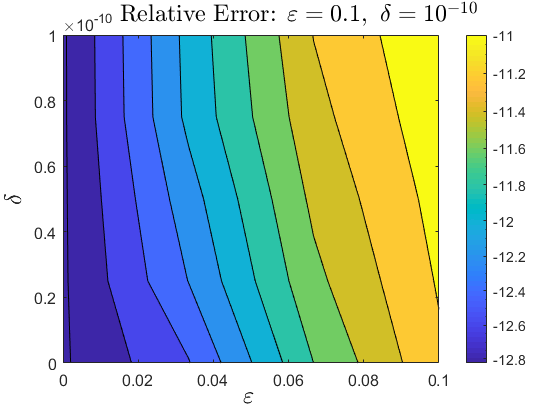
\includegraphics[width=7.6cm]{sections/7_conclusions_and_future_directions/Large_Eps_Small_Delta_2.png} }}%
    %\qquad
    \subfloat[\centering Small $\varepsilon$, Large $\delta$ ]{{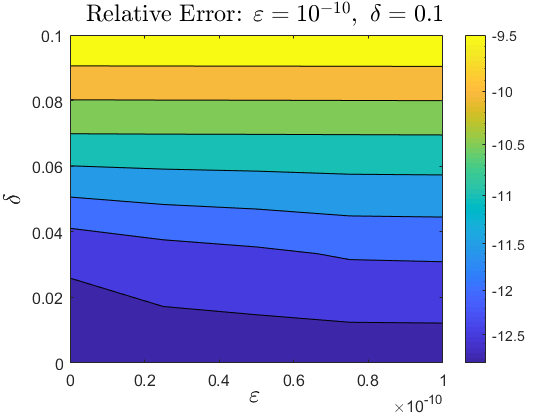
\includegraphics[width=7.6cm]{sections/7_conclusions_and_future_directions/Small_Eps_Large_Delta_2.png} }}%
    \vspace{3 mm}
    \caption{A contour plot of the relative error computed with our HOPS/AWE algorithm by holding $N=M=8$ Taylor orders fixed. In Figure $34\text{(a)}$ we expand up to $\Eps = 0.1$ and $\delta = 10^{-10}$ simultaneously with $N=M=8$ Taylor orders. In Figure $34\text{(b)}$ we expand up to $\Eps = 10^{-10}$ and $\delta = 0.1$ simultaneously with $N=M=8$ Taylor orders.}%
    \label{fig:example}%
\end{figure}
\vspace{-18mm}
Supplementary testing in both the upper and lower layers confirms that our HOPS/AWE algorithm is better suited towards larger $\varepsilon$.
%\begin{flushleft}
\newline
\\
\textbf{Predictions:} Our HOPS/AWE methodology takes advantage of exact enforcement of the \gls{owc} at an artificial boundary in order to truncate the computational domain to one of finite extent. After flattening the surface, the DNOs recover information through the solution stored at the interface. We suspect that this process mitigates large perturbations of the height/slope. By following techniques developed in \cite{NichollsReitich00b,NichollsTaber06,Nicholls16b,NichollsShen08}, we intend to rigorously prove that the TFE method is analytic when $\varepsilon$ is large. Additionally, we are interested in perturbing other physical parameters in the context of layered media problems. These are discussed in the engineering literature \cite{mashayekh2018parameter,mashayekh2018parameter2}.
\section{Rayleigh Singularities}
\label{Sec: Rayleigh Singularities}
A fundamental equation in the HOPS/AWE algorithm is
$$\alpha_p^2 + (\gamma_p^q(\delta))^2 = (k^q)^2,$$
where $k^q$ represents the wavenumber, $q\in\{u,w\}$, and $\alpha=k^q\sin(\theta), \gamma=k^q\cos(\theta),$ are parameters corresponding to refraction/reflection of the incidence angle $\theta$. As shown in $\S 5.4$, a Rayleigh singularity (or Wood's anomaly) occurs when $\ualpha_p^2 = (\uk^q)^2$ for any integer $p\neq 0$. That is, if $\ugamma_p^q(\delta) =0$ for $p\neq 0$ then the Taylor series expansion of $\gamma_p^q(\delta)$ is invalid. In \cite{Nicholls16}, the author investigated changing the Taylor expansion to a Puiseux expansion \cite{basu2007algorithms}:
$$\gamma_p^q(\delta)=\sum_{m=0}^{\infty}\gamma_{p,m}^q\delta^{m+1/2}=\delta^{1/2}\sum_{m=0}^{\infty}\gamma_{p,m}^q\delta^m.$$
However, he found that this approach ran into external difficulties ($\S$6 of \cite{Nicholls16}) simplifying explicit forms of the Dirichlet and Neumann trace operators.
\newline
\\
\textbf{Predictions:} Rayleigh singularities are a central obstruction to the convergence of our HOPS/AWE algorithm. In all of our numerical tests, we select custom frequency ranges which maximize the radius of convergence of our algorithm by expanding away from the singularities (cf. $\S 5.6$). Alternative methods such as Padé summation also fail to be analytic in a neighborhood of a Rayleigh singularity. General perturbation theory provides a variety of known techniques \cite{suslov2005divergent,convfromdiv,Heinz2020,dienes1957taylor,arteca1984summation} for expanding around divergent perturbation series. We suspect that adding these techniques to our HOPS/AWE algorithm will allow us perform a series expansion of $\ugamma_p^q(\delta)$ that does not diverge when $\ugamma_p^q(\delta)=0.$
\section{Multiple Layers}
\label{Sec: Multiple Layers}

In \cite{Nicholls16b}, the author discusses how to apply our HOPS methodology in multilayered configurations. He considers a multilayered material with $M$ (finite) interfaces at 
$$z=a^{(m)}+g^{(m)}(x,y),\quad 1\leq m \leq M,$$
which are $d_x \times d_y$ periodic
$$g^{(m)}(x+d_x,y+d_y)=g^{(m)}(x,y),\quad 1\leq m \leq M,$$
separating $(M+1)$--many layers.
%\vspace{-12mm}
\begin{figure}[H]
    \centering
    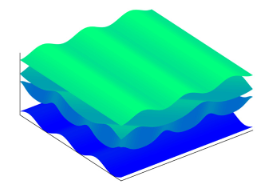
\includegraphics[width=7.6cm]{sections/7_conclusions_and_future_directions/multilayered.png}%
    \vspace{3mm}
    \caption{A five--layer problem configuration with layer interfaces $z = a^{(m)}+g^{(m)}(x).$}%
    \label{fig:example}%
\end{figure}
\vspace{-15mm}
%\begin{flushleft}
A generalization of our analyticity theorems (cf. $\S 4.5$) up to $M$ parameters is included as Theorem~$3.2$ in \cite{Nicholls16b}. For this, we consider quite general systems of linear equations of the form
%\end{flushleft}
\be
\bA(\tEps)\bV(\tEps)=\bR(\tEps),
\ee
where 
\bes
\bA(\tEps)=\sum_{\tn=0}^{\infty}\bA_{\tn}\tEps^{\tn},\quad 
\bR(\tEps) = \sum_{\tn=0}^{\infty}\bR_{\tn}\tEps^{\tn}.
\ees
The tildes represent multi--index notation \cite{Evans10}, in particular
\bes
\tEps := \begin{pmatrix} \Eps_1 \\ \vdots \\ \Eps_M \end{pmatrix},
\quad
\tn := \begin{pmatrix} n_1 \\ \vdots \\ n_M \end{pmatrix},
\ees
and the convention
\bes
\sum_{\tn=0}^{\infty} 
    A_{\tn}\ \tEps^{\tn}
  = \sum_{n_1=0}^{\infty} \cdots \sum_{n_M=0}^{\infty}
    A_{n_1,\ldots,n_M} \Eps_1^{n_1} \cdots \Eps_M^{n_M}.
\ees
As in $\S 4.5$, we seek a solution of the form
\be
\bV(\tEps)=\sum_{\tn=0}^{\infty}\bV_{\tn}\tEps^{\tn},
\ee
and from $(7.1)$ we find at order $\mathcal{O}(\tEps^{\tn})$
\bes
\bA_0\bV_{\tn}= \bR_{\tn} - \left(\sum_{\tl=0}^{\tn}\bA_{\tn-\tl}\bV_{\tl}- \bA_0\bV_{\tn}\right),
\ees
or
\be
\bV_{\tn}= \bA_0^{-1}\left\{\bR_{\tn} - \left(\sum_{\tl=0}^{\tn}\bA_{\tn-\tl}\bV_{\tl}- \bA_0\bV_{\tn}\right)\right\}.
\ee
The above notation represents multi--indices in the form
\bes
\sum_{\tl=0}^{\tn}\bA_{\tn-\tl}\bV_{\tl} = \sum_{\ell_1=0}^{n_1}\cdots \sum_{\ell_M=0}^{n_M}
    \bA_{n_1-\ell_1,\ldots,n_M-\ell_M} \bV_{\ell_1,\ldots,\ell_m},  
\ees
where $\tn=(n_1,\ldots,n_M),$ $\tl=(\ell_1,\ldots,\ell_M),$ and $0=(0,\ldots,0)$ with the convention
\bes
\tn \geq 0 \iff n_1\geq 0,\ldots,n_M\geq 0, \quad\tl \geq 0 \iff \ell_1\geq 0,\ldots,\ell_M\geq 0.
\ees
With these, we can extend our existence theorem (Theorem $4.5.1$) to $M$ parameters.
\begin{theorem}
\label{Thm:AVR}
Given two Banach spaces, $X$ and $Y$, suppose that:
\begin{enumerate}[label={\upshape[\arabic*]}]
\item $\bR_{\tn} \in Y$ for all $\tn \geq 0$,
  and there exist $M$--multi--indexed constants $C_R > 0$, $B_R > 0$,
  \bes
  C_R = \begin{pmatrix} C_{R,1} \\ \vdots \\ C_{R,M} \end{pmatrix},
  \quad
  B_R^{\tn} = \begin{pmatrix} B_{R,1}^{n_1} \\ \vdots \\ 
  B_{R,M}^{n_M} \end{pmatrix},
  \ees
  such that
  \bes
  \Norm{\bR_{\tn}}{Y} \leq C_R B_R^{\tn},
  \ees
\item $\bA_{\tn}: X \rightarrow Y$ for all
  $\tn \geq 0$, and there exist $M$--multi--indexed
  constants $C_A > 0$, $B_A > 0$ such that
  \bes
  \Norm{\bA_{\tn}}{X \rightarrow Y} \leq C_A B_A^{\tn},
  \ees
\item $\bA_0^{-1}: Y \rightarrow X$, and there 
  exists a constant $C_e > 0$ such that
  \bes
  \Norm{\bA_0^{-1}}{Y \rightarrow X} \leq C_e.
  \ees  
\end{enumerate}
Then the equation $(7.1)$ has a unique solution,
\be
\label{Eqn:V:Exp:Multi}
\bV(\tEps) = \sum_{\tn=0}^{\infty} \bV_{\tn} \tEps^{\tn},
\ee
and there exist $M$--multi--indexed constants $C_V > 0$ and $B_V > 0$ such that
\bes
\Norm{\bV_{\tn}}{X} \leq C_V B_V^{\tn},
\ees
for all $\tn \geq 0$ and any
\bes
C_V \geq 2 C_e C_R,
\quad
B_V \geq \max \left\{ B_R, 2 B_A, 2^{M+1} C_e C_A B_A \right\},
\ees
enforced componentwise. This implies that, for any $M$--multi--indexed constant
$0 \leq \tilde{\rho} < 1$, 
$(7.4)$, converges for all $\tEps$ such that
$B \tEps < \tilde{\rho}$, i.e., $\tEps < \tilde{\rho}/B$.
\end{theorem}
\begin{remark}
Our proof strategy is a form of multidimensional induction where given a statement $\bP(n_1, n_2, n_3, ..., n_M)$ for some $M\in \mathbb{N}$, we will show that $\forall n_1, n_2,\ldots, n_M \geq 0$, $\bP(n_1, n_2, n_3, ..., n_M)$ is true by inducting on $n_M$. We will follow the steps outlined below.
\begin{enumerate}
\item Establish $\bP(0,\ldots,n_j,\ldots,0)$ for all $1 \leq j < M$ and $n_1,\ldots,n_j \geq 0.$
\item Given $\bP(n_1,n_2,\ldots,n_j,\ldots,0)$ for all $1 \leq j < M$ and $n_1,\ldots,n_j \geq 0$, establish $\bP(n_1,n_2,\ldots,\bar{n}_j,\ldots,0)$. This can be accomplished through the two steps below.
\begin{enumerate}
    \item Establish $\bP(0,\ldots,\bar{n}_j,\ldots,0)$ for all $\bar{n}_j \geq 0$ (where the hypothesis in $[2]$ gives the required case for $n_j < \bar{n}_j$).
    \item Given  $\bP(n_1,n_2,\ldots,\bar{n}_j,\ldots,0)$ for all $1 \leq j < M$ and $n_1 < \bar{n}_1,  n_2 < \bar{n}_2,\ldots, $ $n_{j-1}  < \bar{n}_{j-1}$ and $\bar{n}_j\geq 0$, establish $\bP(\bar{n}_1,\bar{n}_2,\ldots,\bar{n}_j,\ldots,0)$.
\end{enumerate}
\item Given $\bP(n_1,n_2,\ldots,n_j,n_{j+1},\ldots,0)$ for all $1 \leq j+1 < M$ and $n_1,\ldots,n_{j+1} \geq 0$, establish $\bP(n_1,n_2,\ldots,n_j,\bar{n}_{j+1},\ldots,0)$. This can be accomplished by following the two steps outlined below. 
\begin{enumerate}
    \item Establish $\bP(0,\ldots,\bar{n}_{j+1},\ldots,0)$ for all $\bar{n}_{j+1} \geq 0$ (where the hypothesis in $[3]$ gives the required case for $n_{j+1} < \bar{n}_{j+1}$).
    \item Given  $\bP(n_1,n_2,\ldots,n_j,\bar{n}_{j+1},\ldots,0)$ for all $1 \leq j+1 < M$ and  $n_1 < \bar{n}_1,  n_2 < \bar{n}_2,\ldots, n_{j} < \bar{n}_{j}$ and $\bar{n}_{j+1}\geq 0$, establish $\bP(\bar{n}_1,\bar{n}_2,\ldots,\bar{n}_j,\bar{n}_{j+1}\ldots,0)$.
\end{enumerate}
\item Given $\bP(n_1,n_2,\ldots,n_{M-1},n_M)$ for all $n_1,n_2,\ldots,n_{M-1} \geq 0$ and $n_M < \bar{n}_M$, establish $\bP(n_1,n_2,\ldots,n_{M-1},\bar{n}_M)$. This can be accomplished by the two steps below (the base cases are handled through $[2]$ and $[3]$).
\begin{enumerate}
    \item Establish $\bP(0,\ldots,\bar{n}_{M})$ for $\bar{n}_{M} \geq 0$ (where the hypothesis in $[4]$ handles the required case for  $n_{M} < \bar{n}_{M}$).
    \item Given $\bP(n_1,n_2,\ldots,n_{M-1},\bar{n}_M)$ for all $n_1 < \bar{n}_1, n_2 < \bar{n}_2, \ldots n_{M-1} < \bar{n}_{M-1}$ and $\bar{n}_M \geq 0$, establish $\bP(\bar{n}_1,\bar{n}_2,\ldots,\bar{n}_{M-1},\bar{n}_M)$.
\end{enumerate}
\end{enumerate}

\end{remark}

\begin{proof}{[Theorem 7.4.1]} As with $\tEps$ and $\tn$, we represent $\tilde{\rho}$ by
\bes
\tilde{\rho} := \begin{pmatrix} \rho_1 \\ \vdots \\ \rho_M \end{pmatrix}.
\ees
As before, we will work by induction and consider the general case for finite $M>0$ where we want to establish
\bes
\norm{\bV_{n_1,\ldots,n_M}}_X \leq C_{V,1}\ldots C_{V,M} B_{V,1}^{n_1}\ldots B_{V,M}^{n_M}, \quad \forall n_1,\ldots,n_M\geq 0.
\ees
We prove this via an induction on $n_M$. The base case $n_1,n_2,\ldots, n_{j-1},n_{j+1},\ldots,$ $n_M=0$ and $1 \leq j < M$:
\bes
\norm{\bV_{0,\ldots,n_j,\ldots,0}}_X \leq C_{V,j} B_{V,j}^{n_j}, \quad \forall n_j\geq 0,
\ees
has previously been established by Theorem $4.5.1$ where $\tEps = \Eps_j$ and $\delta=0$. We now assume
\bes
\norm{\bV_{n_1,\ldots,n_j,\ldots,0}}_X \leq  C_{V,1}\ldots C_{V,j}B_{V,1}^{n_1}\ldots B_{V,j}^{n_j}, ~~ \forall n_1,\ldots,n_{j-1}\geq 0,~~ \forall n_j < \bar{n}_j,~~ 1 \leq j < M,
\ees
and seek
\bes
\norm{\bV_{n_1,\ldots,\bar{n}_j,\ldots,0}}_X \leq  C_{V,1}\ldots C_{V,j}B_{V,1}^{n_1}\ldots B_{V,j}^{\bar{n}_j}, ~~ \forall n_1,\ldots,n_{j-1}\geq 0.
\ees
This can be obtained through a chain of $(M-1)$ inductions on $n_1,\ldots,n_j$ where $1 \leq j < M$. For simplicity, we will show what happens in the arbitrary case $n_j$. The base case $n_1,\ldots,n_{j-1}=0$:
\bes
\norm{\bV_{0,\ldots,\bar{n}_j,\ldots,0}}_X \leq  C_{V,j}B_{V,j}^{\bar{n}_j}, \quad \forall \bar{n}_j \geq 0,
\ees
is established by Theorem $4.5.1$ where $\tEps = \Eps_j$ and $\delta=0$. Therefore, we assume
\begin{align*}
\norm{\bV_{n_1,\ldots,\bar{n}_j,\ldots,0}}_X \leq  C_{V,1}\ldots C_{V,j}B_{V,1}^{n_1}\ldots B_{V,j}^{\bar{n}_j},~~\forall n_1  &< \bar{n}_1,\ldots, n_{j-1} < \bar{n}_{j-1},~~ \forall \bar{n}_j \geq 0,\\&~ 1 \leq j < M,
\end{align*}
and seek
\bes
\norm{\bV_{\bar{n}_1,\ldots,\bar{n}_j,\ldots,0}}_X \leq  C_{V,1}\ldots C_{V,j}B_{V,1}^{\bar{n}_1}\ldots B_{V,j}^{\bar{n}_j}.
\ees
Recalling $\tn=(n_1,\ldots,n_j)$ and  $\tl=(\ell_1,\ldots,\ell_j)$, we define
\be
{\sum_{\tl=0}^{\tn}}^{*}\bA_{\tn-\tl}\bV_{\tl} := \sum_{\tl=0}^{\tn}\bA_{\tn-\tl}\bV_{\tl} - \bA_0\bV_{\tn},
\ee
and apply $(7.3),(7.5)$ and the mapping properties of $\bA_{0}^{-1}$ to find
\bes
\norm{\bV_{\bar{n}_1,\ldots,\bar{n}_j,\ldots,0}}_X\leq C_e\left\{\norm{\bR_{\bar{n}_1,\ldots,\bar{n}_j}}_Y + {\sum_{\tl=0}^{\tn}}^{*}\norm{\bA_{\tn-\tl}\bV_{\tl}}_Y\right\}.
\ees
Using the estimates on $\bR_{n_1,\ldots,n_j}$ and $\bA_{n_1,\ldots,n_j}$ (for all $n_1,\ldots,n_j$) and $\bV_{n_1,\ldots,n_j}$ $(n_1 < \bar{n}_1, \ldots, n_j < \bar{n}_j)$ we have
\begin{align*}
\norm{\bV_{\bar{n}_1,\ldots,\bar{n}_j,\ldots,0}}_X &\leq
C_e\Bigg\{C_{R,1}\ldots C_{R,j}B_{R,1}^{\bar{n}_1}\ldots B_{R,j}^{\bar{n}_j} + {\sum_{\tl=0}^{\tn}}^{*}C_{A,1}\ldots C_{A,j}B_{A,1}^{\bar{n}_1-\ell_1}\ldots B_{A,j}^{\bar{n}_j-\ell_j}\\ & \qquad \qquad \qquad \qquad \qquad \qquad \qquad \qquad \times
C_{V,1}\ldots C_{V,j}B_{V,1}^{\ell_1}\ldots B_{V,j}^{\ell_j}\Bigg\} \\& =
C_eC_{R,1}\ldots C_{R,j}B_{R,1}^{\bar{n}_1}\ldots B_{R,j}^{\bar{n}_j} + C_eC_{A,1}\ldots C_{A,j}C_{V,1}\ldots C_{V,j} \\&
~~ \times \left(\frac{B_{A,1}}{B_{V,1}}\right)B_{V,1}^{\bar{n}_1}\cdots \left(\frac{B_{A,j}}{B_{V,j}}\right)B_{V,j}^{\bar{n}_j}{\sum_{\tl=0}^{\tn}}^{*}
\left(\frac{B_{A,1}}{B_{V,1}}\right)B_{V,1}^{\bar{n}_1-\ell_1-1}\cdots \\& ~~ \times
\left(\frac{B_{A,j}}{B_{V,j}}\right)B_{V,j}^{\bar{n}_j-\ell_j-1} \\& \leq
C_eC_{R,1}\ldots C_{R,j}B_{V,1}^{\bar{n}_1}\ldots B_{V,j}^{\bar{n}_j} + C_eC_{A,1}\ldots C_{A,j}C_{V,1}\ldots C_{V,j} \\& ~~ \times
\left(\frac{B_{A,1}}{B_{V,1}}\right)B_{V,1}^{\bar{n}_1}\cdots\left(\frac{B_{A,j}}{B_{V,j}}\right)B_{V,j}^{\bar{n}_j}\left(\frac{1}{1-1/2}\right)^j,
\end{align*}
if $B_{A,k}/B_{V,k} \leq 1/2$, $k=1,\ldots,j$ (implying $B_{V,k} \geq 2B_{A,k}$). We are done if we demand that
\bes
B_{V,k} \geq B_{R,k}, \quad C_eC_{R,k} \leq C_{V,k}/2, \quad 2^jC_eC_{A,k}C_{V,k}(B_{A,k}/B_{V,k}) \leq 
C_{V,k}/2.
\ees
This can be realized if
\bes
C_{V,k} \geq 2C_eC_{R,k}, \quad
B_{V,k} \geq \max\left\{B_{R,k},2B_{A,k},2^{j+1}C_eC_{A,k}B_{A,k}\right\}.
\ees
We then assume
\begin{align*}
\norm{\bV_{n_1,\ldots,n_{j+1},\ldots,0}}_X \leq  C_{V,1}\ldots C_{V,j+1}B_{V,1}^{n_1}\ldots B_{V,j+1}^{n_{j+1}}, ~~ &\forall n_1,\ldots,n_j\geq 0,~~ \forall n_{j+1} < \bar{n}_{j+1},\\&~~ 1 \leq j < M,
\end{align*}
and seek
\bes
\norm{\bV_{n_1,\ldots,\bar{n}_{j+1},\ldots,0}}_X \leq  C_{V,1}\ldots C_{V,j+1}B_{V,1}^{n_1}\ldots B_{V,j+1}^{\bar{n}_{j+1}}, ~~ \forall n_1,\ldots,n_{j}\geq 0.
\ees
As before, this can be obtained through a chain of $M$ inductions on $n_1,\ldots,n_{j+1}$ where $1 \leq j < M$. For simplicity, we will show what happens in the arbitrary case $n_{j+1}$. The base case $n_1,\ldots,n_{j}=0$:
\bes
\norm{\bV_{0,\ldots,\bar{n}_{j+1},\ldots,0}}_X \leq  C_{V,j+1}B_{V,j+1}^{\bar{n}_{j+1}}, \quad \forall \bar{n}_{j+1} \geq 0,
\ees
is established by Theorem $4.5.1$ where $\tEps = \Eps_{j+1}$ and $\delta=0$. Therefore, we assume
\begin{align*}
\norm{\bV_{n_1,\ldots,\bar{n}_{j+1},\ldots,0}}_X \leq  C_{V,1}\ldots C_{V,j+1}B_{V,1}^{n_1}\ldots B_{V,j+1}^{\bar{n}_{j+1}},~~\forall n_1  &< \bar{n}_1,\ldots, n_{j} < \bar{n}_{j},~~ \forall \bar{n}_{j+1} \geq 0,\\&~ 1 \leq j < M,
\end{align*}
and seek
\bes
\norm{\bV_{\bar{n}_1,\ldots,\bar{n}_{j+1},\ldots,0}}_X \leq  C_{V,1}\ldots C_{V,j+1}B_{V,1}^{\bar{n}_1}\ldots B_{V,j+1}^{\bar{n}_{j+1}}.
\ees
In this scenario, $\tn=(n_1,\ldots,n_{j+1})$ and  $\tl=(\ell_1,\ldots,\ell_{j+1}),$ so we apply $(7.3),(7.5)$ and the mapping properties of $\bA_{0}^{-1}$ to find
\bes
\norm{\bV_{\bar{n}_1,\ldots,\bar{n}_{j+1},\ldots,0}}_X\leq C_e\left\{\norm{\bR_{\bar{n}_1,\ldots,\bar{n}_{j+1}}}_Y + {\sum_{\tl=0}^{\tn}}^{*}\norm{\bA_{\tn-\tl}\bV_{\tl}}_Y\right\}.
\ees
Using the estimates on $\bR_{n_1,\ldots,n_{j+1}}$ and $\bA_{n_1,\ldots,n_{j+1}}$ (for all $n_1,\ldots,n_{j+1}$) and $\bV_{n_1,\ldots,n_{j+1}}$ $(n_1 < \bar{n}_1, \ldots, n_{j+1} < \bar{n}_{j+1})$ we have
\begin{align*}
\norm{\bV_{\bar{n}_1,\ldots,\bar{n}_{j+1},\ldots,0}}_X &\leq
C_e\Bigg\{C_{R,1}\ldots C_{R,{j+1}}B_{R,1}^{\bar{n}_1}\ldots B_{R,{j+1}}^{\bar{n}_{j+1}} + {\sum_{\tl=0}^{\tn}}^{*}C_{A,1}\ldots C_{A,{j+1}}B_{A,1}^{\bar{n}_1-\ell_1}\ldots \\ & \qquad \qquad \qquad \qquad \qquad \quad \times
B_{A,{j+1}}^{\bar{n}_{j+1}-\ell_{j+1}}C_{V,1}\ldots C_{V,{j+1}}B_{V,1}^{\ell_1}\ldots B_{V,{j+1}}^{\ell_{j+1}}\Bigg\} \\& =
C_eC_{R,1}\ldots C_{R,{j+1}}B_{R,1}^{\bar{n}_1}\ldots B_{R,{j+1}}^{\bar{n}_{j+1}} + C_eC_{A,1}\ldots C_{A,{j+1}}C_{V,1}\ldots C_{V,{j+1}} \\&
~~ \times \left(\frac{B_{A,1}}{B_{V,1}}\right)B_{V,1}^{\bar{n}_1}\cdots \left(\frac{B_{A,{j+1}}}{B_{V,{j+1}}}\right)B_{V,{j+1}}^{\bar{n}_{j+1}}{\sum_{\tl=0}^{\tn}}^{*}
\left(\frac{B_{A,1}}{B_{V,1}}\right)B_{V,1}^{\bar{n}_1-\ell_1-1}\cdots \\& ~~ \times
\left(\frac{B_{A,{j+1}}}{B_{V,{j+1}}}\right)B_{V,{j+1}}^{\bar{n}_{j+1}-\ell_{j+1}-1} \allowdisplaybreaks\\& \leq
C_eC_{R,1}\ldots C_{R,{j+1}}B_{V,1}^{\bar{n}_1}\ldots B_{V,{j+1}}^{\bar{n}_{j+1}} + C_eC_{A,1}\ldots C_{A,{j+1}}C_{V,1}\ldots C_{V,{j+1}} \\& ~~ \times
\left(\frac{B_{A,1}}{B_{V,1}}\right)B_{V,1}^{\bar{n}_1}\cdots\left(\frac{B_{A,{j+1}}}{B_{V,{j+1}}}\right)B_{V,{j+1}}^{\bar{n}_{j+1}}\left(\frac{1}{1-1/2}\right)^{j+1},
\end{align*}
if $B_{A,t}/B_{V,t} \leq 1/2$, $t=1,\ldots,j+1$ (implying $B_{V,t} \geq 2B_{A,t}$). We are done if we demand that
\bes
B_{V,t} \geq B_{R,t}, \quad C_eC_{R,t} \leq C_{V,t}/2, \quad 2^{j+1}C_eC_{A,t}C_{V,t}(B_{A,t}/B_{V,t}) \leq 
C_{V,t}/2.
\ees
This can be realized if
\bes
C_{V,t} \geq 2C_eC_{R,t}, \quad
B_{V,t} \geq \max\left\{B_{R,t},2B_{A,t},2^{j+2}C_eC_{A,t}B_{A,t}\right\}.
\ees
To complete the general case for finite $M>0$, we assume
\bes
\norm{\bV_{n_1,\ldots,n_M}}_X \leq  C_{V,1}\ldots C_{V,M}B_{V,1}^{n_1}\ldots B_{V,M}^{n_M}, ~~ \forall n_1,\ldots,n_{M-1}\geq 0,~~ \forall n_M < \bar{n}_M,
\ees
and seek
\bes
\norm{\bV_{n_1,\ldots,\bar{n}_M}}_X \leq  C_{V,1}\ldots C_{V,M}B_{V,1}^{n_1}\ldots B_{V,M}^{\bar{n}_M}, ~~ \forall n_1,\ldots,n_{M-1}\geq 0.
\ees
The base case $n_1,n_2,\ldots,n_{M-1}=0$:
\bes
\norm{\bV_{0,\ldots,\bar{n}_M}}_X \leq  C_{V,M}B_{V,M}^{\bar{n}_M}, \quad \forall \bar{n}_M \geq 0,
\ees
has previously been established by Theorem $4.5.1$ where $\tEps = \Eps_M$ and $\delta =0$. Finally, we assume
\begin{align*}
\norm{\bV_{n_1,\ldots,n_{M-1},\bar{n}_M}}_X \leq  C_{V,1}\ldots C_{V,M}B_{V,1}^{n_1}\ldots B_{V,M}^{\bar{n}_M},~~~&\forall n_1  < \bar{n}_1,\ldots, n_{M-1} < \bar{n}_{M-1},\\&~~~~ \forall \bar{n}_M \geq 0,
\end{align*}
and seek
\bes
\norm{\bV_{\bar{n}_1,\ldots,\bar{n}_{M-1},\bar{n}_M}}_X \leq  C_{V,1}\ldots C_{V,M}B_{V,1}^{\bar{n}_1}\ldots B_{V,M}^{\bar{n}_M}.
\ees
In this case, $\tn=(n_1,\ldots,n_M)$ and  $\tl=(\ell_1,\ldots,\ell_M),$ so we apply $(7.3),(7.5)$ and the mapping properties of $\bA_{0}^{-1}$ to find
\bes
\norm{\bV_{\bar{n}_1,\ldots,\bar{n}_M}}_X\leq C_e\left\{\norm{\bR_{\bar{n}_1,\ldots,\bar{n}_M}}_Y + {\sum_{\tl=0}^{\tn}}^{*}\norm{\bA_{\tn-\tl}\bV_{\tl}}_Y\right\}.
\ees
Using the estimates on $\bR_{n_1,\ldots,n_M}$ and $\bA_{n_1,\ldots,n_M}$ (for all $n_1,\ldots,n_M$) and $\bV_{n_1,\ldots,n_M}$ $(n_1 < \bar{n}_1, \ldots, n_M < \bar{n}_M)$ we have
\vspace{-1.5mm}
\begin{align*}
\norm{\bV_{\bar{n}_1,\ldots,\bar{n}_M}}_X &\leq
C_e\Bigg\{C_{R,1}\ldots C_{R,M}B_{R,1}^{\bar{n}_1}\ldots B_{R,M}^{\bar{n}_M} + {\sum_{\tl=0}^{\tn}}^{*}C_{A,1}\ldots C_{A,M}B_{A,1}^{\bar{n}_1-\ell_1}\ldots B_{A,M}^{\bar{n}_M-\ell_M}\\ & \qquad \qquad \qquad \qquad \qquad \qquad \qquad \qquad \times
C_{V,1}\ldots C_{V,M}B_{V,1}^{\ell_1}\ldots B_{V,M}^{\ell_M}\Bigg\} \\& =
C_eC_{R,1}\ldots C_{R,M}B_{R,1}^{\bar{n}_1}\ldots B_{R,M}^{\bar{n}_M} + C_eC_{A,1}\ldots C_{A,M}C_{V,1}\ldots C_{V,M} \\& 
~~ \times \left(\frac{B_{A,1}}{B_{V,1}}\right)B_{V,1}^{\bar{n}_1}\cdots \left(\frac{B_{A,M}}{B_{V,M}}\right)B_{V,M}^{\bar{n}_M}{\sum_{\tl=0}^{\tn}}^{*}
\left(\frac{B_{A,1}}{B_{V,1}}\right)B_{V,1}^{\bar{n}_1-\ell_1-1}\cdots \\& \allowdisplaybreaks~~ \times
\left(\frac{B_{A,M}}{B_{V,M}}\right)B_{V,M}^{\bar{n}_M-\ell_M-1} \\&  \leq
C_eC_{R,1}\ldots C_{R,M}B_{V,1}^{\bar{n}_1}\ldots B_{V,M}^{\bar{n}_M} + C_eC_{A,1}\ldots C_{A,M}C_{V,1}\ldots C_{V,M} \\& ~~ \times
\left(\frac{B_{A,1}}{B_{V,1}}\right)B_{V,1}^{\bar{n}_1}\cdots\left(\frac{B_{A,M}}{B_{V,M}}\right)B_{V,M}^{\bar{n}_M}\left(\frac{1}{1-1/2}\right)^M,
\end{align*}
if $B_{A,i}/B_{V,i} \leq 1/2$, $i=1,\ldots,M$ (implying $B_{V,i} \geq 2B_{A,i}$). We are done if we demand that
\bes
B_{V,i} \geq B_{R,i}, \quad C_eC_{R,i} \leq C_{V,i}/2, \quad 2^MC_eC_{A,i}C_{V,i}(B_{A,i}/B_{V,i}) \leq 
C_{V,i}/2.
\ees
This can be realized if
\bes
C_{V,i} \geq 2C_eC_{R,i}, \quad
B_{V,i} \geq \max\left\{B_{R,i},2B_{A,i},2^{M+1}C_eC_{A,i}B_{A,i}\right\}.
\ees
\end{proof}
Using a similar approach in conjunction with the analysis in Chapters $2$ and $3$, we predict a more general form of Theorems $2.9.2$ and $3.8.1$ exists, which would establish the analyticity of the transformed field with respect to any finite $M > 0$ perturbation parameters.
\vspace{1mm}
\begin{conjecture} 
\label{Conj:u,w:Anal:n:n_m}
Given any integer $s \geq 0$, if $f \in C^{s+2}([0,d])$ and 
$U_{\tilde{n}} \in H^{s+3/2}([0,d])$, $W_{\tilde{n}}\in H^{s+3/2}([0,d])$ such that
\bes
\|U_{\tilde{n}}\|_{H^{s+3/2}} \le K_U B_U^{\tn} , \quad
\|W_{\tilde{n}}\|_{H^{s+3/2}} \le K_W B_W^{\tn} ,
\ees
for constants $K_U, K_W>0$ and $M$--multi--indexed constants $B_U, B_W > 0$, then 
$u_{\tn} \in H^{s+2}([0,d]\times[0,a])$, $w_{\tn}\in H^{s+2}([0,d]\times[-b,0])$ and
\bes
\label{Eqn:u,w:Est:n:n_m}
\|u_{\tn}\|_{H^{s+2}} \le K B^{\tn}, \quad
\|w_{\tn}\|_{H^{s+2}} \le \tilde{K}\tilde{B}^{\tn} ,
\ees
for constants $K,\tilde{K}> 0$ and $M$--multi--indexed constants $B ,\tilde{B}>0$.
\end{conjecture}
\vspace{1mm}
Analogously, a similar procedure would establish a more general form of Theorems $2.10.2$ and $3.9.2$ for the analyticity of the DNOs for any finite $M>0$ perturbation parameters.
\vspace{1mm}
\begin{conjecture} 
\label{Thm:G,J:Anal:n:n_m}
Given any integer $s \geq 0$, if $f \in C^{s+2}([0,d])$ and 
$U_{\tn} \in H^{s+3/2}([0,d])$, $W_{\tn} \in H^{s+3/2}([0,d])$ such that
\bes
\SobNorm{U_{\tn}}{s+3/2} \leq K_U B_U^{\tn}, \quad
\SobNorm{W_{\tn}}{s+3/2} \leq K_W B_W^{\tn},
\ees
for constants $K_U,K_W> 0$ and $M$--multi--indexed constants $B_U, B_W > 0$, then $G_{\tn} \in H^{s+1/2}([0,d])$, $J_{\tn} \in H^{s+1/2}([0,d])$ and
\bes
\label{Eqn:G,J:Est:n:n_m} 
\|G_{\tn}\|_{H^{s+1/2}} \le \tilde{K}\tilde{B}^{\tn}, \quad
\|J_{\tn}\|_{H^{s+1/2}} \le \dbtilde{K} \dbtilde{B}^{\tn},
\ees
for constants $\tilde{K},\dbtilde{K}  > 0$ and $M$--multi--indexed constants $\tilde{B},\dbtilde{B}>0$.
\end{conjecture}
\vspace{1mm}
Upon proving these, one has two key ingredients to the more general version of Theorem $4.6.1$ which establishes the existence and uniqueness of solutions to a system of partial differential equations with respect to $M$ perturbation parameters.
\vspace{1mm}
\begin{conjecture} 
\label{Conj:Main}
Given an integer $s \geq 0$, if $f \in C^{s+2}([0,d])$ then the 
equation $(7.1)$ has a unique solution, $(7.4)$,
and there exist a constant $C > 0$ and $M$--multi--indexed constants $B>0$ such that
\bes
\Norm{\bV_{\tn}}{X^s} \leq C B^{\tn},
\ees
for all $\tn \geq 0$.  This implies that for any $M$--multi--indexed constant
$0 \leq \tilde{\rho} < 1$, $(7.4)$, converges for all $\tEps$ such that
$B \tEps < \tilde{\rho}$, i.e., $\tEps < \tilde{\rho}/B$.
\end{conjecture}
\vspace{1mm}
\textbf{Predictions:} In application oriented fields such as signal processing or sea ice modeling, practitioners work with  multiple frequencies \cite{qiu2005high,bosse1995model,zhao2009multi,blanchard2021high} at short or long wavelengths. Also, as depicted in Figure $35$, the grating surface could have $M$ different layers \cite{imperatore2017perturbation} with distinct values of $g_j(x)=\Eps f_j(x),~j=1,\ldots, M$. A proof of Conjecture $7.4.4$ would enable the freedom to enforce any number of perturbation parameters and obtain an analytic solution. Given the widespread availability of parallel computing resources coupled with additional perturbation parameters associated with elastic media, we believe that future research will force hundreds or even thousands of distinct perturbation parameters, all of which should yield an analytic solution.
\section{Parallel Programming}
\setcounter{section}{5}
\label{Sec: Parallel Programming}

In the case of multiple layered interfaces, we need to compute intermediate DNOs for up to $M$ layers. This will greatly increase the computational cost and execution time of our HOPS/AWE algorithm and we suspect that it will be necessary to introduce parallel programming techniques to offset the computational expense. In the context of the \gls{oe} method, preliminary work \cite{fang2015operator} has been completed in C\texttt{++} to parallelize the computation of Navier's equations \cite{BillinghamKing00,achenbach2012wave}. These techniques can be adapted to the TFE method through the choice of OpenMP \cite{chandra2001parallel}, MPI \cite{snir1998mpi}, or CUDA \cite{sanders2010cuda}.
\newline
\\
\textbf{Predictions:} In two or three dimensions, our HOPS code is robust, efficient and has a runtime less than an hour. A local machine with an Intel Core i$5$ CPU, $8$GB of RAM, and Windows $10$ OS completed almost every simulation in this thesis in less than thirty minutes. However, with ten to one hundred layer configurations, we suspect that many simulations will take on the order of weeks or even months. As a result, it will be necessary to parallelize our Matlab code in a compiled programming language such as C or  C\texttt{++}.

\section{Alternatives to DNOs}
\label{Sec: Alternatives to DNOs}
In Chapter $4$ we wrote our scattering problem as a linear system
\bes
\bA \bV = \bR,
\ees
where, upon expanding $\{\bA,\bV,\bR\}$ in both $\varepsilon$ and $\delta$, we arrived at the flat--interface solution $\bA_{0,0}\bV_{0,0}=\bR_{0,0}$
at order $\mathcal{O}(\varepsilon^0,\delta^0)$. We then saw it was necessary to invert
\bes
\bA_{0,0} = \begin{pmatrix}I & -I\\
-G_{0,0} & -\tau^2J_{0,0}\end{pmatrix}, 
\ees
which features the two DNOs, $G_{0,0}$ and $J_{0,0}$, in order to show the existence and uniqueness of solutions. A primary feature of all HOPS schemes is the inversion of a single, sparse operator $\bA_{0,0}$ through the use of DNOs. However, one may ponder if a different technique could produce a more competitive algorithm that is comparable to our HOPS/AWE algorithm (or even better). Is it absolutely necessary to pass in transformed field data in order to efficiently compute and recover internal information stored at the grating surface?
\\
\newline
\textbf{Predictions:} A primary advantage of our HOPS/AWE scheme is that for every perturbation order, it is only necessary to invert a single sparse operator corresponding to a flat--interface, order--zero approximation. There are a number of competing approaches in general perturbation theory within the context of layered media problems. In regards to electromagnetic wave scattering, Galerkin and boundary element methods are discussed in \cite{escapil2020helmholtz,silva2017quantifying,nakata1990boundary,elschner2012optimization,rathsfeld2006} and a high--order perturbation approach based on boundary integral equations in \cite{dolz2020higher}. High--order schemes for linear waves can be computed using level set methods \cite{sethian1999level} and fast marching methods, as well as other methods involving domain decomposition \cite{el2004comparing,benamou1997domain,larsson1999domain,gong2021convergence,perez2018domain,chan1994domain}. A holistic evaluation of these competing methods could potentially improve our HOPS/AWE algorithm if we found a faster method of inverting linear operators without the use of DNOs.
\section{Computational Complexity}
\label{Sec: Computational Complexity}

One of the fundamental reasons for developing our HOPS/AWE algorithm is its advantageous computational complexity for problems within its domain of applicability.
In comparison with other classical methods, our HOPS/AWE approach has several advantages for computing quantities such as the Reflectivity Map, $R=R(\varepsilon,\delta)$. To demonstrate this we begin
by fixing the problem of computing $R$ for $N_{\Eps}$ many values of 
$\Eps$ and $N_{\delta}$ many values of $\delta$.

In the case of computing the DNOs $G$ and $J$, we recall from $\S 2.11$ and $\S 3.10$ that our HOPS/AWE algorithm requires
$N_x \times N_z$ unknowns at every perturbation order, $(n,m)$, corresponding to
the $N_x$ equally--spaced gridpoints in the lateral direction and the $N_z + 1$ collocation points in the vertical dimension. In $\S 4.5$ we saw that we could write our scattering problem as $\bA(\Eps,\delta) \bV(\Eps,\delta) = \bR(\Eps,\delta)$ where
\bes
    \bA(\Eps,\delta)=\sumn \summ \bA_{n,m}\Eps^n\delta^m, \quad \bR(\Eps,\delta) = \sumn \summ \bR_{n,m}\Eps^{n}\delta^m,
\ees
and
\bes
\label{Eqn:Soln:Two_Param_Append}
\bV(\Eps,\delta) = \sumn \summ \bV_{n,m}\Eps^{n}\delta^m.
\ees
At order $\mathcal{O}(\Eps^n,\delta^m)$ this becomes
\begin{align}
\begin{split}
\bA_{0,0}\bV_{n,m}=&~\bR_{n,m}-\sum_{\ell=0}^{n-1}\bA_{n-\ell,0}\bV_{\ell,m}-\sum_{r=0}^{m-1}\bA_{0,m-r}\bV_{n,r}\\&
-\sum_{\ell=0}^{n-1}\sum_{r=0}^{m-1}\bA_{n-\ell,m-r}\bV_{\ell,r}.
\end{split}
\end{align}
A careful study of $(7.6)$
reveals that the computational complexity of forming the
right--hand side at order $(n,m)$ is
\bes
\BigOh{n m N_x \log(N_x) N_z \log(N_z)}.
\ees
Inverting the operator $\bA_{0,0}$ has complexity $\BigOh{N_x \log(N_x) N_z \log(N_z)}$
so the full cost of computing the $\bV_{n,m}$, 
$\{ 0 \leq n \leq N, 0 \leq m \leq M \}$, is
\bes
\BigOh{N^2 M^2 N_x \log(N_x) N_z \log(N_z)}.
\ees
Once these coefficients are recovered, the cost of summing the series in 
$(\Eps,\delta)$ is minimal, provided it is done in an efficient manner 
(e.g., by Horner's rule \cite{BurdenFaires,AtkinsonHan01}). Our algorithm then 
requires an additional $\BigOh{N_{\Eps} N_{\delta}}$ steps to sum 
over every value of $(\Eps,\delta)$, therefore the full cost of 
computing the Reflectivity Map by our HOPS/AWE method is
\be
\BigOh{N^2 M^2 N_x \log(N_x) N_z \log(N_z) + N_{\Eps} N_{\delta}}.
\ee
In contrast, for a single $(\Eps,\delta)$ pair, a Boundary Integral Method solver with $N_x$ lateral
gridpoints requires time proportional to $\BigOh{N_x^3}$ for Gaussian elimination
to solve the resulting dense system of $N_x$ equations in $N_x$ unknowns
\cite{BurdenFaires,AtkinsonHan01,ColtonKress13}. Applying this 
$N_{\Eps} \times N_{\delta}$ times results in a total computational complexity of
\be
\BigOh{N_x^3 N_{\Eps} N_{\delta}}.
\ee
Thus, once $N_{\Eps}$ and $N_{\delta}$ become large, e.g.,

\bes
N_{\Eps} N_{\delta} > \frac{N^2 M^2 N_x \log(N_x) N_z \log(N_z)}{N_x^3},
\ees
our new algorithm becomes far more efficient. We speculate that the cost of $(7.7)$ could be reduced to
\be
\BigOh{N M \log(NM)N_x \log(N_x) N_z \log(N_z) + N_{\Eps} N_{\delta}},
\ee
provided that we develop a more efficient method of computing the $\bV_{n,m}$, 
$\{ 0 \leq n \leq N, 0 \leq m \leq M \}$, such as reducing the problem space at every step. Alternative approaches to layered media problems have also been proposed by other authors \cite{bai2004reduction,chew2005fast}, including interpolation \cite{atkins2010fast} and Green's function \cite{konno2016fast}.
\newline
\\
\textbf{Predictions:} The combination of implementing parallel programming techniques (through, e.g., OpenMP or CUDA) and reducing the problem space at every step will greatly enhance the speed and fidelity of our HOPS/AWE algorithm. Considering the natural advantage surface methods have over conventional methods, such as finite difference, finite element, and spectral element methods, we expect that our HOPS/AWE algorithm will be among the most competitive available for periodic layered media problems.
\chapter{Conclusions and Future Work}
\label{sec:conclusions_and_future_dir}

\fancyhead[LO]{\text{Chapter 7}\quad \text{Conclusions and Future Work}}

This thesis establishes a novel HOPS/AWE algorithm that is particularly well suited to simulating scattering returns for periodic media problems. Our main contribution is that of Theorem $4.6.1$ which guarantees the existence and uniqueness of solutions to a system of partial differential equations which model the interaction of linear waves in periodic layered structures with respect to multiple perturbation parameters. Through the introduction of DNOs and a change of variables based on the TFE methodology, we have shown that solutions to the Helmholtz problem are jointly analytic with respect to both interfacial and frequency perturbations. As a result, our HOPS/AWE algorithm is able to handle a variety of numerical simulations that are physically challenging in both the TE and TM polarization modes. Moreover, our extensive numerical results demonstrate the accuracy, speed, and robustness expected of all HOPS methods.


\section{Future Directions}
\label{Sec: Future Directions}
There are a wide range of improvements to both the HOPS/AWE algorithm and the proof of analyticity for linear waves in periodic layered media. Our main goals for future research are to expand the TFE method through a new proof of convergence, investigate expanding around singularities, evaluate analyticity theorems in multilayered configurations, add new parallel programming functionality, explore alternative methods to recover surface data without Dirichlet--Neumann Operators, and to reduce the execution time of the HOPS algorithm. We now summarize these six research goals and suggest predictions for future research.
\begin{enumerate}[labelsep=0ex,align=left,start=1]
    \item[\textbf{Goal 1-}] ~\textbf{Choice of Parameters: Does the geometry of the perturbation impact how large the size of the perturbation can be? }
    \item[\textbf{Goal 2-}] ~\textbf{Rayleigh Singularities: Can we build a full HOPS algorithm based on points where the Taylor expansion is invalid? }
    \item[\textbf{Goal 3-}] ~\textbf{Multiple Layers: Can we prove analyticity results when the number of layers is greater than three? Do the same theorems hold for ten or one hundred layers?} 
    \item[\textbf{Goal 4-}] ~\textbf{{Parallel Programming}: Can we implement parallel programming techniques so that our HOPS code runs on $N$ processors? }
    \item[\textbf{Goal 5-}] ~\textbf{{Alternatives to DNOs}: Do we need to use DNOs to recover surface data from information stored in the transformed field? Is there an alternative method which preserves the inversion of a single, sparse operator at the interface?   }
    \item[\textbf{Goal 6-}] ~\textbf{Computational Costs: Can we reduce the execution time per time step in our HOPS algorithm?} 
\end{enumerate}

\section{Choice of Parameters}
\label{Sec: Choice of Parameters}
Our HOPS/AWE algorithm is based on two smallness assumptions:
\begin{enumerate}
\item \text{Boundary Perturbation: $g(x)=\varepsilon f(x),$ $\varepsilon\in\mathbb R$, $\varepsilon \ll 1$,}
\vspace{-2mm}
\item \text{Frequency Perturbation: $\omega=(1+\delta)\underline{\omega}=\underline{\omega}+\delta\underline{\omega},$ $\omega\in\mathbb R$, $\delta \ll 1$,} 
\end{enumerate}
with the additional assumption that $f$ is sufficiently smooth ($f\in C^2$ \cite{NichollsReitich99,NichollsReitich03b} or even Lipschitz \cite{hu2005analyticity}). Numerical simulations show that our HOPS/AWE algorithm can handle larger perturbations of $\varepsilon$ (the height/slope) in comparison to $\delta$ (the frequency). With modest test parameters and a period of $d=2\pi$, we are able to perturb the value of $\varepsilon$ (to $\varepsilon=0.1$ or even $\varepsilon=0.2$) and still get reasonable convergence results. At a value around $\varepsilon = 10^{-4}$, our HOPS/AWE algorithm converges to machine precision provided that we sum to high enough Taylor orders.
\vspace{-13mm}
\begin{figure}[H]
    \centering
    \subfloat[\centering Large $\varepsilon$, Small $\delta$ ]{{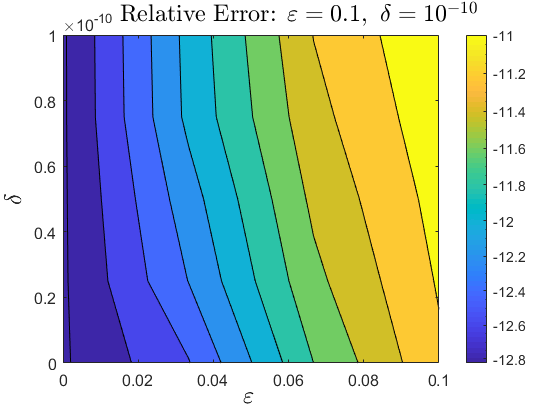
\includegraphics[width=7.6cm]{sections/7_conclusions_and_future_directions/Large_Eps_Small_Delta_2.png} }}%
    %\qquad
    \subfloat[\centering Small $\varepsilon$, Large $\delta$ ]{{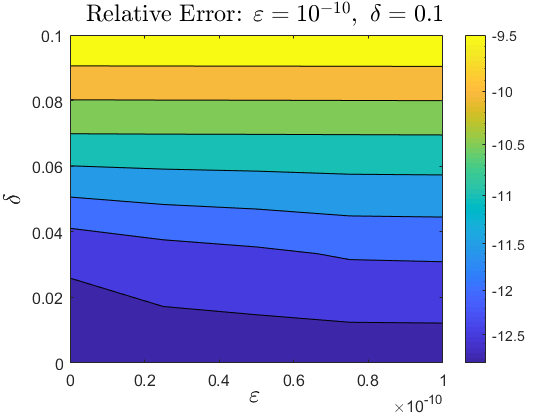
\includegraphics[width=7.6cm]{sections/7_conclusions_and_future_directions/Small_Eps_Large_Delta_2.png} }}%
    \vspace{3 mm}
    \caption{A contour plot of the relative error computed with our HOPS/AWE algorithm by holding $N=M=8$ Taylor orders fixed. In Figure $34\text{(a)}$ we expand up to $\Eps = 0.1$ and $\delta = 10^{-10}$ simultaneously with $N=M=8$ Taylor orders. In Figure $34\text{(b)}$ we expand up to $\Eps = 10^{-10}$ and $\delta = 0.1$ simultaneously with $N=M=8$ Taylor orders.}%
    \label{fig:example}%
\end{figure}
\vspace{-18mm}
Supplementary testing in both the upper and lower layers confirms that our HOPS/AWE algorithm is better suited towards larger $\varepsilon$.
%\begin{flushleft}
\newline
\\
\textbf{Predictions:} Our HOPS/AWE methodology takes advantage of exact enforcement of the \gls{owc} at an artificial boundary in order to truncate the computational domain to one of finite extent. After flattening the surface, the DNOs recover information through the solution stored at the interface. We suspect that this process mitigates large perturbations of the height/slope. By following techniques developed in \cite{NichollsReitich00b,NichollsTaber06,Nicholls16b,NichollsShen08}, we intend to rigorously prove that the TFE method is analytic when $\varepsilon$ is large. Additionally, we are interested in perturbing other physical parameters in the context of layered media problems. These are discussed in the engineering literature \cite{mashayekh2018parameter,mashayekh2018parameter2}.
\section{Rayleigh Singularities}
\label{Sec: Rayleigh Singularities}
A fundamental equation in the HOPS/AWE algorithm is
$$\alpha_p^2 + (\gamma_p^q(\delta))^2 = (k^q)^2,$$
where $k^q$ represents the wavenumber, $q\in\{u,w\}$, and $\alpha=k^q\sin(\theta), \gamma=k^q\cos(\theta),$ are parameters corresponding to refraction/reflection of the incidence angle $\theta$. As shown in $\S 5.4$, a Rayleigh singularity (or Wood's anomaly) occurs when $\ualpha_p^2 = (\uk^q)^2$ for any integer $p\neq 0$. That is, if $\ugamma_p^q(\delta) =0$ for $p\neq 0$ then the Taylor series expansion of $\gamma_p^q(\delta)$ is invalid. In \cite{Nicholls16}, the author investigated changing the Taylor expansion to a Puiseux expansion \cite{basu2007algorithms}:
$$\gamma_p^q(\delta)=\sum_{m=0}^{\infty}\gamma_{p,m}^q\delta^{m+1/2}=\delta^{1/2}\sum_{m=0}^{\infty}\gamma_{p,m}^q\delta^m.$$
However, he found that this approach ran into external difficulties ($\S$6 of \cite{Nicholls16}) simplifying explicit forms of the Dirichlet and Neumann trace operators.
\newline
\\
\textbf{Predictions:} Rayleigh singularities are a central obstruction to the convergence of our HOPS/AWE algorithm. In all of our numerical tests, we select custom frequency ranges which maximize the radius of convergence of our algorithm by expanding away from the singularities (cf. $\S 5.6$). Alternative methods such as Padé summation also fail to be analytic in a neighborhood of a Rayleigh singularity. General perturbation theory provides a variety of known techniques \cite{suslov2005divergent,convfromdiv,Heinz2020,dienes1957taylor,arteca1984summation} for expanding around divergent perturbation series. We suspect that adding these techniques to our HOPS/AWE algorithm will allow us perform a series expansion of $\ugamma_p^q(\delta)$ that does not diverge when $\ugamma_p^q(\delta)=0.$
\section{Multiple Layers}
\label{Sec: Multiple Layers}

In \cite{Nicholls16b}, the author discusses how to apply our HOPS methodology in multilayered configurations. He considers a multilayered material with $M$ (finite) interfaces at 
$$z=a^{(m)}+g^{(m)}(x,y),\quad 1\leq m \leq M,$$
which are $d_x \times d_y$ periodic
$$g^{(m)}(x+d_x,y+d_y)=g^{(m)}(x,y),\quad 1\leq m \leq M,$$
separating $(M+1)$--many layers.
%\vspace{-12mm}
\begin{figure}[H]
    \centering
    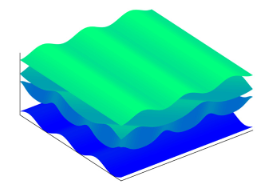
\includegraphics[width=7.6cm]{sections/7_conclusions_and_future_directions/multilayered.png}%
    \vspace{3mm}
    \caption{A five--layer problem configuration with layer interfaces $z = a^{(m)}+g^{(m)}(x).$}%
    \label{fig:example}%
\end{figure}
\vspace{-15mm}
%\begin{flushleft}
A generalization of our analyticity theorems (cf. $\S 4.5$) up to $M$ parameters is included as Theorem~$3.2$ in \cite{Nicholls16b}. For this, we consider quite general systems of linear equations of the form
%\end{flushleft}
\be
\bA(\tEps)\bV(\tEps)=\bR(\tEps),
\ee
where 
\bes
\bA(\tEps)=\sum_{\tn=0}^{\infty}\bA_{\tn}\tEps^{\tn},\quad 
\bR(\tEps) = \sum_{\tn=0}^{\infty}\bR_{\tn}\tEps^{\tn}.
\ees
The tildes represent multi--index notation \cite{Evans10}, in particular
\bes
\tEps := \begin{pmatrix} \Eps_1 \\ \vdots \\ \Eps_M \end{pmatrix},
\quad
\tn := \begin{pmatrix} n_1 \\ \vdots \\ n_M \end{pmatrix},
\ees
and the convention
\bes
\sum_{\tn=0}^{\infty} 
    A_{\tn}\ \tEps^{\tn}
  = \sum_{n_1=0}^{\infty} \cdots \sum_{n_M=0}^{\infty}
    A_{n_1,\ldots,n_M} \Eps_1^{n_1} \cdots \Eps_M^{n_M}.
\ees
As in $\S 4.5$, we seek a solution of the form
\be
\bV(\tEps)=\sum_{\tn=0}^{\infty}\bV_{\tn}\tEps^{\tn},
\ee
and from $(7.1)$ we find at order $\mathcal{O}(\tEps^{\tn})$
\bes
\bA_0\bV_{\tn}= \bR_{\tn} - \left(\sum_{\tl=0}^{\tn}\bA_{\tn-\tl}\bV_{\tl}- \bA_0\bV_{\tn}\right),
\ees
or
\be
\bV_{\tn}= \bA_0^{-1}\left\{\bR_{\tn} - \left(\sum_{\tl=0}^{\tn}\bA_{\tn-\tl}\bV_{\tl}- \bA_0\bV_{\tn}\right)\right\}.
\ee
The above notation represents multi--indices in the form
\bes
\sum_{\tl=0}^{\tn}\bA_{\tn-\tl}\bV_{\tl} = \sum_{\ell_1=0}^{n_1}\cdots \sum_{\ell_M=0}^{n_M}
    \bA_{n_1-\ell_1,\ldots,n_M-\ell_M} \bV_{\ell_1,\ldots,\ell_m},  
\ees
where $\tn=(n_1,\ldots,n_M),$ $\tl=(\ell_1,\ldots,\ell_M),$ and $0=(0,\ldots,0)$ with the convention
\bes
\tn \geq 0 \iff n_1\geq 0,\ldots,n_M\geq 0, \quad\tl \geq 0 \iff \ell_1\geq 0,\ldots,\ell_M\geq 0.
\ees
With these, we can extend our existence theorem (Theorem $4.5.1$) to $M$ parameters.
\begin{theorem}
\label{Thm:AVR}
Given two Banach spaces, $X$ and $Y$, suppose that:
\begin{enumerate}[label={\upshape[\arabic*]}]
\item $\bR_{\tn} \in Y$ for all $\tn \geq 0$,
  and there exist $M$--multi--indexed constants $C_R > 0$, $B_R > 0$,
  \bes
  C_R = \begin{pmatrix} C_{R,1} \\ \vdots \\ C_{R,M} \end{pmatrix},
  \quad
  B_R^{\tn} = \begin{pmatrix} B_{R,1}^{n_1} \\ \vdots \\ 
  B_{R,M}^{n_M} \end{pmatrix},
  \ees
  such that
  \bes
  \Norm{\bR_{\tn}}{Y} \leq C_R B_R^{\tn},
  \ees
\item $\bA_{\tn}: X \rightarrow Y$ for all
  $\tn \geq 0$, and there exist $M$--multi--indexed
  constants $C_A > 0$, $B_A > 0$ such that
  \bes
  \Norm{\bA_{\tn}}{X \rightarrow Y} \leq C_A B_A^{\tn},
  \ees
\item $\bA_0^{-1}: Y \rightarrow X$, and there 
  exists a constant $C_e > 0$ such that
  \bes
  \Norm{\bA_0^{-1}}{Y \rightarrow X} \leq C_e.
  \ees  
\end{enumerate}
Then the equation $(7.1)$ has a unique solution,
\be
\label{Eqn:V:Exp:Multi}
\bV(\tEps) = \sum_{\tn=0}^{\infty} \bV_{\tn} \tEps^{\tn},
\ee
and there exist $M$--multi--indexed constants $C_V > 0$ and $B_V > 0$ such that
\bes
\Norm{\bV_{\tn}}{X} \leq C_V B_V^{\tn},
\ees
for all $\tn \geq 0$ and any
\bes
C_V \geq 2 C_e C_R,
\quad
B_V \geq \max \left\{ B_R, 2 B_A, 2^{M+1} C_e C_A B_A \right\},
\ees
enforced componentwise. This implies that, for any $M$--multi--indexed constant
$0 \leq \tilde{\rho} < 1$, 
$(7.4)$, converges for all $\tEps$ such that
$B \tEps < \tilde{\rho}$, i.e., $\tEps < \tilde{\rho}/B$.
\end{theorem}
\begin{remark}
Our proof strategy is a form of multidimensional induction where given a statement $\bP(n_1, n_2, n_3, ..., n_M)$ for some $M\in \mathbb{N}$, we will show that $\forall n_1, n_2,\ldots, n_M \geq 0$, $\bP(n_1, n_2, n_3, ..., n_M)$ is true by inducting on $n_M$. We will follow the steps outlined below.
\begin{enumerate}
\item Establish $\bP(0,\ldots,n_j,\ldots,0)$ for all $1 \leq j < M$ and $n_1,\ldots,n_j \geq 0.$
\item Given $\bP(n_1,n_2,\ldots,n_j,\ldots,0)$ for all $1 \leq j < M$ and $n_1,\ldots,n_j \geq 0$, establish $\bP(n_1,n_2,\ldots,\bar{n}_j,\ldots,0)$. This can be accomplished through the two steps below.
\begin{enumerate}
    \item Establish $\bP(0,\ldots,\bar{n}_j,\ldots,0)$ for all $\bar{n}_j \geq 0$ (where the hypothesis in $[2]$ gives the required case for $n_j < \bar{n}_j$).
    \item Given  $\bP(n_1,n_2,\ldots,\bar{n}_j,\ldots,0)$ for all $1 \leq j < M$ and $n_1 < \bar{n}_1,  n_2 < \bar{n}_2,\ldots, $ $n_{j-1}  < \bar{n}_{j-1}$ and $\bar{n}_j\geq 0$, establish $\bP(\bar{n}_1,\bar{n}_2,\ldots,\bar{n}_j,\ldots,0)$.
\end{enumerate}
\item Given $\bP(n_1,n_2,\ldots,n_j,n_{j+1},\ldots,0)$ for all $1 \leq j+1 < M$ and $n_1,\ldots,n_{j+1} \geq 0$, establish $\bP(n_1,n_2,\ldots,n_j,\bar{n}_{j+1},\ldots,0)$. This can be accomplished by following the two steps outlined below. 
\begin{enumerate}
    \item Establish $\bP(0,\ldots,\bar{n}_{j+1},\ldots,0)$ for all $\bar{n}_{j+1} \geq 0$ (where the hypothesis in $[3]$ gives the required case for $n_{j+1} < \bar{n}_{j+1}$).
    \item Given  $\bP(n_1,n_2,\ldots,n_j,\bar{n}_{j+1},\ldots,0)$ for all $1 \leq j+1 < M$ and  $n_1 < \bar{n}_1,  n_2 < \bar{n}_2,\ldots, n_{j} < \bar{n}_{j}$ and $\bar{n}_{j+1}\geq 0$, establish $\bP(\bar{n}_1,\bar{n}_2,\ldots,\bar{n}_j,\bar{n}_{j+1}\ldots,0)$.
\end{enumerate}
\item Given $\bP(n_1,n_2,\ldots,n_{M-1},n_M)$ for all $n_1,n_2,\ldots,n_{M-1} \geq 0$ and $n_M < \bar{n}_M$, establish $\bP(n_1,n_2,\ldots,n_{M-1},\bar{n}_M)$. This can be accomplished by the two steps below (the base cases are handled through $[2]$ and $[3]$).
\begin{enumerate}
    \item Establish $\bP(0,\ldots,\bar{n}_{M})$ for $\bar{n}_{M} \geq 0$ (where the hypothesis in $[4]$ handles the required case for  $n_{M} < \bar{n}_{M}$).
    \item Given $\bP(n_1,n_2,\ldots,n_{M-1},\bar{n}_M)$ for all $n_1 < \bar{n}_1, n_2 < \bar{n}_2, \ldots n_{M-1} < \bar{n}_{M-1}$ and $\bar{n}_M \geq 0$, establish $\bP(\bar{n}_1,\bar{n}_2,\ldots,\bar{n}_{M-1},\bar{n}_M)$.
\end{enumerate}
\end{enumerate}

\end{remark}

\begin{proof}{[Theorem 7.4.1]} As with $\tEps$ and $\tn$, we represent $\tilde{\rho}$ by
\bes
\tilde{\rho} := \begin{pmatrix} \rho_1 \\ \vdots \\ \rho_M \end{pmatrix}.
\ees
As before, we will work by induction and consider the general case for finite $M>0$ where we want to establish
\bes
\norm{\bV_{n_1,\ldots,n_M}}_X \leq C_{V,1}\ldots C_{V,M} B_{V,1}^{n_1}\ldots B_{V,M}^{n_M}, \quad \forall n_1,\ldots,n_M\geq 0.
\ees
We prove this via an induction on $n_M$. The base case $n_1,n_2,\ldots, n_{j-1},n_{j+1},\ldots,$ $n_M=0$ and $1 \leq j < M$:
\bes
\norm{\bV_{0,\ldots,n_j,\ldots,0}}_X \leq C_{V,j} B_{V,j}^{n_j}, \quad \forall n_j\geq 0,
\ees
has previously been established by Theorem $4.5.1$ where $\tEps = \Eps_j$ and $\delta=0$. We now assume
\bes
\norm{\bV_{n_1,\ldots,n_j,\ldots,0}}_X \leq  C_{V,1}\ldots C_{V,j}B_{V,1}^{n_1}\ldots B_{V,j}^{n_j}, ~~ \forall n_1,\ldots,n_{j-1}\geq 0,~~ \forall n_j < \bar{n}_j,~~ 1 \leq j < M,
\ees
and seek
\bes
\norm{\bV_{n_1,\ldots,\bar{n}_j,\ldots,0}}_X \leq  C_{V,1}\ldots C_{V,j}B_{V,1}^{n_1}\ldots B_{V,j}^{\bar{n}_j}, ~~ \forall n_1,\ldots,n_{j-1}\geq 0.
\ees
This can be obtained through a chain of $(M-1)$ inductions on $n_1,\ldots,n_j$ where $1 \leq j < M$. For simplicity, we will show what happens in the arbitrary case $n_j$. The base case $n_1,\ldots,n_{j-1}=0$:
\bes
\norm{\bV_{0,\ldots,\bar{n}_j,\ldots,0}}_X \leq  C_{V,j}B_{V,j}^{\bar{n}_j}, \quad \forall \bar{n}_j \geq 0,
\ees
is established by Theorem $4.5.1$ where $\tEps = \Eps_j$ and $\delta=0$. Therefore, we assume
\begin{align*}
\norm{\bV_{n_1,\ldots,\bar{n}_j,\ldots,0}}_X \leq  C_{V,1}\ldots C_{V,j}B_{V,1}^{n_1}\ldots B_{V,j}^{\bar{n}_j},~~\forall n_1  &< \bar{n}_1,\ldots, n_{j-1} < \bar{n}_{j-1},~~ \forall \bar{n}_j \geq 0,\\&~ 1 \leq j < M,
\end{align*}
and seek
\bes
\norm{\bV_{\bar{n}_1,\ldots,\bar{n}_j,\ldots,0}}_X \leq  C_{V,1}\ldots C_{V,j}B_{V,1}^{\bar{n}_1}\ldots B_{V,j}^{\bar{n}_j}.
\ees
Recalling $\tn=(n_1,\ldots,n_j)$ and  $\tl=(\ell_1,\ldots,\ell_j)$, we define
\be
{\sum_{\tl=0}^{\tn}}^{*}\bA_{\tn-\tl}\bV_{\tl} := \sum_{\tl=0}^{\tn}\bA_{\tn-\tl}\bV_{\tl} - \bA_0\bV_{\tn},
\ee
and apply $(7.3),(7.5)$ and the mapping properties of $\bA_{0}^{-1}$ to find
\bes
\norm{\bV_{\bar{n}_1,\ldots,\bar{n}_j,\ldots,0}}_X\leq C_e\left\{\norm{\bR_{\bar{n}_1,\ldots,\bar{n}_j}}_Y + {\sum_{\tl=0}^{\tn}}^{*}\norm{\bA_{\tn-\tl}\bV_{\tl}}_Y\right\}.
\ees
Using the estimates on $\bR_{n_1,\ldots,n_j}$ and $\bA_{n_1,\ldots,n_j}$ (for all $n_1,\ldots,n_j$) and $\bV_{n_1,\ldots,n_j}$ $(n_1 < \bar{n}_1, \ldots, n_j < \bar{n}_j)$ we have
\begin{align*}
\norm{\bV_{\bar{n}_1,\ldots,\bar{n}_j,\ldots,0}}_X &\leq
C_e\Bigg\{C_{R,1}\ldots C_{R,j}B_{R,1}^{\bar{n}_1}\ldots B_{R,j}^{\bar{n}_j} + {\sum_{\tl=0}^{\tn}}^{*}C_{A,1}\ldots C_{A,j}B_{A,1}^{\bar{n}_1-\ell_1}\ldots B_{A,j}^{\bar{n}_j-\ell_j}\\ & \qquad \qquad \qquad \qquad \qquad \qquad \qquad \qquad \times
C_{V,1}\ldots C_{V,j}B_{V,1}^{\ell_1}\ldots B_{V,j}^{\ell_j}\Bigg\} \\& =
C_eC_{R,1}\ldots C_{R,j}B_{R,1}^{\bar{n}_1}\ldots B_{R,j}^{\bar{n}_j} + C_eC_{A,1}\ldots C_{A,j}C_{V,1}\ldots C_{V,j} \\&
~~ \times \left(\frac{B_{A,1}}{B_{V,1}}\right)B_{V,1}^{\bar{n}_1}\cdots \left(\frac{B_{A,j}}{B_{V,j}}\right)B_{V,j}^{\bar{n}_j}{\sum_{\tl=0}^{\tn}}^{*}
\left(\frac{B_{A,1}}{B_{V,1}}\right)B_{V,1}^{\bar{n}_1-\ell_1-1}\cdots \\& ~~ \times
\left(\frac{B_{A,j}}{B_{V,j}}\right)B_{V,j}^{\bar{n}_j-\ell_j-1} \\& \leq
C_eC_{R,1}\ldots C_{R,j}B_{V,1}^{\bar{n}_1}\ldots B_{V,j}^{\bar{n}_j} + C_eC_{A,1}\ldots C_{A,j}C_{V,1}\ldots C_{V,j} \\& ~~ \times
\left(\frac{B_{A,1}}{B_{V,1}}\right)B_{V,1}^{\bar{n}_1}\cdots\left(\frac{B_{A,j}}{B_{V,j}}\right)B_{V,j}^{\bar{n}_j}\left(\frac{1}{1-1/2}\right)^j,
\end{align*}
if $B_{A,k}/B_{V,k} \leq 1/2$, $k=1,\ldots,j$ (implying $B_{V,k} \geq 2B_{A,k}$). We are done if we demand that
\bes
B_{V,k} \geq B_{R,k}, \quad C_eC_{R,k} \leq C_{V,k}/2, \quad 2^jC_eC_{A,k}C_{V,k}(B_{A,k}/B_{V,k}) \leq 
C_{V,k}/2.
\ees
This can be realized if
\bes
C_{V,k} \geq 2C_eC_{R,k}, \quad
B_{V,k} \geq \max\left\{B_{R,k},2B_{A,k},2^{j+1}C_eC_{A,k}B_{A,k}\right\}.
\ees
We then assume
\begin{align*}
\norm{\bV_{n_1,\ldots,n_{j+1},\ldots,0}}_X \leq  C_{V,1}\ldots C_{V,j+1}B_{V,1}^{n_1}\ldots B_{V,j+1}^{n_{j+1}}, ~~ &\forall n_1,\ldots,n_j\geq 0,~~ \forall n_{j+1} < \bar{n}_{j+1},\\&~~ 1 \leq j < M,
\end{align*}
and seek
\bes
\norm{\bV_{n_1,\ldots,\bar{n}_{j+1},\ldots,0}}_X \leq  C_{V,1}\ldots C_{V,j+1}B_{V,1}^{n_1}\ldots B_{V,j+1}^{\bar{n}_{j+1}}, ~~ \forall n_1,\ldots,n_{j}\geq 0.
\ees
As before, this can be obtained through a chain of $M$ inductions on $n_1,\ldots,n_{j+1}$ where $1 \leq j < M$. For simplicity, we will show what happens in the arbitrary case $n_{j+1}$. The base case $n_1,\ldots,n_{j}=0$:
\bes
\norm{\bV_{0,\ldots,\bar{n}_{j+1},\ldots,0}}_X \leq  C_{V,j+1}B_{V,j+1}^{\bar{n}_{j+1}}, \quad \forall \bar{n}_{j+1} \geq 0,
\ees
is established by Theorem $4.5.1$ where $\tEps = \Eps_{j+1}$ and $\delta=0$. Therefore, we assume
\begin{align*}
\norm{\bV_{n_1,\ldots,\bar{n}_{j+1},\ldots,0}}_X \leq  C_{V,1}\ldots C_{V,j+1}B_{V,1}^{n_1}\ldots B_{V,j+1}^{\bar{n}_{j+1}},~~\forall n_1  &< \bar{n}_1,\ldots, n_{j} < \bar{n}_{j},~~ \forall \bar{n}_{j+1} \geq 0,\\&~ 1 \leq j < M,
\end{align*}
and seek
\bes
\norm{\bV_{\bar{n}_1,\ldots,\bar{n}_{j+1},\ldots,0}}_X \leq  C_{V,1}\ldots C_{V,j+1}B_{V,1}^{\bar{n}_1}\ldots B_{V,j+1}^{\bar{n}_{j+1}}.
\ees
In this scenario, $\tn=(n_1,\ldots,n_{j+1})$ and  $\tl=(\ell_1,\ldots,\ell_{j+1}),$ so we apply $(7.3),(7.5)$ and the mapping properties of $\bA_{0}^{-1}$ to find
\bes
\norm{\bV_{\bar{n}_1,\ldots,\bar{n}_{j+1},\ldots,0}}_X\leq C_e\left\{\norm{\bR_{\bar{n}_1,\ldots,\bar{n}_{j+1}}}_Y + {\sum_{\tl=0}^{\tn}}^{*}\norm{\bA_{\tn-\tl}\bV_{\tl}}_Y\right\}.
\ees
Using the estimates on $\bR_{n_1,\ldots,n_{j+1}}$ and $\bA_{n_1,\ldots,n_{j+1}}$ (for all $n_1,\ldots,n_{j+1}$) and $\bV_{n_1,\ldots,n_{j+1}}$ $(n_1 < \bar{n}_1, \ldots, n_{j+1} < \bar{n}_{j+1})$ we have
\begin{align*}
\norm{\bV_{\bar{n}_1,\ldots,\bar{n}_{j+1},\ldots,0}}_X &\leq
C_e\Bigg\{C_{R,1}\ldots C_{R,{j+1}}B_{R,1}^{\bar{n}_1}\ldots B_{R,{j+1}}^{\bar{n}_{j+1}} + {\sum_{\tl=0}^{\tn}}^{*}C_{A,1}\ldots C_{A,{j+1}}B_{A,1}^{\bar{n}_1-\ell_1}\ldots \\ & \qquad \qquad \qquad \qquad \qquad \quad \times
B_{A,{j+1}}^{\bar{n}_{j+1}-\ell_{j+1}}C_{V,1}\ldots C_{V,{j+1}}B_{V,1}^{\ell_1}\ldots B_{V,{j+1}}^{\ell_{j+1}}\Bigg\} \\& =
C_eC_{R,1}\ldots C_{R,{j+1}}B_{R,1}^{\bar{n}_1}\ldots B_{R,{j+1}}^{\bar{n}_{j+1}} + C_eC_{A,1}\ldots C_{A,{j+1}}C_{V,1}\ldots C_{V,{j+1}} \\&
~~ \times \left(\frac{B_{A,1}}{B_{V,1}}\right)B_{V,1}^{\bar{n}_1}\cdots \left(\frac{B_{A,{j+1}}}{B_{V,{j+1}}}\right)B_{V,{j+1}}^{\bar{n}_{j+1}}{\sum_{\tl=0}^{\tn}}^{*}
\left(\frac{B_{A,1}}{B_{V,1}}\right)B_{V,1}^{\bar{n}_1-\ell_1-1}\cdots \\& ~~ \times
\left(\frac{B_{A,{j+1}}}{B_{V,{j+1}}}\right)B_{V,{j+1}}^{\bar{n}_{j+1}-\ell_{j+1}-1} \allowdisplaybreaks\\& \leq
C_eC_{R,1}\ldots C_{R,{j+1}}B_{V,1}^{\bar{n}_1}\ldots B_{V,{j+1}}^{\bar{n}_{j+1}} + C_eC_{A,1}\ldots C_{A,{j+1}}C_{V,1}\ldots C_{V,{j+1}} \\& ~~ \times
\left(\frac{B_{A,1}}{B_{V,1}}\right)B_{V,1}^{\bar{n}_1}\cdots\left(\frac{B_{A,{j+1}}}{B_{V,{j+1}}}\right)B_{V,{j+1}}^{\bar{n}_{j+1}}\left(\frac{1}{1-1/2}\right)^{j+1},
\end{align*}
if $B_{A,t}/B_{V,t} \leq 1/2$, $t=1,\ldots,j+1$ (implying $B_{V,t} \geq 2B_{A,t}$). We are done if we demand that
\bes
B_{V,t} \geq B_{R,t}, \quad C_eC_{R,t} \leq C_{V,t}/2, \quad 2^{j+1}C_eC_{A,t}C_{V,t}(B_{A,t}/B_{V,t}) \leq 
C_{V,t}/2.
\ees
This can be realized if
\bes
C_{V,t} \geq 2C_eC_{R,t}, \quad
B_{V,t} \geq \max\left\{B_{R,t},2B_{A,t},2^{j+2}C_eC_{A,t}B_{A,t}\right\}.
\ees
To complete the general case for finite $M>0$, we assume
\bes
\norm{\bV_{n_1,\ldots,n_M}}_X \leq  C_{V,1}\ldots C_{V,M}B_{V,1}^{n_1}\ldots B_{V,M}^{n_M}, ~~ \forall n_1,\ldots,n_{M-1}\geq 0,~~ \forall n_M < \bar{n}_M,
\ees
and seek
\bes
\norm{\bV_{n_1,\ldots,\bar{n}_M}}_X \leq  C_{V,1}\ldots C_{V,M}B_{V,1}^{n_1}\ldots B_{V,M}^{\bar{n}_M}, ~~ \forall n_1,\ldots,n_{M-1}\geq 0.
\ees
The base case $n_1,n_2,\ldots,n_{M-1}=0$:
\bes
\norm{\bV_{0,\ldots,\bar{n}_M}}_X \leq  C_{V,M}B_{V,M}^{\bar{n}_M}, \quad \forall \bar{n}_M \geq 0,
\ees
has previously been established by Theorem $4.5.1$ where $\tEps = \Eps_M$ and $\delta =0$. Finally, we assume
\begin{align*}
\norm{\bV_{n_1,\ldots,n_{M-1},\bar{n}_M}}_X \leq  C_{V,1}\ldots C_{V,M}B_{V,1}^{n_1}\ldots B_{V,M}^{\bar{n}_M},~~~&\forall n_1  < \bar{n}_1,\ldots, n_{M-1} < \bar{n}_{M-1},\\&~~~~ \forall \bar{n}_M \geq 0,
\end{align*}
and seek
\bes
\norm{\bV_{\bar{n}_1,\ldots,\bar{n}_{M-1},\bar{n}_M}}_X \leq  C_{V,1}\ldots C_{V,M}B_{V,1}^{\bar{n}_1}\ldots B_{V,M}^{\bar{n}_M}.
\ees
In this case, $\tn=(n_1,\ldots,n_M)$ and  $\tl=(\ell_1,\ldots,\ell_M),$ so we apply $(7.3),(7.5)$ and the mapping properties of $\bA_{0}^{-1}$ to find
\bes
\norm{\bV_{\bar{n}_1,\ldots,\bar{n}_M}}_X\leq C_e\left\{\norm{\bR_{\bar{n}_1,\ldots,\bar{n}_M}}_Y + {\sum_{\tl=0}^{\tn}}^{*}\norm{\bA_{\tn-\tl}\bV_{\tl}}_Y\right\}.
\ees
Using the estimates on $\bR_{n_1,\ldots,n_M}$ and $\bA_{n_1,\ldots,n_M}$ (for all $n_1,\ldots,n_M$) and $\bV_{n_1,\ldots,n_M}$ $(n_1 < \bar{n}_1, \ldots, n_M < \bar{n}_M)$ we have
\vspace{-1.5mm}
\begin{align*}
\norm{\bV_{\bar{n}_1,\ldots,\bar{n}_M}}_X &\leq
C_e\Bigg\{C_{R,1}\ldots C_{R,M}B_{R,1}^{\bar{n}_1}\ldots B_{R,M}^{\bar{n}_M} + {\sum_{\tl=0}^{\tn}}^{*}C_{A,1}\ldots C_{A,M}B_{A,1}^{\bar{n}_1-\ell_1}\ldots B_{A,M}^{\bar{n}_M-\ell_M}\\ & \qquad \qquad \qquad \qquad \qquad \qquad \qquad \qquad \times
C_{V,1}\ldots C_{V,M}B_{V,1}^{\ell_1}\ldots B_{V,M}^{\ell_M}\Bigg\} \\& =
C_eC_{R,1}\ldots C_{R,M}B_{R,1}^{\bar{n}_1}\ldots B_{R,M}^{\bar{n}_M} + C_eC_{A,1}\ldots C_{A,M}C_{V,1}\ldots C_{V,M} \\& 
~~ \times \left(\frac{B_{A,1}}{B_{V,1}}\right)B_{V,1}^{\bar{n}_1}\cdots \left(\frac{B_{A,M}}{B_{V,M}}\right)B_{V,M}^{\bar{n}_M}{\sum_{\tl=0}^{\tn}}^{*}
\left(\frac{B_{A,1}}{B_{V,1}}\right)B_{V,1}^{\bar{n}_1-\ell_1-1}\cdots \\& \allowdisplaybreaks~~ \times
\left(\frac{B_{A,M}}{B_{V,M}}\right)B_{V,M}^{\bar{n}_M-\ell_M-1} \\&  \leq
C_eC_{R,1}\ldots C_{R,M}B_{V,1}^{\bar{n}_1}\ldots B_{V,M}^{\bar{n}_M} + C_eC_{A,1}\ldots C_{A,M}C_{V,1}\ldots C_{V,M} \\& ~~ \times
\left(\frac{B_{A,1}}{B_{V,1}}\right)B_{V,1}^{\bar{n}_1}\cdots\left(\frac{B_{A,M}}{B_{V,M}}\right)B_{V,M}^{\bar{n}_M}\left(\frac{1}{1-1/2}\right)^M,
\end{align*}
if $B_{A,i}/B_{V,i} \leq 1/2$, $i=1,\ldots,M$ (implying $B_{V,i} \geq 2B_{A,i}$). We are done if we demand that
\bes
B_{V,i} \geq B_{R,i}, \quad C_eC_{R,i} \leq C_{V,i}/2, \quad 2^MC_eC_{A,i}C_{V,i}(B_{A,i}/B_{V,i}) \leq 
C_{V,i}/2.
\ees
This can be realized if
\bes
C_{V,i} \geq 2C_eC_{R,i}, \quad
B_{V,i} \geq \max\left\{B_{R,i},2B_{A,i},2^{M+1}C_eC_{A,i}B_{A,i}\right\}.
\ees
\end{proof}
Using a similar approach in conjunction with the analysis in Chapters $2$ and $3$, we predict a more general form of Theorems $2.9.2$ and $3.8.1$ exists, which would establish the analyticity of the transformed field with respect to any finite $M > 0$ perturbation parameters.
\vspace{1mm}
\begin{conjecture} 
\label{Conj:u,w:Anal:n:n_m}
Given any integer $s \geq 0$, if $f \in C^{s+2}([0,d])$ and 
$U_{\tilde{n}} \in H^{s+3/2}([0,d])$, $W_{\tilde{n}}\in H^{s+3/2}([0,d])$ such that
\bes
\|U_{\tilde{n}}\|_{H^{s+3/2}} \le K_U B_U^{\tn} , \quad
\|W_{\tilde{n}}\|_{H^{s+3/2}} \le K_W B_W^{\tn} ,
\ees
for constants $K_U, K_W>0$ and $M$--multi--indexed constants $B_U, B_W > 0$, then 
$u_{\tn} \in H^{s+2}([0,d]\times[0,a])$, $w_{\tn}\in H^{s+2}([0,d]\times[-b,0])$ and
\bes
\label{Eqn:u,w:Est:n:n_m}
\|u_{\tn}\|_{H^{s+2}} \le K B^{\tn}, \quad
\|w_{\tn}\|_{H^{s+2}} \le \tilde{K}\tilde{B}^{\tn} ,
\ees
for constants $K,\tilde{K}> 0$ and $M$--multi--indexed constants $B ,\tilde{B}>0$.
\end{conjecture}
\vspace{1mm}
Analogously, a similar procedure would establish a more general form of Theorems $2.10.2$ and $3.9.2$ for the analyticity of the DNOs for any finite $M>0$ perturbation parameters.
\vspace{1mm}
\begin{conjecture} 
\label{Thm:G,J:Anal:n:n_m}
Given any integer $s \geq 0$, if $f \in C^{s+2}([0,d])$ and 
$U_{\tn} \in H^{s+3/2}([0,d])$, $W_{\tn} \in H^{s+3/2}([0,d])$ such that
\bes
\SobNorm{U_{\tn}}{s+3/2} \leq K_U B_U^{\tn}, \quad
\SobNorm{W_{\tn}}{s+3/2} \leq K_W B_W^{\tn},
\ees
for constants $K_U,K_W> 0$ and $M$--multi--indexed constants $B_U, B_W > 0$, then $G_{\tn} \in H^{s+1/2}([0,d])$, $J_{\tn} \in H^{s+1/2}([0,d])$ and
\bes
\label{Eqn:G,J:Est:n:n_m} 
\|G_{\tn}\|_{H^{s+1/2}} \le \tilde{K}\tilde{B}^{\tn}, \quad
\|J_{\tn}\|_{H^{s+1/2}} \le \dbtilde{K} \dbtilde{B}^{\tn},
\ees
for constants $\tilde{K},\dbtilde{K}  > 0$ and $M$--multi--indexed constants $\tilde{B},\dbtilde{B}>0$.
\end{conjecture}
\vspace{1mm}
Upon proving these, one has two key ingredients to the more general version of Theorem $4.6.1$ which establishes the existence and uniqueness of solutions to a system of partial differential equations with respect to $M$ perturbation parameters.
\vspace{1mm}
\begin{conjecture} 
\label{Conj:Main}
Given an integer $s \geq 0$, if $f \in C^{s+2}([0,d])$ then the 
equation $(7.1)$ has a unique solution, $(7.4)$,
and there exist a constant $C > 0$ and $M$--multi--indexed constants $B>0$ such that
\bes
\Norm{\bV_{\tn}}{X^s} \leq C B^{\tn},
\ees
for all $\tn \geq 0$.  This implies that for any $M$--multi--indexed constant
$0 \leq \tilde{\rho} < 1$, $(7.4)$, converges for all $\tEps$ such that
$B \tEps < \tilde{\rho}$, i.e., $\tEps < \tilde{\rho}/B$.
\end{conjecture}
\vspace{1mm}
\textbf{Predictions:} In application oriented fields such as signal processing or sea ice modeling, practitioners work with  multiple frequencies \cite{qiu2005high,bosse1995model,zhao2009multi,blanchard2021high} at short or long wavelengths. Also, as depicted in Figure $35$, the grating surface could have $M$ different layers \cite{imperatore2017perturbation} with distinct values of $g_j(x)=\Eps f_j(x),~j=1,\ldots, M$. A proof of Conjecture $7.4.4$ would enable the freedom to enforce any number of perturbation parameters and obtain an analytic solution. Given the widespread availability of parallel computing resources coupled with additional perturbation parameters associated with elastic media, we believe that future research will force hundreds or even thousands of distinct perturbation parameters, all of which should yield an analytic solution.
\section{Parallel Programming}
\setcounter{section}{5}
\label{Sec: Parallel Programming}

In the case of multiple layered interfaces, we need to compute intermediate DNOs for up to $M$ layers. This will greatly increase the computational cost and execution time of our HOPS/AWE algorithm and we suspect that it will be necessary to introduce parallel programming techniques to offset the computational expense. In the context of the \gls{oe} method, preliminary work \cite{fang2015operator} has been completed in C\texttt{++} to parallelize the computation of Navier's equations \cite{BillinghamKing00,achenbach2012wave}. These techniques can be adapted to the TFE method through the choice of OpenMP \cite{chandra2001parallel}, MPI \cite{snir1998mpi}, or CUDA \cite{sanders2010cuda}.
\newline
\\
\textbf{Predictions:} In two or three dimensions, our HOPS code is robust, efficient and has a runtime less than an hour. A local machine with an Intel Core i$5$ CPU, $8$GB of RAM, and Windows $10$ OS completed almost every simulation in this thesis in less than thirty minutes. However, with ten to one hundred layer configurations, we suspect that many simulations will take on the order of weeks or even months. As a result, it will be necessary to parallelize our Matlab code in a compiled programming language such as C or  C\texttt{++}.

\section{Alternatives to DNOs}
\label{Sec: Alternatives to DNOs}
In Chapter $4$ we wrote our scattering problem as a linear system
\bes
\bA \bV = \bR,
\ees
where, upon expanding $\{\bA,\bV,\bR\}$ in both $\varepsilon$ and $\delta$, we arrived at the flat--interface solution $\bA_{0,0}\bV_{0,0}=\bR_{0,0}$
at order $\mathcal{O}(\varepsilon^0,\delta^0)$. We then saw it was necessary to invert
\bes
\bA_{0,0} = \begin{pmatrix}I & -I\\
-G_{0,0} & -\tau^2J_{0,0}\end{pmatrix}, 
\ees
which features the two DNOs, $G_{0,0}$ and $J_{0,0}$, in order to show the existence and uniqueness of solutions. A primary feature of all HOPS schemes is the inversion of a single, sparse operator $\bA_{0,0}$ through the use of DNOs. However, one may ponder if a different technique could produce a more competitive algorithm that is comparable to our HOPS/AWE algorithm (or even better). Is it absolutely necessary to pass in transformed field data in order to efficiently compute and recover internal information stored at the grating surface?
\\
\newline
\textbf{Predictions:} A primary advantage of our HOPS/AWE scheme is that for every perturbation order, it is only necessary to invert a single sparse operator corresponding to a flat--interface, order--zero approximation. There are a number of competing approaches in general perturbation theory within the context of layered media problems. In regards to electromagnetic wave scattering, Galerkin and boundary element methods are discussed in \cite{escapil2020helmholtz,silva2017quantifying,nakata1990boundary,elschner2012optimization,rathsfeld2006} and a high--order perturbation approach based on boundary integral equations in \cite{dolz2020higher}. High--order schemes for linear waves can be computed using level set methods \cite{sethian1999level} and fast marching methods, as well as other methods involving domain decomposition \cite{el2004comparing,benamou1997domain,larsson1999domain,gong2021convergence,perez2018domain,chan1994domain}. A holistic evaluation of these competing methods could potentially improve our HOPS/AWE algorithm if we found a faster method of inverting linear operators without the use of DNOs.
\section{Computational Complexity}
\label{Sec: Computational Complexity}

One of the fundamental reasons for developing our HOPS/AWE algorithm is its advantageous computational complexity for problems within its domain of applicability.
In comparison with other classical methods, our HOPS/AWE approach has several advantages for computing quantities such as the Reflectivity Map, $R=R(\varepsilon,\delta)$. To demonstrate this we begin
by fixing the problem of computing $R$ for $N_{\Eps}$ many values of 
$\Eps$ and $N_{\delta}$ many values of $\delta$.

In the case of computing the DNOs $G$ and $J$, we recall from $\S 2.11$ and $\S 3.10$ that our HOPS/AWE algorithm requires
$N_x \times N_z$ unknowns at every perturbation order, $(n,m)$, corresponding to
the $N_x$ equally--spaced gridpoints in the lateral direction and the $N_z + 1$ collocation points in the vertical dimension. In $\S 4.5$ we saw that we could write our scattering problem as $\bA(\Eps,\delta) \bV(\Eps,\delta) = \bR(\Eps,\delta)$ where
\bes
    \bA(\Eps,\delta)=\sumn \summ \bA_{n,m}\Eps^n\delta^m, \quad \bR(\Eps,\delta) = \sumn \summ \bR_{n,m}\Eps^{n}\delta^m,
\ees
and
\bes
\label{Eqn:Soln:Two_Param_Append}
\bV(\Eps,\delta) = \sumn \summ \bV_{n,m}\Eps^{n}\delta^m.
\ees
At order $\mathcal{O}(\Eps^n,\delta^m)$ this becomes
\begin{align}
\begin{split}
\bA_{0,0}\bV_{n,m}=&~\bR_{n,m}-\sum_{\ell=0}^{n-1}\bA_{n-\ell,0}\bV_{\ell,m}-\sum_{r=0}^{m-1}\bA_{0,m-r}\bV_{n,r}\\&
-\sum_{\ell=0}^{n-1}\sum_{r=0}^{m-1}\bA_{n-\ell,m-r}\bV_{\ell,r}.
\end{split}
\end{align}
A careful study of $(7.6)$
reveals that the computational complexity of forming the
right--hand side at order $(n,m)$ is
\bes
\BigOh{n m N_x \log(N_x) N_z \log(N_z)}.
\ees
Inverting the operator $\bA_{0,0}$ has complexity $\BigOh{N_x \log(N_x) N_z \log(N_z)}$
so the full cost of computing the $\bV_{n,m}$, 
$\{ 0 \leq n \leq N, 0 \leq m \leq M \}$, is
\bes
\BigOh{N^2 M^2 N_x \log(N_x) N_z \log(N_z)}.
\ees
Once these coefficients are recovered, the cost of summing the series in 
$(\Eps,\delta)$ is minimal, provided it is done in an efficient manner 
(e.g., by Horner's rule \cite{BurdenFaires,AtkinsonHan01}). Our algorithm then 
requires an additional $\BigOh{N_{\Eps} N_{\delta}}$ steps to sum 
over every value of $(\Eps,\delta)$, therefore the full cost of 
computing the Reflectivity Map by our HOPS/AWE method is
\be
\BigOh{N^2 M^2 N_x \log(N_x) N_z \log(N_z) + N_{\Eps} N_{\delta}}.
\ee
In contrast, for a single $(\Eps,\delta)$ pair, a Boundary Integral Method solver with $N_x$ lateral
gridpoints requires time proportional to $\BigOh{N_x^3}$ for Gaussian elimination
to solve the resulting dense system of $N_x$ equations in $N_x$ unknowns
\cite{BurdenFaires,AtkinsonHan01,ColtonKress13}. Applying this 
$N_{\Eps} \times N_{\delta}$ times results in a total computational complexity of
\be
\BigOh{N_x^3 N_{\Eps} N_{\delta}}.
\ee
Thus, once $N_{\Eps}$ and $N_{\delta}$ become large, e.g.,

\bes
N_{\Eps} N_{\delta} > \frac{N^2 M^2 N_x \log(N_x) N_z \log(N_z)}{N_x^3},
\ees
our new algorithm becomes far more efficient. We speculate that the cost of $(7.7)$ could be reduced to
\be
\BigOh{N M \log(NM)N_x \log(N_x) N_z \log(N_z) + N_{\Eps} N_{\delta}},
\ee
provided that we develop a more efficient method of computing the $\bV_{n,m}$, 
$\{ 0 \leq n \leq N, 0 \leq m \leq M \}$, such as reducing the problem space at every step. Alternative approaches to layered media problems have also been proposed by other authors \cite{bai2004reduction,chew2005fast}, including interpolation \cite{atkins2010fast} and Green's function \cite{konno2016fast}.
\newline
\\
\textbf{Predictions:} The combination of implementing parallel programming techniques (through, e.g., OpenMP or CUDA) and reducing the problem space at every step will greatly enhance the speed and fidelity of our HOPS/AWE algorithm. Considering the natural advantage surface methods have over conventional methods, such as finite difference, finite element, and spectral element methods, we expect that our HOPS/AWE algorithm will be among the most competitive available for periodic layered media problems.
\chapter{Conclusions and Future Work}
\label{sec:conclusions_and_future_dir}

\fancyhead[LO]{\text{Chapter 7}\quad \text{Conclusions and Future Work}}

This thesis establishes a novel HOPS/AWE algorithm that is particularly well suited to simulating scattering returns for periodic media problems. Our main contribution is that of Theorem $4.6.1$ which guarantees the existence and uniqueness of solutions to a system of partial differential equations which model the interaction of linear waves in periodic layered structures with respect to multiple perturbation parameters. Through the introduction of DNOs and a change of variables based on the TFE methodology, we have shown that solutions to the Helmholtz problem are jointly analytic with respect to both interfacial and frequency perturbations. As a result, our HOPS/AWE algorithm is able to handle a variety of numerical simulations that are physically challenging in both the TE and TM polarization modes. Moreover, our extensive numerical results demonstrate the accuracy, speed, and robustness expected of all HOPS methods.


\section{Future Directions}
\label{Sec: Future Directions}
There are a wide range of improvements to both the HOPS/AWE algorithm and the proof of analyticity for linear waves in periodic layered media. Our main goals for future research are to expand the TFE method through a new proof of convergence, investigate expanding around singularities, evaluate analyticity theorems in multilayered configurations, add new parallel programming functionality, explore alternative methods to recover surface data without Dirichlet--Neumann Operators, and to reduce the execution time of the HOPS algorithm. We now summarize these six research goals and suggest predictions for future research.
\begin{enumerate}[labelsep=0ex,align=left,start=1]
    \item[\textbf{Goal 1-}] ~\textbf{Choice of Parameters: Does the geometry of the perturbation impact how large the size of the perturbation can be? }
    \item[\textbf{Goal 2-}] ~\textbf{Rayleigh Singularities: Can we build a full HOPS algorithm based on points where the Taylor expansion is invalid? }
    \item[\textbf{Goal 3-}] ~\textbf{Multiple Layers: Can we prove analyticity results when the number of layers is greater than three? Do the same theorems hold for ten or one hundred layers?} 
    \item[\textbf{Goal 4-}] ~\textbf{{Parallel Programming}: Can we implement parallel programming techniques so that our HOPS code runs on $N$ processors? }
    \item[\textbf{Goal 5-}] ~\textbf{{Alternatives to DNOs}: Do we need to use DNOs to recover surface data from information stored in the transformed field? Is there an alternative method which preserves the inversion of a single, sparse operator at the interface?   }
    \item[\textbf{Goal 6-}] ~\textbf{Computational Costs: Can we reduce the execution time per time step in our HOPS algorithm?} 
\end{enumerate}

\section{Choice of Parameters}
\label{Sec: Choice of Parameters}
Our HOPS/AWE algorithm is based on two smallness assumptions:
\begin{enumerate}
\item \text{Boundary Perturbation: $g(x)=\varepsilon f(x),$ $\varepsilon\in\mathbb R$, $\varepsilon \ll 1$,}
\vspace{-2mm}
\item \text{Frequency Perturbation: $\omega=(1+\delta)\underline{\omega}=\underline{\omega}+\delta\underline{\omega},$ $\omega\in\mathbb R$, $\delta \ll 1$,} 
\end{enumerate}
with the additional assumption that $f$ is sufficiently smooth ($f\in C^2$ \cite{NichollsReitich99,NichollsReitich03b} or even Lipschitz \cite{hu2005analyticity}). Numerical simulations show that our HOPS/AWE algorithm can handle larger perturbations of $\varepsilon$ (the height/slope) in comparison to $\delta$ (the frequency). With modest test parameters and a period of $d=2\pi$, we are able to perturb the value of $\varepsilon$ (to $\varepsilon=0.1$ or even $\varepsilon=0.2$) and still get reasonable convergence results. At a value around $\varepsilon = 10^{-4}$, our HOPS/AWE algorithm converges to machine precision provided that we sum to high enough Taylor orders.
\vspace{-13mm}
\begin{figure}[H]
    \centering
    \subfloat[\centering Large $\varepsilon$, Small $\delta$ ]{{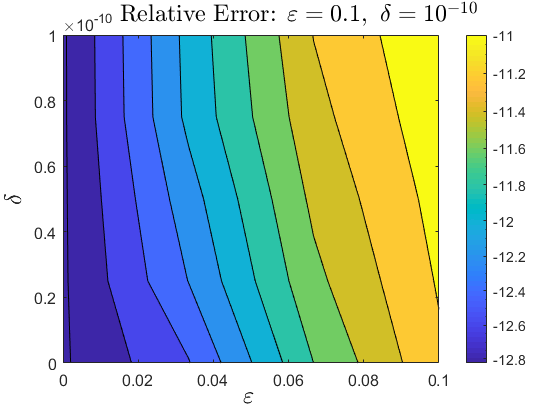
\includegraphics[width=7.6cm]{sections/7_conclusions_and_future_directions/Large_Eps_Small_Delta_2.png} }}%
    %\qquad
    \subfloat[\centering Small $\varepsilon$, Large $\delta$ ]{{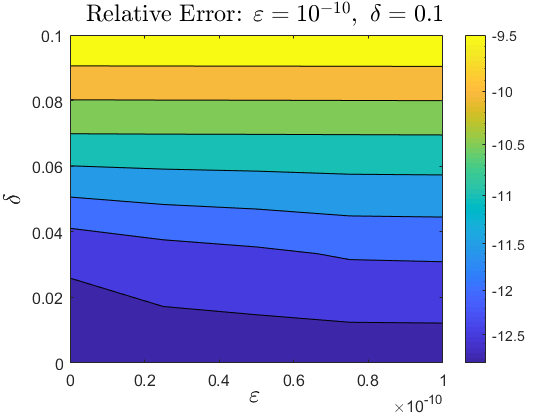
\includegraphics[width=7.6cm]{sections/7_conclusions_and_future_directions/Small_Eps_Large_Delta_2.png} }}%
    \vspace{3 mm}
    \caption{A contour plot of the relative error computed with our HOPS/AWE algorithm by holding $N=M=8$ Taylor orders fixed. In Figure $34\text{(a)}$ we expand up to $\Eps = 0.1$ and $\delta = 10^{-10}$ simultaneously with $N=M=8$ Taylor orders. In Figure $34\text{(b)}$ we expand up to $\Eps = 10^{-10}$ and $\delta = 0.1$ simultaneously with $N=M=8$ Taylor orders.}%
    \label{fig:example}%
\end{figure}
\vspace{-18mm}
Supplementary testing in both the upper and lower layers confirms that our HOPS/AWE algorithm is better suited towards larger $\varepsilon$.
%\begin{flushleft}
\newline
\\
\textbf{Predictions:} Our HOPS/AWE methodology takes advantage of exact enforcement of the \gls{owc} at an artificial boundary in order to truncate the computational domain to one of finite extent. After flattening the surface, the DNOs recover information through the solution stored at the interface. We suspect that this process mitigates large perturbations of the height/slope. By following techniques developed in \cite{NichollsReitich00b,NichollsTaber06,Nicholls16b,NichollsShen08}, we intend to rigorously prove that the TFE method is analytic when $\varepsilon$ is large. Additionally, we are interested in perturbing other physical parameters in the context of layered media problems. These are discussed in the engineering literature \cite{mashayekh2018parameter,mashayekh2018parameter2}.
\section{Rayleigh Singularities}
\label{Sec: Rayleigh Singularities}
A fundamental equation in the HOPS/AWE algorithm is
$$\alpha_p^2 + (\gamma_p^q(\delta))^2 = (k^q)^2,$$
where $k^q$ represents the wavenumber, $q\in\{u,w\}$, and $\alpha=k^q\sin(\theta), \gamma=k^q\cos(\theta),$ are parameters corresponding to refraction/reflection of the incidence angle $\theta$. As shown in $\S 5.4$, a Rayleigh singularity (or Wood's anomaly) occurs when $\ualpha_p^2 = (\uk^q)^2$ for any integer $p\neq 0$. That is, if $\ugamma_p^q(\delta) =0$ for $p\neq 0$ then the Taylor series expansion of $\gamma_p^q(\delta)$ is invalid. In \cite{Nicholls16}, the author investigated changing the Taylor expansion to a Puiseux expansion \cite{basu2007algorithms}:
$$\gamma_p^q(\delta)=\sum_{m=0}^{\infty}\gamma_{p,m}^q\delta^{m+1/2}=\delta^{1/2}\sum_{m=0}^{\infty}\gamma_{p,m}^q\delta^m.$$
However, he found that this approach ran into external difficulties ($\S$6 of \cite{Nicholls16}) simplifying explicit forms of the Dirichlet and Neumann trace operators.
\newline
\\
\textbf{Predictions:} Rayleigh singularities are a central obstruction to the convergence of our HOPS/AWE algorithm. In all of our numerical tests, we select custom frequency ranges which maximize the radius of convergence of our algorithm by expanding away from the singularities (cf. $\S 5.6$). Alternative methods such as Padé summation also fail to be analytic in a neighborhood of a Rayleigh singularity. General perturbation theory provides a variety of known techniques \cite{suslov2005divergent,convfromdiv,Heinz2020,dienes1957taylor,arteca1984summation} for expanding around divergent perturbation series. We suspect that adding these techniques to our HOPS/AWE algorithm will allow us perform a series expansion of $\ugamma_p^q(\delta)$ that does not diverge when $\ugamma_p^q(\delta)=0.$
\section{Multiple Layers}
\label{Sec: Multiple Layers}

In \cite{Nicholls16b}, the author discusses how to apply our HOPS methodology in multilayered configurations. He considers a multilayered material with $M$ (finite) interfaces at 
$$z=a^{(m)}+g^{(m)}(x,y),\quad 1\leq m \leq M,$$
which are $d_x \times d_y$ periodic
$$g^{(m)}(x+d_x,y+d_y)=g^{(m)}(x,y),\quad 1\leq m \leq M,$$
separating $(M+1)$--many layers.
%\vspace{-12mm}
\begin{figure}[H]
    \centering
    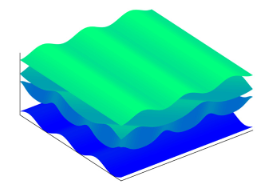
\includegraphics[width=7.6cm]{sections/7_conclusions_and_future_directions/multilayered.png}%
    \vspace{3mm}
    \caption{A five--layer problem configuration with layer interfaces $z = a^{(m)}+g^{(m)}(x).$}%
    \label{fig:example}%
\end{figure}
\vspace{-15mm}
%\begin{flushleft}
A generalization of our analyticity theorems (cf. $\S 4.5$) up to $M$ parameters is included as Theorem~$3.2$ in \cite{Nicholls16b}. For this, we consider quite general systems of linear equations of the form
%\end{flushleft}
\be
\bA(\tEps)\bV(\tEps)=\bR(\tEps),
\ee
where 
\bes
\bA(\tEps)=\sum_{\tn=0}^{\infty}\bA_{\tn}\tEps^{\tn},\quad 
\bR(\tEps) = \sum_{\tn=0}^{\infty}\bR_{\tn}\tEps^{\tn}.
\ees
The tildes represent multi--index notation \cite{Evans10}, in particular
\bes
\tEps := \begin{pmatrix} \Eps_1 \\ \vdots \\ \Eps_M \end{pmatrix},
\quad
\tn := \begin{pmatrix} n_1 \\ \vdots \\ n_M \end{pmatrix},
\ees
and the convention
\bes
\sum_{\tn=0}^{\infty} 
    A_{\tn}\ \tEps^{\tn}
  = \sum_{n_1=0}^{\infty} \cdots \sum_{n_M=0}^{\infty}
    A_{n_1,\ldots,n_M} \Eps_1^{n_1} \cdots \Eps_M^{n_M}.
\ees
As in $\S 4.5$, we seek a solution of the form
\be
\bV(\tEps)=\sum_{\tn=0}^{\infty}\bV_{\tn}\tEps^{\tn},
\ee
and from $(7.1)$ we find at order $\mathcal{O}(\tEps^{\tn})$
\bes
\bA_0\bV_{\tn}= \bR_{\tn} - \left(\sum_{\tl=0}^{\tn}\bA_{\tn-\tl}\bV_{\tl}- \bA_0\bV_{\tn}\right),
\ees
or
\be
\bV_{\tn}= \bA_0^{-1}\left\{\bR_{\tn} - \left(\sum_{\tl=0}^{\tn}\bA_{\tn-\tl}\bV_{\tl}- \bA_0\bV_{\tn}\right)\right\}.
\ee
The above notation represents multi--indices in the form
\bes
\sum_{\tl=0}^{\tn}\bA_{\tn-\tl}\bV_{\tl} = \sum_{\ell_1=0}^{n_1}\cdots \sum_{\ell_M=0}^{n_M}
    \bA_{n_1-\ell_1,\ldots,n_M-\ell_M} \bV_{\ell_1,\ldots,\ell_m},  
\ees
where $\tn=(n_1,\ldots,n_M),$ $\tl=(\ell_1,\ldots,\ell_M),$ and $0=(0,\ldots,0)$ with the convention
\bes
\tn \geq 0 \iff n_1\geq 0,\ldots,n_M\geq 0, \quad\tl \geq 0 \iff \ell_1\geq 0,\ldots,\ell_M\geq 0.
\ees
With these, we can extend our existence theorem (Theorem $4.5.1$) to $M$ parameters.
\begin{theorem}
\label{Thm:AVR}
Given two Banach spaces, $X$ and $Y$, suppose that:
\begin{enumerate}[label={\upshape[\arabic*]}]
\item $\bR_{\tn} \in Y$ for all $\tn \geq 0$,
  and there exist $M$--multi--indexed constants $C_R > 0$, $B_R > 0$,
  \bes
  C_R = \begin{pmatrix} C_{R,1} \\ \vdots \\ C_{R,M} \end{pmatrix},
  \quad
  B_R^{\tn} = \begin{pmatrix} B_{R,1}^{n_1} \\ \vdots \\ 
  B_{R,M}^{n_M} \end{pmatrix},
  \ees
  such that
  \bes
  \Norm{\bR_{\tn}}{Y} \leq C_R B_R^{\tn},
  \ees
\item $\bA_{\tn}: X \rightarrow Y$ for all
  $\tn \geq 0$, and there exist $M$--multi--indexed
  constants $C_A > 0$, $B_A > 0$ such that
  \bes
  \Norm{\bA_{\tn}}{X \rightarrow Y} \leq C_A B_A^{\tn},
  \ees
\item $\bA_0^{-1}: Y \rightarrow X$, and there 
  exists a constant $C_e > 0$ such that
  \bes
  \Norm{\bA_0^{-1}}{Y \rightarrow X} \leq C_e.
  \ees  
\end{enumerate}
Then the equation $(7.1)$ has a unique solution,
\be
\label{Eqn:V:Exp:Multi}
\bV(\tEps) = \sum_{\tn=0}^{\infty} \bV_{\tn} \tEps^{\tn},
\ee
and there exist $M$--multi--indexed constants $C_V > 0$ and $B_V > 0$ such that
\bes
\Norm{\bV_{\tn}}{X} \leq C_V B_V^{\tn},
\ees
for all $\tn \geq 0$ and any
\bes
C_V \geq 2 C_e C_R,
\quad
B_V \geq \max \left\{ B_R, 2 B_A, 2^{M+1} C_e C_A B_A \right\},
\ees
enforced componentwise. This implies that, for any $M$--multi--indexed constant
$0 \leq \tilde{\rho} < 1$, 
$(7.4)$, converges for all $\tEps$ such that
$B \tEps < \tilde{\rho}$, i.e., $\tEps < \tilde{\rho}/B$.
\end{theorem}
\begin{remark}
Our proof strategy is a form of multidimensional induction where given a statement $\bP(n_1, n_2, n_3, ..., n_M)$ for some $M\in \mathbb{N}$, we will show that $\forall n_1, n_2,\ldots, n_M \geq 0$, $\bP(n_1, n_2, n_3, ..., n_M)$ is true by inducting on $n_M$. We will follow the steps outlined below.
\begin{enumerate}
\item Establish $\bP(0,\ldots,n_j,\ldots,0)$ for all $1 \leq j < M$ and $n_1,\ldots,n_j \geq 0.$
\item Given $\bP(n_1,n_2,\ldots,n_j,\ldots,0)$ for all $1 \leq j < M$ and $n_1,\ldots,n_j \geq 0$, establish $\bP(n_1,n_2,\ldots,\bar{n}_j,\ldots,0)$. This can be accomplished through the two steps below.
\begin{enumerate}
    \item Establish $\bP(0,\ldots,\bar{n}_j,\ldots,0)$ for all $\bar{n}_j \geq 0$ (where the hypothesis in $[2]$ gives the required case for $n_j < \bar{n}_j$).
    \item Given  $\bP(n_1,n_2,\ldots,\bar{n}_j,\ldots,0)$ for all $1 \leq j < M$ and $n_1 < \bar{n}_1,  n_2 < \bar{n}_2,\ldots, $ $n_{j-1}  < \bar{n}_{j-1}$ and $\bar{n}_j\geq 0$, establish $\bP(\bar{n}_1,\bar{n}_2,\ldots,\bar{n}_j,\ldots,0)$.
\end{enumerate}
\item Given $\bP(n_1,n_2,\ldots,n_j,n_{j+1},\ldots,0)$ for all $1 \leq j+1 < M$ and $n_1,\ldots,n_{j+1} \geq 0$, establish $\bP(n_1,n_2,\ldots,n_j,\bar{n}_{j+1},\ldots,0)$. This can be accomplished by following the two steps outlined below. 
\begin{enumerate}
    \item Establish $\bP(0,\ldots,\bar{n}_{j+1},\ldots,0)$ for all $\bar{n}_{j+1} \geq 0$ (where the hypothesis in $[3]$ gives the required case for $n_{j+1} < \bar{n}_{j+1}$).
    \item Given  $\bP(n_1,n_2,\ldots,n_j,\bar{n}_{j+1},\ldots,0)$ for all $1 \leq j+1 < M$ and  $n_1 < \bar{n}_1,  n_2 < \bar{n}_2,\ldots, n_{j} < \bar{n}_{j}$ and $\bar{n}_{j+1}\geq 0$, establish $\bP(\bar{n}_1,\bar{n}_2,\ldots,\bar{n}_j,\bar{n}_{j+1}\ldots,0)$.
\end{enumerate}
\item Given $\bP(n_1,n_2,\ldots,n_{M-1},n_M)$ for all $n_1,n_2,\ldots,n_{M-1} \geq 0$ and $n_M < \bar{n}_M$, establish $\bP(n_1,n_2,\ldots,n_{M-1},\bar{n}_M)$. This can be accomplished by the two steps below (the base cases are handled through $[2]$ and $[3]$).
\begin{enumerate}
    \item Establish $\bP(0,\ldots,\bar{n}_{M})$ for $\bar{n}_{M} \geq 0$ (where the hypothesis in $[4]$ handles the required case for  $n_{M} < \bar{n}_{M}$).
    \item Given $\bP(n_1,n_2,\ldots,n_{M-1},\bar{n}_M)$ for all $n_1 < \bar{n}_1, n_2 < \bar{n}_2, \ldots n_{M-1} < \bar{n}_{M-1}$ and $\bar{n}_M \geq 0$, establish $\bP(\bar{n}_1,\bar{n}_2,\ldots,\bar{n}_{M-1},\bar{n}_M)$.
\end{enumerate}
\end{enumerate}

\end{remark}

\begin{proof}{[Theorem 7.4.1]} As with $\tEps$ and $\tn$, we represent $\tilde{\rho}$ by
\bes
\tilde{\rho} := \begin{pmatrix} \rho_1 \\ \vdots \\ \rho_M \end{pmatrix}.
\ees
As before, we will work by induction and consider the general case for finite $M>0$ where we want to establish
\bes
\norm{\bV_{n_1,\ldots,n_M}}_X \leq C_{V,1}\ldots C_{V,M} B_{V,1}^{n_1}\ldots B_{V,M}^{n_M}, \quad \forall n_1,\ldots,n_M\geq 0.
\ees
We prove this via an induction on $n_M$. The base case $n_1,n_2,\ldots, n_{j-1},n_{j+1},\ldots,$ $n_M=0$ and $1 \leq j < M$:
\bes
\norm{\bV_{0,\ldots,n_j,\ldots,0}}_X \leq C_{V,j} B_{V,j}^{n_j}, \quad \forall n_j\geq 0,
\ees
has previously been established by Theorem $4.5.1$ where $\tEps = \Eps_j$ and $\delta=0$. We now assume
\bes
\norm{\bV_{n_1,\ldots,n_j,\ldots,0}}_X \leq  C_{V,1}\ldots C_{V,j}B_{V,1}^{n_1}\ldots B_{V,j}^{n_j}, ~~ \forall n_1,\ldots,n_{j-1}\geq 0,~~ \forall n_j < \bar{n}_j,~~ 1 \leq j < M,
\ees
and seek
\bes
\norm{\bV_{n_1,\ldots,\bar{n}_j,\ldots,0}}_X \leq  C_{V,1}\ldots C_{V,j}B_{V,1}^{n_1}\ldots B_{V,j}^{\bar{n}_j}, ~~ \forall n_1,\ldots,n_{j-1}\geq 0.
\ees
This can be obtained through a chain of $(M-1)$ inductions on $n_1,\ldots,n_j$ where $1 \leq j < M$. For simplicity, we will show what happens in the arbitrary case $n_j$. The base case $n_1,\ldots,n_{j-1}=0$:
\bes
\norm{\bV_{0,\ldots,\bar{n}_j,\ldots,0}}_X \leq  C_{V,j}B_{V,j}^{\bar{n}_j}, \quad \forall \bar{n}_j \geq 0,
\ees
is established by Theorem $4.5.1$ where $\tEps = \Eps_j$ and $\delta=0$. Therefore, we assume
\begin{align*}
\norm{\bV_{n_1,\ldots,\bar{n}_j,\ldots,0}}_X \leq  C_{V,1}\ldots C_{V,j}B_{V,1}^{n_1}\ldots B_{V,j}^{\bar{n}_j},~~\forall n_1  &< \bar{n}_1,\ldots, n_{j-1} < \bar{n}_{j-1},~~ \forall \bar{n}_j \geq 0,\\&~ 1 \leq j < M,
\end{align*}
and seek
\bes
\norm{\bV_{\bar{n}_1,\ldots,\bar{n}_j,\ldots,0}}_X \leq  C_{V,1}\ldots C_{V,j}B_{V,1}^{\bar{n}_1}\ldots B_{V,j}^{\bar{n}_j}.
\ees
Recalling $\tn=(n_1,\ldots,n_j)$ and  $\tl=(\ell_1,\ldots,\ell_j)$, we define
\be
{\sum_{\tl=0}^{\tn}}^{*}\bA_{\tn-\tl}\bV_{\tl} := \sum_{\tl=0}^{\tn}\bA_{\tn-\tl}\bV_{\tl} - \bA_0\bV_{\tn},
\ee
and apply $(7.3),(7.5)$ and the mapping properties of $\bA_{0}^{-1}$ to find
\bes
\norm{\bV_{\bar{n}_1,\ldots,\bar{n}_j,\ldots,0}}_X\leq C_e\left\{\norm{\bR_{\bar{n}_1,\ldots,\bar{n}_j}}_Y + {\sum_{\tl=0}^{\tn}}^{*}\norm{\bA_{\tn-\tl}\bV_{\tl}}_Y\right\}.
\ees
Using the estimates on $\bR_{n_1,\ldots,n_j}$ and $\bA_{n_1,\ldots,n_j}$ (for all $n_1,\ldots,n_j$) and $\bV_{n_1,\ldots,n_j}$ $(n_1 < \bar{n}_1, \ldots, n_j < \bar{n}_j)$ we have
\begin{align*}
\norm{\bV_{\bar{n}_1,\ldots,\bar{n}_j,\ldots,0}}_X &\leq
C_e\Bigg\{C_{R,1}\ldots C_{R,j}B_{R,1}^{\bar{n}_1}\ldots B_{R,j}^{\bar{n}_j} + {\sum_{\tl=0}^{\tn}}^{*}C_{A,1}\ldots C_{A,j}B_{A,1}^{\bar{n}_1-\ell_1}\ldots B_{A,j}^{\bar{n}_j-\ell_j}\\ & \qquad \qquad \qquad \qquad \qquad \qquad \qquad \qquad \times
C_{V,1}\ldots C_{V,j}B_{V,1}^{\ell_1}\ldots B_{V,j}^{\ell_j}\Bigg\} \\& =
C_eC_{R,1}\ldots C_{R,j}B_{R,1}^{\bar{n}_1}\ldots B_{R,j}^{\bar{n}_j} + C_eC_{A,1}\ldots C_{A,j}C_{V,1}\ldots C_{V,j} \\&
~~ \times \left(\frac{B_{A,1}}{B_{V,1}}\right)B_{V,1}^{\bar{n}_1}\cdots \left(\frac{B_{A,j}}{B_{V,j}}\right)B_{V,j}^{\bar{n}_j}{\sum_{\tl=0}^{\tn}}^{*}
\left(\frac{B_{A,1}}{B_{V,1}}\right)B_{V,1}^{\bar{n}_1-\ell_1-1}\cdots \\& ~~ \times
\left(\frac{B_{A,j}}{B_{V,j}}\right)B_{V,j}^{\bar{n}_j-\ell_j-1} \\& \leq
C_eC_{R,1}\ldots C_{R,j}B_{V,1}^{\bar{n}_1}\ldots B_{V,j}^{\bar{n}_j} + C_eC_{A,1}\ldots C_{A,j}C_{V,1}\ldots C_{V,j} \\& ~~ \times
\left(\frac{B_{A,1}}{B_{V,1}}\right)B_{V,1}^{\bar{n}_1}\cdots\left(\frac{B_{A,j}}{B_{V,j}}\right)B_{V,j}^{\bar{n}_j}\left(\frac{1}{1-1/2}\right)^j,
\end{align*}
if $B_{A,k}/B_{V,k} \leq 1/2$, $k=1,\ldots,j$ (implying $B_{V,k} \geq 2B_{A,k}$). We are done if we demand that
\bes
B_{V,k} \geq B_{R,k}, \quad C_eC_{R,k} \leq C_{V,k}/2, \quad 2^jC_eC_{A,k}C_{V,k}(B_{A,k}/B_{V,k}) \leq 
C_{V,k}/2.
\ees
This can be realized if
\bes
C_{V,k} \geq 2C_eC_{R,k}, \quad
B_{V,k} \geq \max\left\{B_{R,k},2B_{A,k},2^{j+1}C_eC_{A,k}B_{A,k}\right\}.
\ees
We then assume
\begin{align*}
\norm{\bV_{n_1,\ldots,n_{j+1},\ldots,0}}_X \leq  C_{V,1}\ldots C_{V,j+1}B_{V,1}^{n_1}\ldots B_{V,j+1}^{n_{j+1}}, ~~ &\forall n_1,\ldots,n_j\geq 0,~~ \forall n_{j+1} < \bar{n}_{j+1},\\&~~ 1 \leq j < M,
\end{align*}
and seek
\bes
\norm{\bV_{n_1,\ldots,\bar{n}_{j+1},\ldots,0}}_X \leq  C_{V,1}\ldots C_{V,j+1}B_{V,1}^{n_1}\ldots B_{V,j+1}^{\bar{n}_{j+1}}, ~~ \forall n_1,\ldots,n_{j}\geq 0.
\ees
As before, this can be obtained through a chain of $M$ inductions on $n_1,\ldots,n_{j+1}$ where $1 \leq j < M$. For simplicity, we will show what happens in the arbitrary case $n_{j+1}$. The base case $n_1,\ldots,n_{j}=0$:
\bes
\norm{\bV_{0,\ldots,\bar{n}_{j+1},\ldots,0}}_X \leq  C_{V,j+1}B_{V,j+1}^{\bar{n}_{j+1}}, \quad \forall \bar{n}_{j+1} \geq 0,
\ees
is established by Theorem $4.5.1$ where $\tEps = \Eps_{j+1}$ and $\delta=0$. Therefore, we assume
\begin{align*}
\norm{\bV_{n_1,\ldots,\bar{n}_{j+1},\ldots,0}}_X \leq  C_{V,1}\ldots C_{V,j+1}B_{V,1}^{n_1}\ldots B_{V,j+1}^{\bar{n}_{j+1}},~~\forall n_1  &< \bar{n}_1,\ldots, n_{j} < \bar{n}_{j},~~ \forall \bar{n}_{j+1} \geq 0,\\&~ 1 \leq j < M,
\end{align*}
and seek
\bes
\norm{\bV_{\bar{n}_1,\ldots,\bar{n}_{j+1},\ldots,0}}_X \leq  C_{V,1}\ldots C_{V,j+1}B_{V,1}^{\bar{n}_1}\ldots B_{V,j+1}^{\bar{n}_{j+1}}.
\ees
In this scenario, $\tn=(n_1,\ldots,n_{j+1})$ and  $\tl=(\ell_1,\ldots,\ell_{j+1}),$ so we apply $(7.3),(7.5)$ and the mapping properties of $\bA_{0}^{-1}$ to find
\bes
\norm{\bV_{\bar{n}_1,\ldots,\bar{n}_{j+1},\ldots,0}}_X\leq C_e\left\{\norm{\bR_{\bar{n}_1,\ldots,\bar{n}_{j+1}}}_Y + {\sum_{\tl=0}^{\tn}}^{*}\norm{\bA_{\tn-\tl}\bV_{\tl}}_Y\right\}.
\ees
Using the estimates on $\bR_{n_1,\ldots,n_{j+1}}$ and $\bA_{n_1,\ldots,n_{j+1}}$ (for all $n_1,\ldots,n_{j+1}$) and $\bV_{n_1,\ldots,n_{j+1}}$ $(n_1 < \bar{n}_1, \ldots, n_{j+1} < \bar{n}_{j+1})$ we have
\begin{align*}
\norm{\bV_{\bar{n}_1,\ldots,\bar{n}_{j+1},\ldots,0}}_X &\leq
C_e\Bigg\{C_{R,1}\ldots C_{R,{j+1}}B_{R,1}^{\bar{n}_1}\ldots B_{R,{j+1}}^{\bar{n}_{j+1}} + {\sum_{\tl=0}^{\tn}}^{*}C_{A,1}\ldots C_{A,{j+1}}B_{A,1}^{\bar{n}_1-\ell_1}\ldots \\ & \qquad \qquad \qquad \qquad \qquad \quad \times
B_{A,{j+1}}^{\bar{n}_{j+1}-\ell_{j+1}}C_{V,1}\ldots C_{V,{j+1}}B_{V,1}^{\ell_1}\ldots B_{V,{j+1}}^{\ell_{j+1}}\Bigg\} \\& =
C_eC_{R,1}\ldots C_{R,{j+1}}B_{R,1}^{\bar{n}_1}\ldots B_{R,{j+1}}^{\bar{n}_{j+1}} + C_eC_{A,1}\ldots C_{A,{j+1}}C_{V,1}\ldots C_{V,{j+1}} \\&
~~ \times \left(\frac{B_{A,1}}{B_{V,1}}\right)B_{V,1}^{\bar{n}_1}\cdots \left(\frac{B_{A,{j+1}}}{B_{V,{j+1}}}\right)B_{V,{j+1}}^{\bar{n}_{j+1}}{\sum_{\tl=0}^{\tn}}^{*}
\left(\frac{B_{A,1}}{B_{V,1}}\right)B_{V,1}^{\bar{n}_1-\ell_1-1}\cdots \\& ~~ \times
\left(\frac{B_{A,{j+1}}}{B_{V,{j+1}}}\right)B_{V,{j+1}}^{\bar{n}_{j+1}-\ell_{j+1}-1} \allowdisplaybreaks\\& \leq
C_eC_{R,1}\ldots C_{R,{j+1}}B_{V,1}^{\bar{n}_1}\ldots B_{V,{j+1}}^{\bar{n}_{j+1}} + C_eC_{A,1}\ldots C_{A,{j+1}}C_{V,1}\ldots C_{V,{j+1}} \\& ~~ \times
\left(\frac{B_{A,1}}{B_{V,1}}\right)B_{V,1}^{\bar{n}_1}\cdots\left(\frac{B_{A,{j+1}}}{B_{V,{j+1}}}\right)B_{V,{j+1}}^{\bar{n}_{j+1}}\left(\frac{1}{1-1/2}\right)^{j+1},
\end{align*}
if $B_{A,t}/B_{V,t} \leq 1/2$, $t=1,\ldots,j+1$ (implying $B_{V,t} \geq 2B_{A,t}$). We are done if we demand that
\bes
B_{V,t} \geq B_{R,t}, \quad C_eC_{R,t} \leq C_{V,t}/2, \quad 2^{j+1}C_eC_{A,t}C_{V,t}(B_{A,t}/B_{V,t}) \leq 
C_{V,t}/2.
\ees
This can be realized if
\bes
C_{V,t} \geq 2C_eC_{R,t}, \quad
B_{V,t} \geq \max\left\{B_{R,t},2B_{A,t},2^{j+2}C_eC_{A,t}B_{A,t}\right\}.
\ees
To complete the general case for finite $M>0$, we assume
\bes
\norm{\bV_{n_1,\ldots,n_M}}_X \leq  C_{V,1}\ldots C_{V,M}B_{V,1}^{n_1}\ldots B_{V,M}^{n_M}, ~~ \forall n_1,\ldots,n_{M-1}\geq 0,~~ \forall n_M < \bar{n}_M,
\ees
and seek
\bes
\norm{\bV_{n_1,\ldots,\bar{n}_M}}_X \leq  C_{V,1}\ldots C_{V,M}B_{V,1}^{n_1}\ldots B_{V,M}^{\bar{n}_M}, ~~ \forall n_1,\ldots,n_{M-1}\geq 0.
\ees
The base case $n_1,n_2,\ldots,n_{M-1}=0$:
\bes
\norm{\bV_{0,\ldots,\bar{n}_M}}_X \leq  C_{V,M}B_{V,M}^{\bar{n}_M}, \quad \forall \bar{n}_M \geq 0,
\ees
has previously been established by Theorem $4.5.1$ where $\tEps = \Eps_M$ and $\delta =0$. Finally, we assume
\begin{align*}
\norm{\bV_{n_1,\ldots,n_{M-1},\bar{n}_M}}_X \leq  C_{V,1}\ldots C_{V,M}B_{V,1}^{n_1}\ldots B_{V,M}^{\bar{n}_M},~~~&\forall n_1  < \bar{n}_1,\ldots, n_{M-1} < \bar{n}_{M-1},\\&~~~~ \forall \bar{n}_M \geq 0,
\end{align*}
and seek
\bes
\norm{\bV_{\bar{n}_1,\ldots,\bar{n}_{M-1},\bar{n}_M}}_X \leq  C_{V,1}\ldots C_{V,M}B_{V,1}^{\bar{n}_1}\ldots B_{V,M}^{\bar{n}_M}.
\ees
In this case, $\tn=(n_1,\ldots,n_M)$ and  $\tl=(\ell_1,\ldots,\ell_M),$ so we apply $(7.3),(7.5)$ and the mapping properties of $\bA_{0}^{-1}$ to find
\bes
\norm{\bV_{\bar{n}_1,\ldots,\bar{n}_M}}_X\leq C_e\left\{\norm{\bR_{\bar{n}_1,\ldots,\bar{n}_M}}_Y + {\sum_{\tl=0}^{\tn}}^{*}\norm{\bA_{\tn-\tl}\bV_{\tl}}_Y\right\}.
\ees
Using the estimates on $\bR_{n_1,\ldots,n_M}$ and $\bA_{n_1,\ldots,n_M}$ (for all $n_1,\ldots,n_M$) and $\bV_{n_1,\ldots,n_M}$ $(n_1 < \bar{n}_1, \ldots, n_M < \bar{n}_M)$ we have
\vspace{-1.5mm}
\begin{align*}
\norm{\bV_{\bar{n}_1,\ldots,\bar{n}_M}}_X &\leq
C_e\Bigg\{C_{R,1}\ldots C_{R,M}B_{R,1}^{\bar{n}_1}\ldots B_{R,M}^{\bar{n}_M} + {\sum_{\tl=0}^{\tn}}^{*}C_{A,1}\ldots C_{A,M}B_{A,1}^{\bar{n}_1-\ell_1}\ldots B_{A,M}^{\bar{n}_M-\ell_M}\\ & \qquad \qquad \qquad \qquad \qquad \qquad \qquad \qquad \times
C_{V,1}\ldots C_{V,M}B_{V,1}^{\ell_1}\ldots B_{V,M}^{\ell_M}\Bigg\} \\& =
C_eC_{R,1}\ldots C_{R,M}B_{R,1}^{\bar{n}_1}\ldots B_{R,M}^{\bar{n}_M} + C_eC_{A,1}\ldots C_{A,M}C_{V,1}\ldots C_{V,M} \\& 
~~ \times \left(\frac{B_{A,1}}{B_{V,1}}\right)B_{V,1}^{\bar{n}_1}\cdots \left(\frac{B_{A,M}}{B_{V,M}}\right)B_{V,M}^{\bar{n}_M}{\sum_{\tl=0}^{\tn}}^{*}
\left(\frac{B_{A,1}}{B_{V,1}}\right)B_{V,1}^{\bar{n}_1-\ell_1-1}\cdots \\& \allowdisplaybreaks~~ \times
\left(\frac{B_{A,M}}{B_{V,M}}\right)B_{V,M}^{\bar{n}_M-\ell_M-1} \\&  \leq
C_eC_{R,1}\ldots C_{R,M}B_{V,1}^{\bar{n}_1}\ldots B_{V,M}^{\bar{n}_M} + C_eC_{A,1}\ldots C_{A,M}C_{V,1}\ldots C_{V,M} \\& ~~ \times
\left(\frac{B_{A,1}}{B_{V,1}}\right)B_{V,1}^{\bar{n}_1}\cdots\left(\frac{B_{A,M}}{B_{V,M}}\right)B_{V,M}^{\bar{n}_M}\left(\frac{1}{1-1/2}\right)^M,
\end{align*}
if $B_{A,i}/B_{V,i} \leq 1/2$, $i=1,\ldots,M$ (implying $B_{V,i} \geq 2B_{A,i}$). We are done if we demand that
\bes
B_{V,i} \geq B_{R,i}, \quad C_eC_{R,i} \leq C_{V,i}/2, \quad 2^MC_eC_{A,i}C_{V,i}(B_{A,i}/B_{V,i}) \leq 
C_{V,i}/2.
\ees
This can be realized if
\bes
C_{V,i} \geq 2C_eC_{R,i}, \quad
B_{V,i} \geq \max\left\{B_{R,i},2B_{A,i},2^{M+1}C_eC_{A,i}B_{A,i}\right\}.
\ees
\end{proof}
Using a similar approach in conjunction with the analysis in Chapters $2$ and $3$, we predict a more general form of Theorems $2.9.2$ and $3.8.1$ exists, which would establish the analyticity of the transformed field with respect to any finite $M > 0$ perturbation parameters.
\vspace{1mm}
\begin{conjecture} 
\label{Conj:u,w:Anal:n:n_m}
Given any integer $s \geq 0$, if $f \in C^{s+2}([0,d])$ and 
$U_{\tilde{n}} \in H^{s+3/2}([0,d])$, $W_{\tilde{n}}\in H^{s+3/2}([0,d])$ such that
\bes
\|U_{\tilde{n}}\|_{H^{s+3/2}} \le K_U B_U^{\tn} , \quad
\|W_{\tilde{n}}\|_{H^{s+3/2}} \le K_W B_W^{\tn} ,
\ees
for constants $K_U, K_W>0$ and $M$--multi--indexed constants $B_U, B_W > 0$, then 
$u_{\tn} \in H^{s+2}([0,d]\times[0,a])$, $w_{\tn}\in H^{s+2}([0,d]\times[-b,0])$ and
\bes
\label{Eqn:u,w:Est:n:n_m}
\|u_{\tn}\|_{H^{s+2}} \le K B^{\tn}, \quad
\|w_{\tn}\|_{H^{s+2}} \le \tilde{K}\tilde{B}^{\tn} ,
\ees
for constants $K,\tilde{K}> 0$ and $M$--multi--indexed constants $B ,\tilde{B}>0$.
\end{conjecture}
\vspace{1mm}
Analogously, a similar procedure would establish a more general form of Theorems $2.10.2$ and $3.9.2$ for the analyticity of the DNOs for any finite $M>0$ perturbation parameters.
\vspace{1mm}
\begin{conjecture} 
\label{Thm:G,J:Anal:n:n_m}
Given any integer $s \geq 0$, if $f \in C^{s+2}([0,d])$ and 
$U_{\tn} \in H^{s+3/2}([0,d])$, $W_{\tn} \in H^{s+3/2}([0,d])$ such that
\bes
\SobNorm{U_{\tn}}{s+3/2} \leq K_U B_U^{\tn}, \quad
\SobNorm{W_{\tn}}{s+3/2} \leq K_W B_W^{\tn},
\ees
for constants $K_U,K_W> 0$ and $M$--multi--indexed constants $B_U, B_W > 0$, then $G_{\tn} \in H^{s+1/2}([0,d])$, $J_{\tn} \in H^{s+1/2}([0,d])$ and
\bes
\label{Eqn:G,J:Est:n:n_m} 
\|G_{\tn}\|_{H^{s+1/2}} \le \tilde{K}\tilde{B}^{\tn}, \quad
\|J_{\tn}\|_{H^{s+1/2}} \le \dbtilde{K} \dbtilde{B}^{\tn},
\ees
for constants $\tilde{K},\dbtilde{K}  > 0$ and $M$--multi--indexed constants $\tilde{B},\dbtilde{B}>0$.
\end{conjecture}
\vspace{1mm}
Upon proving these, one has two key ingredients to the more general version of Theorem $4.6.1$ which establishes the existence and uniqueness of solutions to a system of partial differential equations with respect to $M$ perturbation parameters.
\vspace{1mm}
\begin{conjecture} 
\label{Conj:Main}
Given an integer $s \geq 0$, if $f \in C^{s+2}([0,d])$ then the 
equation $(7.1)$ has a unique solution, $(7.4)$,
and there exist a constant $C > 0$ and $M$--multi--indexed constants $B>0$ such that
\bes
\Norm{\bV_{\tn}}{X^s} \leq C B^{\tn},
\ees
for all $\tn \geq 0$.  This implies that for any $M$--multi--indexed constant
$0 \leq \tilde{\rho} < 1$, $(7.4)$, converges for all $\tEps$ such that
$B \tEps < \tilde{\rho}$, i.e., $\tEps < \tilde{\rho}/B$.
\end{conjecture}
\vspace{1mm}
\textbf{Predictions:} In application oriented fields such as signal processing or sea ice modeling, practitioners work with  multiple frequencies \cite{qiu2005high,bosse1995model,zhao2009multi,blanchard2021high} at short or long wavelengths. Also, as depicted in Figure $35$, the grating surface could have $M$ different layers \cite{imperatore2017perturbation} with distinct values of $g_j(x)=\Eps f_j(x),~j=1,\ldots, M$. A proof of Conjecture $7.4.4$ would enable the freedom to enforce any number of perturbation parameters and obtain an analytic solution. Given the widespread availability of parallel computing resources coupled with additional perturbation parameters associated with elastic media, we believe that future research will force hundreds or even thousands of distinct perturbation parameters, all of which should yield an analytic solution.
\section{Parallel Programming}
\setcounter{section}{5}
\label{Sec: Parallel Programming}

In the case of multiple layered interfaces, we need to compute intermediate DNOs for up to $M$ layers. This will greatly increase the computational cost and execution time of our HOPS/AWE algorithm and we suspect that it will be necessary to introduce parallel programming techniques to offset the computational expense. In the context of the \gls{oe} method, preliminary work \cite{fang2015operator} has been completed in C\texttt{++} to parallelize the computation of Navier's equations \cite{BillinghamKing00,achenbach2012wave}. These techniques can be adapted to the TFE method through the choice of OpenMP \cite{chandra2001parallel}, MPI \cite{snir1998mpi}, or CUDA \cite{sanders2010cuda}.
\newline
\\
\textbf{Predictions:} In two or three dimensions, our HOPS code is robust, efficient and has a runtime less than an hour. A local machine with an Intel Core i$5$ CPU, $8$GB of RAM, and Windows $10$ OS completed almost every simulation in this thesis in less than thirty minutes. However, with ten to one hundred layer configurations, we suspect that many simulations will take on the order of weeks or even months. As a result, it will be necessary to parallelize our Matlab code in a compiled programming language such as C or  C\texttt{++}.

\section{Alternatives to DNOs}
\label{Sec: Alternatives to DNOs}
In Chapter $4$ we wrote our scattering problem as a linear system
\bes
\bA \bV = \bR,
\ees
where, upon expanding $\{\bA,\bV,\bR\}$ in both $\varepsilon$ and $\delta$, we arrived at the flat--interface solution $\bA_{0,0}\bV_{0,0}=\bR_{0,0}$
at order $\mathcal{O}(\varepsilon^0,\delta^0)$. We then saw it was necessary to invert
\bes
\bA_{0,0} = \begin{pmatrix}I & -I\\
-G_{0,0} & -\tau^2J_{0,0}\end{pmatrix}, 
\ees
which features the two DNOs, $G_{0,0}$ and $J_{0,0}$, in order to show the existence and uniqueness of solutions. A primary feature of all HOPS schemes is the inversion of a single, sparse operator $\bA_{0,0}$ through the use of DNOs. However, one may ponder if a different technique could produce a more competitive algorithm that is comparable to our HOPS/AWE algorithm (or even better). Is it absolutely necessary to pass in transformed field data in order to efficiently compute and recover internal information stored at the grating surface?
\\
\newline
\textbf{Predictions:} A primary advantage of our HOPS/AWE scheme is that for every perturbation order, it is only necessary to invert a single sparse operator corresponding to a flat--interface, order--zero approximation. There are a number of competing approaches in general perturbation theory within the context of layered media problems. In regards to electromagnetic wave scattering, Galerkin and boundary element methods are discussed in \cite{escapil2020helmholtz,silva2017quantifying,nakata1990boundary,elschner2012optimization,rathsfeld2006} and a high--order perturbation approach based on boundary integral equations in \cite{dolz2020higher}. High--order schemes for linear waves can be computed using level set methods \cite{sethian1999level} and fast marching methods, as well as other methods involving domain decomposition \cite{el2004comparing,benamou1997domain,larsson1999domain,gong2021convergence,perez2018domain,chan1994domain}. A holistic evaluation of these competing methods could potentially improve our HOPS/AWE algorithm if we found a faster method of inverting linear operators without the use of DNOs.
\section{Computational Complexity}
\label{Sec: Computational Complexity}

One of the fundamental reasons for developing our HOPS/AWE algorithm is its advantageous computational complexity for problems within its domain of applicability.
In comparison with other classical methods, our HOPS/AWE approach has several advantages for computing quantities such as the Reflectivity Map, $R=R(\varepsilon,\delta)$. To demonstrate this we begin
by fixing the problem of computing $R$ for $N_{\Eps}$ many values of 
$\Eps$ and $N_{\delta}$ many values of $\delta$.

In the case of computing the DNOs $G$ and $J$, we recall from $\S 2.11$ and $\S 3.10$ that our HOPS/AWE algorithm requires
$N_x \times N_z$ unknowns at every perturbation order, $(n,m)$, corresponding to
the $N_x$ equally--spaced gridpoints in the lateral direction and the $N_z + 1$ collocation points in the vertical dimension. In $\S 4.5$ we saw that we could write our scattering problem as $\bA(\Eps,\delta) \bV(\Eps,\delta) = \bR(\Eps,\delta)$ where
\bes
    \bA(\Eps,\delta)=\sumn \summ \bA_{n,m}\Eps^n\delta^m, \quad \bR(\Eps,\delta) = \sumn \summ \bR_{n,m}\Eps^{n}\delta^m,
\ees
and
\bes
\label{Eqn:Soln:Two_Param_Append}
\bV(\Eps,\delta) = \sumn \summ \bV_{n,m}\Eps^{n}\delta^m.
\ees
At order $\mathcal{O}(\Eps^n,\delta^m)$ this becomes
\begin{align}
\begin{split}
\bA_{0,0}\bV_{n,m}=&~\bR_{n,m}-\sum_{\ell=0}^{n-1}\bA_{n-\ell,0}\bV_{\ell,m}-\sum_{r=0}^{m-1}\bA_{0,m-r}\bV_{n,r}\\&
-\sum_{\ell=0}^{n-1}\sum_{r=0}^{m-1}\bA_{n-\ell,m-r}\bV_{\ell,r}.
\end{split}
\end{align}
A careful study of $(7.6)$
reveals that the computational complexity of forming the
right--hand side at order $(n,m)$ is
\bes
\BigOh{n m N_x \log(N_x) N_z \log(N_z)}.
\ees
Inverting the operator $\bA_{0,0}$ has complexity $\BigOh{N_x \log(N_x) N_z \log(N_z)}$
so the full cost of computing the $\bV_{n,m}$, 
$\{ 0 \leq n \leq N, 0 \leq m \leq M \}$, is
\bes
\BigOh{N^2 M^2 N_x \log(N_x) N_z \log(N_z)}.
\ees
Once these coefficients are recovered, the cost of summing the series in 
$(\Eps,\delta)$ is minimal, provided it is done in an efficient manner 
(e.g., by Horner's rule \cite{BurdenFaires,AtkinsonHan01}). Our algorithm then 
requires an additional $\BigOh{N_{\Eps} N_{\delta}}$ steps to sum 
over every value of $(\Eps,\delta)$, therefore the full cost of 
computing the Reflectivity Map by our HOPS/AWE method is
\be
\BigOh{N^2 M^2 N_x \log(N_x) N_z \log(N_z) + N_{\Eps} N_{\delta}}.
\ee
In contrast, for a single $(\Eps,\delta)$ pair, a Boundary Integral Method solver with $N_x$ lateral
gridpoints requires time proportional to $\BigOh{N_x^3}$ for Gaussian elimination
to solve the resulting dense system of $N_x$ equations in $N_x$ unknowns
\cite{BurdenFaires,AtkinsonHan01,ColtonKress13}. Applying this 
$N_{\Eps} \times N_{\delta}$ times results in a total computational complexity of
\be
\BigOh{N_x^3 N_{\Eps} N_{\delta}}.
\ee
Thus, once $N_{\Eps}$ and $N_{\delta}$ become large, e.g.,

\bes
N_{\Eps} N_{\delta} > \frac{N^2 M^2 N_x \log(N_x) N_z \log(N_z)}{N_x^3},
\ees
our new algorithm becomes far more efficient. We speculate that the cost of $(7.7)$ could be reduced to
\be
\BigOh{N M \log(NM)N_x \log(N_x) N_z \log(N_z) + N_{\Eps} N_{\delta}},
\ee
provided that we develop a more efficient method of computing the $\bV_{n,m}$, 
$\{ 0 \leq n \leq N, 0 \leq m \leq M \}$, such as reducing the problem space at every step. Alternative approaches to layered media problems have also been proposed by other authors \cite{bai2004reduction,chew2005fast}, including interpolation \cite{atkins2010fast} and Green's function \cite{konno2016fast}.
\newline
\\
\textbf{Predictions:} The combination of implementing parallel programming techniques (through, e.g., OpenMP or CUDA) and reducing the problem space at every step will greatly enhance the speed and fidelity of our HOPS/AWE algorithm. Considering the natural advantage surface methods have over conventional methods, such as finite difference, finite element, and spectral element methods, we expect that our HOPS/AWE algorithm will be among the most competitive available for periodic layered media problems.
\chapter{Conclusions and Future Work}
\label{sec:conclusions_and_future_dir}

\fancyhead[LO]{\text{Chapter 7}\quad \text{Conclusions and Future Work}}

This thesis establishes a novel HOPS/AWE algorithm that is particularly well suited to simulating scattering returns for periodic media problems. Our main contribution is that of Theorem $4.6.1$ which guarantees the existence and uniqueness of solutions to a system of partial differential equations which model the interaction of linear waves in periodic layered structures with respect to multiple perturbation parameters. Through the introduction of DNOs and a change of variables based on the TFE methodology, we have shown that solutions to the Helmholtz problem are jointly analytic with respect to both interfacial and frequency perturbations. As a result, our HOPS/AWE algorithm is able to handle a variety of numerical simulations that are physically challenging in both the TE and TM polarization modes. Moreover, our extensive numerical results demonstrate the accuracy, speed, and robustness expected of all HOPS methods.


\section{Future Directions}
\label{Sec: Future Directions}
There are a wide range of improvements to both the HOPS/AWE algorithm and the proof of analyticity for linear waves in periodic layered media. Our main goals for future research are to expand the TFE method through a new proof of convergence, investigate expanding around singularities, evaluate analyticity theorems in multilayered configurations, add new parallel programming functionality, explore alternative methods to recover surface data without Dirichlet--Neumann Operators, and to reduce the execution time of the HOPS algorithm. We now summarize these six research goals and suggest predictions for future research.
\begin{enumerate}[labelsep=0ex,align=left,start=1]
    \item[\textbf{Goal 1-}] ~\textbf{Choice of Parameters: Does the geometry of the perturbation impact how large the size of the perturbation can be? }
    \item[\textbf{Goal 2-}] ~\textbf{Rayleigh Singularities: Can we build a full HOPS algorithm based on points where the Taylor expansion is invalid? }
    \item[\textbf{Goal 3-}] ~\textbf{Multiple Layers: Can we prove analyticity results when the number of layers is greater than three? Do the same theorems hold for ten or one hundred layers?} 
    \item[\textbf{Goal 4-}] ~\textbf{{Parallel Programming}: Can we implement parallel programming techniques so that our HOPS code runs on $N$ processors? }
    \item[\textbf{Goal 5-}] ~\textbf{{Alternatives to DNOs}: Do we need to use DNOs to recover surface data from information stored in the transformed field? Is there an alternative method which preserves the inversion of a single, sparse operator at the interface?   }
    \item[\textbf{Goal 6-}] ~\textbf{Computational Costs: Can we reduce the execution time per time step in our HOPS algorithm?} 
\end{enumerate}

\section{Choice of Parameters}
\label{Sec: Choice of Parameters}
Our HOPS/AWE algorithm is based on two smallness assumptions:
\begin{enumerate}
\item \text{Boundary Perturbation: $g(x)=\varepsilon f(x),$ $\varepsilon\in\mathbb R$, $\varepsilon \ll 1$,}
\vspace{-2mm}
\item \text{Frequency Perturbation: $\omega=(1+\delta)\underline{\omega}=\underline{\omega}+\delta\underline{\omega},$ $\omega\in\mathbb R$, $\delta \ll 1$,} 
\end{enumerate}
with the additional assumption that $f$ is sufficiently smooth ($f\in C^2$ \cite{NichollsReitich99,NichollsReitich03b} or even Lipschitz \cite{hu2005analyticity}). Numerical simulations show that our HOPS/AWE algorithm can handle larger perturbations of $\varepsilon$ (the height/slope) in comparison to $\delta$ (the frequency). With modest test parameters and a period of $d=2\pi$, we are able to perturb the value of $\varepsilon$ (to $\varepsilon=0.1$ or even $\varepsilon=0.2$) and still get reasonable convergence results. At a value around $\varepsilon = 10^{-4}$, our HOPS/AWE algorithm converges to machine precision provided that we sum to high enough Taylor orders.
\vspace{-13mm}
\begin{figure}[H]
    \centering
    \subfloat[\centering Large $\varepsilon$, Small $\delta$ ]{{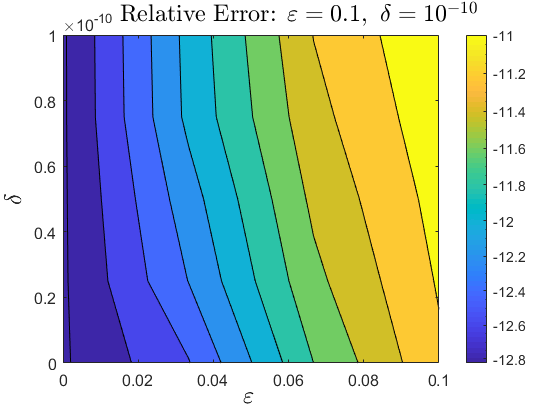
\includegraphics[width=7.6cm]{sections/7_conclusions_and_future_directions/Large_Eps_Small_Delta_2.png} }}%
    %\qquad
    \subfloat[\centering Small $\varepsilon$, Large $\delta$ ]{{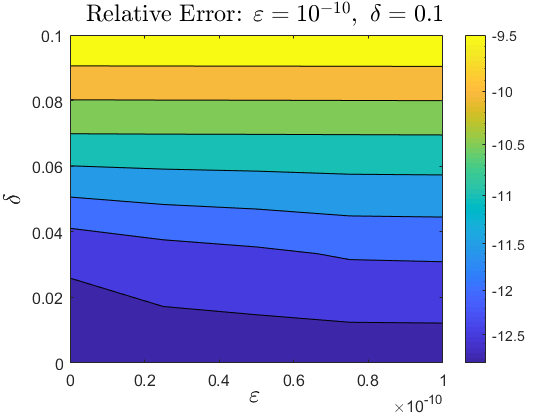
\includegraphics[width=7.6cm]{sections/7_conclusions_and_future_directions/Small_Eps_Large_Delta_2.png} }}%
    \vspace{3 mm}
    \caption{A contour plot of the relative error computed with our HOPS/AWE algorithm by holding $N=M=8$ Taylor orders fixed. In Figure $34\text{(a)}$ we expand up to $\Eps = 0.1$ and $\delta = 10^{-10}$ simultaneously with $N=M=8$ Taylor orders. In Figure $34\text{(b)}$ we expand up to $\Eps = 10^{-10}$ and $\delta = 0.1$ simultaneously with $N=M=8$ Taylor orders.}%
    \label{fig:example}%
\end{figure}
\vspace{-18mm}
Supplementary testing in both the upper and lower layers confirms that our HOPS/AWE algorithm is better suited towards larger $\varepsilon$.
%\begin{flushleft}
\newline
\\
\textbf{Predictions:} Our HOPS/AWE methodology takes advantage of exact enforcement of the \gls{owc} at an artificial boundary in order to truncate the computational domain to one of finite extent. After flattening the surface, the DNOs recover information through the solution stored at the interface. We suspect that this process mitigates large perturbations of the height/slope. By following techniques developed in \cite{NichollsReitich00b,NichollsTaber06,Nicholls16b,NichollsShen08}, we intend to rigorously prove that the TFE method is analytic when $\varepsilon$ is large. Additionally, we are interested in perturbing other physical parameters in the context of layered media problems. These are discussed in the engineering literature \cite{mashayekh2018parameter,mashayekh2018parameter2}.
\section{Rayleigh Singularities}
\label{Sec: Rayleigh Singularities}
A fundamental equation in the HOPS/AWE algorithm is
$$\alpha_p^2 + (\gamma_p^q(\delta))^2 = (k^q)^2,$$
where $k^q$ represents the wavenumber, $q\in\{u,w\}$, and $\alpha=k^q\sin(\theta), \gamma=k^q\cos(\theta),$ are parameters corresponding to refraction/reflection of the incidence angle $\theta$. As shown in $\S 5.4$, a Rayleigh singularity (or Wood's anomaly) occurs when $\ualpha_p^2 = (\uk^q)^2$ for any integer $p\neq 0$. That is, if $\ugamma_p^q(\delta) =0$ for $p\neq 0$ then the Taylor series expansion of $\gamma_p^q(\delta)$ is invalid. In \cite{Nicholls16}, the author investigated changing the Taylor expansion to a Puiseux expansion \cite{basu2007algorithms}:
$$\gamma_p^q(\delta)=\sum_{m=0}^{\infty}\gamma_{p,m}^q\delta^{m+1/2}=\delta^{1/2}\sum_{m=0}^{\infty}\gamma_{p,m}^q\delta^m.$$
However, he found that this approach ran into external difficulties ($\S$6 of \cite{Nicholls16}) simplifying explicit forms of the Dirichlet and Neumann trace operators.
\newline
\\
\textbf{Predictions:} Rayleigh singularities are a central obstruction to the convergence of our HOPS/AWE algorithm. In all of our numerical tests, we select custom frequency ranges which maximize the radius of convergence of our algorithm by expanding away from the singularities (cf. $\S 5.6$). Alternative methods such as Padé summation also fail to be analytic in a neighborhood of a Rayleigh singularity. General perturbation theory provides a variety of known techniques \cite{suslov2005divergent,convfromdiv,Heinz2020,dienes1957taylor,arteca1984summation} for expanding around divergent perturbation series. We suspect that adding these techniques to our HOPS/AWE algorithm will allow us perform a series expansion of $\ugamma_p^q(\delta)$ that does not diverge when $\ugamma_p^q(\delta)=0.$
\section{Multiple Layers}
\label{Sec: Multiple Layers}

In \cite{Nicholls16b}, the author discusses how to apply our HOPS methodology in multilayered configurations. He considers a multilayered material with $M$ (finite) interfaces at 
$$z=a^{(m)}+g^{(m)}(x,y),\quad 1\leq m \leq M,$$
which are $d_x \times d_y$ periodic
$$g^{(m)}(x+d_x,y+d_y)=g^{(m)}(x,y),\quad 1\leq m \leq M,$$
separating $(M+1)$--many layers.
%\vspace{-12mm}
\begin{figure}[H]
    \centering
    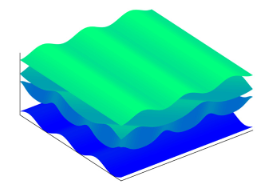
\includegraphics[width=7.6cm]{sections/7_conclusions_and_future_directions/multilayered.png}%
    \vspace{3mm}
    \caption{A five--layer problem configuration with layer interfaces $z = a^{(m)}+g^{(m)}(x).$}%
    \label{fig:example}%
\end{figure}
\vspace{-15mm}
%\begin{flushleft}
A generalization of our analyticity theorems (cf. $\S 4.5$) up to $M$ parameters is included as Theorem~$3.2$ in \cite{Nicholls16b}. For this, we consider quite general systems of linear equations of the form
%\end{flushleft}
\be
\bA(\tEps)\bV(\tEps)=\bR(\tEps),
\ee
where 
\bes
\bA(\tEps)=\sum_{\tn=0}^{\infty}\bA_{\tn}\tEps^{\tn},\quad 
\bR(\tEps) = \sum_{\tn=0}^{\infty}\bR_{\tn}\tEps^{\tn}.
\ees
The tildes represent multi--index notation \cite{Evans10}, in particular
\bes
\tEps := \begin{pmatrix} \Eps_1 \\ \vdots \\ \Eps_M \end{pmatrix},
\quad
\tn := \begin{pmatrix} n_1 \\ \vdots \\ n_M \end{pmatrix},
\ees
and the convention
\bes
\sum_{\tn=0}^{\infty} 
    A_{\tn}\ \tEps^{\tn}
  = \sum_{n_1=0}^{\infty} \cdots \sum_{n_M=0}^{\infty}
    A_{n_1,\ldots,n_M} \Eps_1^{n_1} \cdots \Eps_M^{n_M}.
\ees
As in $\S 4.5$, we seek a solution of the form
\be
\bV(\tEps)=\sum_{\tn=0}^{\infty}\bV_{\tn}\tEps^{\tn},
\ee
and from $(7.1)$ we find at order $\mathcal{O}(\tEps^{\tn})$
\bes
\bA_0\bV_{\tn}= \bR_{\tn} - \left(\sum_{\tl=0}^{\tn}\bA_{\tn-\tl}\bV_{\tl}- \bA_0\bV_{\tn}\right),
\ees
or
\be
\bV_{\tn}= \bA_0^{-1}\left\{\bR_{\tn} - \left(\sum_{\tl=0}^{\tn}\bA_{\tn-\tl}\bV_{\tl}- \bA_0\bV_{\tn}\right)\right\}.
\ee
The above notation represents multi--indices in the form
\bes
\sum_{\tl=0}^{\tn}\bA_{\tn-\tl}\bV_{\tl} = \sum_{\ell_1=0}^{n_1}\cdots \sum_{\ell_M=0}^{n_M}
    \bA_{n_1-\ell_1,\ldots,n_M-\ell_M} \bV_{\ell_1,\ldots,\ell_m},  
\ees
where $\tn=(n_1,\ldots,n_M),$ $\tl=(\ell_1,\ldots,\ell_M),$ and $0=(0,\ldots,0)$ with the convention
\bes
\tn \geq 0 \iff n_1\geq 0,\ldots,n_M\geq 0, \quad\tl \geq 0 \iff \ell_1\geq 0,\ldots,\ell_M\geq 0.
\ees
With these, we can extend our existence theorem (Theorem $4.5.1$) to $M$ parameters.
\begin{theorem}
\label{Thm:AVR}
Given two Banach spaces, $X$ and $Y$, suppose that:
\begin{enumerate}[label={\upshape[\arabic*]}]
\item $\bR_{\tn} \in Y$ for all $\tn \geq 0$,
  and there exist $M$--multi--indexed constants $C_R > 0$, $B_R > 0$,
  \bes
  C_R = \begin{pmatrix} C_{R,1} \\ \vdots \\ C_{R,M} \end{pmatrix},
  \quad
  B_R^{\tn} = \begin{pmatrix} B_{R,1}^{n_1} \\ \vdots \\ 
  B_{R,M}^{n_M} \end{pmatrix},
  \ees
  such that
  \bes
  \Norm{\bR_{\tn}}{Y} \leq C_R B_R^{\tn},
  \ees
\item $\bA_{\tn}: X \rightarrow Y$ for all
  $\tn \geq 0$, and there exist $M$--multi--indexed
  constants $C_A > 0$, $B_A > 0$ such that
  \bes
  \Norm{\bA_{\tn}}{X \rightarrow Y} \leq C_A B_A^{\tn},
  \ees
\item $\bA_0^{-1}: Y \rightarrow X$, and there 
  exists a constant $C_e > 0$ such that
  \bes
  \Norm{\bA_0^{-1}}{Y \rightarrow X} \leq C_e.
  \ees  
\end{enumerate}
Then the equation $(7.1)$ has a unique solution,
\be
\label{Eqn:V:Exp:Multi}
\bV(\tEps) = \sum_{\tn=0}^{\infty} \bV_{\tn} \tEps^{\tn},
\ee
and there exist $M$--multi--indexed constants $C_V > 0$ and $B_V > 0$ such that
\bes
\Norm{\bV_{\tn}}{X} \leq C_V B_V^{\tn},
\ees
for all $\tn \geq 0$ and any
\bes
C_V \geq 2 C_e C_R,
\quad
B_V \geq \max \left\{ B_R, 2 B_A, 2^{M+1} C_e C_A B_A \right\},
\ees
enforced componentwise. This implies that, for any $M$--multi--indexed constant
$0 \leq \tilde{\rho} < 1$, 
$(7.4)$, converges for all $\tEps$ such that
$B \tEps < \tilde{\rho}$, i.e., $\tEps < \tilde{\rho}/B$.
\end{theorem}
\begin{remark}
Our proof strategy is a form of multidimensional induction where given a statement $\bP(n_1, n_2, n_3, ..., n_M)$ for some $M\in \mathbb{N}$, we will show that $\forall n_1, n_2,\ldots, n_M \geq 0$, $\bP(n_1, n_2, n_3, ..., n_M)$ is true by inducting on $n_M$. We will follow the steps outlined below.
\begin{enumerate}
\item Establish $\bP(0,\ldots,n_j,\ldots,0)$ for all $1 \leq j < M$ and $n_1,\ldots,n_j \geq 0.$
\item Given $\bP(n_1,n_2,\ldots,n_j,\ldots,0)$ for all $1 \leq j < M$ and $n_1,\ldots,n_j \geq 0$, establish $\bP(n_1,n_2,\ldots,\bar{n}_j,\ldots,0)$. This can be accomplished through the two steps below.
\begin{enumerate}
    \item Establish $\bP(0,\ldots,\bar{n}_j,\ldots,0)$ for all $\bar{n}_j \geq 0$ (where the hypothesis in $[2]$ gives the required case for $n_j < \bar{n}_j$).
    \item Given  $\bP(n_1,n_2,\ldots,\bar{n}_j,\ldots,0)$ for all $1 \leq j < M$ and $n_1 < \bar{n}_1,  n_2 < \bar{n}_2,\ldots, $ $n_{j-1}  < \bar{n}_{j-1}$ and $\bar{n}_j\geq 0$, establish $\bP(\bar{n}_1,\bar{n}_2,\ldots,\bar{n}_j,\ldots,0)$.
\end{enumerate}
\item Given $\bP(n_1,n_2,\ldots,n_j,n_{j+1},\ldots,0)$ for all $1 \leq j+1 < M$ and $n_1,\ldots,n_{j+1} \geq 0$, establish $\bP(n_1,n_2,\ldots,n_j,\bar{n}_{j+1},\ldots,0)$. This can be accomplished by following the two steps outlined below. 
\begin{enumerate}
    \item Establish $\bP(0,\ldots,\bar{n}_{j+1},\ldots,0)$ for all $\bar{n}_{j+1} \geq 0$ (where the hypothesis in $[3]$ gives the required case for $n_{j+1} < \bar{n}_{j+1}$).
    \item Given  $\bP(n_1,n_2,\ldots,n_j,\bar{n}_{j+1},\ldots,0)$ for all $1 \leq j+1 < M$ and  $n_1 < \bar{n}_1,  n_2 < \bar{n}_2,\ldots, n_{j} < \bar{n}_{j}$ and $\bar{n}_{j+1}\geq 0$, establish $\bP(\bar{n}_1,\bar{n}_2,\ldots,\bar{n}_j,\bar{n}_{j+1}\ldots,0)$.
\end{enumerate}
\item Given $\bP(n_1,n_2,\ldots,n_{M-1},n_M)$ for all $n_1,n_2,\ldots,n_{M-1} \geq 0$ and $n_M < \bar{n}_M$, establish $\bP(n_1,n_2,\ldots,n_{M-1},\bar{n}_M)$. This can be accomplished by the two steps below (the base cases are handled through $[2]$ and $[3]$).
\begin{enumerate}
    \item Establish $\bP(0,\ldots,\bar{n}_{M})$ for $\bar{n}_{M} \geq 0$ (where the hypothesis in $[4]$ handles the required case for  $n_{M} < \bar{n}_{M}$).
    \item Given $\bP(n_1,n_2,\ldots,n_{M-1},\bar{n}_M)$ for all $n_1 < \bar{n}_1, n_2 < \bar{n}_2, \ldots n_{M-1} < \bar{n}_{M-1}$ and $\bar{n}_M \geq 0$, establish $\bP(\bar{n}_1,\bar{n}_2,\ldots,\bar{n}_{M-1},\bar{n}_M)$.
\end{enumerate}
\end{enumerate}

\end{remark}

\begin{proof}{[Theorem 7.4.1]} As with $\tEps$ and $\tn$, we represent $\tilde{\rho}$ by
\bes
\tilde{\rho} := \begin{pmatrix} \rho_1 \\ \vdots \\ \rho_M \end{pmatrix}.
\ees
As before, we will work by induction and consider the general case for finite $M>0$ where we want to establish
\bes
\norm{\bV_{n_1,\ldots,n_M}}_X \leq C_{V,1}\ldots C_{V,M} B_{V,1}^{n_1}\ldots B_{V,M}^{n_M}, \quad \forall n_1,\ldots,n_M\geq 0.
\ees
We prove this via an induction on $n_M$. The base case $n_1,n_2,\ldots, n_{j-1},n_{j+1},\ldots,$ $n_M=0$ and $1 \leq j < M$:
\bes
\norm{\bV_{0,\ldots,n_j,\ldots,0}}_X \leq C_{V,j} B_{V,j}^{n_j}, \quad \forall n_j\geq 0,
\ees
has previously been established by Theorem $4.5.1$ where $\tEps = \Eps_j$ and $\delta=0$. We now assume
\bes
\norm{\bV_{n_1,\ldots,n_j,\ldots,0}}_X \leq  C_{V,1}\ldots C_{V,j}B_{V,1}^{n_1}\ldots B_{V,j}^{n_j}, ~~ \forall n_1,\ldots,n_{j-1}\geq 0,~~ \forall n_j < \bar{n}_j,~~ 1 \leq j < M,
\ees
and seek
\bes
\norm{\bV_{n_1,\ldots,\bar{n}_j,\ldots,0}}_X \leq  C_{V,1}\ldots C_{V,j}B_{V,1}^{n_1}\ldots B_{V,j}^{\bar{n}_j}, ~~ \forall n_1,\ldots,n_{j-1}\geq 0.
\ees
This can be obtained through a chain of $(M-1)$ inductions on $n_1,\ldots,n_j$ where $1 \leq j < M$. For simplicity, we will show what happens in the arbitrary case $n_j$. The base case $n_1,\ldots,n_{j-1}=0$:
\bes
\norm{\bV_{0,\ldots,\bar{n}_j,\ldots,0}}_X \leq  C_{V,j}B_{V,j}^{\bar{n}_j}, \quad \forall \bar{n}_j \geq 0,
\ees
is established by Theorem $4.5.1$ where $\tEps = \Eps_j$ and $\delta=0$. Therefore, we assume
\begin{align*}
\norm{\bV_{n_1,\ldots,\bar{n}_j,\ldots,0}}_X \leq  C_{V,1}\ldots C_{V,j}B_{V,1}^{n_1}\ldots B_{V,j}^{\bar{n}_j},~~\forall n_1  &< \bar{n}_1,\ldots, n_{j-1} < \bar{n}_{j-1},~~ \forall \bar{n}_j \geq 0,\\&~ 1 \leq j < M,
\end{align*}
and seek
\bes
\norm{\bV_{\bar{n}_1,\ldots,\bar{n}_j,\ldots,0}}_X \leq  C_{V,1}\ldots C_{V,j}B_{V,1}^{\bar{n}_1}\ldots B_{V,j}^{\bar{n}_j}.
\ees
Recalling $\tn=(n_1,\ldots,n_j)$ and  $\tl=(\ell_1,\ldots,\ell_j)$, we define
\be
{\sum_{\tl=0}^{\tn}}^{*}\bA_{\tn-\tl}\bV_{\tl} := \sum_{\tl=0}^{\tn}\bA_{\tn-\tl}\bV_{\tl} - \bA_0\bV_{\tn},
\ee
and apply $(7.3),(7.5)$ and the mapping properties of $\bA_{0}^{-1}$ to find
\bes
\norm{\bV_{\bar{n}_1,\ldots,\bar{n}_j,\ldots,0}}_X\leq C_e\left\{\norm{\bR_{\bar{n}_1,\ldots,\bar{n}_j}}_Y + {\sum_{\tl=0}^{\tn}}^{*}\norm{\bA_{\tn-\tl}\bV_{\tl}}_Y\right\}.
\ees
Using the estimates on $\bR_{n_1,\ldots,n_j}$ and $\bA_{n_1,\ldots,n_j}$ (for all $n_1,\ldots,n_j$) and $\bV_{n_1,\ldots,n_j}$ $(n_1 < \bar{n}_1, \ldots, n_j < \bar{n}_j)$ we have
\begin{align*}
\norm{\bV_{\bar{n}_1,\ldots,\bar{n}_j,\ldots,0}}_X &\leq
C_e\Bigg\{C_{R,1}\ldots C_{R,j}B_{R,1}^{\bar{n}_1}\ldots B_{R,j}^{\bar{n}_j} + {\sum_{\tl=0}^{\tn}}^{*}C_{A,1}\ldots C_{A,j}B_{A,1}^{\bar{n}_1-\ell_1}\ldots B_{A,j}^{\bar{n}_j-\ell_j}\\ & \qquad \qquad \qquad \qquad \qquad \qquad \qquad \qquad \times
C_{V,1}\ldots C_{V,j}B_{V,1}^{\ell_1}\ldots B_{V,j}^{\ell_j}\Bigg\} \\& =
C_eC_{R,1}\ldots C_{R,j}B_{R,1}^{\bar{n}_1}\ldots B_{R,j}^{\bar{n}_j} + C_eC_{A,1}\ldots C_{A,j}C_{V,1}\ldots C_{V,j} \\&
~~ \times \left(\frac{B_{A,1}}{B_{V,1}}\right)B_{V,1}^{\bar{n}_1}\cdots \left(\frac{B_{A,j}}{B_{V,j}}\right)B_{V,j}^{\bar{n}_j}{\sum_{\tl=0}^{\tn}}^{*}
\left(\frac{B_{A,1}}{B_{V,1}}\right)B_{V,1}^{\bar{n}_1-\ell_1-1}\cdots \\& ~~ \times
\left(\frac{B_{A,j}}{B_{V,j}}\right)B_{V,j}^{\bar{n}_j-\ell_j-1} \\& \leq
C_eC_{R,1}\ldots C_{R,j}B_{V,1}^{\bar{n}_1}\ldots B_{V,j}^{\bar{n}_j} + C_eC_{A,1}\ldots C_{A,j}C_{V,1}\ldots C_{V,j} \\& ~~ \times
\left(\frac{B_{A,1}}{B_{V,1}}\right)B_{V,1}^{\bar{n}_1}\cdots\left(\frac{B_{A,j}}{B_{V,j}}\right)B_{V,j}^{\bar{n}_j}\left(\frac{1}{1-1/2}\right)^j,
\end{align*}
if $B_{A,k}/B_{V,k} \leq 1/2$, $k=1,\ldots,j$ (implying $B_{V,k} \geq 2B_{A,k}$). We are done if we demand that
\bes
B_{V,k} \geq B_{R,k}, \quad C_eC_{R,k} \leq C_{V,k}/2, \quad 2^jC_eC_{A,k}C_{V,k}(B_{A,k}/B_{V,k}) \leq 
C_{V,k}/2.
\ees
This can be realized if
\bes
C_{V,k} \geq 2C_eC_{R,k}, \quad
B_{V,k} \geq \max\left\{B_{R,k},2B_{A,k},2^{j+1}C_eC_{A,k}B_{A,k}\right\}.
\ees
We then assume
\begin{align*}
\norm{\bV_{n_1,\ldots,n_{j+1},\ldots,0}}_X \leq  C_{V,1}\ldots C_{V,j+1}B_{V,1}^{n_1}\ldots B_{V,j+1}^{n_{j+1}}, ~~ &\forall n_1,\ldots,n_j\geq 0,~~ \forall n_{j+1} < \bar{n}_{j+1},\\&~~ 1 \leq j < M,
\end{align*}
and seek
\bes
\norm{\bV_{n_1,\ldots,\bar{n}_{j+1},\ldots,0}}_X \leq  C_{V,1}\ldots C_{V,j+1}B_{V,1}^{n_1}\ldots B_{V,j+1}^{\bar{n}_{j+1}}, ~~ \forall n_1,\ldots,n_{j}\geq 0.
\ees
As before, this can be obtained through a chain of $M$ inductions on $n_1,\ldots,n_{j+1}$ where $1 \leq j < M$. For simplicity, we will show what happens in the arbitrary case $n_{j+1}$. The base case $n_1,\ldots,n_{j}=0$:
\bes
\norm{\bV_{0,\ldots,\bar{n}_{j+1},\ldots,0}}_X \leq  C_{V,j+1}B_{V,j+1}^{\bar{n}_{j+1}}, \quad \forall \bar{n}_{j+1} \geq 0,
\ees
is established by Theorem $4.5.1$ where $\tEps = \Eps_{j+1}$ and $\delta=0$. Therefore, we assume
\begin{align*}
\norm{\bV_{n_1,\ldots,\bar{n}_{j+1},\ldots,0}}_X \leq  C_{V,1}\ldots C_{V,j+1}B_{V,1}^{n_1}\ldots B_{V,j+1}^{\bar{n}_{j+1}},~~\forall n_1  &< \bar{n}_1,\ldots, n_{j} < \bar{n}_{j},~~ \forall \bar{n}_{j+1} \geq 0,\\&~ 1 \leq j < M,
\end{align*}
and seek
\bes
\norm{\bV_{\bar{n}_1,\ldots,\bar{n}_{j+1},\ldots,0}}_X \leq  C_{V,1}\ldots C_{V,j+1}B_{V,1}^{\bar{n}_1}\ldots B_{V,j+1}^{\bar{n}_{j+1}}.
\ees
In this scenario, $\tn=(n_1,\ldots,n_{j+1})$ and  $\tl=(\ell_1,\ldots,\ell_{j+1}),$ so we apply $(7.3),(7.5)$ and the mapping properties of $\bA_{0}^{-1}$ to find
\bes
\norm{\bV_{\bar{n}_1,\ldots,\bar{n}_{j+1},\ldots,0}}_X\leq C_e\left\{\norm{\bR_{\bar{n}_1,\ldots,\bar{n}_{j+1}}}_Y + {\sum_{\tl=0}^{\tn}}^{*}\norm{\bA_{\tn-\tl}\bV_{\tl}}_Y\right\}.
\ees
Using the estimates on $\bR_{n_1,\ldots,n_{j+1}}$ and $\bA_{n_1,\ldots,n_{j+1}}$ (for all $n_1,\ldots,n_{j+1}$) and $\bV_{n_1,\ldots,n_{j+1}}$ $(n_1 < \bar{n}_1, \ldots, n_{j+1} < \bar{n}_{j+1})$ we have
\begin{align*}
\norm{\bV_{\bar{n}_1,\ldots,\bar{n}_{j+1},\ldots,0}}_X &\leq
C_e\Bigg\{C_{R,1}\ldots C_{R,{j+1}}B_{R,1}^{\bar{n}_1}\ldots B_{R,{j+1}}^{\bar{n}_{j+1}} + {\sum_{\tl=0}^{\tn}}^{*}C_{A,1}\ldots C_{A,{j+1}}B_{A,1}^{\bar{n}_1-\ell_1}\ldots \\ & \qquad \qquad \qquad \qquad \qquad \quad \times
B_{A,{j+1}}^{\bar{n}_{j+1}-\ell_{j+1}}C_{V,1}\ldots C_{V,{j+1}}B_{V,1}^{\ell_1}\ldots B_{V,{j+1}}^{\ell_{j+1}}\Bigg\} \\& =
C_eC_{R,1}\ldots C_{R,{j+1}}B_{R,1}^{\bar{n}_1}\ldots B_{R,{j+1}}^{\bar{n}_{j+1}} + C_eC_{A,1}\ldots C_{A,{j+1}}C_{V,1}\ldots C_{V,{j+1}} \\&
~~ \times \left(\frac{B_{A,1}}{B_{V,1}}\right)B_{V,1}^{\bar{n}_1}\cdots \left(\frac{B_{A,{j+1}}}{B_{V,{j+1}}}\right)B_{V,{j+1}}^{\bar{n}_{j+1}}{\sum_{\tl=0}^{\tn}}^{*}
\left(\frac{B_{A,1}}{B_{V,1}}\right)B_{V,1}^{\bar{n}_1-\ell_1-1}\cdots \\& ~~ \times
\left(\frac{B_{A,{j+1}}}{B_{V,{j+1}}}\right)B_{V,{j+1}}^{\bar{n}_{j+1}-\ell_{j+1}-1} \allowdisplaybreaks\\& \leq
C_eC_{R,1}\ldots C_{R,{j+1}}B_{V,1}^{\bar{n}_1}\ldots B_{V,{j+1}}^{\bar{n}_{j+1}} + C_eC_{A,1}\ldots C_{A,{j+1}}C_{V,1}\ldots C_{V,{j+1}} \\& ~~ \times
\left(\frac{B_{A,1}}{B_{V,1}}\right)B_{V,1}^{\bar{n}_1}\cdots\left(\frac{B_{A,{j+1}}}{B_{V,{j+1}}}\right)B_{V,{j+1}}^{\bar{n}_{j+1}}\left(\frac{1}{1-1/2}\right)^{j+1},
\end{align*}
if $B_{A,t}/B_{V,t} \leq 1/2$, $t=1,\ldots,j+1$ (implying $B_{V,t} \geq 2B_{A,t}$). We are done if we demand that
\bes
B_{V,t} \geq B_{R,t}, \quad C_eC_{R,t} \leq C_{V,t}/2, \quad 2^{j+1}C_eC_{A,t}C_{V,t}(B_{A,t}/B_{V,t}) \leq 
C_{V,t}/2.
\ees
This can be realized if
\bes
C_{V,t} \geq 2C_eC_{R,t}, \quad
B_{V,t} \geq \max\left\{B_{R,t},2B_{A,t},2^{j+2}C_eC_{A,t}B_{A,t}\right\}.
\ees
To complete the general case for finite $M>0$, we assume
\bes
\norm{\bV_{n_1,\ldots,n_M}}_X \leq  C_{V,1}\ldots C_{V,M}B_{V,1}^{n_1}\ldots B_{V,M}^{n_M}, ~~ \forall n_1,\ldots,n_{M-1}\geq 0,~~ \forall n_M < \bar{n}_M,
\ees
and seek
\bes
\norm{\bV_{n_1,\ldots,\bar{n}_M}}_X \leq  C_{V,1}\ldots C_{V,M}B_{V,1}^{n_1}\ldots B_{V,M}^{\bar{n}_M}, ~~ \forall n_1,\ldots,n_{M-1}\geq 0.
\ees
The base case $n_1,n_2,\ldots,n_{M-1}=0$:
\bes
\norm{\bV_{0,\ldots,\bar{n}_M}}_X \leq  C_{V,M}B_{V,M}^{\bar{n}_M}, \quad \forall \bar{n}_M \geq 0,
\ees
has previously been established by Theorem $4.5.1$ where $\tEps = \Eps_M$ and $\delta =0$. Finally, we assume
\begin{align*}
\norm{\bV_{n_1,\ldots,n_{M-1},\bar{n}_M}}_X \leq  C_{V,1}\ldots C_{V,M}B_{V,1}^{n_1}\ldots B_{V,M}^{\bar{n}_M},~~~&\forall n_1  < \bar{n}_1,\ldots, n_{M-1} < \bar{n}_{M-1},\\&~~~~ \forall \bar{n}_M \geq 0,
\end{align*}
and seek
\bes
\norm{\bV_{\bar{n}_1,\ldots,\bar{n}_{M-1},\bar{n}_M}}_X \leq  C_{V,1}\ldots C_{V,M}B_{V,1}^{\bar{n}_1}\ldots B_{V,M}^{\bar{n}_M}.
\ees
In this case, $\tn=(n_1,\ldots,n_M)$ and  $\tl=(\ell_1,\ldots,\ell_M),$ so we apply $(7.3),(7.5)$ and the mapping properties of $\bA_{0}^{-1}$ to find
\bes
\norm{\bV_{\bar{n}_1,\ldots,\bar{n}_M}}_X\leq C_e\left\{\norm{\bR_{\bar{n}_1,\ldots,\bar{n}_M}}_Y + {\sum_{\tl=0}^{\tn}}^{*}\norm{\bA_{\tn-\tl}\bV_{\tl}}_Y\right\}.
\ees
Using the estimates on $\bR_{n_1,\ldots,n_M}$ and $\bA_{n_1,\ldots,n_M}$ (for all $n_1,\ldots,n_M$) and $\bV_{n_1,\ldots,n_M}$ $(n_1 < \bar{n}_1, \ldots, n_M < \bar{n}_M)$ we have
\vspace{-1.5mm}
\begin{align*}
\norm{\bV_{\bar{n}_1,\ldots,\bar{n}_M}}_X &\leq
C_e\Bigg\{C_{R,1}\ldots C_{R,M}B_{R,1}^{\bar{n}_1}\ldots B_{R,M}^{\bar{n}_M} + {\sum_{\tl=0}^{\tn}}^{*}C_{A,1}\ldots C_{A,M}B_{A,1}^{\bar{n}_1-\ell_1}\ldots B_{A,M}^{\bar{n}_M-\ell_M}\\ & \qquad \qquad \qquad \qquad \qquad \qquad \qquad \qquad \times
C_{V,1}\ldots C_{V,M}B_{V,1}^{\ell_1}\ldots B_{V,M}^{\ell_M}\Bigg\} \\& =
C_eC_{R,1}\ldots C_{R,M}B_{R,1}^{\bar{n}_1}\ldots B_{R,M}^{\bar{n}_M} + C_eC_{A,1}\ldots C_{A,M}C_{V,1}\ldots C_{V,M} \\& 
~~ \times \left(\frac{B_{A,1}}{B_{V,1}}\right)B_{V,1}^{\bar{n}_1}\cdots \left(\frac{B_{A,M}}{B_{V,M}}\right)B_{V,M}^{\bar{n}_M}{\sum_{\tl=0}^{\tn}}^{*}
\left(\frac{B_{A,1}}{B_{V,1}}\right)B_{V,1}^{\bar{n}_1-\ell_1-1}\cdots \\& \allowdisplaybreaks~~ \times
\left(\frac{B_{A,M}}{B_{V,M}}\right)B_{V,M}^{\bar{n}_M-\ell_M-1} \\&  \leq
C_eC_{R,1}\ldots C_{R,M}B_{V,1}^{\bar{n}_1}\ldots B_{V,M}^{\bar{n}_M} + C_eC_{A,1}\ldots C_{A,M}C_{V,1}\ldots C_{V,M} \\& ~~ \times
\left(\frac{B_{A,1}}{B_{V,1}}\right)B_{V,1}^{\bar{n}_1}\cdots\left(\frac{B_{A,M}}{B_{V,M}}\right)B_{V,M}^{\bar{n}_M}\left(\frac{1}{1-1/2}\right)^M,
\end{align*}
if $B_{A,i}/B_{V,i} \leq 1/2$, $i=1,\ldots,M$ (implying $B_{V,i} \geq 2B_{A,i}$). We are done if we demand that
\bes
B_{V,i} \geq B_{R,i}, \quad C_eC_{R,i} \leq C_{V,i}/2, \quad 2^MC_eC_{A,i}C_{V,i}(B_{A,i}/B_{V,i}) \leq 
C_{V,i}/2.
\ees
This can be realized if
\bes
C_{V,i} \geq 2C_eC_{R,i}, \quad
B_{V,i} \geq \max\left\{B_{R,i},2B_{A,i},2^{M+1}C_eC_{A,i}B_{A,i}\right\}.
\ees
\end{proof}
Using a similar approach in conjunction with the analysis in Chapters $2$ and $3$, we predict a more general form of Theorems $2.9.2$ and $3.8.1$ exists, which would establish the analyticity of the transformed field with respect to any finite $M > 0$ perturbation parameters.
\vspace{1mm}
\begin{conjecture} 
\label{Conj:u,w:Anal:n:n_m}
Given any integer $s \geq 0$, if $f \in C^{s+2}([0,d])$ and 
$U_{\tilde{n}} \in H^{s+3/2}([0,d])$, $W_{\tilde{n}}\in H^{s+3/2}([0,d])$ such that
\bes
\|U_{\tilde{n}}\|_{H^{s+3/2}} \le K_U B_U^{\tn} , \quad
\|W_{\tilde{n}}\|_{H^{s+3/2}} \le K_W B_W^{\tn} ,
\ees
for constants $K_U, K_W>0$ and $M$--multi--indexed constants $B_U, B_W > 0$, then 
$u_{\tn} \in H^{s+2}([0,d]\times[0,a])$, $w_{\tn}\in H^{s+2}([0,d]\times[-b,0])$ and
\bes
\label{Eqn:u,w:Est:n:n_m}
\|u_{\tn}\|_{H^{s+2}} \le K B^{\tn}, \quad
\|w_{\tn}\|_{H^{s+2}} \le \tilde{K}\tilde{B}^{\tn} ,
\ees
for constants $K,\tilde{K}> 0$ and $M$--multi--indexed constants $B ,\tilde{B}>0$.
\end{conjecture}
\vspace{1mm}
Analogously, a similar procedure would establish a more general form of Theorems $2.10.2$ and $3.9.2$ for the analyticity of the DNOs for any finite $M>0$ perturbation parameters.
\vspace{1mm}
\begin{conjecture} 
\label{Thm:G,J:Anal:n:n_m}
Given any integer $s \geq 0$, if $f \in C^{s+2}([0,d])$ and 
$U_{\tn} \in H^{s+3/2}([0,d])$, $W_{\tn} \in H^{s+3/2}([0,d])$ such that
\bes
\SobNorm{U_{\tn}}{s+3/2} \leq K_U B_U^{\tn}, \quad
\SobNorm{W_{\tn}}{s+3/2} \leq K_W B_W^{\tn},
\ees
for constants $K_U,K_W> 0$ and $M$--multi--indexed constants $B_U, B_W > 0$, then $G_{\tn} \in H^{s+1/2}([0,d])$, $J_{\tn} \in H^{s+1/2}([0,d])$ and
\bes
\label{Eqn:G,J:Est:n:n_m} 
\|G_{\tn}\|_{H^{s+1/2}} \le \tilde{K}\tilde{B}^{\tn}, \quad
\|J_{\tn}\|_{H^{s+1/2}} \le \dbtilde{K} \dbtilde{B}^{\tn},
\ees
for constants $\tilde{K},\dbtilde{K}  > 0$ and $M$--multi--indexed constants $\tilde{B},\dbtilde{B}>0$.
\end{conjecture}
\vspace{1mm}
Upon proving these, one has two key ingredients to the more general version of Theorem $4.6.1$ which establishes the existence and uniqueness of solutions to a system of partial differential equations with respect to $M$ perturbation parameters.
\vspace{1mm}
\begin{conjecture} 
\label{Conj:Main}
Given an integer $s \geq 0$, if $f \in C^{s+2}([0,d])$ then the 
equation $(7.1)$ has a unique solution, $(7.4)$,
and there exist a constant $C > 0$ and $M$--multi--indexed constants $B>0$ such that
\bes
\Norm{\bV_{\tn}}{X^s} \leq C B^{\tn},
\ees
for all $\tn \geq 0$.  This implies that for any $M$--multi--indexed constant
$0 \leq \tilde{\rho} < 1$, $(7.4)$, converges for all $\tEps$ such that
$B \tEps < \tilde{\rho}$, i.e., $\tEps < \tilde{\rho}/B$.
\end{conjecture}
\vspace{1mm}
\textbf{Predictions:} In application oriented fields such as signal processing or sea ice modeling, practitioners work with  multiple frequencies \cite{qiu2005high,bosse1995model,zhao2009multi,blanchard2021high} at short or long wavelengths. Also, as depicted in Figure $35$, the grating surface could have $M$ different layers \cite{imperatore2017perturbation} with distinct values of $g_j(x)=\Eps f_j(x),~j=1,\ldots, M$. A proof of Conjecture $7.4.4$ would enable the freedom to enforce any number of perturbation parameters and obtain an analytic solution. Given the widespread availability of parallel computing resources coupled with additional perturbation parameters associated with elastic media, we believe that future research will force hundreds or even thousands of distinct perturbation parameters, all of which should yield an analytic solution.
\section{Parallel Programming}
\setcounter{section}{5}
\label{Sec: Parallel Programming}

In the case of multiple layered interfaces, we need to compute intermediate DNOs for up to $M$ layers. This will greatly increase the computational cost and execution time of our HOPS/AWE algorithm and we suspect that it will be necessary to introduce parallel programming techniques to offset the computational expense. In the context of the \gls{oe} method, preliminary work \cite{fang2015operator} has been completed in C\texttt{++} to parallelize the computation of Navier's equations \cite{BillinghamKing00,achenbach2012wave}. These techniques can be adapted to the TFE method through the choice of OpenMP \cite{chandra2001parallel}, MPI \cite{snir1998mpi}, or CUDA \cite{sanders2010cuda}.
\newline
\\
\textbf{Predictions:} In two or three dimensions, our HOPS code is robust, efficient and has a runtime less than an hour. A local machine with an Intel Core i$5$ CPU, $8$GB of RAM, and Windows $10$ OS completed almost every simulation in this thesis in less than thirty minutes. However, with ten to one hundred layer configurations, we suspect that many simulations will take on the order of weeks or even months. As a result, it will be necessary to parallelize our Matlab code in a compiled programming language such as C or  C\texttt{++}.

\section{Alternatives to DNOs}
\label{Sec: Alternatives to DNOs}
In Chapter $4$ we wrote our scattering problem as a linear system
\bes
\bA \bV = \bR,
\ees
where, upon expanding $\{\bA,\bV,\bR\}$ in both $\varepsilon$ and $\delta$, we arrived at the flat--interface solution $\bA_{0,0}\bV_{0,0}=\bR_{0,0}$
at order $\mathcal{O}(\varepsilon^0,\delta^0)$. We then saw it was necessary to invert
\bes
\bA_{0,0} = \begin{pmatrix}I & -I\\
-G_{0,0} & -\tau^2J_{0,0}\end{pmatrix}, 
\ees
which features the two DNOs, $G_{0,0}$ and $J_{0,0}$, in order to show the existence and uniqueness of solutions. A primary feature of all HOPS schemes is the inversion of a single, sparse operator $\bA_{0,0}$ through the use of DNOs. However, one may ponder if a different technique could produce a more competitive algorithm that is comparable to our HOPS/AWE algorithm (or even better). Is it absolutely necessary to pass in transformed field data in order to efficiently compute and recover internal information stored at the grating surface?
\\
\newline
\textbf{Predictions:} A primary advantage of our HOPS/AWE scheme is that for every perturbation order, it is only necessary to invert a single sparse operator corresponding to a flat--interface, order--zero approximation. There are a number of competing approaches in general perturbation theory within the context of layered media problems. In regards to electromagnetic wave scattering, Galerkin and boundary element methods are discussed in \cite{escapil2020helmholtz,silva2017quantifying,nakata1990boundary,elschner2012optimization,rathsfeld2006} and a high--order perturbation approach based on boundary integral equations in \cite{dolz2020higher}. High--order schemes for linear waves can be computed using level set methods \cite{sethian1999level} and fast marching methods, as well as other methods involving domain decomposition \cite{el2004comparing,benamou1997domain,larsson1999domain,gong2021convergence,perez2018domain,chan1994domain}. A holistic evaluation of these competing methods could potentially improve our HOPS/AWE algorithm if we found a faster method of inverting linear operators without the use of DNOs.
\section{Computational Complexity}
\label{Sec: Computational Complexity}

One of the fundamental reasons for developing our HOPS/AWE algorithm is its advantageous computational complexity for problems within its domain of applicability.
In comparison with other classical methods, our HOPS/AWE approach has several advantages for computing quantities such as the Reflectivity Map, $R=R(\varepsilon,\delta)$. To demonstrate this we begin
by fixing the problem of computing $R$ for $N_{\Eps}$ many values of 
$\Eps$ and $N_{\delta}$ many values of $\delta$.

In the case of computing the DNOs $G$ and $J$, we recall from $\S 2.11$ and $\S 3.10$ that our HOPS/AWE algorithm requires
$N_x \times N_z$ unknowns at every perturbation order, $(n,m)$, corresponding to
the $N_x$ equally--spaced gridpoints in the lateral direction and the $N_z + 1$ collocation points in the vertical dimension. In $\S 4.5$ we saw that we could write our scattering problem as $\bA(\Eps,\delta) \bV(\Eps,\delta) = \bR(\Eps,\delta)$ where
\bes
    \bA(\Eps,\delta)=\sumn \summ \bA_{n,m}\Eps^n\delta^m, \quad \bR(\Eps,\delta) = \sumn \summ \bR_{n,m}\Eps^{n}\delta^m,
\ees
and
\bes
\label{Eqn:Soln:Two_Param_Append}
\bV(\Eps,\delta) = \sumn \summ \bV_{n,m}\Eps^{n}\delta^m.
\ees
At order $\mathcal{O}(\Eps^n,\delta^m)$ this becomes
\begin{align}
\begin{split}
\bA_{0,0}\bV_{n,m}=&~\bR_{n,m}-\sum_{\ell=0}^{n-1}\bA_{n-\ell,0}\bV_{\ell,m}-\sum_{r=0}^{m-1}\bA_{0,m-r}\bV_{n,r}\\&
-\sum_{\ell=0}^{n-1}\sum_{r=0}^{m-1}\bA_{n-\ell,m-r}\bV_{\ell,r}.
\end{split}
\end{align}
A careful study of $(7.6)$
reveals that the computational complexity of forming the
right--hand side at order $(n,m)$ is
\bes
\BigOh{n m N_x \log(N_x) N_z \log(N_z)}.
\ees
Inverting the operator $\bA_{0,0}$ has complexity $\BigOh{N_x \log(N_x) N_z \log(N_z)}$
so the full cost of computing the $\bV_{n,m}$, 
$\{ 0 \leq n \leq N, 0 \leq m \leq M \}$, is
\bes
\BigOh{N^2 M^2 N_x \log(N_x) N_z \log(N_z)}.
\ees
Once these coefficients are recovered, the cost of summing the series in 
$(\Eps,\delta)$ is minimal, provided it is done in an efficient manner 
(e.g., by Horner's rule \cite{BurdenFaires,AtkinsonHan01}). Our algorithm then 
requires an additional $\BigOh{N_{\Eps} N_{\delta}}$ steps to sum 
over every value of $(\Eps,\delta)$, therefore the full cost of 
computing the Reflectivity Map by our HOPS/AWE method is
\be
\BigOh{N^2 M^2 N_x \log(N_x) N_z \log(N_z) + N_{\Eps} N_{\delta}}.
\ee
In contrast, for a single $(\Eps,\delta)$ pair, a Boundary Integral Method solver with $N_x$ lateral
gridpoints requires time proportional to $\BigOh{N_x^3}$ for Gaussian elimination
to solve the resulting dense system of $N_x$ equations in $N_x$ unknowns
\cite{BurdenFaires,AtkinsonHan01,ColtonKress13}. Applying this 
$N_{\Eps} \times N_{\delta}$ times results in a total computational complexity of
\be
\BigOh{N_x^3 N_{\Eps} N_{\delta}}.
\ee
Thus, once $N_{\Eps}$ and $N_{\delta}$ become large, e.g.,

\bes
N_{\Eps} N_{\delta} > \frac{N^2 M^2 N_x \log(N_x) N_z \log(N_z)}{N_x^3},
\ees
our new algorithm becomes far more efficient. We speculate that the cost of $(7.7)$ could be reduced to
\be
\BigOh{N M \log(NM)N_x \log(N_x) N_z \log(N_z) + N_{\Eps} N_{\delta}},
\ee
provided that we develop a more efficient method of computing the $\bV_{n,m}$, 
$\{ 0 \leq n \leq N, 0 \leq m \leq M \}$, such as reducing the problem space at every step. Alternative approaches to layered media problems have also been proposed by other authors \cite{bai2004reduction,chew2005fast}, including interpolation \cite{atkins2010fast} and Green's function \cite{konno2016fast}.
\newline
\\
\textbf{Predictions:} The combination of implementing parallel programming techniques (through, e.g., OpenMP or CUDA) and reducing the problem space at every step will greatly enhance the speed and fidelity of our HOPS/AWE algorithm. Considering the natural advantage surface methods have over conventional methods, such as finite difference, finite element, and spectral element methods, we expect that our HOPS/AWE algorithm will be among the most competitive available for periodic layered media problems.
\chapter{Conclusions and Future Work}
\label{sec:conclusions_and_future_dir}

\fancyhead[LO]{\text{Chapter 7}\quad \text{Conclusions and Future Work}}

This thesis establishes a novel HOPS/AWE algorithm that is particularly well suited to simulating scattering returns for periodic media problems. Our main contribution is that of Theorem $4.6.1$ which guarantees the existence and uniqueness of solutions to a system of partial differential equations which model the interaction of linear waves in periodic layered structures with respect to multiple perturbation parameters. Through the introduction of DNOs and a change of variables based on the TFE methodology, we have shown that solutions to the Helmholtz problem are jointly analytic with respect to both interfacial and frequency perturbations. As a result, our HOPS/AWE algorithm is able to handle a variety of numerical simulations that are physically challenging in both the TE and TM polarization modes. Moreover, our extensive numerical results demonstrate the accuracy, speed, and robustness expected of all HOPS methods.


\section{Future Directions}
\label{Sec: Future Directions}
There are a wide range of improvements to both the HOPS/AWE algorithm and the proof of analyticity for linear waves in periodic layered media. Our main goals for future research are to expand the TFE method through a new proof of convergence, investigate expanding around singularities, evaluate analyticity theorems in multilayered configurations, add new parallel programming functionality, explore alternative methods to recover surface data without Dirichlet--Neumann Operators, and to reduce the execution time of the HOPS algorithm. We now summarize these six research goals and suggest predictions for future research.
\begin{enumerate}[labelsep=0ex,align=left,start=1]
    \item[\textbf{Goal 1-}] ~\textbf{Choice of Parameters: Does the geometry of the perturbation impact how large the size of the perturbation can be? }
    \item[\textbf{Goal 2-}] ~\textbf{Rayleigh Singularities: Can we build a full HOPS algorithm based on points where the Taylor expansion is invalid? }
    \item[\textbf{Goal 3-}] ~\textbf{Multiple Layers: Can we prove analyticity results when the number of layers is greater than three? Do the same theorems hold for ten or one hundred layers?} 
    \item[\textbf{Goal 4-}] ~\textbf{{Parallel Programming}: Can we implement parallel programming techniques so that our HOPS code runs on $N$ processors? }
    \item[\textbf{Goal 5-}] ~\textbf{{Alternatives to DNOs}: Do we need to use DNOs to recover surface data from information stored in the transformed field? Is there an alternative method which preserves the inversion of a single, sparse operator at the interface?   }
    \item[\textbf{Goal 6-}] ~\textbf{Computational Costs: Can we reduce the execution time per time step in our HOPS algorithm?} 
\end{enumerate}

\section{Choice of Parameters}
\label{Sec: Choice of Parameters}
Our HOPS/AWE algorithm is based on two smallness assumptions:
\begin{enumerate}
\item \text{Boundary Perturbation: $g(x)=\varepsilon f(x),$ $\varepsilon\in\mathbb R$, $\varepsilon \ll 1$,}
\vspace{-2mm}
\item \text{Frequency Perturbation: $\omega=(1+\delta)\underline{\omega}=\underline{\omega}+\delta\underline{\omega},$ $\omega\in\mathbb R$, $\delta \ll 1$,} 
\end{enumerate}
with the additional assumption that $f$ is sufficiently smooth ($f\in C^2$ \cite{NichollsReitich99,NichollsReitich03b} or even Lipschitz \cite{hu2005analyticity}). Numerical simulations show that our HOPS/AWE algorithm can handle larger perturbations of $\varepsilon$ (the height/slope) in comparison to $\delta$ (the frequency). With modest test parameters and a period of $d=2\pi$, we are able to perturb the value of $\varepsilon$ (to $\varepsilon=0.1$ or even $\varepsilon=0.2$) and still get reasonable convergence results. At a value around $\varepsilon = 10^{-4}$, our HOPS/AWE algorithm converges to machine precision provided that we sum to high enough Taylor orders.
\vspace{-13mm}
\begin{figure}[H]
    \centering
    \subfloat[\centering Large $\varepsilon$, Small $\delta$ ]{{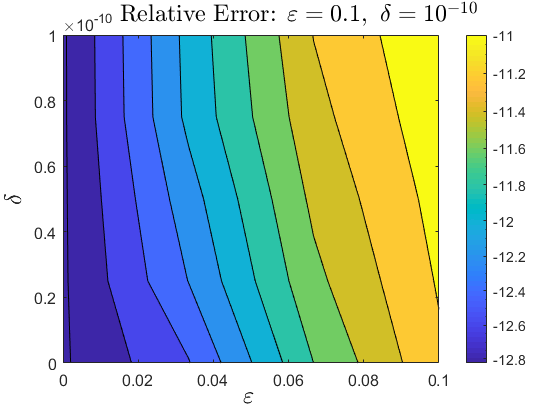
\includegraphics[width=7.6cm]{sections/7_conclusions_and_future_directions/Large_Eps_Small_Delta_2.png} }}%
    %\qquad
    \subfloat[\centering Small $\varepsilon$, Large $\delta$ ]{{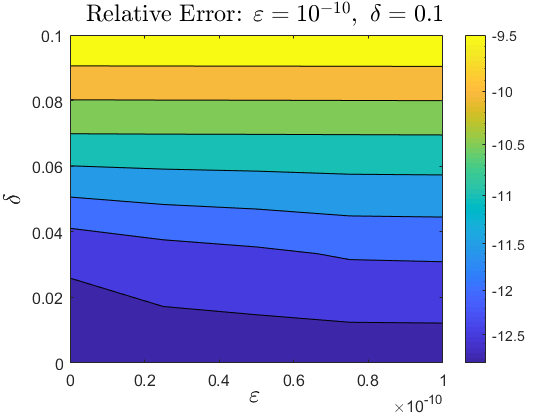
\includegraphics[width=7.6cm]{sections/7_conclusions_and_future_directions/Small_Eps_Large_Delta_2.png} }}%
    \vspace{3 mm}
    \caption{A contour plot of the relative error computed with our HOPS/AWE algorithm by holding $N=M=8$ Taylor orders fixed. In Figure $34\text{(a)}$ we expand up to $\Eps = 0.1$ and $\delta = 10^{-10}$ simultaneously with $N=M=8$ Taylor orders. In Figure $34\text{(b)}$ we expand up to $\Eps = 10^{-10}$ and $\delta = 0.1$ simultaneously with $N=M=8$ Taylor orders.}%
    \label{fig:example}%
\end{figure}
\vspace{-18mm}
Supplementary testing in both the upper and lower layers confirms that our HOPS/AWE algorithm is better suited towards larger $\varepsilon$.
%\begin{flushleft}
\newline
\\
\textbf{Predictions:} Our HOPS/AWE methodology takes advantage of exact enforcement of the \gls{owc} at an artificial boundary in order to truncate the computational domain to one of finite extent. After flattening the surface, the DNOs recover information through the solution stored at the interface. We suspect that this process mitigates large perturbations of the height/slope. By following techniques developed in \cite{NichollsReitich00b,NichollsTaber06,Nicholls16b,NichollsShen08}, we intend to rigorously prove that the TFE method is analytic when $\varepsilon$ is large. Additionally, we are interested in perturbing other physical parameters in the context of layered media problems. These are discussed in the engineering literature \cite{mashayekh2018parameter,mashayekh2018parameter2}.
\section{Rayleigh Singularities}
\label{Sec: Rayleigh Singularities}
A fundamental equation in the HOPS/AWE algorithm is
$$\alpha_p^2 + (\gamma_p^q(\delta))^2 = (k^q)^2,$$
where $k^q$ represents the wavenumber, $q\in\{u,w\}$, and $\alpha=k^q\sin(\theta), \gamma=k^q\cos(\theta),$ are parameters corresponding to refraction/reflection of the incidence angle $\theta$. As shown in $\S 5.4$, a Rayleigh singularity (or Wood's anomaly) occurs when $\ualpha_p^2 = (\uk^q)^2$ for any integer $p\neq 0$. That is, if $\ugamma_p^q(\delta) =0$ for $p\neq 0$ then the Taylor series expansion of $\gamma_p^q(\delta)$ is invalid. In \cite{Nicholls16}, the author investigated changing the Taylor expansion to a Puiseux expansion \cite{basu2007algorithms}:
$$\gamma_p^q(\delta)=\sum_{m=0}^{\infty}\gamma_{p,m}^q\delta^{m+1/2}=\delta^{1/2}\sum_{m=0}^{\infty}\gamma_{p,m}^q\delta^m.$$
However, he found that this approach ran into external difficulties ($\S$6 of \cite{Nicholls16}) simplifying explicit forms of the Dirichlet and Neumann trace operators.
\newline
\\
\textbf{Predictions:} Rayleigh singularities are a central obstruction to the convergence of our HOPS/AWE algorithm. In all of our numerical tests, we select custom frequency ranges which maximize the radius of convergence of our algorithm by expanding away from the singularities (cf. $\S 5.6$). Alternative methods such as Padé summation also fail to be analytic in a neighborhood of a Rayleigh singularity. General perturbation theory provides a variety of known techniques \cite{suslov2005divergent,convfromdiv,Heinz2020,dienes1957taylor,arteca1984summation} for expanding around divergent perturbation series. We suspect that adding these techniques to our HOPS/AWE algorithm will allow us perform a series expansion of $\ugamma_p^q(\delta)$ that does not diverge when $\ugamma_p^q(\delta)=0.$
\section{Multiple Layers}
\label{Sec: Multiple Layers}

In \cite{Nicholls16b}, the author discusses how to apply our HOPS methodology in multilayered configurations. He considers a multilayered material with $M$ (finite) interfaces at 
$$z=a^{(m)}+g^{(m)}(x,y),\quad 1\leq m \leq M,$$
which are $d_x \times d_y$ periodic
$$g^{(m)}(x+d_x,y+d_y)=g^{(m)}(x,y),\quad 1\leq m \leq M,$$
separating $(M+1)$--many layers.
%\vspace{-12mm}
\begin{figure}[H]
    \centering
    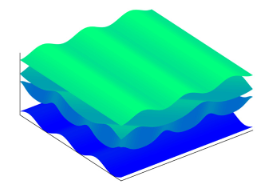
\includegraphics[width=7.6cm]{sections/7_conclusions_and_future_directions/multilayered.png}%
    \vspace{3mm}
    \caption{A five--layer problem configuration with layer interfaces $z = a^{(m)}+g^{(m)}(x).$}%
    \label{fig:example}%
\end{figure}
\vspace{-15mm}
%\begin{flushleft}
A generalization of our analyticity theorems (cf. $\S 4.5$) up to $M$ parameters is included as Theorem~$3.2$ in \cite{Nicholls16b}. For this, we consider quite general systems of linear equations of the form
%\end{flushleft}
\be
\bA(\tEps)\bV(\tEps)=\bR(\tEps),
\ee
where 
\bes
\bA(\tEps)=\sum_{\tn=0}^{\infty}\bA_{\tn}\tEps^{\tn},\quad 
\bR(\tEps) = \sum_{\tn=0}^{\infty}\bR_{\tn}\tEps^{\tn}.
\ees
The tildes represent multi--index notation \cite{Evans10}, in particular
\bes
\tEps := \begin{pmatrix} \Eps_1 \\ \vdots \\ \Eps_M \end{pmatrix},
\quad
\tn := \begin{pmatrix} n_1 \\ \vdots \\ n_M \end{pmatrix},
\ees
and the convention
\bes
\sum_{\tn=0}^{\infty} 
    A_{\tn}\ \tEps^{\tn}
  = \sum_{n_1=0}^{\infty} \cdots \sum_{n_M=0}^{\infty}
    A_{n_1,\ldots,n_M} \Eps_1^{n_1} \cdots \Eps_M^{n_M}.
\ees
As in $\S 4.5$, we seek a solution of the form
\be
\bV(\tEps)=\sum_{\tn=0}^{\infty}\bV_{\tn}\tEps^{\tn},
\ee
and from $(7.1)$ we find at order $\mathcal{O}(\tEps^{\tn})$
\bes
\bA_0\bV_{\tn}= \bR_{\tn} - \left(\sum_{\tl=0}^{\tn}\bA_{\tn-\tl}\bV_{\tl}- \bA_0\bV_{\tn}\right),
\ees
or
\be
\bV_{\tn}= \bA_0^{-1}\left\{\bR_{\tn} - \left(\sum_{\tl=0}^{\tn}\bA_{\tn-\tl}\bV_{\tl}- \bA_0\bV_{\tn}\right)\right\}.
\ee
The above notation represents multi--indices in the form
\bes
\sum_{\tl=0}^{\tn}\bA_{\tn-\tl}\bV_{\tl} = \sum_{\ell_1=0}^{n_1}\cdots \sum_{\ell_M=0}^{n_M}
    \bA_{n_1-\ell_1,\ldots,n_M-\ell_M} \bV_{\ell_1,\ldots,\ell_m},  
\ees
where $\tn=(n_1,\ldots,n_M),$ $\tl=(\ell_1,\ldots,\ell_M),$ and $0=(0,\ldots,0)$ with the convention
\bes
\tn \geq 0 \iff n_1\geq 0,\ldots,n_M\geq 0, \quad\tl \geq 0 \iff \ell_1\geq 0,\ldots,\ell_M\geq 0.
\ees
With these, we can extend our existence theorem (Theorem $4.5.1$) to $M$ parameters.
\begin{theorem}
\label{Thm:AVR}
Given two Banach spaces, $X$ and $Y$, suppose that:
\begin{enumerate}[label={\upshape[\arabic*]}]
\item $\bR_{\tn} \in Y$ for all $\tn \geq 0$,
  and there exist $M$--multi--indexed constants $C_R > 0$, $B_R > 0$,
  \bes
  C_R = \begin{pmatrix} C_{R,1} \\ \vdots \\ C_{R,M} \end{pmatrix},
  \quad
  B_R^{\tn} = \begin{pmatrix} B_{R,1}^{n_1} \\ \vdots \\ 
  B_{R,M}^{n_M} \end{pmatrix},
  \ees
  such that
  \bes
  \Norm{\bR_{\tn}}{Y} \leq C_R B_R^{\tn},
  \ees
\item $\bA_{\tn}: X \rightarrow Y$ for all
  $\tn \geq 0$, and there exist $M$--multi--indexed
  constants $C_A > 0$, $B_A > 0$ such that
  \bes
  \Norm{\bA_{\tn}}{X \rightarrow Y} \leq C_A B_A^{\tn},
  \ees
\item $\bA_0^{-1}: Y \rightarrow X$, and there 
  exists a constant $C_e > 0$ such that
  \bes
  \Norm{\bA_0^{-1}}{Y \rightarrow X} \leq C_e.
  \ees  
\end{enumerate}
Then the equation $(7.1)$ has a unique solution,
\be
\label{Eqn:V:Exp:Multi}
\bV(\tEps) = \sum_{\tn=0}^{\infty} \bV_{\tn} \tEps^{\tn},
\ee
and there exist $M$--multi--indexed constants $C_V > 0$ and $B_V > 0$ such that
\bes
\Norm{\bV_{\tn}}{X} \leq C_V B_V^{\tn},
\ees
for all $\tn \geq 0$ and any
\bes
C_V \geq 2 C_e C_R,
\quad
B_V \geq \max \left\{ B_R, 2 B_A, 2^{M+1} C_e C_A B_A \right\},
\ees
enforced componentwise. This implies that, for any $M$--multi--indexed constant
$0 \leq \tilde{\rho} < 1$, 
$(7.4)$, converges for all $\tEps$ such that
$B \tEps < \tilde{\rho}$, i.e., $\tEps < \tilde{\rho}/B$.
\end{theorem}
\begin{remark}
Our proof strategy is a form of multidimensional induction where given a statement $\bP(n_1, n_2, n_3, ..., n_M)$ for some $M\in \mathbb{N}$, we will show that $\forall n_1, n_2,\ldots, n_M \geq 0$, $\bP(n_1, n_2, n_3, ..., n_M)$ is true by inducting on $n_M$. We will follow the steps outlined below.
\begin{enumerate}
\item Establish $\bP(0,\ldots,n_j,\ldots,0)$ for all $1 \leq j < M$ and $n_1,\ldots,n_j \geq 0.$
\item Given $\bP(n_1,n_2,\ldots,n_j,\ldots,0)$ for all $1 \leq j < M$ and $n_1,\ldots,n_j \geq 0$, establish $\bP(n_1,n_2,\ldots,\bar{n}_j,\ldots,0)$. This can be accomplished through the two steps below.
\begin{enumerate}
    \item Establish $\bP(0,\ldots,\bar{n}_j,\ldots,0)$ for all $\bar{n}_j \geq 0$ (where the hypothesis in $[2]$ gives the required case for $n_j < \bar{n}_j$).
    \item Given  $\bP(n_1,n_2,\ldots,\bar{n}_j,\ldots,0)$ for all $1 \leq j < M$ and $n_1 < \bar{n}_1,  n_2 < \bar{n}_2,\ldots, $ $n_{j-1}  < \bar{n}_{j-1}$ and $\bar{n}_j\geq 0$, establish $\bP(\bar{n}_1,\bar{n}_2,\ldots,\bar{n}_j,\ldots,0)$.
\end{enumerate}
\item Given $\bP(n_1,n_2,\ldots,n_j,n_{j+1},\ldots,0)$ for all $1 \leq j+1 < M$ and $n_1,\ldots,n_{j+1} \geq 0$, establish $\bP(n_1,n_2,\ldots,n_j,\bar{n}_{j+1},\ldots,0)$. This can be accomplished by following the two steps outlined below. 
\begin{enumerate}
    \item Establish $\bP(0,\ldots,\bar{n}_{j+1},\ldots,0)$ for all $\bar{n}_{j+1} \geq 0$ (where the hypothesis in $[3]$ gives the required case for $n_{j+1} < \bar{n}_{j+1}$).
    \item Given  $\bP(n_1,n_2,\ldots,n_j,\bar{n}_{j+1},\ldots,0)$ for all $1 \leq j+1 < M$ and  $n_1 < \bar{n}_1,  n_2 < \bar{n}_2,\ldots, n_{j} < \bar{n}_{j}$ and $\bar{n}_{j+1}\geq 0$, establish $\bP(\bar{n}_1,\bar{n}_2,\ldots,\bar{n}_j,\bar{n}_{j+1}\ldots,0)$.
\end{enumerate}
\item Given $\bP(n_1,n_2,\ldots,n_{M-1},n_M)$ for all $n_1,n_2,\ldots,n_{M-1} \geq 0$ and $n_M < \bar{n}_M$, establish $\bP(n_1,n_2,\ldots,n_{M-1},\bar{n}_M)$. This can be accomplished by the two steps below (the base cases are handled through $[2]$ and $[3]$).
\begin{enumerate}
    \item Establish $\bP(0,\ldots,\bar{n}_{M})$ for $\bar{n}_{M} \geq 0$ (where the hypothesis in $[4]$ handles the required case for  $n_{M} < \bar{n}_{M}$).
    \item Given $\bP(n_1,n_2,\ldots,n_{M-1},\bar{n}_M)$ for all $n_1 < \bar{n}_1, n_2 < \bar{n}_2, \ldots n_{M-1} < \bar{n}_{M-1}$ and $\bar{n}_M \geq 0$, establish $\bP(\bar{n}_1,\bar{n}_2,\ldots,\bar{n}_{M-1},\bar{n}_M)$.
\end{enumerate}
\end{enumerate}

\end{remark}

\begin{proof}{[Theorem 7.4.1]} As with $\tEps$ and $\tn$, we represent $\tilde{\rho}$ by
\bes
\tilde{\rho} := \begin{pmatrix} \rho_1 \\ \vdots \\ \rho_M \end{pmatrix}.
\ees
As before, we will work by induction and consider the general case for finite $M>0$ where we want to establish
\bes
\norm{\bV_{n_1,\ldots,n_M}}_X \leq C_{V,1}\ldots C_{V,M} B_{V,1}^{n_1}\ldots B_{V,M}^{n_M}, \quad \forall n_1,\ldots,n_M\geq 0.
\ees
We prove this via an induction on $n_M$. The base case $n_1,n_2,\ldots, n_{j-1},n_{j+1},\ldots,$ $n_M=0$ and $1 \leq j < M$:
\bes
\norm{\bV_{0,\ldots,n_j,\ldots,0}}_X \leq C_{V,j} B_{V,j}^{n_j}, \quad \forall n_j\geq 0,
\ees
has previously been established by Theorem $4.5.1$ where $\tEps = \Eps_j$ and $\delta=0$. We now assume
\bes
\norm{\bV_{n_1,\ldots,n_j,\ldots,0}}_X \leq  C_{V,1}\ldots C_{V,j}B_{V,1}^{n_1}\ldots B_{V,j}^{n_j}, ~~ \forall n_1,\ldots,n_{j-1}\geq 0,~~ \forall n_j < \bar{n}_j,~~ 1 \leq j < M,
\ees
and seek
\bes
\norm{\bV_{n_1,\ldots,\bar{n}_j,\ldots,0}}_X \leq  C_{V,1}\ldots C_{V,j}B_{V,1}^{n_1}\ldots B_{V,j}^{\bar{n}_j}, ~~ \forall n_1,\ldots,n_{j-1}\geq 0.
\ees
This can be obtained through a chain of $(M-1)$ inductions on $n_1,\ldots,n_j$ where $1 \leq j < M$. For simplicity, we will show what happens in the arbitrary case $n_j$. The base case $n_1,\ldots,n_{j-1}=0$:
\bes
\norm{\bV_{0,\ldots,\bar{n}_j,\ldots,0}}_X \leq  C_{V,j}B_{V,j}^{\bar{n}_j}, \quad \forall \bar{n}_j \geq 0,
\ees
is established by Theorem $4.5.1$ where $\tEps = \Eps_j$ and $\delta=0$. Therefore, we assume
\begin{align*}
\norm{\bV_{n_1,\ldots,\bar{n}_j,\ldots,0}}_X \leq  C_{V,1}\ldots C_{V,j}B_{V,1}^{n_1}\ldots B_{V,j}^{\bar{n}_j},~~\forall n_1  &< \bar{n}_1,\ldots, n_{j-1} < \bar{n}_{j-1},~~ \forall \bar{n}_j \geq 0,\\&~ 1 \leq j < M,
\end{align*}
and seek
\bes
\norm{\bV_{\bar{n}_1,\ldots,\bar{n}_j,\ldots,0}}_X \leq  C_{V,1}\ldots C_{V,j}B_{V,1}^{\bar{n}_1}\ldots B_{V,j}^{\bar{n}_j}.
\ees
Recalling $\tn=(n_1,\ldots,n_j)$ and  $\tl=(\ell_1,\ldots,\ell_j)$, we define
\be
{\sum_{\tl=0}^{\tn}}^{*}\bA_{\tn-\tl}\bV_{\tl} := \sum_{\tl=0}^{\tn}\bA_{\tn-\tl}\bV_{\tl} - \bA_0\bV_{\tn},
\ee
and apply $(7.3),(7.5)$ and the mapping properties of $\bA_{0}^{-1}$ to find
\bes
\norm{\bV_{\bar{n}_1,\ldots,\bar{n}_j,\ldots,0}}_X\leq C_e\left\{\norm{\bR_{\bar{n}_1,\ldots,\bar{n}_j}}_Y + {\sum_{\tl=0}^{\tn}}^{*}\norm{\bA_{\tn-\tl}\bV_{\tl}}_Y\right\}.
\ees
Using the estimates on $\bR_{n_1,\ldots,n_j}$ and $\bA_{n_1,\ldots,n_j}$ (for all $n_1,\ldots,n_j$) and $\bV_{n_1,\ldots,n_j}$ $(n_1 < \bar{n}_1, \ldots, n_j < \bar{n}_j)$ we have
\begin{align*}
\norm{\bV_{\bar{n}_1,\ldots,\bar{n}_j,\ldots,0}}_X &\leq
C_e\Bigg\{C_{R,1}\ldots C_{R,j}B_{R,1}^{\bar{n}_1}\ldots B_{R,j}^{\bar{n}_j} + {\sum_{\tl=0}^{\tn}}^{*}C_{A,1}\ldots C_{A,j}B_{A,1}^{\bar{n}_1-\ell_1}\ldots B_{A,j}^{\bar{n}_j-\ell_j}\\ & \qquad \qquad \qquad \qquad \qquad \qquad \qquad \qquad \times
C_{V,1}\ldots C_{V,j}B_{V,1}^{\ell_1}\ldots B_{V,j}^{\ell_j}\Bigg\} \\& =
C_eC_{R,1}\ldots C_{R,j}B_{R,1}^{\bar{n}_1}\ldots B_{R,j}^{\bar{n}_j} + C_eC_{A,1}\ldots C_{A,j}C_{V,1}\ldots C_{V,j} \\&
~~ \times \left(\frac{B_{A,1}}{B_{V,1}}\right)B_{V,1}^{\bar{n}_1}\cdots \left(\frac{B_{A,j}}{B_{V,j}}\right)B_{V,j}^{\bar{n}_j}{\sum_{\tl=0}^{\tn}}^{*}
\left(\frac{B_{A,1}}{B_{V,1}}\right)B_{V,1}^{\bar{n}_1-\ell_1-1}\cdots \\& ~~ \times
\left(\frac{B_{A,j}}{B_{V,j}}\right)B_{V,j}^{\bar{n}_j-\ell_j-1} \\& \leq
C_eC_{R,1}\ldots C_{R,j}B_{V,1}^{\bar{n}_1}\ldots B_{V,j}^{\bar{n}_j} + C_eC_{A,1}\ldots C_{A,j}C_{V,1}\ldots C_{V,j} \\& ~~ \times
\left(\frac{B_{A,1}}{B_{V,1}}\right)B_{V,1}^{\bar{n}_1}\cdots\left(\frac{B_{A,j}}{B_{V,j}}\right)B_{V,j}^{\bar{n}_j}\left(\frac{1}{1-1/2}\right)^j,
\end{align*}
if $B_{A,k}/B_{V,k} \leq 1/2$, $k=1,\ldots,j$ (implying $B_{V,k} \geq 2B_{A,k}$). We are done if we demand that
\bes
B_{V,k} \geq B_{R,k}, \quad C_eC_{R,k} \leq C_{V,k}/2, \quad 2^jC_eC_{A,k}C_{V,k}(B_{A,k}/B_{V,k}) \leq 
C_{V,k}/2.
\ees
This can be realized if
\bes
C_{V,k} \geq 2C_eC_{R,k}, \quad
B_{V,k} \geq \max\left\{B_{R,k},2B_{A,k},2^{j+1}C_eC_{A,k}B_{A,k}\right\}.
\ees
We then assume
\begin{align*}
\norm{\bV_{n_1,\ldots,n_{j+1},\ldots,0}}_X \leq  C_{V,1}\ldots C_{V,j+1}B_{V,1}^{n_1}\ldots B_{V,j+1}^{n_{j+1}}, ~~ &\forall n_1,\ldots,n_j\geq 0,~~ \forall n_{j+1} < \bar{n}_{j+1},\\&~~ 1 \leq j < M,
\end{align*}
and seek
\bes
\norm{\bV_{n_1,\ldots,\bar{n}_{j+1},\ldots,0}}_X \leq  C_{V,1}\ldots C_{V,j+1}B_{V,1}^{n_1}\ldots B_{V,j+1}^{\bar{n}_{j+1}}, ~~ \forall n_1,\ldots,n_{j}\geq 0.
\ees
As before, this can be obtained through a chain of $M$ inductions on $n_1,\ldots,n_{j+1}$ where $1 \leq j < M$. For simplicity, we will show what happens in the arbitrary case $n_{j+1}$. The base case $n_1,\ldots,n_{j}=0$:
\bes
\norm{\bV_{0,\ldots,\bar{n}_{j+1},\ldots,0}}_X \leq  C_{V,j+1}B_{V,j+1}^{\bar{n}_{j+1}}, \quad \forall \bar{n}_{j+1} \geq 0,
\ees
is established by Theorem $4.5.1$ where $\tEps = \Eps_{j+1}$ and $\delta=0$. Therefore, we assume
\begin{align*}
\norm{\bV_{n_1,\ldots,\bar{n}_{j+1},\ldots,0}}_X \leq  C_{V,1}\ldots C_{V,j+1}B_{V,1}^{n_1}\ldots B_{V,j+1}^{\bar{n}_{j+1}},~~\forall n_1  &< \bar{n}_1,\ldots, n_{j} < \bar{n}_{j},~~ \forall \bar{n}_{j+1} \geq 0,\\&~ 1 \leq j < M,
\end{align*}
and seek
\bes
\norm{\bV_{\bar{n}_1,\ldots,\bar{n}_{j+1},\ldots,0}}_X \leq  C_{V,1}\ldots C_{V,j+1}B_{V,1}^{\bar{n}_1}\ldots B_{V,j+1}^{\bar{n}_{j+1}}.
\ees
In this scenario, $\tn=(n_1,\ldots,n_{j+1})$ and  $\tl=(\ell_1,\ldots,\ell_{j+1}),$ so we apply $(7.3),(7.5)$ and the mapping properties of $\bA_{0}^{-1}$ to find
\bes
\norm{\bV_{\bar{n}_1,\ldots,\bar{n}_{j+1},\ldots,0}}_X\leq C_e\left\{\norm{\bR_{\bar{n}_1,\ldots,\bar{n}_{j+1}}}_Y + {\sum_{\tl=0}^{\tn}}^{*}\norm{\bA_{\tn-\tl}\bV_{\tl}}_Y\right\}.
\ees
Using the estimates on $\bR_{n_1,\ldots,n_{j+1}}$ and $\bA_{n_1,\ldots,n_{j+1}}$ (for all $n_1,\ldots,n_{j+1}$) and $\bV_{n_1,\ldots,n_{j+1}}$ $(n_1 < \bar{n}_1, \ldots, n_{j+1} < \bar{n}_{j+1})$ we have
\begin{align*}
\norm{\bV_{\bar{n}_1,\ldots,\bar{n}_{j+1},\ldots,0}}_X &\leq
C_e\Bigg\{C_{R,1}\ldots C_{R,{j+1}}B_{R,1}^{\bar{n}_1}\ldots B_{R,{j+1}}^{\bar{n}_{j+1}} + {\sum_{\tl=0}^{\tn}}^{*}C_{A,1}\ldots C_{A,{j+1}}B_{A,1}^{\bar{n}_1-\ell_1}\ldots \\ & \qquad \qquad \qquad \qquad \qquad \quad \times
B_{A,{j+1}}^{\bar{n}_{j+1}-\ell_{j+1}}C_{V,1}\ldots C_{V,{j+1}}B_{V,1}^{\ell_1}\ldots B_{V,{j+1}}^{\ell_{j+1}}\Bigg\} \\& =
C_eC_{R,1}\ldots C_{R,{j+1}}B_{R,1}^{\bar{n}_1}\ldots B_{R,{j+1}}^{\bar{n}_{j+1}} + C_eC_{A,1}\ldots C_{A,{j+1}}C_{V,1}\ldots C_{V,{j+1}} \\&
~~ \times \left(\frac{B_{A,1}}{B_{V,1}}\right)B_{V,1}^{\bar{n}_1}\cdots \left(\frac{B_{A,{j+1}}}{B_{V,{j+1}}}\right)B_{V,{j+1}}^{\bar{n}_{j+1}}{\sum_{\tl=0}^{\tn}}^{*}
\left(\frac{B_{A,1}}{B_{V,1}}\right)B_{V,1}^{\bar{n}_1-\ell_1-1}\cdots \\& ~~ \times
\left(\frac{B_{A,{j+1}}}{B_{V,{j+1}}}\right)B_{V,{j+1}}^{\bar{n}_{j+1}-\ell_{j+1}-1} \allowdisplaybreaks\\& \leq
C_eC_{R,1}\ldots C_{R,{j+1}}B_{V,1}^{\bar{n}_1}\ldots B_{V,{j+1}}^{\bar{n}_{j+1}} + C_eC_{A,1}\ldots C_{A,{j+1}}C_{V,1}\ldots C_{V,{j+1}} \\& ~~ \times
\left(\frac{B_{A,1}}{B_{V,1}}\right)B_{V,1}^{\bar{n}_1}\cdots\left(\frac{B_{A,{j+1}}}{B_{V,{j+1}}}\right)B_{V,{j+1}}^{\bar{n}_{j+1}}\left(\frac{1}{1-1/2}\right)^{j+1},
\end{align*}
if $B_{A,t}/B_{V,t} \leq 1/2$, $t=1,\ldots,j+1$ (implying $B_{V,t} \geq 2B_{A,t}$). We are done if we demand that
\bes
B_{V,t} \geq B_{R,t}, \quad C_eC_{R,t} \leq C_{V,t}/2, \quad 2^{j+1}C_eC_{A,t}C_{V,t}(B_{A,t}/B_{V,t}) \leq 
C_{V,t}/2.
\ees
This can be realized if
\bes
C_{V,t} \geq 2C_eC_{R,t}, \quad
B_{V,t} \geq \max\left\{B_{R,t},2B_{A,t},2^{j+2}C_eC_{A,t}B_{A,t}\right\}.
\ees
To complete the general case for finite $M>0$, we assume
\bes
\norm{\bV_{n_1,\ldots,n_M}}_X \leq  C_{V,1}\ldots C_{V,M}B_{V,1}^{n_1}\ldots B_{V,M}^{n_M}, ~~ \forall n_1,\ldots,n_{M-1}\geq 0,~~ \forall n_M < \bar{n}_M,
\ees
and seek
\bes
\norm{\bV_{n_1,\ldots,\bar{n}_M}}_X \leq  C_{V,1}\ldots C_{V,M}B_{V,1}^{n_1}\ldots B_{V,M}^{\bar{n}_M}, ~~ \forall n_1,\ldots,n_{M-1}\geq 0.
\ees
The base case $n_1,n_2,\ldots,n_{M-1}=0$:
\bes
\norm{\bV_{0,\ldots,\bar{n}_M}}_X \leq  C_{V,M}B_{V,M}^{\bar{n}_M}, \quad \forall \bar{n}_M \geq 0,
\ees
has previously been established by Theorem $4.5.1$ where $\tEps = \Eps_M$ and $\delta =0$. Finally, we assume
\begin{align*}
\norm{\bV_{n_1,\ldots,n_{M-1},\bar{n}_M}}_X \leq  C_{V,1}\ldots C_{V,M}B_{V,1}^{n_1}\ldots B_{V,M}^{\bar{n}_M},~~~&\forall n_1  < \bar{n}_1,\ldots, n_{M-1} < \bar{n}_{M-1},\\&~~~~ \forall \bar{n}_M \geq 0,
\end{align*}
and seek
\bes
\norm{\bV_{\bar{n}_1,\ldots,\bar{n}_{M-1},\bar{n}_M}}_X \leq  C_{V,1}\ldots C_{V,M}B_{V,1}^{\bar{n}_1}\ldots B_{V,M}^{\bar{n}_M}.
\ees
In this case, $\tn=(n_1,\ldots,n_M)$ and  $\tl=(\ell_1,\ldots,\ell_M),$ so we apply $(7.3),(7.5)$ and the mapping properties of $\bA_{0}^{-1}$ to find
\bes
\norm{\bV_{\bar{n}_1,\ldots,\bar{n}_M}}_X\leq C_e\left\{\norm{\bR_{\bar{n}_1,\ldots,\bar{n}_M}}_Y + {\sum_{\tl=0}^{\tn}}^{*}\norm{\bA_{\tn-\tl}\bV_{\tl}}_Y\right\}.
\ees
Using the estimates on $\bR_{n_1,\ldots,n_M}$ and $\bA_{n_1,\ldots,n_M}$ (for all $n_1,\ldots,n_M$) and $\bV_{n_1,\ldots,n_M}$ $(n_1 < \bar{n}_1, \ldots, n_M < \bar{n}_M)$ we have
\vspace{-1.5mm}
\begin{align*}
\norm{\bV_{\bar{n}_1,\ldots,\bar{n}_M}}_X &\leq
C_e\Bigg\{C_{R,1}\ldots C_{R,M}B_{R,1}^{\bar{n}_1}\ldots B_{R,M}^{\bar{n}_M} + {\sum_{\tl=0}^{\tn}}^{*}C_{A,1}\ldots C_{A,M}B_{A,1}^{\bar{n}_1-\ell_1}\ldots B_{A,M}^{\bar{n}_M-\ell_M}\\ & \qquad \qquad \qquad \qquad \qquad \qquad \qquad \qquad \times
C_{V,1}\ldots C_{V,M}B_{V,1}^{\ell_1}\ldots B_{V,M}^{\ell_M}\Bigg\} \\& =
C_eC_{R,1}\ldots C_{R,M}B_{R,1}^{\bar{n}_1}\ldots B_{R,M}^{\bar{n}_M} + C_eC_{A,1}\ldots C_{A,M}C_{V,1}\ldots C_{V,M} \\& 
~~ \times \left(\frac{B_{A,1}}{B_{V,1}}\right)B_{V,1}^{\bar{n}_1}\cdots \left(\frac{B_{A,M}}{B_{V,M}}\right)B_{V,M}^{\bar{n}_M}{\sum_{\tl=0}^{\tn}}^{*}
\left(\frac{B_{A,1}}{B_{V,1}}\right)B_{V,1}^{\bar{n}_1-\ell_1-1}\cdots \\& \allowdisplaybreaks~~ \times
\left(\frac{B_{A,M}}{B_{V,M}}\right)B_{V,M}^{\bar{n}_M-\ell_M-1} \\&  \leq
C_eC_{R,1}\ldots C_{R,M}B_{V,1}^{\bar{n}_1}\ldots B_{V,M}^{\bar{n}_M} + C_eC_{A,1}\ldots C_{A,M}C_{V,1}\ldots C_{V,M} \\& ~~ \times
\left(\frac{B_{A,1}}{B_{V,1}}\right)B_{V,1}^{\bar{n}_1}\cdots\left(\frac{B_{A,M}}{B_{V,M}}\right)B_{V,M}^{\bar{n}_M}\left(\frac{1}{1-1/2}\right)^M,
\end{align*}
if $B_{A,i}/B_{V,i} \leq 1/2$, $i=1,\ldots,M$ (implying $B_{V,i} \geq 2B_{A,i}$). We are done if we demand that
\bes
B_{V,i} \geq B_{R,i}, \quad C_eC_{R,i} \leq C_{V,i}/2, \quad 2^MC_eC_{A,i}C_{V,i}(B_{A,i}/B_{V,i}) \leq 
C_{V,i}/2.
\ees
This can be realized if
\bes
C_{V,i} \geq 2C_eC_{R,i}, \quad
B_{V,i} \geq \max\left\{B_{R,i},2B_{A,i},2^{M+1}C_eC_{A,i}B_{A,i}\right\}.
\ees
\end{proof}
Using a similar approach in conjunction with the analysis in Chapters $2$ and $3$, we predict a more general form of Theorems $2.9.2$ and $3.8.1$ exists, which would establish the analyticity of the transformed field with respect to any finite $M > 0$ perturbation parameters.
\vspace{1mm}
\begin{conjecture} 
\label{Conj:u,w:Anal:n:n_m}
Given any integer $s \geq 0$, if $f \in C^{s+2}([0,d])$ and 
$U_{\tilde{n}} \in H^{s+3/2}([0,d])$, $W_{\tilde{n}}\in H^{s+3/2}([0,d])$ such that
\bes
\|U_{\tilde{n}}\|_{H^{s+3/2}} \le K_U B_U^{\tn} , \quad
\|W_{\tilde{n}}\|_{H^{s+3/2}} \le K_W B_W^{\tn} ,
\ees
for constants $K_U, K_W>0$ and $M$--multi--indexed constants $B_U, B_W > 0$, then 
$u_{\tn} \in H^{s+2}([0,d]\times[0,a])$, $w_{\tn}\in H^{s+2}([0,d]\times[-b,0])$ and
\bes
\label{Eqn:u,w:Est:n:n_m}
\|u_{\tn}\|_{H^{s+2}} \le K B^{\tn}, \quad
\|w_{\tn}\|_{H^{s+2}} \le \tilde{K}\tilde{B}^{\tn} ,
\ees
for constants $K,\tilde{K}> 0$ and $M$--multi--indexed constants $B ,\tilde{B}>0$.
\end{conjecture}
\vspace{1mm}
Analogously, a similar procedure would establish a more general form of Theorems $2.10.2$ and $3.9.2$ for the analyticity of the DNOs for any finite $M>0$ perturbation parameters.
\vspace{1mm}
\begin{conjecture} 
\label{Thm:G,J:Anal:n:n_m}
Given any integer $s \geq 0$, if $f \in C^{s+2}([0,d])$ and 
$U_{\tn} \in H^{s+3/2}([0,d])$, $W_{\tn} \in H^{s+3/2}([0,d])$ such that
\bes
\SobNorm{U_{\tn}}{s+3/2} \leq K_U B_U^{\tn}, \quad
\SobNorm{W_{\tn}}{s+3/2} \leq K_W B_W^{\tn},
\ees
for constants $K_U,K_W> 0$ and $M$--multi--indexed constants $B_U, B_W > 0$, then $G_{\tn} \in H^{s+1/2}([0,d])$, $J_{\tn} \in H^{s+1/2}([0,d])$ and
\bes
\label{Eqn:G,J:Est:n:n_m} 
\|G_{\tn}\|_{H^{s+1/2}} \le \tilde{K}\tilde{B}^{\tn}, \quad
\|J_{\tn}\|_{H^{s+1/2}} \le \dbtilde{K} \dbtilde{B}^{\tn},
\ees
for constants $\tilde{K},\dbtilde{K}  > 0$ and $M$--multi--indexed constants $\tilde{B},\dbtilde{B}>0$.
\end{conjecture}
\vspace{1mm}
Upon proving these, one has two key ingredients to the more general version of Theorem $4.6.1$ which establishes the existence and uniqueness of solutions to a system of partial differential equations with respect to $M$ perturbation parameters.
\vspace{1mm}
\begin{conjecture} 
\label{Conj:Main}
Given an integer $s \geq 0$, if $f \in C^{s+2}([0,d])$ then the 
equation $(7.1)$ has a unique solution, $(7.4)$,
and there exist a constant $C > 0$ and $M$--multi--indexed constants $B>0$ such that
\bes
\Norm{\bV_{\tn}}{X^s} \leq C B^{\tn},
\ees
for all $\tn \geq 0$.  This implies that for any $M$--multi--indexed constant
$0 \leq \tilde{\rho} < 1$, $(7.4)$, converges for all $\tEps$ such that
$B \tEps < \tilde{\rho}$, i.e., $\tEps < \tilde{\rho}/B$.
\end{conjecture}
\vspace{1mm}
\textbf{Predictions:} In application oriented fields such as signal processing or sea ice modeling, practitioners work with  multiple frequencies \cite{qiu2005high,bosse1995model,zhao2009multi,blanchard2021high} at short or long wavelengths. Also, as depicted in Figure $35$, the grating surface could have $M$ different layers \cite{imperatore2017perturbation} with distinct values of $g_j(x)=\Eps f_j(x),~j=1,\ldots, M$. A proof of Conjecture $7.4.4$ would enable the freedom to enforce any number of perturbation parameters and obtain an analytic solution. Given the widespread availability of parallel computing resources coupled with additional perturbation parameters associated with elastic media, we believe that future research will force hundreds or even thousands of distinct perturbation parameters, all of which should yield an analytic solution.
\section{Parallel Programming}
\setcounter{section}{5}
\label{Sec: Parallel Programming}

In the case of multiple layered interfaces, we need to compute intermediate DNOs for up to $M$ layers. This will greatly increase the computational cost and execution time of our HOPS/AWE algorithm and we suspect that it will be necessary to introduce parallel programming techniques to offset the computational expense. In the context of the \gls{oe} method, preliminary work \cite{fang2015operator} has been completed in C\texttt{++} to parallelize the computation of Navier's equations \cite{BillinghamKing00,achenbach2012wave}. These techniques can be adapted to the TFE method through the choice of OpenMP \cite{chandra2001parallel}, MPI \cite{snir1998mpi}, or CUDA \cite{sanders2010cuda}.
\newline
\\
\textbf{Predictions:} In two or three dimensions, our HOPS code is robust, efficient and has a runtime less than an hour. A local machine with an Intel Core i$5$ CPU, $8$GB of RAM, and Windows $10$ OS completed almost every simulation in this thesis in less than thirty minutes. However, with ten to one hundred layer configurations, we suspect that many simulations will take on the order of weeks or even months. As a result, it will be necessary to parallelize our Matlab code in a compiled programming language such as C or  C\texttt{++}.

\section{Alternatives to DNOs}
\label{Sec: Alternatives to DNOs}
In Chapter $4$ we wrote our scattering problem as a linear system
\bes
\bA \bV = \bR,
\ees
where, upon expanding $\{\bA,\bV,\bR\}$ in both $\varepsilon$ and $\delta$, we arrived at the flat--interface solution $\bA_{0,0}\bV_{0,0}=\bR_{0,0}$
at order $\mathcal{O}(\varepsilon^0,\delta^0)$. We then saw it was necessary to invert
\bes
\bA_{0,0} = \begin{pmatrix}I & -I\\
-G_{0,0} & -\tau^2J_{0,0}\end{pmatrix}, 
\ees
which features the two DNOs, $G_{0,0}$ and $J_{0,0}$, in order to show the existence and uniqueness of solutions. A primary feature of all HOPS schemes is the inversion of a single, sparse operator $\bA_{0,0}$ through the use of DNOs. However, one may ponder if a different technique could produce a more competitive algorithm that is comparable to our HOPS/AWE algorithm (or even better). Is it absolutely necessary to pass in transformed field data in order to efficiently compute and recover internal information stored at the grating surface?
\\
\newline
\textbf{Predictions:} A primary advantage of our HOPS/AWE scheme is that for every perturbation order, it is only necessary to invert a single sparse operator corresponding to a flat--interface, order--zero approximation. There are a number of competing approaches in general perturbation theory within the context of layered media problems. In regards to electromagnetic wave scattering, Galerkin and boundary element methods are discussed in \cite{escapil2020helmholtz,silva2017quantifying,nakata1990boundary,elschner2012optimization,rathsfeld2006} and a high--order perturbation approach based on boundary integral equations in \cite{dolz2020higher}. High--order schemes for linear waves can be computed using level set methods \cite{sethian1999level} and fast marching methods, as well as other methods involving domain decomposition \cite{el2004comparing,benamou1997domain,larsson1999domain,gong2021convergence,perez2018domain,chan1994domain}. A holistic evaluation of these competing methods could potentially improve our HOPS/AWE algorithm if we found a faster method of inverting linear operators without the use of DNOs.
\section{Computational Complexity}
\label{Sec: Computational Complexity}

One of the fundamental reasons for developing our HOPS/AWE algorithm is its advantageous computational complexity for problems within its domain of applicability.
In comparison with other classical methods, our HOPS/AWE approach has several advantages for computing quantities such as the Reflectivity Map, $R=R(\varepsilon,\delta)$. To demonstrate this we begin
by fixing the problem of computing $R$ for $N_{\Eps}$ many values of 
$\Eps$ and $N_{\delta}$ many values of $\delta$.

In the case of computing the DNOs $G$ and $J$, we recall from $\S 2.11$ and $\S 3.10$ that our HOPS/AWE algorithm requires
$N_x \times N_z$ unknowns at every perturbation order, $(n,m)$, corresponding to
the $N_x$ equally--spaced gridpoints in the lateral direction and the $N_z + 1$ collocation points in the vertical dimension. In $\S 4.5$ we saw that we could write our scattering problem as $\bA(\Eps,\delta) \bV(\Eps,\delta) = \bR(\Eps,\delta)$ where
\bes
    \bA(\Eps,\delta)=\sumn \summ \bA_{n,m}\Eps^n\delta^m, \quad \bR(\Eps,\delta) = \sumn \summ \bR_{n,m}\Eps^{n}\delta^m,
\ees
and
\bes
\label{Eqn:Soln:Two_Param_Append}
\bV(\Eps,\delta) = \sumn \summ \bV_{n,m}\Eps^{n}\delta^m.
\ees
At order $\mathcal{O}(\Eps^n,\delta^m)$ this becomes
\begin{align}
\begin{split}
\bA_{0,0}\bV_{n,m}=&~\bR_{n,m}-\sum_{\ell=0}^{n-1}\bA_{n-\ell,0}\bV_{\ell,m}-\sum_{r=0}^{m-1}\bA_{0,m-r}\bV_{n,r}\\&
-\sum_{\ell=0}^{n-1}\sum_{r=0}^{m-1}\bA_{n-\ell,m-r}\bV_{\ell,r}.
\end{split}
\end{align}
A careful study of $(7.6)$
reveals that the computational complexity of forming the
right--hand side at order $(n,m)$ is
\bes
\BigOh{n m N_x \log(N_x) N_z \log(N_z)}.
\ees
Inverting the operator $\bA_{0,0}$ has complexity $\BigOh{N_x \log(N_x) N_z \log(N_z)}$
so the full cost of computing the $\bV_{n,m}$, 
$\{ 0 \leq n \leq N, 0 \leq m \leq M \}$, is
\bes
\BigOh{N^2 M^2 N_x \log(N_x) N_z \log(N_z)}.
\ees
Once these coefficients are recovered, the cost of summing the series in 
$(\Eps,\delta)$ is minimal, provided it is done in an efficient manner 
(e.g., by Horner's rule \cite{BurdenFaires,AtkinsonHan01}). Our algorithm then 
requires an additional $\BigOh{N_{\Eps} N_{\delta}}$ steps to sum 
over every value of $(\Eps,\delta)$, therefore the full cost of 
computing the Reflectivity Map by our HOPS/AWE method is
\be
\BigOh{N^2 M^2 N_x \log(N_x) N_z \log(N_z) + N_{\Eps} N_{\delta}}.
\ee
In contrast, for a single $(\Eps,\delta)$ pair, a Boundary Integral Method solver with $N_x$ lateral
gridpoints requires time proportional to $\BigOh{N_x^3}$ for Gaussian elimination
to solve the resulting dense system of $N_x$ equations in $N_x$ unknowns
\cite{BurdenFaires,AtkinsonHan01,ColtonKress13}. Applying this 
$N_{\Eps} \times N_{\delta}$ times results in a total computational complexity of
\be
\BigOh{N_x^3 N_{\Eps} N_{\delta}}.
\ee
Thus, once $N_{\Eps}$ and $N_{\delta}$ become large, e.g.,

\bes
N_{\Eps} N_{\delta} > \frac{N^2 M^2 N_x \log(N_x) N_z \log(N_z)}{N_x^3},
\ees
our new algorithm becomes far more efficient. We speculate that the cost of $(7.7)$ could be reduced to
\be
\BigOh{N M \log(NM)N_x \log(N_x) N_z \log(N_z) + N_{\Eps} N_{\delta}},
\ee
provided that we develop a more efficient method of computing the $\bV_{n,m}$, 
$\{ 0 \leq n \leq N, 0 \leq m \leq M \}$, such as reducing the problem space at every step. Alternative approaches to layered media problems have also been proposed by other authors \cite{bai2004reduction,chew2005fast}, including interpolation \cite{atkins2010fast} and Green's function \cite{konno2016fast}.
\newline
\\
\textbf{Predictions:} The combination of implementing parallel programming techniques (through, e.g., OpenMP or CUDA) and reducing the problem space at every step will greatly enhance the speed and fidelity of our HOPS/AWE algorithm. Considering the natural advantage surface methods have over conventional methods, such as finite difference, finite element, and spectral element methods, we expect that our HOPS/AWE algorithm will be among the most competitive available for periodic layered media problems.
\chapter{Conclusions and Future Work}
\label{sec:conclusions_and_future_dir}

\fancyhead[LO]{\text{Chapter 7}\quad \text{Conclusions and Future Work}}

This thesis establishes a novel HOPS/AWE algorithm that is particularly well suited to simulating scattering returns for periodic media problems. Our main contribution is that of Theorem $4.6.1$ which guarantees the existence and uniqueness of solutions to a system of partial differential equations which model the interaction of linear waves in periodic layered structures with respect to multiple perturbation parameters. Through the introduction of DNOs and a change of variables based on the TFE methodology, we have shown that solutions to the Helmholtz problem are jointly analytic with respect to both interfacial and frequency perturbations. As a result, our HOPS/AWE algorithm is able to handle a variety of numerical simulations that are physically challenging in both the TE and TM polarization modes. Moreover, our extensive numerical results demonstrate the accuracy, speed, and robustness expected of all HOPS methods.


\section{Future Directions}
\label{Sec: Future Directions}
There are a wide range of improvements to both the HOPS/AWE algorithm and the proof of analyticity for linear waves in periodic layered media. Our main goals for future research are to expand the TFE method through a new proof of convergence, investigate expanding around singularities, evaluate analyticity theorems in multilayered configurations, add new parallel programming functionality, explore alternative methods to recover surface data without Dirichlet--Neumann Operators, and to reduce the execution time of the HOPS algorithm. We now summarize these six research goals and suggest predictions for future research.
\begin{enumerate}[labelsep=0ex,align=left,start=1]
    \item[\textbf{Goal 1-}] ~\textbf{Choice of Parameters: Does the geometry of the perturbation impact how large the size of the perturbation can be? }
    \item[\textbf{Goal 2-}] ~\textbf{Rayleigh Singularities: Can we build a full HOPS algorithm based on points where the Taylor expansion is invalid? }
    \item[\textbf{Goal 3-}] ~\textbf{Multiple Layers: Can we prove analyticity results when the number of layers is greater than three? Do the same theorems hold for ten or one hundred layers?} 
    \item[\textbf{Goal 4-}] ~\textbf{{Parallel Programming}: Can we implement parallel programming techniques so that our HOPS code runs on $N$ processors? }
    \item[\textbf{Goal 5-}] ~\textbf{{Alternatives to DNOs}: Do we need to use DNOs to recover surface data from information stored in the transformed field? Is there an alternative method which preserves the inversion of a single, sparse operator at the interface?   }
    \item[\textbf{Goal 6-}] ~\textbf{Computational Costs: Can we reduce the execution time per time step in our HOPS algorithm?} 
\end{enumerate}

\section{Choice of Parameters}
\label{Sec: Choice of Parameters}
Our HOPS/AWE algorithm is based on two smallness assumptions:
\begin{enumerate}
\item \text{Boundary Perturbation: $g(x)=\varepsilon f(x),$ $\varepsilon\in\mathbb R$, $\varepsilon \ll 1$,}
\vspace{-2mm}
\item \text{Frequency Perturbation: $\omega=(1+\delta)\underline{\omega}=\underline{\omega}+\delta\underline{\omega},$ $\omega\in\mathbb R$, $\delta \ll 1$,} 
\end{enumerate}
with the additional assumption that $f$ is sufficiently smooth ($f\in C^2$ \cite{NichollsReitich99,NichollsReitich03b} or even Lipschitz \cite{hu2005analyticity}). Numerical simulations show that our HOPS/AWE algorithm can handle larger perturbations of $\varepsilon$ (the height/slope) in comparison to $\delta$ (the frequency). With modest test parameters and a period of $d=2\pi$, we are able to perturb the value of $\varepsilon$ (to $\varepsilon=0.1$ or even $\varepsilon=0.2$) and still get reasonable convergence results. At a value around $\varepsilon = 10^{-4}$, our HOPS/AWE algorithm converges to machine precision provided that we sum to high enough Taylor orders.
\vspace{-13mm}
\begin{figure}[H]
    \centering
    \subfloat[\centering Large $\varepsilon$, Small $\delta$ ]{{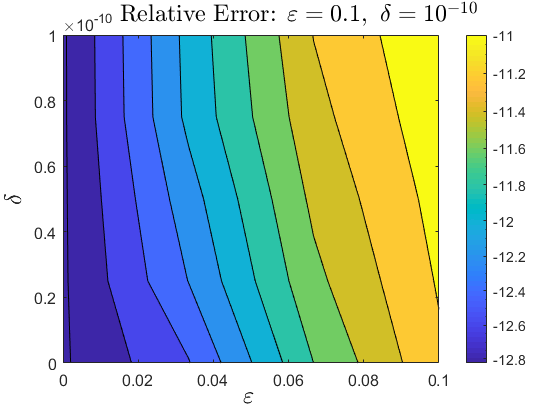
\includegraphics[width=7.6cm]{sections/7_conclusions_and_future_directions/Large_Eps_Small_Delta_2.png} }}%
    %\qquad
    \subfloat[\centering Small $\varepsilon$, Large $\delta$ ]{{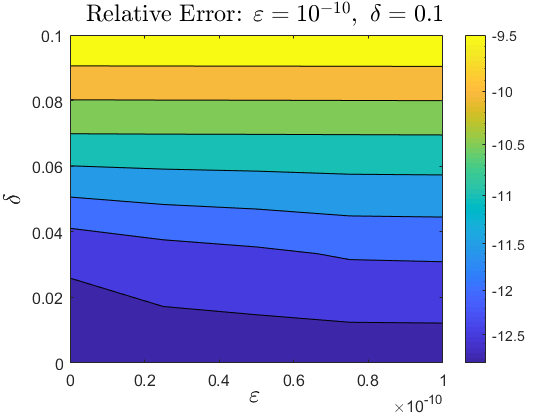
\includegraphics[width=7.6cm]{sections/7_conclusions_and_future_directions/Small_Eps_Large_Delta_2.png} }}%
    \vspace{3 mm}
    \caption{A contour plot of the relative error computed with our HOPS/AWE algorithm by holding $N=M=8$ Taylor orders fixed. In Figure $34\text{(a)}$ we expand up to $\Eps = 0.1$ and $\delta = 10^{-10}$ simultaneously with $N=M=8$ Taylor orders. In Figure $34\text{(b)}$ we expand up to $\Eps = 10^{-10}$ and $\delta = 0.1$ simultaneously with $N=M=8$ Taylor orders.}%
    \label{fig:example}%
\end{figure}
\vspace{-18mm}
Supplementary testing in both the upper and lower layers confirms that our HOPS/AWE algorithm is better suited towards larger $\varepsilon$.
%\begin{flushleft}
\newline
\\
\textbf{Predictions:} Our HOPS/AWE methodology takes advantage of exact enforcement of the \gls{owc} at an artificial boundary in order to truncate the computational domain to one of finite extent. After flattening the surface, the DNOs recover information through the solution stored at the interface. We suspect that this process mitigates large perturbations of the height/slope. By following techniques developed in \cite{NichollsReitich00b,NichollsTaber06,Nicholls16b,NichollsShen08}, we intend to rigorously prove that the TFE method is analytic when $\varepsilon$ is large. Additionally, we are interested in perturbing other physical parameters in the context of layered media problems. These are discussed in the engineering literature \cite{mashayekh2018parameter,mashayekh2018parameter2}.
\section{Rayleigh Singularities}
\label{Sec: Rayleigh Singularities}
A fundamental equation in the HOPS/AWE algorithm is
$$\alpha_p^2 + (\gamma_p^q(\delta))^2 = (k^q)^2,$$
where $k^q$ represents the wavenumber, $q\in\{u,w\}$, and $\alpha=k^q\sin(\theta), \gamma=k^q\cos(\theta),$ are parameters corresponding to refraction/reflection of the incidence angle $\theta$. As shown in $\S 5.4$, a Rayleigh singularity (or Wood's anomaly) occurs when $\ualpha_p^2 = (\uk^q)^2$ for any integer $p\neq 0$. That is, if $\ugamma_p^q(\delta) =0$ for $p\neq 0$ then the Taylor series expansion of $\gamma_p^q(\delta)$ is invalid. In \cite{Nicholls16}, the author investigated changing the Taylor expansion to a Puiseux expansion \cite{basu2007algorithms}:
$$\gamma_p^q(\delta)=\sum_{m=0}^{\infty}\gamma_{p,m}^q\delta^{m+1/2}=\delta^{1/2}\sum_{m=0}^{\infty}\gamma_{p,m}^q\delta^m.$$
However, he found that this approach ran into external difficulties ($\S$6 of \cite{Nicholls16}) simplifying explicit forms of the Dirichlet and Neumann trace operators.
\newline
\\
\textbf{Predictions:} Rayleigh singularities are a central obstruction to the convergence of our HOPS/AWE algorithm. In all of our numerical tests, we select custom frequency ranges which maximize the radius of convergence of our algorithm by expanding away from the singularities (cf. $\S 5.6$). Alternative methods such as Padé summation also fail to be analytic in a neighborhood of a Rayleigh singularity. General perturbation theory provides a variety of known techniques \cite{suslov2005divergent,convfromdiv,Heinz2020,dienes1957taylor,arteca1984summation} for expanding around divergent perturbation series. We suspect that adding these techniques to our HOPS/AWE algorithm will allow us perform a series expansion of $\ugamma_p^q(\delta)$ that does not diverge when $\ugamma_p^q(\delta)=0.$
\section{Multiple Layers}
\label{Sec: Multiple Layers}

In \cite{Nicholls16b}, the author discusses how to apply our HOPS methodology in multilayered configurations. He considers a multilayered material with $M$ (finite) interfaces at 
$$z=a^{(m)}+g^{(m)}(x,y),\quad 1\leq m \leq M,$$
which are $d_x \times d_y$ periodic
$$g^{(m)}(x+d_x,y+d_y)=g^{(m)}(x,y),\quad 1\leq m \leq M,$$
separating $(M+1)$--many layers.
%\vspace{-12mm}
\begin{figure}[H]
    \centering
    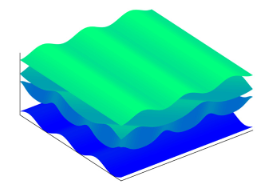
\includegraphics[width=7.6cm]{sections/7_conclusions_and_future_directions/multilayered.png}%
    \vspace{3mm}
    \caption{A five--layer problem configuration with layer interfaces $z = a^{(m)}+g^{(m)}(x).$}%
    \label{fig:example}%
\end{figure}
\vspace{-15mm}
%\begin{flushleft}
A generalization of our analyticity theorems (cf. $\S 4.5$) up to $M$ parameters is included as Theorem~$3.2$ in \cite{Nicholls16b}. For this, we consider quite general systems of linear equations of the form
%\end{flushleft}
\be
\bA(\tEps)\bV(\tEps)=\bR(\tEps),
\ee
where 
\bes
\bA(\tEps)=\sum_{\tn=0}^{\infty}\bA_{\tn}\tEps^{\tn},\quad 
\bR(\tEps) = \sum_{\tn=0}^{\infty}\bR_{\tn}\tEps^{\tn}.
\ees
The tildes represent multi--index notation \cite{Evans10}, in particular
\bes
\tEps := \begin{pmatrix} \Eps_1 \\ \vdots \\ \Eps_M \end{pmatrix},
\quad
\tn := \begin{pmatrix} n_1 \\ \vdots \\ n_M \end{pmatrix},
\ees
and the convention
\bes
\sum_{\tn=0}^{\infty} 
    A_{\tn}\ \tEps^{\tn}
  = \sum_{n_1=0}^{\infty} \cdots \sum_{n_M=0}^{\infty}
    A_{n_1,\ldots,n_M} \Eps_1^{n_1} \cdots \Eps_M^{n_M}.
\ees
As in $\S 4.5$, we seek a solution of the form
\be
\bV(\tEps)=\sum_{\tn=0}^{\infty}\bV_{\tn}\tEps^{\tn},
\ee
and from $(7.1)$ we find at order $\mathcal{O}(\tEps^{\tn})$
\bes
\bA_0\bV_{\tn}= \bR_{\tn} - \left(\sum_{\tl=0}^{\tn}\bA_{\tn-\tl}\bV_{\tl}- \bA_0\bV_{\tn}\right),
\ees
or
\be
\bV_{\tn}= \bA_0^{-1}\left\{\bR_{\tn} - \left(\sum_{\tl=0}^{\tn}\bA_{\tn-\tl}\bV_{\tl}- \bA_0\bV_{\tn}\right)\right\}.
\ee
The above notation represents multi--indices in the form
\bes
\sum_{\tl=0}^{\tn}\bA_{\tn-\tl}\bV_{\tl} = \sum_{\ell_1=0}^{n_1}\cdots \sum_{\ell_M=0}^{n_M}
    \bA_{n_1-\ell_1,\ldots,n_M-\ell_M} \bV_{\ell_1,\ldots,\ell_m},  
\ees
where $\tn=(n_1,\ldots,n_M),$ $\tl=(\ell_1,\ldots,\ell_M),$ and $0=(0,\ldots,0)$ with the convention
\bes
\tn \geq 0 \iff n_1\geq 0,\ldots,n_M\geq 0, \quad\tl \geq 0 \iff \ell_1\geq 0,\ldots,\ell_M\geq 0.
\ees
With these, we can extend our existence theorem (Theorem $4.5.1$) to $M$ parameters.
\begin{theorem}
\label{Thm:AVR}
Given two Banach spaces, $X$ and $Y$, suppose that:
\begin{enumerate}[label={\upshape[\arabic*]}]
\item $\bR_{\tn} \in Y$ for all $\tn \geq 0$,
  and there exist $M$--multi--indexed constants $C_R > 0$, $B_R > 0$,
  \bes
  C_R = \begin{pmatrix} C_{R,1} \\ \vdots \\ C_{R,M} \end{pmatrix},
  \quad
  B_R^{\tn} = \begin{pmatrix} B_{R,1}^{n_1} \\ \vdots \\ 
  B_{R,M}^{n_M} \end{pmatrix},
  \ees
  such that
  \bes
  \Norm{\bR_{\tn}}{Y} \leq C_R B_R^{\tn},
  \ees
\item $\bA_{\tn}: X \rightarrow Y$ for all
  $\tn \geq 0$, and there exist $M$--multi--indexed
  constants $C_A > 0$, $B_A > 0$ such that
  \bes
  \Norm{\bA_{\tn}}{X \rightarrow Y} \leq C_A B_A^{\tn},
  \ees
\item $\bA_0^{-1}: Y \rightarrow X$, and there 
  exists a constant $C_e > 0$ such that
  \bes
  \Norm{\bA_0^{-1}}{Y \rightarrow X} \leq C_e.
  \ees  
\end{enumerate}
Then the equation $(7.1)$ has a unique solution,
\be
\label{Eqn:V:Exp:Multi}
\bV(\tEps) = \sum_{\tn=0}^{\infty} \bV_{\tn} \tEps^{\tn},
\ee
and there exist $M$--multi--indexed constants $C_V > 0$ and $B_V > 0$ such that
\bes
\Norm{\bV_{\tn}}{X} \leq C_V B_V^{\tn},
\ees
for all $\tn \geq 0$ and any
\bes
C_V \geq 2 C_e C_R,
\quad
B_V \geq \max \left\{ B_R, 2 B_A, 2^{M+1} C_e C_A B_A \right\},
\ees
enforced componentwise. This implies that, for any $M$--multi--indexed constant
$0 \leq \tilde{\rho} < 1$, 
$(7.4)$, converges for all $\tEps$ such that
$B \tEps < \tilde{\rho}$, i.e., $\tEps < \tilde{\rho}/B$.
\end{theorem}
\begin{remark}
Our proof strategy is a form of multidimensional induction where given a statement $\bP(n_1, n_2, n_3, ..., n_M)$ for some $M\in \mathbb{N}$, we will show that $\forall n_1, n_2,\ldots, n_M \geq 0$, $\bP(n_1, n_2, n_3, ..., n_M)$ is true by inducting on $n_M$. We will follow the steps outlined below.
\begin{enumerate}
\item Establish $\bP(0,\ldots,n_j,\ldots,0)$ for all $1 \leq j < M$ and $n_1,\ldots,n_j \geq 0.$
\item Given $\bP(n_1,n_2,\ldots,n_j,\ldots,0)$ for all $1 \leq j < M$ and $n_1,\ldots,n_j \geq 0$, establish $\bP(n_1,n_2,\ldots,\bar{n}_j,\ldots,0)$. This can be accomplished through the two steps below.
\begin{enumerate}
    \item Establish $\bP(0,\ldots,\bar{n}_j,\ldots,0)$ for all $\bar{n}_j \geq 0$ (where the hypothesis in $[2]$ gives the required case for $n_j < \bar{n}_j$).
    \item Given  $\bP(n_1,n_2,\ldots,\bar{n}_j,\ldots,0)$ for all $1 \leq j < M$ and $n_1 < \bar{n}_1,  n_2 < \bar{n}_2,\ldots, $ $n_{j-1}  < \bar{n}_{j-1}$ and $\bar{n}_j\geq 0$, establish $\bP(\bar{n}_1,\bar{n}_2,\ldots,\bar{n}_j,\ldots,0)$.
\end{enumerate}
\item Given $\bP(n_1,n_2,\ldots,n_j,n_{j+1},\ldots,0)$ for all $1 \leq j+1 < M$ and $n_1,\ldots,n_{j+1} \geq 0$, establish $\bP(n_1,n_2,\ldots,n_j,\bar{n}_{j+1},\ldots,0)$. This can be accomplished by following the two steps outlined below. 
\begin{enumerate}
    \item Establish $\bP(0,\ldots,\bar{n}_{j+1},\ldots,0)$ for all $\bar{n}_{j+1} \geq 0$ (where the hypothesis in $[3]$ gives the required case for $n_{j+1} < \bar{n}_{j+1}$).
    \item Given  $\bP(n_1,n_2,\ldots,n_j,\bar{n}_{j+1},\ldots,0)$ for all $1 \leq j+1 < M$ and  $n_1 < \bar{n}_1,  n_2 < \bar{n}_2,\ldots, n_{j} < \bar{n}_{j}$ and $\bar{n}_{j+1}\geq 0$, establish $\bP(\bar{n}_1,\bar{n}_2,\ldots,\bar{n}_j,\bar{n}_{j+1}\ldots,0)$.
\end{enumerate}
\item Given $\bP(n_1,n_2,\ldots,n_{M-1},n_M)$ for all $n_1,n_2,\ldots,n_{M-1} \geq 0$ and $n_M < \bar{n}_M$, establish $\bP(n_1,n_2,\ldots,n_{M-1},\bar{n}_M)$. This can be accomplished by the two steps below (the base cases are handled through $[2]$ and $[3]$).
\begin{enumerate}
    \item Establish $\bP(0,\ldots,\bar{n}_{M})$ for $\bar{n}_{M} \geq 0$ (where the hypothesis in $[4]$ handles the required case for  $n_{M} < \bar{n}_{M}$).
    \item Given $\bP(n_1,n_2,\ldots,n_{M-1},\bar{n}_M)$ for all $n_1 < \bar{n}_1, n_2 < \bar{n}_2, \ldots n_{M-1} < \bar{n}_{M-1}$ and $\bar{n}_M \geq 0$, establish $\bP(\bar{n}_1,\bar{n}_2,\ldots,\bar{n}_{M-1},\bar{n}_M)$.
\end{enumerate}
\end{enumerate}

\end{remark}

\begin{proof}{[Theorem 7.4.1]} As with $\tEps$ and $\tn$, we represent $\tilde{\rho}$ by
\bes
\tilde{\rho} := \begin{pmatrix} \rho_1 \\ \vdots \\ \rho_M \end{pmatrix}.
\ees
As before, we will work by induction and consider the general case for finite $M>0$ where we want to establish
\bes
\norm{\bV_{n_1,\ldots,n_M}}_X \leq C_{V,1}\ldots C_{V,M} B_{V,1}^{n_1}\ldots B_{V,M}^{n_M}, \quad \forall n_1,\ldots,n_M\geq 0.
\ees
We prove this via an induction on $n_M$. The base case $n_1,n_2,\ldots, n_{j-1},n_{j+1},\ldots,$ $n_M=0$ and $1 \leq j < M$:
\bes
\norm{\bV_{0,\ldots,n_j,\ldots,0}}_X \leq C_{V,j} B_{V,j}^{n_j}, \quad \forall n_j\geq 0,
\ees
has previously been established by Theorem $4.5.1$ where $\tEps = \Eps_j$ and $\delta=0$. We now assume
\bes
\norm{\bV_{n_1,\ldots,n_j,\ldots,0}}_X \leq  C_{V,1}\ldots C_{V,j}B_{V,1}^{n_1}\ldots B_{V,j}^{n_j}, ~~ \forall n_1,\ldots,n_{j-1}\geq 0,~~ \forall n_j < \bar{n}_j,~~ 1 \leq j < M,
\ees
and seek
\bes
\norm{\bV_{n_1,\ldots,\bar{n}_j,\ldots,0}}_X \leq  C_{V,1}\ldots C_{V,j}B_{V,1}^{n_1}\ldots B_{V,j}^{\bar{n}_j}, ~~ \forall n_1,\ldots,n_{j-1}\geq 0.
\ees
This can be obtained through a chain of $(M-1)$ inductions on $n_1,\ldots,n_j$ where $1 \leq j < M$. For simplicity, we will show what happens in the arbitrary case $n_j$. The base case $n_1,\ldots,n_{j-1}=0$:
\bes
\norm{\bV_{0,\ldots,\bar{n}_j,\ldots,0}}_X \leq  C_{V,j}B_{V,j}^{\bar{n}_j}, \quad \forall \bar{n}_j \geq 0,
\ees
is established by Theorem $4.5.1$ where $\tEps = \Eps_j$ and $\delta=0$. Therefore, we assume
\begin{align*}
\norm{\bV_{n_1,\ldots,\bar{n}_j,\ldots,0}}_X \leq  C_{V,1}\ldots C_{V,j}B_{V,1}^{n_1}\ldots B_{V,j}^{\bar{n}_j},~~\forall n_1  &< \bar{n}_1,\ldots, n_{j-1} < \bar{n}_{j-1},~~ \forall \bar{n}_j \geq 0,\\&~ 1 \leq j < M,
\end{align*}
and seek
\bes
\norm{\bV_{\bar{n}_1,\ldots,\bar{n}_j,\ldots,0}}_X \leq  C_{V,1}\ldots C_{V,j}B_{V,1}^{\bar{n}_1}\ldots B_{V,j}^{\bar{n}_j}.
\ees
Recalling $\tn=(n_1,\ldots,n_j)$ and  $\tl=(\ell_1,\ldots,\ell_j)$, we define
\be
{\sum_{\tl=0}^{\tn}}^{*}\bA_{\tn-\tl}\bV_{\tl} := \sum_{\tl=0}^{\tn}\bA_{\tn-\tl}\bV_{\tl} - \bA_0\bV_{\tn},
\ee
and apply $(7.3),(7.5)$ and the mapping properties of $\bA_{0}^{-1}$ to find
\bes
\norm{\bV_{\bar{n}_1,\ldots,\bar{n}_j,\ldots,0}}_X\leq C_e\left\{\norm{\bR_{\bar{n}_1,\ldots,\bar{n}_j}}_Y + {\sum_{\tl=0}^{\tn}}^{*}\norm{\bA_{\tn-\tl}\bV_{\tl}}_Y\right\}.
\ees
Using the estimates on $\bR_{n_1,\ldots,n_j}$ and $\bA_{n_1,\ldots,n_j}$ (for all $n_1,\ldots,n_j$) and $\bV_{n_1,\ldots,n_j}$ $(n_1 < \bar{n}_1, \ldots, n_j < \bar{n}_j)$ we have
\begin{align*}
\norm{\bV_{\bar{n}_1,\ldots,\bar{n}_j,\ldots,0}}_X &\leq
C_e\Bigg\{C_{R,1}\ldots C_{R,j}B_{R,1}^{\bar{n}_1}\ldots B_{R,j}^{\bar{n}_j} + {\sum_{\tl=0}^{\tn}}^{*}C_{A,1}\ldots C_{A,j}B_{A,1}^{\bar{n}_1-\ell_1}\ldots B_{A,j}^{\bar{n}_j-\ell_j}\\ & \qquad \qquad \qquad \qquad \qquad \qquad \qquad \qquad \times
C_{V,1}\ldots C_{V,j}B_{V,1}^{\ell_1}\ldots B_{V,j}^{\ell_j}\Bigg\} \\& =
C_eC_{R,1}\ldots C_{R,j}B_{R,1}^{\bar{n}_1}\ldots B_{R,j}^{\bar{n}_j} + C_eC_{A,1}\ldots C_{A,j}C_{V,1}\ldots C_{V,j} \\&
~~ \times \left(\frac{B_{A,1}}{B_{V,1}}\right)B_{V,1}^{\bar{n}_1}\cdots \left(\frac{B_{A,j}}{B_{V,j}}\right)B_{V,j}^{\bar{n}_j}{\sum_{\tl=0}^{\tn}}^{*}
\left(\frac{B_{A,1}}{B_{V,1}}\right)B_{V,1}^{\bar{n}_1-\ell_1-1}\cdots \\& ~~ \times
\left(\frac{B_{A,j}}{B_{V,j}}\right)B_{V,j}^{\bar{n}_j-\ell_j-1} \\& \leq
C_eC_{R,1}\ldots C_{R,j}B_{V,1}^{\bar{n}_1}\ldots B_{V,j}^{\bar{n}_j} + C_eC_{A,1}\ldots C_{A,j}C_{V,1}\ldots C_{V,j} \\& ~~ \times
\left(\frac{B_{A,1}}{B_{V,1}}\right)B_{V,1}^{\bar{n}_1}\cdots\left(\frac{B_{A,j}}{B_{V,j}}\right)B_{V,j}^{\bar{n}_j}\left(\frac{1}{1-1/2}\right)^j,
\end{align*}
if $B_{A,k}/B_{V,k} \leq 1/2$, $k=1,\ldots,j$ (implying $B_{V,k} \geq 2B_{A,k}$). We are done if we demand that
\bes
B_{V,k} \geq B_{R,k}, \quad C_eC_{R,k} \leq C_{V,k}/2, \quad 2^jC_eC_{A,k}C_{V,k}(B_{A,k}/B_{V,k}) \leq 
C_{V,k}/2.
\ees
This can be realized if
\bes
C_{V,k} \geq 2C_eC_{R,k}, \quad
B_{V,k} \geq \max\left\{B_{R,k},2B_{A,k},2^{j+1}C_eC_{A,k}B_{A,k}\right\}.
\ees
We then assume
\begin{align*}
\norm{\bV_{n_1,\ldots,n_{j+1},\ldots,0}}_X \leq  C_{V,1}\ldots C_{V,j+1}B_{V,1}^{n_1}\ldots B_{V,j+1}^{n_{j+1}}, ~~ &\forall n_1,\ldots,n_j\geq 0,~~ \forall n_{j+1} < \bar{n}_{j+1},\\&~~ 1 \leq j < M,
\end{align*}
and seek
\bes
\norm{\bV_{n_1,\ldots,\bar{n}_{j+1},\ldots,0}}_X \leq  C_{V,1}\ldots C_{V,j+1}B_{V,1}^{n_1}\ldots B_{V,j+1}^{\bar{n}_{j+1}}, ~~ \forall n_1,\ldots,n_{j}\geq 0.
\ees
As before, this can be obtained through a chain of $M$ inductions on $n_1,\ldots,n_{j+1}$ where $1 \leq j < M$. For simplicity, we will show what happens in the arbitrary case $n_{j+1}$. The base case $n_1,\ldots,n_{j}=0$:
\bes
\norm{\bV_{0,\ldots,\bar{n}_{j+1},\ldots,0}}_X \leq  C_{V,j+1}B_{V,j+1}^{\bar{n}_{j+1}}, \quad \forall \bar{n}_{j+1} \geq 0,
\ees
is established by Theorem $4.5.1$ where $\tEps = \Eps_{j+1}$ and $\delta=0$. Therefore, we assume
\begin{align*}
\norm{\bV_{n_1,\ldots,\bar{n}_{j+1},\ldots,0}}_X \leq  C_{V,1}\ldots C_{V,j+1}B_{V,1}^{n_1}\ldots B_{V,j+1}^{\bar{n}_{j+1}},~~\forall n_1  &< \bar{n}_1,\ldots, n_{j} < \bar{n}_{j},~~ \forall \bar{n}_{j+1} \geq 0,\\&~ 1 \leq j < M,
\end{align*}
and seek
\bes
\norm{\bV_{\bar{n}_1,\ldots,\bar{n}_{j+1},\ldots,0}}_X \leq  C_{V,1}\ldots C_{V,j+1}B_{V,1}^{\bar{n}_1}\ldots B_{V,j+1}^{\bar{n}_{j+1}}.
\ees
In this scenario, $\tn=(n_1,\ldots,n_{j+1})$ and  $\tl=(\ell_1,\ldots,\ell_{j+1}),$ so we apply $(7.3),(7.5)$ and the mapping properties of $\bA_{0}^{-1}$ to find
\bes
\norm{\bV_{\bar{n}_1,\ldots,\bar{n}_{j+1},\ldots,0}}_X\leq C_e\left\{\norm{\bR_{\bar{n}_1,\ldots,\bar{n}_{j+1}}}_Y + {\sum_{\tl=0}^{\tn}}^{*}\norm{\bA_{\tn-\tl}\bV_{\tl}}_Y\right\}.
\ees
Using the estimates on $\bR_{n_1,\ldots,n_{j+1}}$ and $\bA_{n_1,\ldots,n_{j+1}}$ (for all $n_1,\ldots,n_{j+1}$) and $\bV_{n_1,\ldots,n_{j+1}}$ $(n_1 < \bar{n}_1, \ldots, n_{j+1} < \bar{n}_{j+1})$ we have
\begin{align*}
\norm{\bV_{\bar{n}_1,\ldots,\bar{n}_{j+1},\ldots,0}}_X &\leq
C_e\Bigg\{C_{R,1}\ldots C_{R,{j+1}}B_{R,1}^{\bar{n}_1}\ldots B_{R,{j+1}}^{\bar{n}_{j+1}} + {\sum_{\tl=0}^{\tn}}^{*}C_{A,1}\ldots C_{A,{j+1}}B_{A,1}^{\bar{n}_1-\ell_1}\ldots \\ & \qquad \qquad \qquad \qquad \qquad \quad \times
B_{A,{j+1}}^{\bar{n}_{j+1}-\ell_{j+1}}C_{V,1}\ldots C_{V,{j+1}}B_{V,1}^{\ell_1}\ldots B_{V,{j+1}}^{\ell_{j+1}}\Bigg\} \\& =
C_eC_{R,1}\ldots C_{R,{j+1}}B_{R,1}^{\bar{n}_1}\ldots B_{R,{j+1}}^{\bar{n}_{j+1}} + C_eC_{A,1}\ldots C_{A,{j+1}}C_{V,1}\ldots C_{V,{j+1}} \\&
~~ \times \left(\frac{B_{A,1}}{B_{V,1}}\right)B_{V,1}^{\bar{n}_1}\cdots \left(\frac{B_{A,{j+1}}}{B_{V,{j+1}}}\right)B_{V,{j+1}}^{\bar{n}_{j+1}}{\sum_{\tl=0}^{\tn}}^{*}
\left(\frac{B_{A,1}}{B_{V,1}}\right)B_{V,1}^{\bar{n}_1-\ell_1-1}\cdots \\& ~~ \times
\left(\frac{B_{A,{j+1}}}{B_{V,{j+1}}}\right)B_{V,{j+1}}^{\bar{n}_{j+1}-\ell_{j+1}-1} \allowdisplaybreaks\\& \leq
C_eC_{R,1}\ldots C_{R,{j+1}}B_{V,1}^{\bar{n}_1}\ldots B_{V,{j+1}}^{\bar{n}_{j+1}} + C_eC_{A,1}\ldots C_{A,{j+1}}C_{V,1}\ldots C_{V,{j+1}} \\& ~~ \times
\left(\frac{B_{A,1}}{B_{V,1}}\right)B_{V,1}^{\bar{n}_1}\cdots\left(\frac{B_{A,{j+1}}}{B_{V,{j+1}}}\right)B_{V,{j+1}}^{\bar{n}_{j+1}}\left(\frac{1}{1-1/2}\right)^{j+1},
\end{align*}
if $B_{A,t}/B_{V,t} \leq 1/2$, $t=1,\ldots,j+1$ (implying $B_{V,t} \geq 2B_{A,t}$). We are done if we demand that
\bes
B_{V,t} \geq B_{R,t}, \quad C_eC_{R,t} \leq C_{V,t}/2, \quad 2^{j+1}C_eC_{A,t}C_{V,t}(B_{A,t}/B_{V,t}) \leq 
C_{V,t}/2.
\ees
This can be realized if
\bes
C_{V,t} \geq 2C_eC_{R,t}, \quad
B_{V,t} \geq \max\left\{B_{R,t},2B_{A,t},2^{j+2}C_eC_{A,t}B_{A,t}\right\}.
\ees
To complete the general case for finite $M>0$, we assume
\bes
\norm{\bV_{n_1,\ldots,n_M}}_X \leq  C_{V,1}\ldots C_{V,M}B_{V,1}^{n_1}\ldots B_{V,M}^{n_M}, ~~ \forall n_1,\ldots,n_{M-1}\geq 0,~~ \forall n_M < \bar{n}_M,
\ees
and seek
\bes
\norm{\bV_{n_1,\ldots,\bar{n}_M}}_X \leq  C_{V,1}\ldots C_{V,M}B_{V,1}^{n_1}\ldots B_{V,M}^{\bar{n}_M}, ~~ \forall n_1,\ldots,n_{M-1}\geq 0.
\ees
The base case $n_1,n_2,\ldots,n_{M-1}=0$:
\bes
\norm{\bV_{0,\ldots,\bar{n}_M}}_X \leq  C_{V,M}B_{V,M}^{\bar{n}_M}, \quad \forall \bar{n}_M \geq 0,
\ees
has previously been established by Theorem $4.5.1$ where $\tEps = \Eps_M$ and $\delta =0$. Finally, we assume
\begin{align*}
\norm{\bV_{n_1,\ldots,n_{M-1},\bar{n}_M}}_X \leq  C_{V,1}\ldots C_{V,M}B_{V,1}^{n_1}\ldots B_{V,M}^{\bar{n}_M},~~~&\forall n_1  < \bar{n}_1,\ldots, n_{M-1} < \bar{n}_{M-1},\\&~~~~ \forall \bar{n}_M \geq 0,
\end{align*}
and seek
\bes
\norm{\bV_{\bar{n}_1,\ldots,\bar{n}_{M-1},\bar{n}_M}}_X \leq  C_{V,1}\ldots C_{V,M}B_{V,1}^{\bar{n}_1}\ldots B_{V,M}^{\bar{n}_M}.
\ees
In this case, $\tn=(n_1,\ldots,n_M)$ and  $\tl=(\ell_1,\ldots,\ell_M),$ so we apply $(7.3),(7.5)$ and the mapping properties of $\bA_{0}^{-1}$ to find
\bes
\norm{\bV_{\bar{n}_1,\ldots,\bar{n}_M}}_X\leq C_e\left\{\norm{\bR_{\bar{n}_1,\ldots,\bar{n}_M}}_Y + {\sum_{\tl=0}^{\tn}}^{*}\norm{\bA_{\tn-\tl}\bV_{\tl}}_Y\right\}.
\ees
Using the estimates on $\bR_{n_1,\ldots,n_M}$ and $\bA_{n_1,\ldots,n_M}$ (for all $n_1,\ldots,n_M$) and $\bV_{n_1,\ldots,n_M}$ $(n_1 < \bar{n}_1, \ldots, n_M < \bar{n}_M)$ we have
\vspace{-1.5mm}
\begin{align*}
\norm{\bV_{\bar{n}_1,\ldots,\bar{n}_M}}_X &\leq
C_e\Bigg\{C_{R,1}\ldots C_{R,M}B_{R,1}^{\bar{n}_1}\ldots B_{R,M}^{\bar{n}_M} + {\sum_{\tl=0}^{\tn}}^{*}C_{A,1}\ldots C_{A,M}B_{A,1}^{\bar{n}_1-\ell_1}\ldots B_{A,M}^{\bar{n}_M-\ell_M}\\ & \qquad \qquad \qquad \qquad \qquad \qquad \qquad \qquad \times
C_{V,1}\ldots C_{V,M}B_{V,1}^{\ell_1}\ldots B_{V,M}^{\ell_M}\Bigg\} \\& =
C_eC_{R,1}\ldots C_{R,M}B_{R,1}^{\bar{n}_1}\ldots B_{R,M}^{\bar{n}_M} + C_eC_{A,1}\ldots C_{A,M}C_{V,1}\ldots C_{V,M} \\& 
~~ \times \left(\frac{B_{A,1}}{B_{V,1}}\right)B_{V,1}^{\bar{n}_1}\cdots \left(\frac{B_{A,M}}{B_{V,M}}\right)B_{V,M}^{\bar{n}_M}{\sum_{\tl=0}^{\tn}}^{*}
\left(\frac{B_{A,1}}{B_{V,1}}\right)B_{V,1}^{\bar{n}_1-\ell_1-1}\cdots \\& \allowdisplaybreaks~~ \times
\left(\frac{B_{A,M}}{B_{V,M}}\right)B_{V,M}^{\bar{n}_M-\ell_M-1} \\&  \leq
C_eC_{R,1}\ldots C_{R,M}B_{V,1}^{\bar{n}_1}\ldots B_{V,M}^{\bar{n}_M} + C_eC_{A,1}\ldots C_{A,M}C_{V,1}\ldots C_{V,M} \\& ~~ \times
\left(\frac{B_{A,1}}{B_{V,1}}\right)B_{V,1}^{\bar{n}_1}\cdots\left(\frac{B_{A,M}}{B_{V,M}}\right)B_{V,M}^{\bar{n}_M}\left(\frac{1}{1-1/2}\right)^M,
\end{align*}
if $B_{A,i}/B_{V,i} \leq 1/2$, $i=1,\ldots,M$ (implying $B_{V,i} \geq 2B_{A,i}$). We are done if we demand that
\bes
B_{V,i} \geq B_{R,i}, \quad C_eC_{R,i} \leq C_{V,i}/2, \quad 2^MC_eC_{A,i}C_{V,i}(B_{A,i}/B_{V,i}) \leq 
C_{V,i}/2.
\ees
This can be realized if
\bes
C_{V,i} \geq 2C_eC_{R,i}, \quad
B_{V,i} \geq \max\left\{B_{R,i},2B_{A,i},2^{M+1}C_eC_{A,i}B_{A,i}\right\}.
\ees
\end{proof}
Using a similar approach in conjunction with the analysis in Chapters $2$ and $3$, we predict a more general form of Theorems $2.9.2$ and $3.8.1$ exists, which would establish the analyticity of the transformed field with respect to any finite $M > 0$ perturbation parameters.
\vspace{1mm}
\begin{conjecture} 
\label{Conj:u,w:Anal:n:n_m}
Given any integer $s \geq 0$, if $f \in C^{s+2}([0,d])$ and 
$U_{\tilde{n}} \in H^{s+3/2}([0,d])$, $W_{\tilde{n}}\in H^{s+3/2}([0,d])$ such that
\bes
\|U_{\tilde{n}}\|_{H^{s+3/2}} \le K_U B_U^{\tn} , \quad
\|W_{\tilde{n}}\|_{H^{s+3/2}} \le K_W B_W^{\tn} ,
\ees
for constants $K_U, K_W>0$ and $M$--multi--indexed constants $B_U, B_W > 0$, then 
$u_{\tn} \in H^{s+2}([0,d]\times[0,a])$, $w_{\tn}\in H^{s+2}([0,d]\times[-b,0])$ and
\bes
\label{Eqn:u,w:Est:n:n_m}
\|u_{\tn}\|_{H^{s+2}} \le K B^{\tn}, \quad
\|w_{\tn}\|_{H^{s+2}} \le \tilde{K}\tilde{B}^{\tn} ,
\ees
for constants $K,\tilde{K}> 0$ and $M$--multi--indexed constants $B ,\tilde{B}>0$.
\end{conjecture}
\vspace{1mm}
Analogously, a similar procedure would establish a more general form of Theorems $2.10.2$ and $3.9.2$ for the analyticity of the DNOs for any finite $M>0$ perturbation parameters.
\vspace{1mm}
\begin{conjecture} 
\label{Thm:G,J:Anal:n:n_m}
Given any integer $s \geq 0$, if $f \in C^{s+2}([0,d])$ and 
$U_{\tn} \in H^{s+3/2}([0,d])$, $W_{\tn} \in H^{s+3/2}([0,d])$ such that
\bes
\SobNorm{U_{\tn}}{s+3/2} \leq K_U B_U^{\tn}, \quad
\SobNorm{W_{\tn}}{s+3/2} \leq K_W B_W^{\tn},
\ees
for constants $K_U,K_W> 0$ and $M$--multi--indexed constants $B_U, B_W > 0$, then $G_{\tn} \in H^{s+1/2}([0,d])$, $J_{\tn} \in H^{s+1/2}([0,d])$ and
\bes
\label{Eqn:G,J:Est:n:n_m} 
\|G_{\tn}\|_{H^{s+1/2}} \le \tilde{K}\tilde{B}^{\tn}, \quad
\|J_{\tn}\|_{H^{s+1/2}} \le \dbtilde{K} \dbtilde{B}^{\tn},
\ees
for constants $\tilde{K},\dbtilde{K}  > 0$ and $M$--multi--indexed constants $\tilde{B},\dbtilde{B}>0$.
\end{conjecture}
\vspace{1mm}
Upon proving these, one has two key ingredients to the more general version of Theorem $4.6.1$ which establishes the existence and uniqueness of solutions to a system of partial differential equations with respect to $M$ perturbation parameters.
\vspace{1mm}
\begin{conjecture} 
\label{Conj:Main}
Given an integer $s \geq 0$, if $f \in C^{s+2}([0,d])$ then the 
equation $(7.1)$ has a unique solution, $(7.4)$,
and there exist a constant $C > 0$ and $M$--multi--indexed constants $B>0$ such that
\bes
\Norm{\bV_{\tn}}{X^s} \leq C B^{\tn},
\ees
for all $\tn \geq 0$.  This implies that for any $M$--multi--indexed constant
$0 \leq \tilde{\rho} < 1$, $(7.4)$, converges for all $\tEps$ such that
$B \tEps < \tilde{\rho}$, i.e., $\tEps < \tilde{\rho}/B$.
\end{conjecture}
\vspace{1mm}
\textbf{Predictions:} In application oriented fields such as signal processing or sea ice modeling, practitioners work with  multiple frequencies \cite{qiu2005high,bosse1995model,zhao2009multi,blanchard2021high} at short or long wavelengths. Also, as depicted in Figure $35$, the grating surface could have $M$ different layers \cite{imperatore2017perturbation} with distinct values of $g_j(x)=\Eps f_j(x),~j=1,\ldots, M$. A proof of Conjecture $7.4.4$ would enable the freedom to enforce any number of perturbation parameters and obtain an analytic solution. Given the widespread availability of parallel computing resources coupled with additional perturbation parameters associated with elastic media, we believe that future research will force hundreds or even thousands of distinct perturbation parameters, all of which should yield an analytic solution.
\section{Parallel Programming}
\setcounter{section}{5}
\label{Sec: Parallel Programming}

In the case of multiple layered interfaces, we need to compute intermediate DNOs for up to $M$ layers. This will greatly increase the computational cost and execution time of our HOPS/AWE algorithm and we suspect that it will be necessary to introduce parallel programming techniques to offset the computational expense. In the context of the \gls{oe} method, preliminary work \cite{fang2015operator} has been completed in C\texttt{++} to parallelize the computation of Navier's equations \cite{BillinghamKing00,achenbach2012wave}. These techniques can be adapted to the TFE method through the choice of OpenMP \cite{chandra2001parallel}, MPI \cite{snir1998mpi}, or CUDA \cite{sanders2010cuda}.
\newline
\\
\textbf{Predictions:} In two or three dimensions, our HOPS code is robust, efficient and has a runtime less than an hour. A local machine with an Intel Core i$5$ CPU, $8$GB of RAM, and Windows $10$ OS completed almost every simulation in this thesis in less than thirty minutes. However, with ten to one hundred layer configurations, we suspect that many simulations will take on the order of weeks or even months. As a result, it will be necessary to parallelize our Matlab code in a compiled programming language such as C or  C\texttt{++}.

\section{Alternatives to DNOs}
\label{Sec: Alternatives to DNOs}
In Chapter $4$ we wrote our scattering problem as a linear system
\bes
\bA \bV = \bR,
\ees
where, upon expanding $\{\bA,\bV,\bR\}$ in both $\varepsilon$ and $\delta$, we arrived at the flat--interface solution $\bA_{0,0}\bV_{0,0}=\bR_{0,0}$
at order $\mathcal{O}(\varepsilon^0,\delta^0)$. We then saw it was necessary to invert
\bes
\bA_{0,0} = \begin{pmatrix}I & -I\\
-G_{0,0} & -\tau^2J_{0,0}\end{pmatrix}, 
\ees
which features the two DNOs, $G_{0,0}$ and $J_{0,0}$, in order to show the existence and uniqueness of solutions. A primary feature of all HOPS schemes is the inversion of a single, sparse operator $\bA_{0,0}$ through the use of DNOs. However, one may ponder if a different technique could produce a more competitive algorithm that is comparable to our HOPS/AWE algorithm (or even better). Is it absolutely necessary to pass in transformed field data in order to efficiently compute and recover internal information stored at the grating surface?
\\
\newline
\textbf{Predictions:} A primary advantage of our HOPS/AWE scheme is that for every perturbation order, it is only necessary to invert a single sparse operator corresponding to a flat--interface, order--zero approximation. There are a number of competing approaches in general perturbation theory within the context of layered media problems. In regards to electromagnetic wave scattering, Galerkin and boundary element methods are discussed in \cite{escapil2020helmholtz,silva2017quantifying,nakata1990boundary,elschner2012optimization,rathsfeld2006} and a high--order perturbation approach based on boundary integral equations in \cite{dolz2020higher}. High--order schemes for linear waves can be computed using level set methods \cite{sethian1999level} and fast marching methods, as well as other methods involving domain decomposition \cite{el2004comparing,benamou1997domain,larsson1999domain,gong2021convergence,perez2018domain,chan1994domain}. A holistic evaluation of these competing methods could potentially improve our HOPS/AWE algorithm if we found a faster method of inverting linear operators without the use of DNOs.
\section{Computational Complexity}
\label{Sec: Computational Complexity}

One of the fundamental reasons for developing our HOPS/AWE algorithm is its advantageous computational complexity for problems within its domain of applicability.
In comparison with other classical methods, our HOPS/AWE approach has several advantages for computing quantities such as the Reflectivity Map, $R=R(\varepsilon,\delta)$. To demonstrate this we begin
by fixing the problem of computing $R$ for $N_{\Eps}$ many values of 
$\Eps$ and $N_{\delta}$ many values of $\delta$.

In the case of computing the DNOs $G$ and $J$, we recall from $\S 2.11$ and $\S 3.10$ that our HOPS/AWE algorithm requires
$N_x \times N_z$ unknowns at every perturbation order, $(n,m)$, corresponding to
the $N_x$ equally--spaced gridpoints in the lateral direction and the $N_z + 1$ collocation points in the vertical dimension. In $\S 4.5$ we saw that we could write our scattering problem as $\bA(\Eps,\delta) \bV(\Eps,\delta) = \bR(\Eps,\delta)$ where
\bes
    \bA(\Eps,\delta)=\sumn \summ \bA_{n,m}\Eps^n\delta^m, \quad \bR(\Eps,\delta) = \sumn \summ \bR_{n,m}\Eps^{n}\delta^m,
\ees
and
\bes
\label{Eqn:Soln:Two_Param_Append}
\bV(\Eps,\delta) = \sumn \summ \bV_{n,m}\Eps^{n}\delta^m.
\ees
At order $\mathcal{O}(\Eps^n,\delta^m)$ this becomes
\begin{align}
\begin{split}
\bA_{0,0}\bV_{n,m}=&~\bR_{n,m}-\sum_{\ell=0}^{n-1}\bA_{n-\ell,0}\bV_{\ell,m}-\sum_{r=0}^{m-1}\bA_{0,m-r}\bV_{n,r}\\&
-\sum_{\ell=0}^{n-1}\sum_{r=0}^{m-1}\bA_{n-\ell,m-r}\bV_{\ell,r}.
\end{split}
\end{align}
A careful study of $(7.6)$
reveals that the computational complexity of forming the
right--hand side at order $(n,m)$ is
\bes
\BigOh{n m N_x \log(N_x) N_z \log(N_z)}.
\ees
Inverting the operator $\bA_{0,0}$ has complexity $\BigOh{N_x \log(N_x) N_z \log(N_z)}$
so the full cost of computing the $\bV_{n,m}$, 
$\{ 0 \leq n \leq N, 0 \leq m \leq M \}$, is
\bes
\BigOh{N^2 M^2 N_x \log(N_x) N_z \log(N_z)}.
\ees
Once these coefficients are recovered, the cost of summing the series in 
$(\Eps,\delta)$ is minimal, provided it is done in an efficient manner 
(e.g., by Horner's rule \cite{BurdenFaires,AtkinsonHan01}). Our algorithm then 
requires an additional $\BigOh{N_{\Eps} N_{\delta}}$ steps to sum 
over every value of $(\Eps,\delta)$, therefore the full cost of 
computing the Reflectivity Map by our HOPS/AWE method is
\be
\BigOh{N^2 M^2 N_x \log(N_x) N_z \log(N_z) + N_{\Eps} N_{\delta}}.
\ee
In contrast, for a single $(\Eps,\delta)$ pair, a Boundary Integral Method solver with $N_x$ lateral
gridpoints requires time proportional to $\BigOh{N_x^3}$ for Gaussian elimination
to solve the resulting dense system of $N_x$ equations in $N_x$ unknowns
\cite{BurdenFaires,AtkinsonHan01,ColtonKress13}. Applying this 
$N_{\Eps} \times N_{\delta}$ times results in a total computational complexity of
\be
\BigOh{N_x^3 N_{\Eps} N_{\delta}}.
\ee
Thus, once $N_{\Eps}$ and $N_{\delta}$ become large, e.g.,

\bes
N_{\Eps} N_{\delta} > \frac{N^2 M^2 N_x \log(N_x) N_z \log(N_z)}{N_x^3},
\ees
our new algorithm becomes far more efficient. We speculate that the cost of $(7.7)$ could be reduced to
\be
\BigOh{N M \log(NM)N_x \log(N_x) N_z \log(N_z) + N_{\Eps} N_{\delta}},
\ee
provided that we develop a more efficient method of computing the $\bV_{n,m}$, 
$\{ 0 \leq n \leq N, 0 \leq m \leq M \}$, such as reducing the problem space at every step. Alternative approaches to layered media problems have also been proposed by other authors \cite{bai2004reduction,chew2005fast}, including interpolation \cite{atkins2010fast} and Green's function \cite{konno2016fast}.
\newline
\\
\textbf{Predictions:} The combination of implementing parallel programming techniques (through, e.g., OpenMP or CUDA) and reducing the problem space at every step will greatly enhance the speed and fidelity of our HOPS/AWE algorithm. Considering the natural advantage surface methods have over conventional methods, such as finite difference, finite element, and spectral element methods, we expect that our HOPS/AWE algorithm will be among the most competitive available for periodic layered media problems.
\chapter{Conclusions and Future Work}
\label{sec:conclusions_and_future_dir}

\fancyhead[LO]{\text{Chapter 7}\quad \text{Conclusions and Future Work}}

This thesis establishes a novel HOPS/AWE algorithm that is particularly well suited to simulating scattering returns for periodic media problems. Our main contribution is that of Theorem $4.6.1$ which guarantees the existence and uniqueness of solutions to a system of partial differential equations which model the interaction of linear waves in periodic layered structures with respect to multiple perturbation parameters. Through the introduction of DNOs and a change of variables based on the TFE methodology, we have shown that solutions to the Helmholtz problem are jointly analytic with respect to both interfacial and frequency perturbations. As a result, our HOPS/AWE algorithm is able to handle a variety of numerical simulations that are physically challenging in both the TE and TM polarization modes. Moreover, our extensive numerical results demonstrate the accuracy, speed, and robustness expected of all HOPS methods.


\section{Future Directions}
\label{Sec: Future Directions}
There are a wide range of improvements to both the HOPS/AWE algorithm and the proof of analyticity for linear waves in periodic layered media. Our main goals for future research are to expand the TFE method through a new proof of convergence, investigate expanding around singularities, evaluate analyticity theorems in multilayered configurations, add new parallel programming functionality, explore alternative methods to recover surface data without Dirichlet--Neumann Operators, and to reduce the execution time of the HOPS algorithm. We now summarize these six research goals and suggest predictions for future research.
\begin{enumerate}[labelsep=0ex,align=left,start=1]
    \item[\textbf{Goal 1-}] ~\textbf{Choice of Parameters: Does the geometry of the perturbation impact how large the size of the perturbation can be? }
    \item[\textbf{Goal 2-}] ~\textbf{Rayleigh Singularities: Can we build a full HOPS algorithm based on points where the Taylor expansion is invalid? }
    \item[\textbf{Goal 3-}] ~\textbf{Multiple Layers: Can we prove analyticity results when the number of layers is greater than three? Do the same theorems hold for ten or one hundred layers?} 
    \item[\textbf{Goal 4-}] ~\textbf{{Parallel Programming}: Can we implement parallel programming techniques so that our HOPS code runs on $N$ processors? }
    \item[\textbf{Goal 5-}] ~\textbf{{Alternatives to DNOs}: Do we need to use DNOs to recover surface data from information stored in the transformed field? Is there an alternative method which preserves the inversion of a single, sparse operator at the interface?   }
    \item[\textbf{Goal 6-}] ~\textbf{Computational Costs: Can we reduce the execution time per time step in our HOPS algorithm?} 
\end{enumerate}

\section{Choice of Parameters}
\label{Sec: Choice of Parameters}
Our HOPS/AWE algorithm is based on two smallness assumptions:
\begin{enumerate}
\item \text{Boundary Perturbation: $g(x)=\varepsilon f(x),$ $\varepsilon\in\mathbb R$, $\varepsilon \ll 1$,}
\vspace{-2mm}
\item \text{Frequency Perturbation: $\omega=(1+\delta)\underline{\omega}=\underline{\omega}+\delta\underline{\omega},$ $\omega\in\mathbb R$, $\delta \ll 1$,} 
\end{enumerate}
with the additional assumption that $f$ is sufficiently smooth ($f\in C^2$ \cite{NichollsReitich99,NichollsReitich03b} or even Lipschitz \cite{hu2005analyticity}). Numerical simulations show that our HOPS/AWE algorithm can handle larger perturbations of $\varepsilon$ (the height/slope) in comparison to $\delta$ (the frequency). With modest test parameters and a period of $d=2\pi$, we are able to perturb the value of $\varepsilon$ (to $\varepsilon=0.1$ or even $\varepsilon=0.2$) and still get reasonable convergence results. At a value around $\varepsilon = 10^{-4}$, our HOPS/AWE algorithm converges to machine precision provided that we sum to high enough Taylor orders.
\vspace{-13mm}
\begin{figure}[H]
    \centering
    \subfloat[\centering Large $\varepsilon$, Small $\delta$ ]{{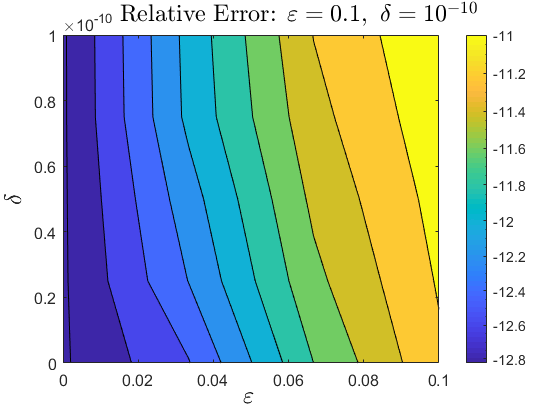
\includegraphics[width=7.6cm]{sections/7_conclusions_and_future_directions/Large_Eps_Small_Delta_2.png} }}%
    %\qquad
    \subfloat[\centering Small $\varepsilon$, Large $\delta$ ]{{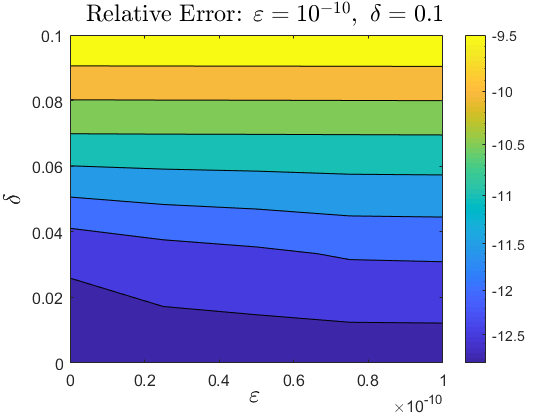
\includegraphics[width=7.6cm]{sections/7_conclusions_and_future_directions/Small_Eps_Large_Delta_2.png} }}%
    \vspace{3 mm}
    \caption{A contour plot of the relative error computed with our HOPS/AWE algorithm by holding $N=M=8$ Taylor orders fixed. In Figure $34\text{(a)}$ we expand up to $\Eps = 0.1$ and $\delta = 10^{-10}$ simultaneously with $N=M=8$ Taylor orders. In Figure $34\text{(b)}$ we expand up to $\Eps = 10^{-10}$ and $\delta = 0.1$ simultaneously with $N=M=8$ Taylor orders.}%
    \label{fig:example}%
\end{figure}
\vspace{-18mm}
Supplementary testing in both the upper and lower layers confirms that our HOPS/AWE algorithm is better suited towards larger $\varepsilon$.
%\begin{flushleft}
\newline
\\
\textbf{Predictions:} Our HOPS/AWE methodology takes advantage of exact enforcement of the \gls{owc} at an artificial boundary in order to truncate the computational domain to one of finite extent. After flattening the surface, the DNOs recover information through the solution stored at the interface. We suspect that this process mitigates large perturbations of the height/slope. By following techniques developed in \cite{NichollsReitich00b,NichollsTaber06,Nicholls16b,NichollsShen08}, we intend to rigorously prove that the TFE method is analytic when $\varepsilon$ is large. Additionally, we are interested in perturbing other physical parameters in the context of layered media problems. These are discussed in the engineering literature \cite{mashayekh2018parameter,mashayekh2018parameter2}.
\section{Rayleigh Singularities}
\label{Sec: Rayleigh Singularities}
A fundamental equation in the HOPS/AWE algorithm is
$$\alpha_p^2 + (\gamma_p^q(\delta))^2 = (k^q)^2,$$
where $k^q$ represents the wavenumber, $q\in\{u,w\}$, and $\alpha=k^q\sin(\theta), \gamma=k^q\cos(\theta),$ are parameters corresponding to refraction/reflection of the incidence angle $\theta$. As shown in $\S 5.4$, a Rayleigh singularity (or Wood's anomaly) occurs when $\ualpha_p^2 = (\uk^q)^2$ for any integer $p\neq 0$. That is, if $\ugamma_p^q(\delta) =0$ for $p\neq 0$ then the Taylor series expansion of $\gamma_p^q(\delta)$ is invalid. In \cite{Nicholls16}, the author investigated changing the Taylor expansion to a Puiseux expansion \cite{basu2007algorithms}:
$$\gamma_p^q(\delta)=\sum_{m=0}^{\infty}\gamma_{p,m}^q\delta^{m+1/2}=\delta^{1/2}\sum_{m=0}^{\infty}\gamma_{p,m}^q\delta^m.$$
However, he found that this approach ran into external difficulties ($\S$6 of \cite{Nicholls16}) simplifying explicit forms of the Dirichlet and Neumann trace operators.
\newline
\\
\textbf{Predictions:} Rayleigh singularities are a central obstruction to the convergence of our HOPS/AWE algorithm. In all of our numerical tests, we select custom frequency ranges which maximize the radius of convergence of our algorithm by expanding away from the singularities (cf. $\S 5.6$). Alternative methods such as Padé summation also fail to be analytic in a neighborhood of a Rayleigh singularity. General perturbation theory provides a variety of known techniques \cite{suslov2005divergent,convfromdiv,Heinz2020,dienes1957taylor,arteca1984summation} for expanding around divergent perturbation series. We suspect that adding these techniques to our HOPS/AWE algorithm will allow us perform a series expansion of $\ugamma_p^q(\delta)$ that does not diverge when $\ugamma_p^q(\delta)=0.$
\section{Multiple Layers}
\label{Sec: Multiple Layers}

In \cite{Nicholls16b}, the author discusses how to apply our HOPS methodology in multilayered configurations. He considers a multilayered material with $M$ (finite) interfaces at 
$$z=a^{(m)}+g^{(m)}(x,y),\quad 1\leq m \leq M,$$
which are $d_x \times d_y$ periodic
$$g^{(m)}(x+d_x,y+d_y)=g^{(m)}(x,y),\quad 1\leq m \leq M,$$
separating $(M+1)$--many layers.
%\vspace{-12mm}
\begin{figure}[H]
    \centering
    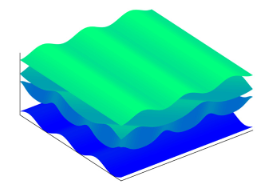
\includegraphics[width=7.6cm]{sections/7_conclusions_and_future_directions/multilayered.png}%
    \vspace{3mm}
    \caption{A five--layer problem configuration with layer interfaces $z = a^{(m)}+g^{(m)}(x).$}%
    \label{fig:example}%
\end{figure}
\vspace{-15mm}
%\begin{flushleft}
A generalization of our analyticity theorems (cf. $\S 4.5$) up to $M$ parameters is included as Theorem~$3.2$ in \cite{Nicholls16b}. For this, we consider quite general systems of linear equations of the form
%\end{flushleft}
\be
\bA(\tEps)\bV(\tEps)=\bR(\tEps),
\ee
where 
\bes
\bA(\tEps)=\sum_{\tn=0}^{\infty}\bA_{\tn}\tEps^{\tn},\quad 
\bR(\tEps) = \sum_{\tn=0}^{\infty}\bR_{\tn}\tEps^{\tn}.
\ees
The tildes represent multi--index notation \cite{Evans10}, in particular
\bes
\tEps := \begin{pmatrix} \Eps_1 \\ \vdots \\ \Eps_M \end{pmatrix},
\quad
\tn := \begin{pmatrix} n_1 \\ \vdots \\ n_M \end{pmatrix},
\ees
and the convention
\bes
\sum_{\tn=0}^{\infty} 
    A_{\tn}\ \tEps^{\tn}
  = \sum_{n_1=0}^{\infty} \cdots \sum_{n_M=0}^{\infty}
    A_{n_1,\ldots,n_M} \Eps_1^{n_1} \cdots \Eps_M^{n_M}.
\ees
As in $\S 4.5$, we seek a solution of the form
\be
\bV(\tEps)=\sum_{\tn=0}^{\infty}\bV_{\tn}\tEps^{\tn},
\ee
and from $(7.1)$ we find at order $\mathcal{O}(\tEps^{\tn})$
\bes
\bA_0\bV_{\tn}= \bR_{\tn} - \left(\sum_{\tl=0}^{\tn}\bA_{\tn-\tl}\bV_{\tl}- \bA_0\bV_{\tn}\right),
\ees
or
\be
\bV_{\tn}= \bA_0^{-1}\left\{\bR_{\tn} - \left(\sum_{\tl=0}^{\tn}\bA_{\tn-\tl}\bV_{\tl}- \bA_0\bV_{\tn}\right)\right\}.
\ee
The above notation represents multi--indices in the form
\bes
\sum_{\tl=0}^{\tn}\bA_{\tn-\tl}\bV_{\tl} = \sum_{\ell_1=0}^{n_1}\cdots \sum_{\ell_M=0}^{n_M}
    \bA_{n_1-\ell_1,\ldots,n_M-\ell_M} \bV_{\ell_1,\ldots,\ell_m},  
\ees
where $\tn=(n_1,\ldots,n_M),$ $\tl=(\ell_1,\ldots,\ell_M),$ and $0=(0,\ldots,0)$ with the convention
\bes
\tn \geq 0 \iff n_1\geq 0,\ldots,n_M\geq 0, \quad\tl \geq 0 \iff \ell_1\geq 0,\ldots,\ell_M\geq 0.
\ees
With these, we can extend our existence theorem (Theorem $4.5.1$) to $M$ parameters.
\begin{theorem}
\label{Thm:AVR}
Given two Banach spaces, $X$ and $Y$, suppose that:
\begin{enumerate}[label={\upshape[\arabic*]}]
\item $\bR_{\tn} \in Y$ for all $\tn \geq 0$,
  and there exist $M$--multi--indexed constants $C_R > 0$, $B_R > 0$,
  \bes
  C_R = \begin{pmatrix} C_{R,1} \\ \vdots \\ C_{R,M} \end{pmatrix},
  \quad
  B_R^{\tn} = \begin{pmatrix} B_{R,1}^{n_1} \\ \vdots \\ 
  B_{R,M}^{n_M} \end{pmatrix},
  \ees
  such that
  \bes
  \Norm{\bR_{\tn}}{Y} \leq C_R B_R^{\tn},
  \ees
\item $\bA_{\tn}: X \rightarrow Y$ for all
  $\tn \geq 0$, and there exist $M$--multi--indexed
  constants $C_A > 0$, $B_A > 0$ such that
  \bes
  \Norm{\bA_{\tn}}{X \rightarrow Y} \leq C_A B_A^{\tn},
  \ees
\item $\bA_0^{-1}: Y \rightarrow X$, and there 
  exists a constant $C_e > 0$ such that
  \bes
  \Norm{\bA_0^{-1}}{Y \rightarrow X} \leq C_e.
  \ees  
\end{enumerate}
Then the equation $(7.1)$ has a unique solution,
\be
\label{Eqn:V:Exp:Multi}
\bV(\tEps) = \sum_{\tn=0}^{\infty} \bV_{\tn} \tEps^{\tn},
\ee
and there exist $M$--multi--indexed constants $C_V > 0$ and $B_V > 0$ such that
\bes
\Norm{\bV_{\tn}}{X} \leq C_V B_V^{\tn},
\ees
for all $\tn \geq 0$ and any
\bes
C_V \geq 2 C_e C_R,
\quad
B_V \geq \max \left\{ B_R, 2 B_A, 2^{M+1} C_e C_A B_A \right\},
\ees
enforced componentwise. This implies that, for any $M$--multi--indexed constant
$0 \leq \tilde{\rho} < 1$, 
$(7.4)$, converges for all $\tEps$ such that
$B \tEps < \tilde{\rho}$, i.e., $\tEps < \tilde{\rho}/B$.
\end{theorem}
\begin{remark}
Our proof strategy is a form of multidimensional induction where given a statement $\bP(n_1, n_2, n_3, ..., n_M)$ for some $M\in \mathbb{N}$, we will show that $\forall n_1, n_2,\ldots, n_M \geq 0$, $\bP(n_1, n_2, n_3, ..., n_M)$ is true by inducting on $n_M$. We will follow the steps outlined below.
\begin{enumerate}
\item Establish $\bP(0,\ldots,n_j,\ldots,0)$ for all $1 \leq j < M$ and $n_1,\ldots,n_j \geq 0.$
\item Given $\bP(n_1,n_2,\ldots,n_j,\ldots,0)$ for all $1 \leq j < M$ and $n_1,\ldots,n_j \geq 0$, establish $\bP(n_1,n_2,\ldots,\bar{n}_j,\ldots,0)$. This can be accomplished through the two steps below.
\begin{enumerate}
    \item Establish $\bP(0,\ldots,\bar{n}_j,\ldots,0)$ for all $\bar{n}_j \geq 0$ (where the hypothesis in $[2]$ gives the required case for $n_j < \bar{n}_j$).
    \item Given  $\bP(n_1,n_2,\ldots,\bar{n}_j,\ldots,0)$ for all $1 \leq j < M$ and $n_1 < \bar{n}_1,  n_2 < \bar{n}_2,\ldots, $ $n_{j-1}  < \bar{n}_{j-1}$ and $\bar{n}_j\geq 0$, establish $\bP(\bar{n}_1,\bar{n}_2,\ldots,\bar{n}_j,\ldots,0)$.
\end{enumerate}
\item Given $\bP(n_1,n_2,\ldots,n_j,n_{j+1},\ldots,0)$ for all $1 \leq j+1 < M$ and $n_1,\ldots,n_{j+1} \geq 0$, establish $\bP(n_1,n_2,\ldots,n_j,\bar{n}_{j+1},\ldots,0)$. This can be accomplished by following the two steps outlined below. 
\begin{enumerate}
    \item Establish $\bP(0,\ldots,\bar{n}_{j+1},\ldots,0)$ for all $\bar{n}_{j+1} \geq 0$ (where the hypothesis in $[3]$ gives the required case for $n_{j+1} < \bar{n}_{j+1}$).
    \item Given  $\bP(n_1,n_2,\ldots,n_j,\bar{n}_{j+1},\ldots,0)$ for all $1 \leq j+1 < M$ and  $n_1 < \bar{n}_1,  n_2 < \bar{n}_2,\ldots, n_{j} < \bar{n}_{j}$ and $\bar{n}_{j+1}\geq 0$, establish $\bP(\bar{n}_1,\bar{n}_2,\ldots,\bar{n}_j,\bar{n}_{j+1}\ldots,0)$.
\end{enumerate}
\item Given $\bP(n_1,n_2,\ldots,n_{M-1},n_M)$ for all $n_1,n_2,\ldots,n_{M-1} \geq 0$ and $n_M < \bar{n}_M$, establish $\bP(n_1,n_2,\ldots,n_{M-1},\bar{n}_M)$. This can be accomplished by the two steps below (the base cases are handled through $[2]$ and $[3]$).
\begin{enumerate}
    \item Establish $\bP(0,\ldots,\bar{n}_{M})$ for $\bar{n}_{M} \geq 0$ (where the hypothesis in $[4]$ handles the required case for  $n_{M} < \bar{n}_{M}$).
    \item Given $\bP(n_1,n_2,\ldots,n_{M-1},\bar{n}_M)$ for all $n_1 < \bar{n}_1, n_2 < \bar{n}_2, \ldots n_{M-1} < \bar{n}_{M-1}$ and $\bar{n}_M \geq 0$, establish $\bP(\bar{n}_1,\bar{n}_2,\ldots,\bar{n}_{M-1},\bar{n}_M)$.
\end{enumerate}
\end{enumerate}

\end{remark}

\begin{proof}{[Theorem 7.4.1]} As with $\tEps$ and $\tn$, we represent $\tilde{\rho}$ by
\bes
\tilde{\rho} := \begin{pmatrix} \rho_1 \\ \vdots \\ \rho_M \end{pmatrix}.
\ees
As before, we will work by induction and consider the general case for finite $M>0$ where we want to establish
\bes
\norm{\bV_{n_1,\ldots,n_M}}_X \leq C_{V,1}\ldots C_{V,M} B_{V,1}^{n_1}\ldots B_{V,M}^{n_M}, \quad \forall n_1,\ldots,n_M\geq 0.
\ees
We prove this via an induction on $n_M$. The base case $n_1,n_2,\ldots, n_{j-1},n_{j+1},\ldots,$ $n_M=0$ and $1 \leq j < M$:
\bes
\norm{\bV_{0,\ldots,n_j,\ldots,0}}_X \leq C_{V,j} B_{V,j}^{n_j}, \quad \forall n_j\geq 0,
\ees
has previously been established by Theorem $4.5.1$ where $\tEps = \Eps_j$ and $\delta=0$. We now assume
\bes
\norm{\bV_{n_1,\ldots,n_j,\ldots,0}}_X \leq  C_{V,1}\ldots C_{V,j}B_{V,1}^{n_1}\ldots B_{V,j}^{n_j}, ~~ \forall n_1,\ldots,n_{j-1}\geq 0,~~ \forall n_j < \bar{n}_j,~~ 1 \leq j < M,
\ees
and seek
\bes
\norm{\bV_{n_1,\ldots,\bar{n}_j,\ldots,0}}_X \leq  C_{V,1}\ldots C_{V,j}B_{V,1}^{n_1}\ldots B_{V,j}^{\bar{n}_j}, ~~ \forall n_1,\ldots,n_{j-1}\geq 0.
\ees
This can be obtained through a chain of $(M-1)$ inductions on $n_1,\ldots,n_j$ where $1 \leq j < M$. For simplicity, we will show what happens in the arbitrary case $n_j$. The base case $n_1,\ldots,n_{j-1}=0$:
\bes
\norm{\bV_{0,\ldots,\bar{n}_j,\ldots,0}}_X \leq  C_{V,j}B_{V,j}^{\bar{n}_j}, \quad \forall \bar{n}_j \geq 0,
\ees
is established by Theorem $4.5.1$ where $\tEps = \Eps_j$ and $\delta=0$. Therefore, we assume
\begin{align*}
\norm{\bV_{n_1,\ldots,\bar{n}_j,\ldots,0}}_X \leq  C_{V,1}\ldots C_{V,j}B_{V,1}^{n_1}\ldots B_{V,j}^{\bar{n}_j},~~\forall n_1  &< \bar{n}_1,\ldots, n_{j-1} < \bar{n}_{j-1},~~ \forall \bar{n}_j \geq 0,\\&~ 1 \leq j < M,
\end{align*}
and seek
\bes
\norm{\bV_{\bar{n}_1,\ldots,\bar{n}_j,\ldots,0}}_X \leq  C_{V,1}\ldots C_{V,j}B_{V,1}^{\bar{n}_1}\ldots B_{V,j}^{\bar{n}_j}.
\ees
Recalling $\tn=(n_1,\ldots,n_j)$ and  $\tl=(\ell_1,\ldots,\ell_j)$, we define
\be
{\sum_{\tl=0}^{\tn}}^{*}\bA_{\tn-\tl}\bV_{\tl} := \sum_{\tl=0}^{\tn}\bA_{\tn-\tl}\bV_{\tl} - \bA_0\bV_{\tn},
\ee
and apply $(7.3),(7.5)$ and the mapping properties of $\bA_{0}^{-1}$ to find
\bes
\norm{\bV_{\bar{n}_1,\ldots,\bar{n}_j,\ldots,0}}_X\leq C_e\left\{\norm{\bR_{\bar{n}_1,\ldots,\bar{n}_j}}_Y + {\sum_{\tl=0}^{\tn}}^{*}\norm{\bA_{\tn-\tl}\bV_{\tl}}_Y\right\}.
\ees
Using the estimates on $\bR_{n_1,\ldots,n_j}$ and $\bA_{n_1,\ldots,n_j}$ (for all $n_1,\ldots,n_j$) and $\bV_{n_1,\ldots,n_j}$ $(n_1 < \bar{n}_1, \ldots, n_j < \bar{n}_j)$ we have
\begin{align*}
\norm{\bV_{\bar{n}_1,\ldots,\bar{n}_j,\ldots,0}}_X &\leq
C_e\Bigg\{C_{R,1}\ldots C_{R,j}B_{R,1}^{\bar{n}_1}\ldots B_{R,j}^{\bar{n}_j} + {\sum_{\tl=0}^{\tn}}^{*}C_{A,1}\ldots C_{A,j}B_{A,1}^{\bar{n}_1-\ell_1}\ldots B_{A,j}^{\bar{n}_j-\ell_j}\\ & \qquad \qquad \qquad \qquad \qquad \qquad \qquad \qquad \times
C_{V,1}\ldots C_{V,j}B_{V,1}^{\ell_1}\ldots B_{V,j}^{\ell_j}\Bigg\} \\& =
C_eC_{R,1}\ldots C_{R,j}B_{R,1}^{\bar{n}_1}\ldots B_{R,j}^{\bar{n}_j} + C_eC_{A,1}\ldots C_{A,j}C_{V,1}\ldots C_{V,j} \\&
~~ \times \left(\frac{B_{A,1}}{B_{V,1}}\right)B_{V,1}^{\bar{n}_1}\cdots \left(\frac{B_{A,j}}{B_{V,j}}\right)B_{V,j}^{\bar{n}_j}{\sum_{\tl=0}^{\tn}}^{*}
\left(\frac{B_{A,1}}{B_{V,1}}\right)B_{V,1}^{\bar{n}_1-\ell_1-1}\cdots \\& ~~ \times
\left(\frac{B_{A,j}}{B_{V,j}}\right)B_{V,j}^{\bar{n}_j-\ell_j-1} \\& \leq
C_eC_{R,1}\ldots C_{R,j}B_{V,1}^{\bar{n}_1}\ldots B_{V,j}^{\bar{n}_j} + C_eC_{A,1}\ldots C_{A,j}C_{V,1}\ldots C_{V,j} \\& ~~ \times
\left(\frac{B_{A,1}}{B_{V,1}}\right)B_{V,1}^{\bar{n}_1}\cdots\left(\frac{B_{A,j}}{B_{V,j}}\right)B_{V,j}^{\bar{n}_j}\left(\frac{1}{1-1/2}\right)^j,
\end{align*}
if $B_{A,k}/B_{V,k} \leq 1/2$, $k=1,\ldots,j$ (implying $B_{V,k} \geq 2B_{A,k}$). We are done if we demand that
\bes
B_{V,k} \geq B_{R,k}, \quad C_eC_{R,k} \leq C_{V,k}/2, \quad 2^jC_eC_{A,k}C_{V,k}(B_{A,k}/B_{V,k}) \leq 
C_{V,k}/2.
\ees
This can be realized if
\bes
C_{V,k} \geq 2C_eC_{R,k}, \quad
B_{V,k} \geq \max\left\{B_{R,k},2B_{A,k},2^{j+1}C_eC_{A,k}B_{A,k}\right\}.
\ees
We then assume
\begin{align*}
\norm{\bV_{n_1,\ldots,n_{j+1},\ldots,0}}_X \leq  C_{V,1}\ldots C_{V,j+1}B_{V,1}^{n_1}\ldots B_{V,j+1}^{n_{j+1}}, ~~ &\forall n_1,\ldots,n_j\geq 0,~~ \forall n_{j+1} < \bar{n}_{j+1},\\&~~ 1 \leq j < M,
\end{align*}
and seek
\bes
\norm{\bV_{n_1,\ldots,\bar{n}_{j+1},\ldots,0}}_X \leq  C_{V,1}\ldots C_{V,j+1}B_{V,1}^{n_1}\ldots B_{V,j+1}^{\bar{n}_{j+1}}, ~~ \forall n_1,\ldots,n_{j}\geq 0.
\ees
As before, this can be obtained through a chain of $M$ inductions on $n_1,\ldots,n_{j+1}$ where $1 \leq j < M$. For simplicity, we will show what happens in the arbitrary case $n_{j+1}$. The base case $n_1,\ldots,n_{j}=0$:
\bes
\norm{\bV_{0,\ldots,\bar{n}_{j+1},\ldots,0}}_X \leq  C_{V,j+1}B_{V,j+1}^{\bar{n}_{j+1}}, \quad \forall \bar{n}_{j+1} \geq 0,
\ees
is established by Theorem $4.5.1$ where $\tEps = \Eps_{j+1}$ and $\delta=0$. Therefore, we assume
\begin{align*}
\norm{\bV_{n_1,\ldots,\bar{n}_{j+1},\ldots,0}}_X \leq  C_{V,1}\ldots C_{V,j+1}B_{V,1}^{n_1}\ldots B_{V,j+1}^{\bar{n}_{j+1}},~~\forall n_1  &< \bar{n}_1,\ldots, n_{j} < \bar{n}_{j},~~ \forall \bar{n}_{j+1} \geq 0,\\&~ 1 \leq j < M,
\end{align*}
and seek
\bes
\norm{\bV_{\bar{n}_1,\ldots,\bar{n}_{j+1},\ldots,0}}_X \leq  C_{V,1}\ldots C_{V,j+1}B_{V,1}^{\bar{n}_1}\ldots B_{V,j+1}^{\bar{n}_{j+1}}.
\ees
In this scenario, $\tn=(n_1,\ldots,n_{j+1})$ and  $\tl=(\ell_1,\ldots,\ell_{j+1}),$ so we apply $(7.3),(7.5)$ and the mapping properties of $\bA_{0}^{-1}$ to find
\bes
\norm{\bV_{\bar{n}_1,\ldots,\bar{n}_{j+1},\ldots,0}}_X\leq C_e\left\{\norm{\bR_{\bar{n}_1,\ldots,\bar{n}_{j+1}}}_Y + {\sum_{\tl=0}^{\tn}}^{*}\norm{\bA_{\tn-\tl}\bV_{\tl}}_Y\right\}.
\ees
Using the estimates on $\bR_{n_1,\ldots,n_{j+1}}$ and $\bA_{n_1,\ldots,n_{j+1}}$ (for all $n_1,\ldots,n_{j+1}$) and $\bV_{n_1,\ldots,n_{j+1}}$ $(n_1 < \bar{n}_1, \ldots, n_{j+1} < \bar{n}_{j+1})$ we have
\begin{align*}
\norm{\bV_{\bar{n}_1,\ldots,\bar{n}_{j+1},\ldots,0}}_X &\leq
C_e\Bigg\{C_{R,1}\ldots C_{R,{j+1}}B_{R,1}^{\bar{n}_1}\ldots B_{R,{j+1}}^{\bar{n}_{j+1}} + {\sum_{\tl=0}^{\tn}}^{*}C_{A,1}\ldots C_{A,{j+1}}B_{A,1}^{\bar{n}_1-\ell_1}\ldots \\ & \qquad \qquad \qquad \qquad \qquad \quad \times
B_{A,{j+1}}^{\bar{n}_{j+1}-\ell_{j+1}}C_{V,1}\ldots C_{V,{j+1}}B_{V,1}^{\ell_1}\ldots B_{V,{j+1}}^{\ell_{j+1}}\Bigg\} \\& =
C_eC_{R,1}\ldots C_{R,{j+1}}B_{R,1}^{\bar{n}_1}\ldots B_{R,{j+1}}^{\bar{n}_{j+1}} + C_eC_{A,1}\ldots C_{A,{j+1}}C_{V,1}\ldots C_{V,{j+1}} \\&
~~ \times \left(\frac{B_{A,1}}{B_{V,1}}\right)B_{V,1}^{\bar{n}_1}\cdots \left(\frac{B_{A,{j+1}}}{B_{V,{j+1}}}\right)B_{V,{j+1}}^{\bar{n}_{j+1}}{\sum_{\tl=0}^{\tn}}^{*}
\left(\frac{B_{A,1}}{B_{V,1}}\right)B_{V,1}^{\bar{n}_1-\ell_1-1}\cdots \\& ~~ \times
\left(\frac{B_{A,{j+1}}}{B_{V,{j+1}}}\right)B_{V,{j+1}}^{\bar{n}_{j+1}-\ell_{j+1}-1} \allowdisplaybreaks\\& \leq
C_eC_{R,1}\ldots C_{R,{j+1}}B_{V,1}^{\bar{n}_1}\ldots B_{V,{j+1}}^{\bar{n}_{j+1}} + C_eC_{A,1}\ldots C_{A,{j+1}}C_{V,1}\ldots C_{V,{j+1}} \\& ~~ \times
\left(\frac{B_{A,1}}{B_{V,1}}\right)B_{V,1}^{\bar{n}_1}\cdots\left(\frac{B_{A,{j+1}}}{B_{V,{j+1}}}\right)B_{V,{j+1}}^{\bar{n}_{j+1}}\left(\frac{1}{1-1/2}\right)^{j+1},
\end{align*}
if $B_{A,t}/B_{V,t} \leq 1/2$, $t=1,\ldots,j+1$ (implying $B_{V,t} \geq 2B_{A,t}$). We are done if we demand that
\bes
B_{V,t} \geq B_{R,t}, \quad C_eC_{R,t} \leq C_{V,t}/2, \quad 2^{j+1}C_eC_{A,t}C_{V,t}(B_{A,t}/B_{V,t}) \leq 
C_{V,t}/2.
\ees
This can be realized if
\bes
C_{V,t} \geq 2C_eC_{R,t}, \quad
B_{V,t} \geq \max\left\{B_{R,t},2B_{A,t},2^{j+2}C_eC_{A,t}B_{A,t}\right\}.
\ees
To complete the general case for finite $M>0$, we assume
\bes
\norm{\bV_{n_1,\ldots,n_M}}_X \leq  C_{V,1}\ldots C_{V,M}B_{V,1}^{n_1}\ldots B_{V,M}^{n_M}, ~~ \forall n_1,\ldots,n_{M-1}\geq 0,~~ \forall n_M < \bar{n}_M,
\ees
and seek
\bes
\norm{\bV_{n_1,\ldots,\bar{n}_M}}_X \leq  C_{V,1}\ldots C_{V,M}B_{V,1}^{n_1}\ldots B_{V,M}^{\bar{n}_M}, ~~ \forall n_1,\ldots,n_{M-1}\geq 0.
\ees
The base case $n_1,n_2,\ldots,n_{M-1}=0$:
\bes
\norm{\bV_{0,\ldots,\bar{n}_M}}_X \leq  C_{V,M}B_{V,M}^{\bar{n}_M}, \quad \forall \bar{n}_M \geq 0,
\ees
has previously been established by Theorem $4.5.1$ where $\tEps = \Eps_M$ and $\delta =0$. Finally, we assume
\begin{align*}
\norm{\bV_{n_1,\ldots,n_{M-1},\bar{n}_M}}_X \leq  C_{V,1}\ldots C_{V,M}B_{V,1}^{n_1}\ldots B_{V,M}^{\bar{n}_M},~~~&\forall n_1  < \bar{n}_1,\ldots, n_{M-1} < \bar{n}_{M-1},\\&~~~~ \forall \bar{n}_M \geq 0,
\end{align*}
and seek
\bes
\norm{\bV_{\bar{n}_1,\ldots,\bar{n}_{M-1},\bar{n}_M}}_X \leq  C_{V,1}\ldots C_{V,M}B_{V,1}^{\bar{n}_1}\ldots B_{V,M}^{\bar{n}_M}.
\ees
In this case, $\tn=(n_1,\ldots,n_M)$ and  $\tl=(\ell_1,\ldots,\ell_M),$ so we apply $(7.3),(7.5)$ and the mapping properties of $\bA_{0}^{-1}$ to find
\bes
\norm{\bV_{\bar{n}_1,\ldots,\bar{n}_M}}_X\leq C_e\left\{\norm{\bR_{\bar{n}_1,\ldots,\bar{n}_M}}_Y + {\sum_{\tl=0}^{\tn}}^{*}\norm{\bA_{\tn-\tl}\bV_{\tl}}_Y\right\}.
\ees
Using the estimates on $\bR_{n_1,\ldots,n_M}$ and $\bA_{n_1,\ldots,n_M}$ (for all $n_1,\ldots,n_M$) and $\bV_{n_1,\ldots,n_M}$ $(n_1 < \bar{n}_1, \ldots, n_M < \bar{n}_M)$ we have
\vspace{-1.5mm}
\begin{align*}
\norm{\bV_{\bar{n}_1,\ldots,\bar{n}_M}}_X &\leq
C_e\Bigg\{C_{R,1}\ldots C_{R,M}B_{R,1}^{\bar{n}_1}\ldots B_{R,M}^{\bar{n}_M} + {\sum_{\tl=0}^{\tn}}^{*}C_{A,1}\ldots C_{A,M}B_{A,1}^{\bar{n}_1-\ell_1}\ldots B_{A,M}^{\bar{n}_M-\ell_M}\\ & \qquad \qquad \qquad \qquad \qquad \qquad \qquad \qquad \times
C_{V,1}\ldots C_{V,M}B_{V,1}^{\ell_1}\ldots B_{V,M}^{\ell_M}\Bigg\} \\& =
C_eC_{R,1}\ldots C_{R,M}B_{R,1}^{\bar{n}_1}\ldots B_{R,M}^{\bar{n}_M} + C_eC_{A,1}\ldots C_{A,M}C_{V,1}\ldots C_{V,M} \\& 
~~ \times \left(\frac{B_{A,1}}{B_{V,1}}\right)B_{V,1}^{\bar{n}_1}\cdots \left(\frac{B_{A,M}}{B_{V,M}}\right)B_{V,M}^{\bar{n}_M}{\sum_{\tl=0}^{\tn}}^{*}
\left(\frac{B_{A,1}}{B_{V,1}}\right)B_{V,1}^{\bar{n}_1-\ell_1-1}\cdots \\& \allowdisplaybreaks~~ \times
\left(\frac{B_{A,M}}{B_{V,M}}\right)B_{V,M}^{\bar{n}_M-\ell_M-1} \\&  \leq
C_eC_{R,1}\ldots C_{R,M}B_{V,1}^{\bar{n}_1}\ldots B_{V,M}^{\bar{n}_M} + C_eC_{A,1}\ldots C_{A,M}C_{V,1}\ldots C_{V,M} \\& ~~ \times
\left(\frac{B_{A,1}}{B_{V,1}}\right)B_{V,1}^{\bar{n}_1}\cdots\left(\frac{B_{A,M}}{B_{V,M}}\right)B_{V,M}^{\bar{n}_M}\left(\frac{1}{1-1/2}\right)^M,
\end{align*}
if $B_{A,i}/B_{V,i} \leq 1/2$, $i=1,\ldots,M$ (implying $B_{V,i} \geq 2B_{A,i}$). We are done if we demand that
\bes
B_{V,i} \geq B_{R,i}, \quad C_eC_{R,i} \leq C_{V,i}/2, \quad 2^MC_eC_{A,i}C_{V,i}(B_{A,i}/B_{V,i}) \leq 
C_{V,i}/2.
\ees
This can be realized if
\bes
C_{V,i} \geq 2C_eC_{R,i}, \quad
B_{V,i} \geq \max\left\{B_{R,i},2B_{A,i},2^{M+1}C_eC_{A,i}B_{A,i}\right\}.
\ees
\end{proof}
Using a similar approach in conjunction with the analysis in Chapters $2$ and $3$, we predict a more general form of Theorems $2.9.2$ and $3.8.1$ exists, which would establish the analyticity of the transformed field with respect to any finite $M > 0$ perturbation parameters.
\vspace{1mm}
\begin{conjecture} 
\label{Conj:u,w:Anal:n:n_m}
Given any integer $s \geq 0$, if $f \in C^{s+2}([0,d])$ and 
$U_{\tilde{n}} \in H^{s+3/2}([0,d])$, $W_{\tilde{n}}\in H^{s+3/2}([0,d])$ such that
\bes
\|U_{\tilde{n}}\|_{H^{s+3/2}} \le K_U B_U^{\tn} , \quad
\|W_{\tilde{n}}\|_{H^{s+3/2}} \le K_W B_W^{\tn} ,
\ees
for constants $K_U, K_W>0$ and $M$--multi--indexed constants $B_U, B_W > 0$, then 
$u_{\tn} \in H^{s+2}([0,d]\times[0,a])$, $w_{\tn}\in H^{s+2}([0,d]\times[-b,0])$ and
\bes
\label{Eqn:u,w:Est:n:n_m}
\|u_{\tn}\|_{H^{s+2}} \le K B^{\tn}, \quad
\|w_{\tn}\|_{H^{s+2}} \le \tilde{K}\tilde{B}^{\tn} ,
\ees
for constants $K,\tilde{K}> 0$ and $M$--multi--indexed constants $B ,\tilde{B}>0$.
\end{conjecture}
\vspace{1mm}
Analogously, a similar procedure would establish a more general form of Theorems $2.10.2$ and $3.9.2$ for the analyticity of the DNOs for any finite $M>0$ perturbation parameters.
\vspace{1mm}
\begin{conjecture} 
\label{Thm:G,J:Anal:n:n_m}
Given any integer $s \geq 0$, if $f \in C^{s+2}([0,d])$ and 
$U_{\tn} \in H^{s+3/2}([0,d])$, $W_{\tn} \in H^{s+3/2}([0,d])$ such that
\bes
\SobNorm{U_{\tn}}{s+3/2} \leq K_U B_U^{\tn}, \quad
\SobNorm{W_{\tn}}{s+3/2} \leq K_W B_W^{\tn},
\ees
for constants $K_U,K_W> 0$ and $M$--multi--indexed constants $B_U, B_W > 0$, then $G_{\tn} \in H^{s+1/2}([0,d])$, $J_{\tn} \in H^{s+1/2}([0,d])$ and
\bes
\label{Eqn:G,J:Est:n:n_m} 
\|G_{\tn}\|_{H^{s+1/2}} \le \tilde{K}\tilde{B}^{\tn}, \quad
\|J_{\tn}\|_{H^{s+1/2}} \le \dbtilde{K} \dbtilde{B}^{\tn},
\ees
for constants $\tilde{K},\dbtilde{K}  > 0$ and $M$--multi--indexed constants $\tilde{B},\dbtilde{B}>0$.
\end{conjecture}
\vspace{1mm}
Upon proving these, one has two key ingredients to the more general version of Theorem $4.6.1$ which establishes the existence and uniqueness of solutions to a system of partial differential equations with respect to $M$ perturbation parameters.
\vspace{1mm}
\begin{conjecture} 
\label{Conj:Main}
Given an integer $s \geq 0$, if $f \in C^{s+2}([0,d])$ then the 
equation $(7.1)$ has a unique solution, $(7.4)$,
and there exist a constant $C > 0$ and $M$--multi--indexed constants $B>0$ such that
\bes
\Norm{\bV_{\tn}}{X^s} \leq C B^{\tn},
\ees
for all $\tn \geq 0$.  This implies that for any $M$--multi--indexed constant
$0 \leq \tilde{\rho} < 1$, $(7.4)$, converges for all $\tEps$ such that
$B \tEps < \tilde{\rho}$, i.e., $\tEps < \tilde{\rho}/B$.
\end{conjecture}
\vspace{1mm}
\textbf{Predictions:} In application oriented fields such as signal processing or sea ice modeling, practitioners work with  multiple frequencies \cite{qiu2005high,bosse1995model,zhao2009multi,blanchard2021high} at short or long wavelengths. Also, as depicted in Figure $35$, the grating surface could have $M$ different layers \cite{imperatore2017perturbation} with distinct values of $g_j(x)=\Eps f_j(x),~j=1,\ldots, M$. A proof of Conjecture $7.4.4$ would enable the freedom to enforce any number of perturbation parameters and obtain an analytic solution. Given the widespread availability of parallel computing resources coupled with additional perturbation parameters associated with elastic media, we believe that future research will force hundreds or even thousands of distinct perturbation parameters, all of which should yield an analytic solution.
\section{Parallel Programming}
\setcounter{section}{5}
\label{Sec: Parallel Programming}

In the case of multiple layered interfaces, we need to compute intermediate DNOs for up to $M$ layers. This will greatly increase the computational cost and execution time of our HOPS/AWE algorithm and we suspect that it will be necessary to introduce parallel programming techniques to offset the computational expense. In the context of the \gls{oe} method, preliminary work \cite{fang2015operator} has been completed in C\texttt{++} to parallelize the computation of Navier's equations \cite{BillinghamKing00,achenbach2012wave}. These techniques can be adapted to the TFE method through the choice of OpenMP \cite{chandra2001parallel}, MPI \cite{snir1998mpi}, or CUDA \cite{sanders2010cuda}.
\newline
\\
\textbf{Predictions:} In two or three dimensions, our HOPS code is robust, efficient and has a runtime less than an hour. A local machine with an Intel Core i$5$ CPU, $8$GB of RAM, and Windows $10$ OS completed almost every simulation in this thesis in less than thirty minutes. However, with ten to one hundred layer configurations, we suspect that many simulations will take on the order of weeks or even months. As a result, it will be necessary to parallelize our Matlab code in a compiled programming language such as C or  C\texttt{++}.

\section{Alternatives to DNOs}
\label{Sec: Alternatives to DNOs}
In Chapter $4$ we wrote our scattering problem as a linear system
\bes
\bA \bV = \bR,
\ees
where, upon expanding $\{\bA,\bV,\bR\}$ in both $\varepsilon$ and $\delta$, we arrived at the flat--interface solution $\bA_{0,0}\bV_{0,0}=\bR_{0,0}$
at order $\mathcal{O}(\varepsilon^0,\delta^0)$. We then saw it was necessary to invert
\bes
\bA_{0,0} = \begin{pmatrix}I & -I\\
-G_{0,0} & -\tau^2J_{0,0}\end{pmatrix}, 
\ees
which features the two DNOs, $G_{0,0}$ and $J_{0,0}$, in order to show the existence and uniqueness of solutions. A primary feature of all HOPS schemes is the inversion of a single, sparse operator $\bA_{0,0}$ through the use of DNOs. However, one may ponder if a different technique could produce a more competitive algorithm that is comparable to our HOPS/AWE algorithm (or even better). Is it absolutely necessary to pass in transformed field data in order to efficiently compute and recover internal information stored at the grating surface?
\\
\newline
\textbf{Predictions:} A primary advantage of our HOPS/AWE scheme is that for every perturbation order, it is only necessary to invert a single sparse operator corresponding to a flat--interface, order--zero approximation. There are a number of competing approaches in general perturbation theory within the context of layered media problems. In regards to electromagnetic wave scattering, Galerkin and boundary element methods are discussed in \cite{escapil2020helmholtz,silva2017quantifying,nakata1990boundary,elschner2012optimization,rathsfeld2006} and a high--order perturbation approach based on boundary integral equations in \cite{dolz2020higher}. High--order schemes for linear waves can be computed using level set methods \cite{sethian1999level} and fast marching methods, as well as other methods involving domain decomposition \cite{el2004comparing,benamou1997domain,larsson1999domain,gong2021convergence,perez2018domain,chan1994domain}. A holistic evaluation of these competing methods could potentially improve our HOPS/AWE algorithm if we found a faster method of inverting linear operators without the use of DNOs.
\section{Computational Complexity}
\label{Sec: Computational Complexity}

One of the fundamental reasons for developing our HOPS/AWE algorithm is its advantageous computational complexity for problems within its domain of applicability.
In comparison with other classical methods, our HOPS/AWE approach has several advantages for computing quantities such as the Reflectivity Map, $R=R(\varepsilon,\delta)$. To demonstrate this we begin
by fixing the problem of computing $R$ for $N_{\Eps}$ many values of 
$\Eps$ and $N_{\delta}$ many values of $\delta$.

In the case of computing the DNOs $G$ and $J$, we recall from $\S 2.11$ and $\S 3.10$ that our HOPS/AWE algorithm requires
$N_x \times N_z$ unknowns at every perturbation order, $(n,m)$, corresponding to
the $N_x$ equally--spaced gridpoints in the lateral direction and the $N_z + 1$ collocation points in the vertical dimension. In $\S 4.5$ we saw that we could write our scattering problem as $\bA(\Eps,\delta) \bV(\Eps,\delta) = \bR(\Eps,\delta)$ where
\bes
    \bA(\Eps,\delta)=\sumn \summ \bA_{n,m}\Eps^n\delta^m, \quad \bR(\Eps,\delta) = \sumn \summ \bR_{n,m}\Eps^{n}\delta^m,
\ees
and
\bes
\label{Eqn:Soln:Two_Param_Append}
\bV(\Eps,\delta) = \sumn \summ \bV_{n,m}\Eps^{n}\delta^m.
\ees
At order $\mathcal{O}(\Eps^n,\delta^m)$ this becomes
\begin{align}
\begin{split}
\bA_{0,0}\bV_{n,m}=&~\bR_{n,m}-\sum_{\ell=0}^{n-1}\bA_{n-\ell,0}\bV_{\ell,m}-\sum_{r=0}^{m-1}\bA_{0,m-r}\bV_{n,r}\\&
-\sum_{\ell=0}^{n-1}\sum_{r=0}^{m-1}\bA_{n-\ell,m-r}\bV_{\ell,r}.
\end{split}
\end{align}
A careful study of $(7.6)$
reveals that the computational complexity of forming the
right--hand side at order $(n,m)$ is
\bes
\BigOh{n m N_x \log(N_x) N_z \log(N_z)}.
\ees
Inverting the operator $\bA_{0,0}$ has complexity $\BigOh{N_x \log(N_x) N_z \log(N_z)}$
so the full cost of computing the $\bV_{n,m}$, 
$\{ 0 \leq n \leq N, 0 \leq m \leq M \}$, is
\bes
\BigOh{N^2 M^2 N_x \log(N_x) N_z \log(N_z)}.
\ees
Once these coefficients are recovered, the cost of summing the series in 
$(\Eps,\delta)$ is minimal, provided it is done in an efficient manner 
(e.g., by Horner's rule \cite{BurdenFaires,AtkinsonHan01}). Our algorithm then 
requires an additional $\BigOh{N_{\Eps} N_{\delta}}$ steps to sum 
over every value of $(\Eps,\delta)$, therefore the full cost of 
computing the Reflectivity Map by our HOPS/AWE method is
\be
\BigOh{N^2 M^2 N_x \log(N_x) N_z \log(N_z) + N_{\Eps} N_{\delta}}.
\ee
In contrast, for a single $(\Eps,\delta)$ pair, a Boundary Integral Method solver with $N_x$ lateral
gridpoints requires time proportional to $\BigOh{N_x^3}$ for Gaussian elimination
to solve the resulting dense system of $N_x$ equations in $N_x$ unknowns
\cite{BurdenFaires,AtkinsonHan01,ColtonKress13}. Applying this 
$N_{\Eps} \times N_{\delta}$ times results in a total computational complexity of
\be
\BigOh{N_x^3 N_{\Eps} N_{\delta}}.
\ee
Thus, once $N_{\Eps}$ and $N_{\delta}$ become large, e.g.,

\bes
N_{\Eps} N_{\delta} > \frac{N^2 M^2 N_x \log(N_x) N_z \log(N_z)}{N_x^3},
\ees
our new algorithm becomes far more efficient. We speculate that the cost of $(7.7)$ could be reduced to
\be
\BigOh{N M \log(NM)N_x \log(N_x) N_z \log(N_z) + N_{\Eps} N_{\delta}},
\ee
provided that we develop a more efficient method of computing the $\bV_{n,m}$, 
$\{ 0 \leq n \leq N, 0 \leq m \leq M \}$, such as reducing the problem space at every step. Alternative approaches to layered media problems have also been proposed by other authors \cite{bai2004reduction,chew2005fast}, including interpolation \cite{atkins2010fast} and Green's function \cite{konno2016fast}.
\newline
\\
\textbf{Predictions:} The combination of implementing parallel programming techniques (through, e.g., OpenMP or CUDA) and reducing the problem space at every step will greatly enhance the speed and fidelity of our HOPS/AWE algorithm. Considering the natural advantage surface methods have over conventional methods, such as finite difference, finite element, and spectral element methods, we expect that our HOPS/AWE algorithm will be among the most competitive available for periodic layered media problems.
\newpage
\phantomsection
\appendices
\appendix

\chapter{Matlab Code}
\label{Appendix A: Matlab Code}
\thispagestyle{pageonbottom}

\pagestyle{fancy}
\renewcommand{\sectionmark}[1]{\markright{#1}}
\fancyhead{}
%%%%%%%%%%%%%%%%%%%%%%%%%%%% The paper headers
\fancyhead[LE,RO]{\thepage}
\fancyhead[LO]{\text{Appendix A} \quad   {Matlab Code}}
\fancyhead[RE]{\text{Appendix A} \quad   {Matlab Code}} %Even page header and number at left top
\fancyfoot[L,R,C]{}
\renewcommand{\headrulewidth}{1pt}% disable the underline of the header part
%\end{flushleft}
We present a subset of the Matlab code used to simulate our numerical results. Three essential algorithms used to define the upper and lower fields are the computation of the flat--interface solution of $\bA_{0,0}$, the upper and lower layer DNOs, $G_{n,m}=G_{n,m}(x;\Eps,\delta)$ and $J_{n,m}=J_{n,m}(x;\Eps,\delta)$, and the upper and lower transformed field solvers, $u_{n,m}=$ $u_{n,m}(x,z;\Eps,\delta)$ and $w_{n,m}=w_{n,m}(x,z;\Eps,\delta)$. In Algorithm $\text{A}.0.1$ we show our technique for inverting the flat--interface solution of $\bA_{0,0}$ (cf. $\S 4.8$).
\vspace{-15mm}
\begin{algorithm}[H]
\caption{Inversion of the flat--interface operator $\bA_{0,0}$}
\label{alg:inverse_ao}
\begin{algorithmic}[1]
\State $\text{Set $Nx$: The number of discretization points}$
\State $\text{Set $i\gamma_p^u$: The Fourier multiplier for $G_{0,0}$}$
\State $\text{Set $i\gamma_p^w$: The Fourier multiplier for $J_{0,0}$}$
\State $\text{Set $\gamma^q=(1+\delta)\ugamma^q,q\in\{u,w\},$ where $\delta$ represents a small frequency perturbation}$
\State $\text{Set $\tau$: Constant representing TE or TM polarization mode}$
\State $\zeta_{0,0} \in\mathbb R^{N_x},~\psi_{0,0} \in\mathbb R^{N_x} $
\vspace{0.5mm}
\State $\widehat{\zeta}_{0,0} \in\mathbb C^{N_x},~\widehat{\psi}_{0,0} \in\mathbb C^{N_x} $
\For{$j=1:Nx$} \do ${\boldsymbol{\rightarrow} \text{Entries of $\left[ \widehat{\bA}_{0,0}(p) \right]^{-1} $}}$
\State $\operatorname{det}_p = -\left\{i\ugamma_p^u(j) + \tau^2\left( i\ugamma_p^w(j)\right)\right\}$
\State $\underline{a}(j) = \left[\tau^2\left( -i\ugamma_p^w(j)\right)\widehat{\zeta}_{0,0}(j) + \widehat{\psi}_{0,0}(j)\right]/\operatorname{det}_p $
\State $\underline{b}(j) = \left[\left(i\ugamma_p^u(j)\right)\widehat{\zeta}_{0,0}(j) + \widehat{\psi}_{0,0}(j)\right]/\operatorname{det}_p $
\EndFor
\State $U_{0,0}=\operatorname{IFFT}(\underline{a}), ~ W_{0,0}=\operatorname{IFFT}(\underline{b})$
\State\Return $U_{0,0}, W_{0,0}$
\end{algorithmic}
\end{algorithm}
\vspace{-17mm}
Next, Algorithm $\text{A}.0.2$ demonstrates how we calculate the upper layer DNO, $G$ (cf. $\S 2.10$ and $\S 2.11$).
\vspace{-14mm}
\begin{algorithm}[H]
\caption{Computation of the upper layer DNO, $G$}
\label{alg:dno}
\begin{algorithmic}[1]
\State $\text{Set $Nx$: The number of discretization points}$
\State $\text{Set $Nz$: The number of collocation points}$
\State $\text{Set $N$: The maximum number of Taylor orders for the interfacial perturbation}$
\State $\text{Set $M$: The maximum number of Taylor orders for the frequency perturbation}$
\State $\text{Set $dx$: The partial derivative with respect to the $x$ component}$
\State $\text{Set $dz$: The partial derivative with respect to the $z$ component}$
\State $\text{Set $a$: The artificial boundary imposed at the top of the upper layer}$
\algstore{myalg}
\end{algorithmic}
\end{algorithm}

\begin{algorithm}                     
\begin{algorithmic}[1]
\algrestore{myalg}
\State $\text{Set $\tilde{p}=(2\pi/d)p$ for an integer $p$ where $d$ is the periodicity of the grating interface}$
\State $\text{Set $f=\sin(x)$, or a similar test function representing the grating surface}$
\State $\text{Set $f_x:$ The derivative of $f$ with respect to the $x$ component}$
\State $\text{Set $\ell_{\text{bottom}}=Nz+1,$ the bottom or last collocation point on the $z$--axis}$
\State $u_{n,m}\in\mathbb C^{N_x\times (N_z+1) \times (M+1) \times (N+1)}, ~ G_{n,m} \in\mathbb C^{N_x\times (M+1) \times (N+1)} $
\State $u_x\in\mathbb C^{N_x \times (N_z+1)}, ~ u_z \in\mathbb C^{N_x \times (N_z+1)}$
\For{$n=1:N$}
\For{$m=1:M$} ${\boldsymbol{\rightarrow} \text{Order $(n,m)$ terms in equation $(2.52)$ in $\S 2.10 $}}$
\State $u_z = dz(u_{n,m}(:,:,m,n),a)$
\State $G_{n,m}(:,m,n) = -u_z(:,\ell_{\text{bottom}}) $
\If{$n > 1$} ${\boldsymbol{\rightarrow} \text{Order $(n-1,m)$ terms in equation $(2.53)$ in $\S 2.10 $}}$
\State $u_x = dx(u_{n,m}(:,:,m,n-1),\tilde{p})$
\State $G_{n,m}(:,m,n) = G_{n,m}(:,m,n) + f_xu_x(:,\ell_{\text{bottom}})$
\State $G_{n,m}(:,m,n) = G_{n,m}(:,m,n) + (1/a)\cdot (f\cdot G_{n,m}(:,m,n-1))$
\EndIf
\If{$n >2$} ${\boldsymbol{\rightarrow} \text{Order $(n-2,m)$ terms in equation $(2.53)$ in $\S 2.10 $}}$
\State $u_x = dx(u_{n,m}(:,:,m,n-2),\tilde{p})$
\State $G_{n,m}(:,m,n) = G_{n,m}(:,m,n) - (1/a)\cdot(ff_x\cdot u_x(:,\ell_{\text{bottom}}))$
\State $u_z = dz(u_{n,m}(:,:,m,n-2),a)$
\State $G_{n,m}(:,m,n) = G_{n,m}(:,m,n) - (f_x^2\cdot u_z(:,\ell_{\text{bottom}}))$
\EndIf
\EndFor
\EndFor
\State\Return $G_{n,m}$
\end{algorithmic}
\end{algorithm}
\vspace{-18mm}
Lastly, Algorithm $\text{A}.0.3$ summarizes how we compute the upper transformed field, $u$ (cf. $\S 2.4$, $\S 2.6$, and $\S 2.11$). Due to its complexity and length, we leave out some details to the Matlab implementation in Listing $\text{A}.1$. 
\vspace{-14mm}
\begin{algorithm}[H]
\caption{Computation of the upper transformed field, $u$}
\label{alg:transformed_field}
\begin{algorithmic}[1]
\State $\text{Set $Nx$: The number of discretization points}$
\State $\text{Set $Nz$: The number of collocation points}$
\State $\text{Set $N$: The maximum number of Taylor orders for the interfacial perturbation}$
\State $\text{Set $M$: The maximum number of Taylor orders for the frequency perturbation}$
\State $\text{Set $dx$: The partial derivative with respect to the $x$ component}$
\State $\text{Set $dz$: The partial derivative with respect to the $z$ component}$
\State $\text{Set $a$: The artificial boundary imposed at the top of the upper layer}$
\State $\text{Set $\tilde{p}=(2\pi/d)p$ for an integer $p$ where $d$ is the periodicity of the grating interface}$
\State $\text{Set $f=\cos(x)$, or a similar test function representing the grating surface}$
\State $\text{Set $f_x:$ The derivative of $f$ with respect to the $x$ component}$
\State $\text{Set $\ell_{\text{top}}=0+1,$ the top or first collocation point on the $z$--axis}$
\State $\text{Set $T^u:$ Expansion of frequency operator, cf. $\S 5.4$}$
\State $\text{Set $g(x)=\Eps f(x),$ where $\Eps$ represents a small interfacial perturbation}$
\State $\text{Set $\gamma^u=(1+\delta)\ugamma^u$, $\alpha = (1+\delta)\ualpha$,
where $\delta$ is a small frequency perturbation}$
\algstore{myalg_2}
\end{algorithmic}
\end{algorithm}

\begin{algorithm}[H]                    
\begin{algorithmic}[1]
\algrestore{myalg_2}
\State $\text{Set $z'=a(z-g(x))/(a-g(x)),$ per transformation rules in $\S 2.4.$ Relabel $z=z'$}$
\State $\xi_{n,m}\in\mathbb R^{N_x \times (M+1) \times (N+1)}, ~ \widehat{\xi}_{n,m}\in \mathbb C^{N_x \times (M+1) \times (N+1)} $
\State $U_{n,m}\in  \mathbb R^{N_x \times (N_z+1)},~ \widehat{U}_{n,m}\in  \mathbb C^{N_x \times (N_z+1)}$
\State $ F_{n,m}\in\mathbb R^{N_x \times (N_z+1)}, ~ \widehat{F}_{n,m}\in\mathbb C^{N_x \times (N_z+1)}$
\State $u_{n,m}\in\mathbb C^{N_x\times (N_z+1) \times (M+1) \times (N+1)}, ~J_{n,m}\in\mathbb R^{N_x}, ~ \widehat{J}_{n,m}\in\mathbb C^{N_x}$
\State $\text{Compute $A_1^{xx},A_1^{xz},A_1^{zx},A_1^{zz},A_2^{xx},A_2^{xz},A_2^{zx},A_2^{zz},B_1^{x},B_1^{z},B_2^{x},B_2^{z},S_0,S_1$, and}$
\State ${\text{$S_2$ through equations $(2.16)$ in $\S 2.4$}}$
\For{$n=1:N$}
\For{$m=1:M$}
\If{$n >  1$} ${\boldsymbol{\rightarrow} \text{Order $(n-1,m)$ terms in equation $(2.28)$ in $\S 2.6 $}}$
\State $u_x = dx(u_{n,m}(:,:,m,n-1),\tilde{p})$
\State $F_{n,m} = F_{n,m} - dx(A_1^{xx}\cdot u_x,\tilde{p})$
\State $F_{n,m} = F_{n,m} - dz(A_1^{zx}\cdot u_x,a)$
\State $F_{n,m} = F_{n,m} - B_1^{x}\cdot u_x$
\State $u_z = dz(u_{n,m}(:,:,m,n-1),a)$
\State $F_{n,m} = F_{n,m} - dx(A_1^{xz}\cdot u_z,\tilde{p})$
\State $F_{n,m} = F_{n,m} - (2i\ualpha)\cdot S_1 \cdot u_x $
\State $F_{n,m} = F_{n,m} - (\ugamma^u)^2\cdot S_1 \cdot u_{n,m}(:,:,m,n-1)$
\EndIf
\If{$m > 1$} ${\boldsymbol{\rightarrow} \text{Order $(n,m-1)$ terms in equation $(2.28)$ in $\S 2.6 $}}$
\State $u_x = dx(u_{n,m}(:,:,m-1,n),\tilde{p})$
\State $F_{n,m} = F_{n,m} - (2i\ualpha)\cdot u_x$
\State $F_{n,m} = F_{n,m} - (2(\ugamma^u)^2)\cdot u_{n,m}(:,:,m-1,n)$
\EndIf
\If{$n>1 \text{ and } m>1$} ${\boldsymbol{\rightarrow} \text{Order $(n-1,m-1)$ terms in equation $(2.28)$}}$
\State $u_x = dx(u_{n,m}(:,:,m-1,n-1),\tilde{p})$
\State $F_{n,m} = F_{n,m} - (2i\ualpha)\cdot S_1 \cdot u_x$
\State $F_{n,m} = F_{n,m} - (2(\ugamma^u)^2)\cdot S_1 \cdot u_{n,m}(:,:,m-1,n-1)$
\EndIf
\If{$n>2$} ${\boldsymbol{\rightarrow} \text{Order $(n-2,m)$ terms in equation $(2.28)$ in $\S 2.6 $}}$
\State $u_x = dx(u_{n,m}(:,:,m,n-2),\tilde{p})$
\State $F_{n,m} = F_{n,m} - dx(A_2^{xx}\cdot u_x,\tilde{p})$
\State $F_{n,m} = F_{n,m} - dz(A_2^{zx}\cdot u_x,a)$
\State $F_{n,m} = F_{n,m} - B_2^x \cdot u_x$
\State $u_z = dz(u_{n,m}(:,:,m,n-2),a)$
\State $F_{n,m} = F_{n,m} - dx(A_2^{xz} \cdot u_z,\tilde{p})$
\State $F_{n,m} = F_{n,m} - dz(A_2^{zz} \cdot u_z,a)$
\State $F_{n,m} = F_{n,m} - B_2^z \cdot u_z - (2i\ualpha)\cdot S_2 \cdot u_x$
\State $F_{n,m} = F_{n,m} - (\ugamma^u)^2 \cdot S_2 \cdot u_{n,m}(:,:,m,n-2)$
\EndIf
\algstore{myalg_2}
\end{algorithmic}
\end{algorithm}

\begin{algorithm}[H]                    
\begin{algorithmic}[1]
\algrestore{myalg_2}
\If{$m > 2$} ${\boldsymbol{\rightarrow} \text{Order $(n,m-2)$ terms in equation $(2.28)$ in $\S 2.6 $}}$
\State $F_{n,m} = F_{n,m} - (\ugamma^u)^2\cdot u_{n,m}(:,:,m-2,n)$
\EndIf
\If{$n>1 \text{ and } m > 2$} ${\boldsymbol{\rightarrow} \text{Order $(n-1,m-2)$ terms in equation $(2.28)$ }}$
\State $F_{n,m} = F_{n,m} - (\ugamma^u)^2 \cdot S_1 \cdot u_{n,m}(:,:,m-2,n-1)$
\EndIf
\If{$n > 2 \text{ and } m>1$} ${\boldsymbol{\rightarrow} \text{Order $(n-2,m-1)$ terms in equation $(2.28)$ }}$
\State $u_x = dx(u_{n,m}(:,:,m-1,n-2),\tilde{p})$
\State $F_{n,m} = F_{n,m} - (2i\ualpha)\cdot S_2 \cdot u_x$
\State $F_{n,m} = F_{n,m} - (2(\ugamma^u)^2) \cdot S_2 \cdot u_{n,m}(:,:,m-1,n-2)$
\EndIf
\If{$n>2 \text{ and } m > 2$} ${\boldsymbol{\rightarrow} \text{Order $(n-2,m-2)$ terms in equation $(2.28)$ }}$
\State $F_{n,m} = F_{n,m} - (\ugamma^u)^2 \cdot S_2 \cdot u_{n,m}(:,:,m-2,n-2)$
\EndIf
\For{$r=0:m-1$} ${\boldsymbol{\rightarrow} \text{Transparent boundary condition, $(2.29)$ in $\S 2.6$ }}$
\State $J_{n,m} = J_{n,m} + \operatorname{IFFT}( (T^u(:,m-r))\cdot \operatorname{FFT}(u_{n,m}(:,\ell_{\text{top}},r,n)))$
\EndFor
\If{$n > 1$}
\For{$r=0:m$} ${\boldsymbol{\rightarrow} \text{Transparent boundary condition, $(2.29)$ in $\S 2.6$ }}$
\State $S_{n,m} = \operatorname{IFFT}( T^u(:,m-r))\cdot \operatorname{FFT}(u_{n,m}(:,\ell_{\text{top}},r,n-1)) )$
\State $J_{n,m} = J_{n,m} - (1.0/a)\cdot f \cdot S_{n,m}$
\EndFor
\EndIf
\State $\widehat{F}_{n,m} = \operatorname{FFT}(F_{n,m}), ~ \widehat{J}_{n,m} = \operatorname{FFT}(J_{n,m})$
\State $\widehat{U}_{n,m} = \text{Chebyshev collocation method of parameters in $(2.63)$ of $\S 2.11$}$
\If{$n>0 \text{ or } m>0}$
\State $u_{n,m}(:,:,m,n)=\operatorname{IFFT}(\widehat{U}_{n,m})$
\EndIf
\EndFor
\EndFor
\State\Return $u_{n,m}$
\end{algorithmic}
\end{algorithm}
\vspace{-19mm}
We now turn to example Matlab implementations. Our first script is the code for the upper transformed field, $u=u(x,y;\varepsilon,\delta)$ (cf. Algorithm $\text{A}.0.3$). A computational novelty of our HOPS/AWE algorithm is the speed at which we can compute the flat--interface solution in Fourier space by inverting a sparse operator at every wavenumber. To do this, we apply the \gls{fft} and \gls{ifft} in Matlab. Because Matlab array indices start from $1$ (linear indexing), we will add ``$+1$'' in all of the loop variables executed in our Matlab scripts.

%\begin{singlespacing}
\begin{lstlisting}[caption={Upper Field Solver for the TFE Method},frame=single]
function [unm] = field_tfe_helmholtz_m_and_n(xi_n_m,f,p,gammap,alpha,...
        gamma,Dz,a,Nx,Nz,N,M,identy)

unm = zeros(Nx,Nz+1,M+1,N+1);

k2 = p(0+1)^2 + gammap(0+1)^2;

ell_top = 0 + 1;
xi_n_m_hat = 0*xi_n_m;
for n=0:N
  for m=0:M
    xi_n_m_hat(:,m+1,n+1) = fft(xi_n_m(:,m+1,n+1));
  end
end
f_x = real(ifft((1i*p).*fft(f)));

ll = [0:Nz]';
z_min = 0; z_max = a;
D = (2/(z_max-z_min))*Dz;
D2 = D*D;
D_start = D(1,:);
D_end = D(end,:);
tilde_z = cos(pi*ll/Nz);
z = ((z_max-z_min)/2.0)*(tilde_z - 1.0) + z_max;

f_full = repmat(f,1,Nz+1);
f_x_full = repmat(f_x,1,Nz+1);
a_minus_z_full = repmat(a - z.',Nx,1);

Uhat = zeros(Nx,Nz+1);

Tu = Tu_dno(alpha,p,gamma,gammap,k2,Nx,M);

% n=0 and m=0

for ell=0:Nz
  unm(:,ell+1,0+1,0+1) = ifft(exp(1i*gammap*z(ell+1)).*xi_n_m_hat(:,0+1,0+1));
end

A1_xx = -(2.0/a)*f_full;
A1_xz = -(1.0/a)*(a_minus_z_full).*f_x_full;
A1_zx = A1_xz;
%A1_zz = 0;
  
A2_xx = (1.0/a^2)*f_full.^2;
A2_xz = (1.0/a^2)*(a_minus_z_full).*(f_full.*f_x_full);
A2_zx = A2_xz;
A2_zz = (1.0/a^2)*((a_minus_z_full).^2).*(f_x_full.^2);
  
B1_x = (1.0/a)*f_x_full;
%B1_z = 0;
  
B2_x = -(1.0/a^2)*f_full.*f_x_full;
B2_z = -(1.0/a^2).*(a_minus_z_full).*(f_x_full.^2);

S1 = -(2.0/a)*f_full;
S2 = (1.0/a^2)*f_full.^2;

for n=0:N
  for m=0:M
    
    % Form Fnm, Jnm
    Fnm = zeros(Nx,Nz+1);
    Jnm = zeros(Nx,1);
    
    if(n>=1)
      u_x = dx(unm(:,:,m+1,n-1+1),p);
      temp = A1_xx.*u_x;
      Fnm = Fnm - dx(temp,p);
      temp = A1_zx.*u_x;
      Fnm = Fnm - dz(temp,Dz,a);
      temp = B1_x.*u_x;
      Fnm = Fnm - temp;
    
      u_z = dz(unm(:,:,m+1,n-1+1),Dz,a);
      temp = A1_xz.*u_z;
      Fnm = Fnm - dx(temp,p);
      %A1_zz = 0
      %B1_z = 0
    
      temp = 2*1i*alpha.*S1.*u_x;
      Fnm = Fnm - temp;
	  temp = gamma^2.*S1.*unm(:,:,m+1,n-1+1);
	  Fnm = Fnm - temp;
    end
	
 	if(m>=1)
 	  u_x = dx(unm(:,:,m-1+1,n+1),p);
 	  temp = 2*1i*alpha.*u_x;
 	  Fnm  = Fnm - temp;
 	  temp = 2*gamma^2.*unm(:,:,m-1+1,n+1);
 	  Fnm  = Fnm - temp;
 	end
	
 	if(n>=1 && m>=1)
 	  u_x = dx(unm(:,:,m-1+1,n-1+1),p);
 	  temp = 2*1i*alpha.*S1.*u_x;
 	  Fnm  = Fnm - temp;
 	  temp = 2*gamma^2.*S1.*unm(:,:,m-1+1,n-1+1);
 	  Fnm  = Fnm - temp;
 	end
	 
    if(n>=2)
      u_x = dx(unm(:,:,m+1,n-2+1),p);
      temp = A2_xx.*u_x;
      Fnm = Fnm - dx(temp,p);
      temp = A2_zx.*u_x;
      Fnm = Fnm - dz(temp,Dz,a);
      temp = B2_x.*u_x;
      Fnm = Fnm - temp;
    
      u_z = dz(unm(:,:,m+1,n-2+1),Dz,a);
      temp = A2_xz.*u_z;
      Fnm = Fnm - dx(temp,p);
      temp = A2_zz.*u_z;
      Fnm = Fnm - dz(temp,Dz,a);
      temp = B2_z.*u_z;
      Fnm = Fnm - temp;
    
      temp = 2*1i*alpha.*S2.*u_x;
      Fnm = Fnm - temp;
	  temp = gamma^2.*S2.*unm(:,:,m+1,n-2+1);
	  Fnm = Fnm - temp;
    end
	
    if(m>=2)
 	  temp = gamma^2.*unm(:,:,m-2+1,n+1);
 	  Fnm = Fnm - temp;
    end
 	
    if(n>=1 && m>=2)
 	 temp = gamma^2.*S1.*unm(:,:,m-2+1,n-1+1);
 	 Fnm = Fnm - temp;
    end
 	
    if(n>=2 && m>=1)
 	 u_x = dx(unm(:,:,m-1+1,n-2+1),p);
 	 temp = 2*1i*alpha.*S2.*u_x;
 	 Fnm = Fnm - temp;
 	 temp = 2*gamma^2.*S2.*unm(:,:,m-1+1,n-2+1);
 	 Fnm = Fnm - temp;
    end
 	
    if(n>=2 && m>=2)
 	 temp = gamma^2.*S2.*unm(:,:,m-2+1,n-2+1);
 	 Fnm = Fnm - temp;
    end
     
    for r=0:m-1
      Jnm = Jnm + ifft((Tu(:,m-r+1)).*fft(unm(:,ell_top,r+1,n+1)));
    end
    if(n>=1)
      for r=0:m
        Snm = ifft((Tu(:,m-r+1)).*fft(unm(:,ell_top,r+1,n-1+1)) );
        Jnm = Jnm - (1.0/a)*f.*Snm;
      end
    end
    
    % Solve elliptic equation
    
    Fnmhat = fft(Fnm);
    Jnmhat = fft(Jnm);
    
    b = Fnmhat.';
    alphaalpha = 1.0;
    betabeta = 0.0;
    gammagamma = gamma*gamma - p.^2 - 2*alpha.*p;
    d_min = 1.0;
    n_min = 0.0;
    r_min = xi_n_m_hat(:,m+1,n+1);
    d_max = -1i*gammap;
    n_max = 1.0;
    r_max = Jnmhat;
    
    % Solve BVP through the Chebyshev collocation method
    
    Uhat = solvebvp_colloc(Uhat,b,alphaalpha,betabeta,gammagamma,...
        d_min,n_min,r_min,d_max,n_max,r_max,Nx,identy,D,D2,D_start,D_end);
    
    if((n>0)||(m>0))
      unm(:,:,m+1,n+1)=ifft(Uhat);
    end
    
  end
end

return;
\end{lstlisting}
%\end{singlespacing}
Our next script shows how we use the boundary data from the upper field solver to calculate the transformed field in Fourier space. We recover field data by inverting this operation for every perturbation order of $\varepsilon$ and $\delta$.

%\begin{singlespacing}
\begin{lstlisting}[caption={BVP Solver for the Chebyshev Collocation Method},frame=single]
function [Uhat] = solvebvp_colloc(Uhat,b,alpha,beta,gamma,d_min,n_min,...
    r_min,d_max,n_max,r_max,Nx,identy,D,D2,D_start,D_end)

A = alpha*D2 + beta*D + reshape(gamma,1,1,Nx).*identy;
A(end,:,:) = repmat(n_min*D_end,[1,1,Nx]);
b(end,:) = r_min;
      
A(1,:,:) = repmat(n_max*D_start,[1,1,Nx]);
A(end,end,:) = A(end,end,:) + d_min;
A(1,1,:) = A(1,1,:) + reshape(d_max,1,1,Nx);
b(1,:) = r_max;

for j=1:Nx
   utilde = linsolve(A(:,:,j),b(:,j)); % A\b
   Uhat(j,:) = utilde.';
end

return;
\end{lstlisting}
%\end{singlespacing}
Linsolve (or, equivalently, the backslash operator) is the most computationally expensive part of our algorithm. We can increase the computational speed through making the following changes in the Parallel Computing Toolbox in Matlab. Further improvements could be made by switching to a compiled programming language such as C\texttt{++}, Fortran, or Julia.
%\begin{singlespacing}
\begin{lstlisting}[caption={Parallel Version of the BVP Solver for the Chebyshev Collocation Method},frame=single]
% Execute for-loop iterations in parallel on workers
parfor j=1:Nx
   utilde = linsolve(A(:,:,j),b(:,j)); % A\b
   Uhat(j,:) = utilde.';
end

% Remove the for loop by mldivide with GPU arrays
Uhat = permute( pagefun(@mldivide,A,reshape(b,[],1,Nx)),[2,1,3]);
\end{lstlisting}
%\end{singlespacing}
We note that these changes are only necessary for large simulations (such as $N=M=15$ or more Taylor orders and a granularity of $N_{\delta}=N_{\varepsilon}=1000$ per invocation, cf. $\S 6.3$ and $\S 6.5$). The additional overhead and partitioning for parallel workers or the GPU is unwarranted for smaller simulations which can often be computed in a few minutes or less. Our next script shows how we calculate the upper layer DNO through our TFE methodology (cf. Algorithm $\text{A}.0.2$).
%\begin{singlespacing}
\begin{lstlisting}[caption={Upper Layer DNO for the TFE Method},frame=single]
function [Gnm] = dno_tfe_helmholtz_m_and_n(unm,f,p,Dz,a,Nx,Nz,N,M)

Gnm = zeros(Nx,M+1,N+1);

ell_bottom = Nz + 1;
f_x = ifft((1i*p).*fft(f));

for n=0:N
  for m=0:M
    u_z = dz(unm(:,:,m+1,n+1),Dz,a);
    Gnm(:,m+1,n+1) = -u_z(:,ell_bottom);
    if(n>=1)
      u_x = dx(unm(:,:,m+1,n-1+1),p);
      Gnm(:,m+1,n+1) = Gnm(:,m+1,n+1) + f_x.*u_x(:,ell_bottom);
    
      Gnm(:,m+1,n+1) = Gnm(:,m+1,n+1) + (1.0/a)*(f.*Gnm(:,m+1,n-1+1));
    end
    if(n>=2)
      u_x = dx(unm(:,:,m+1,n-2+1),p);
      Gnm(:,m+1,n+1) = Gnm(:,m+1,n+1) - (1.0/a)*(f.*(f_x.*u_x(:,ell_bottom)));

      u_z = dz(unm(:,:,m+1,n-2+1),Dz,a);
      Gnm(:,m+1,n+1) = Gnm(:,m+1,n+1) - f_x.*(f_x.*u_z(:,ell_bottom));
    end
  end
end

return;

\end{lstlisting}
\vspace{-1mm}
We then demonstrate how to invert $\bA_{0,0}$ by Fourier inversion (cf. Algorithm $\text{A}.0.1$) where we multiply the numerator and denominator by $i$.
%\end{singlespacing}


\begin{lstlisting}[caption={Inversion of Flat--Interface $\bA_{0,0}$},frame=single]
function [U,W] = AInverse(Q,R,gammap,gammapw,Nx,tau2)
% Q = Zeta_{0,0}, R = Psi_{0,0}
  
a = zeros(Nx,1);
b = zeros(Nx,1);
Q_hat = fft(Q);
R_hat = fft(R);

for j=1:Nx
  det_p = tau2*gammapw(j) + gammap(j);
  a(j) = ((tau2*gammapw(j))*Q_hat(j) + 1i*R_hat(j))/det_p;
  b(j) = ((-gammap(j))*Q_hat(j) + 1i*R_hat(j))/det_p;
end

U = ifft(a);
W = ifft(b);

return;
\end{lstlisting}
\vspace{2mm}
Finally, in Figures $36$ and $37$, we show how Spectral methods are implemented in Matlab. Recalling our strategy in $\S 2.11$, we enforce a Fourier spectral method in the $x$--axis with $N_x$ equally--spaced gridpoints and a Chebyshev spectral method in the $z$--axis with $N_z + 1$ collocation points where, for brevity, we demonstrate our methods with $N_x=N_z=8$.
\vspace{-16mm}
\begin{figure}[H]
    \centering
    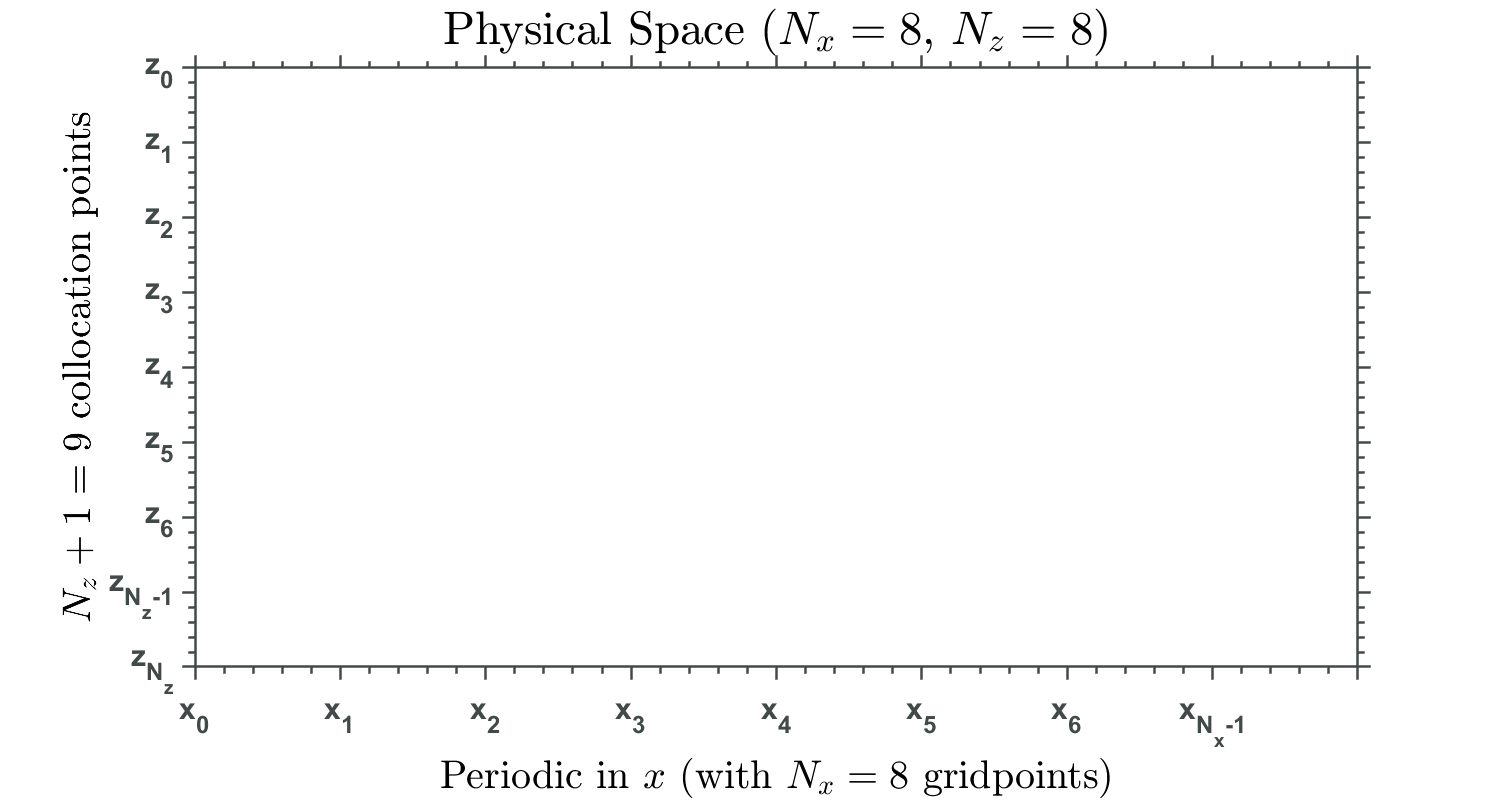
\includegraphics[width=16cm,height=16cm,keepaspectratio]{sections/other/matt_1.png}%
    \vspace{1mm}
    \caption{In Physical Space, we consider $N_x$ discretization points on the $x$--axis \\and $N_z+1$ collocation points on the $z$--axis.}%
    \label{fig:physical_space}%
\end{figure}


\vspace{-18mm}
\begin{figure}[H]
    \centering
    %\hspace{-15mm}
    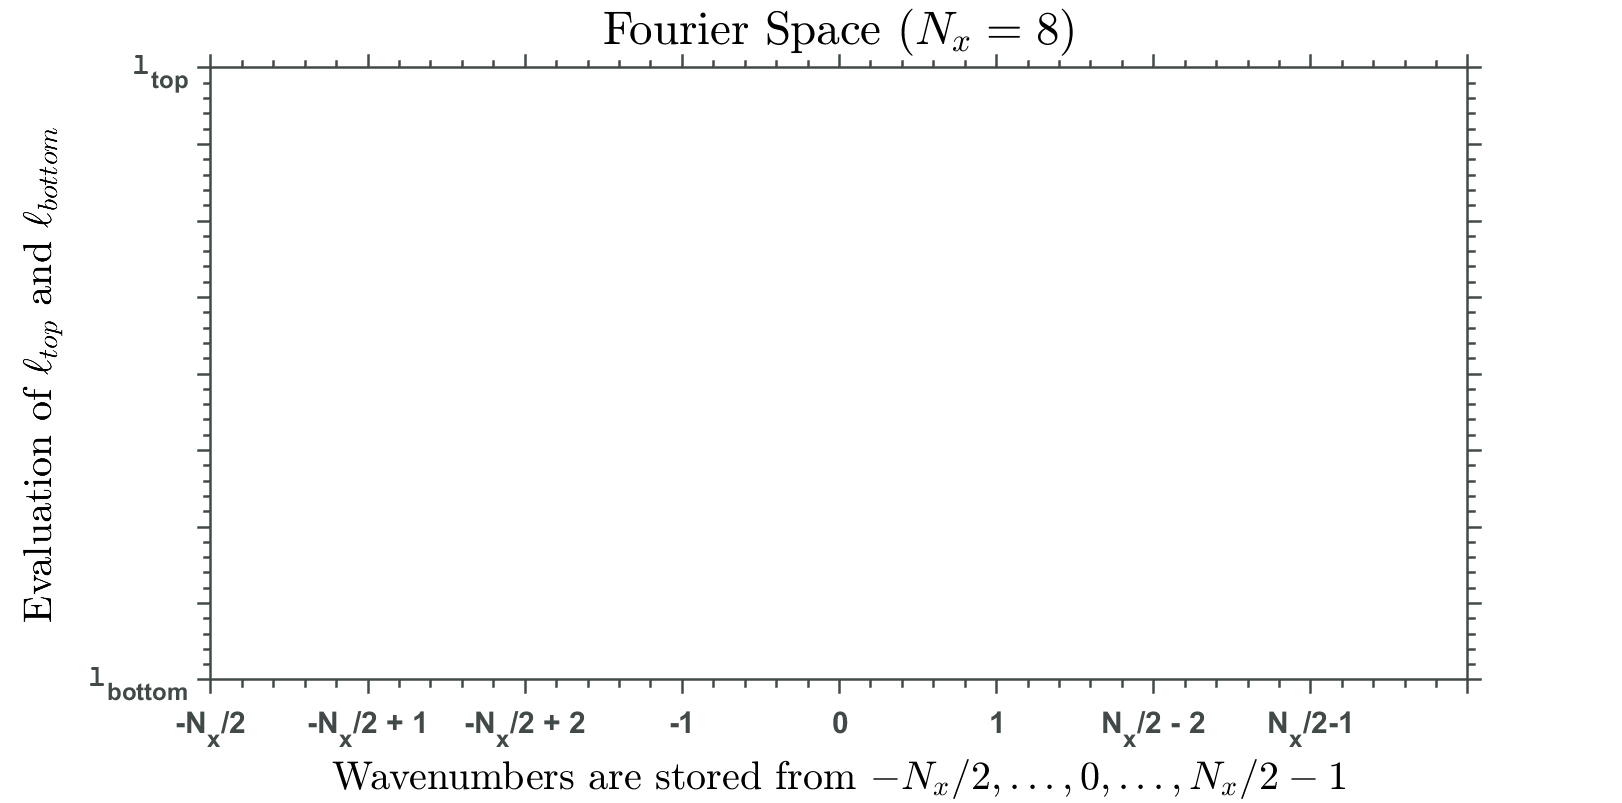
\includegraphics[width=16cm,height=16cm,keepaspectratio]{sections/other/matt_2.png}%
    \vspace{3mm}
    \caption{In Fourier Space, wavenumbers are stored in the order $-N_x/2,$ $\ldots,0,\ldots,N_x/2-1$ and $\ell_{top}$ and $\ell_{bottom}$ are evaluated at the upper boundary $z=a$ and the surface $z=0$ (cf. Algorithm $\text{A}.0.2$ and $\text{A}.0.3$).}
    \label{fig:fourier_space}%
\end{figure}
\vspace{-15mm}
More generally, we consider the Fourier transform on the $N_x$--point grid with a period of $d$. For $N_x$ discretization points and a step size of $(d/N_x)$, we have
\begin{align*}
\text{Physical ~Space :}&~~x\in\Big\{0,\
\frac{d}{Nx},\frac{2d}{Nx},\ldots,\frac{(N_x-2)d}{N_x},\frac{(N_x-1)d}{N_x}\Big\}   \\
\text{Fourier ~Space :}& ~~p\in\Big\{-\frac{N_x}{2},-\frac{N_x}{2}+1,\ldots,\frac{N_x}{2}-2,\frac{N_x}{2}-1\Big\}
\end{align*}
where the \gls{dft} is computed through several applications of the Fast Fourier Transform (FFT).
\chapter{Proof of Algebra Property, Elliptic Estimate, and Translation Property}
\label{Appendix B: Alebra and Elliptic Property}
\thispagestyle{pageonbottom}

\pagestyle{fancy}
\renewcommand{\sectionmark}[1]{\markright{#1}}
\fancyhead{}
%%%%%%%%%%%%%%%%%%%%%%%%%%%% The paper headers
\fancyhead[LE,RO]{\thepage}
\fancyhead[LO]{\text{Appendix B} \quad   {Algebra Property and Elliptic Estimate}}
\fancyhead[RE]{\text{Appendix B} \quad   {Algebra Property and Elliptic Estimate}} %Even page header and number at left top
\fancyfoot[L,R,C]{}
\renewcommand{\headrulewidth}{1pt}% disable the underline of the header part

As discussed in $\S 2.7$, we present the proof of the three major tools used to show joint analyticity of the upper field in the appropriate Sobolev space. Our first property is the ``Algebra Property" for estimating products of functions, the second property is a rigorous statement of the ``Elliptic Estimate," and our final property shows how to bound translated elements in our function spaces. The same techniques will work for the lower field in $\S3.6$ where the interval $[0,a]$ is translated to $[-b,0]$.
\begin{lemma}[{Algebra Property}] Given an integer $s \ge 0$ and any $\sigma > 0$, there exists a constant $\mathcal{M}=\mathcal{M}(s)$ such that if $f\in C^s([0,d]),u\in H^s([0,d]\times [0,a])$ then
\begin{equation}
\|fu\|_{H^s} \le \mathcal{M}|f|_{C^s}\|u\|_{H^s},
\end{equation}
and if $\tilde{f}\in C^{s+1/2+\sigma}([0,d]),\tilde{u}\in H^{s+1/2}([0,d])$ then there exists a constant $\tilde{\mathcal{M}}=\tilde{\mathcal{M}}(s)$ such that
\begin{equation}
 \|\tilde{f}\tilde{u}\|_{H^{s+1/2}} \le \tilde{\mathcal{M}}|\tilde{f}|_{C^{s+1/2+\sigma}}\|\tilde{u}\|_{H^{s+1/2}}.   
\end{equation}
\end{lemma}
\vspace{1 mm}
\begin{proof}{[Lemma B.0.1]} Let $s\in \mathbb N_0:=\mathbb N\cup\{0\}, f\in C^s([0,d])$, and $u\in H^s([0,d]\times [0,a])$. We will first verify $(\text{B}.1)$. For this, the definition of our Sobolev norms and Leibniz's formula delivers
\begin{align*}
\|fu\|_{H^s}^2 &= \sum_{\ell=0}^s \sum_{m=0}^{\ell} \norm{\partial_z^{s-\ell}\partial_x^{\ell - m}(fu)}_{L^2}^2 \\&=
\sum_{\ell=0}^s \sum_{m=0}^{\ell}\norm{ \sum_{p=0}^{s-\ell}\sum_{q=0}^{\ell-m}\binom{s - \ell}{p}\binom{\ell - m}{q}\left[\partial_z^{s-\ell-p}\partial_x^{\ell-m-q}f\right]\Big[\partial_z^p\partial_x^{q}u\Big]}_{L^2}^2
\end{align*}
As $f\in C^s([0,d])$ only depends on the $x$--component, the expression inside the norm is zero unless $s-\ell= p$ and we deduce
\bes
\sum_{p=0}^{s-\ell}\sum_{q=0}^{\ell-m}\binom{s - \ell}{p}\binom{\ell - m}{q}\left[\partial_z^{s-\ell-p}\partial_x^{\ell-m-q}f\right]\Big[\partial_z^p\partial_x^{q}u\Big]=\sum_{q=0}^{\ell-m}\binom{\ell - m}{q}\left[\partial_x^{\ell-m-q}f\right]\left[\partial_z^{s-\ell}\partial_x^{q}u\right].
\ees
Therefore
\begin{align}
\|fu\|_{H^s}^2 &= \sum_{\ell=0}^s \sum_{m=0}^{\ell}\norm{\sum_{q=0}^{\ell-m}\binom{\ell - m}{q}\left[\partial_x^{\ell-m-q}f\right]\left[\partial_z^{s-\ell}\partial_x^{q}u\right]}_{L^2}^2 \nonumber\\&\leq 
\sum_{\ell=0}^s \sum_{m=0}^{\ell}\sum_{q=0}^{\ell-m}\binom{\ell - m}{q}\left|\partial_x^{\ell-m-q}f\right|_{L^{\infty}}^2 \norm{\partial_z^{s-\ell}\partial_x^{q}u}_{L^2}^2 \nonumber\\& \leq
\sum_{\ell=0}^s \sum_{m=0}^{\ell}\sum_{q=0}^{\ell-m}\binom{\ell - m}{q} \left|f\right|_{C^s}^2 \norm{u}_{H^s}^2.
\end{align}
By the binomial theorem we may observe
\bes
\sum_{q=0}^{\ell-m}\binom{\ell - m}{q}= 2^{\ell-m}.
\ees
Inserting the above expression into $(\text{B}.3)$ and repeatedly applying the definition of the geometric series gives
\begin{align*}
\|fu\|_{H^s}^2 & \leq 
\sum_{\ell=0}^s \sum_{m=0}^{\ell} 2^{\ell-m}\left|f\right|_{C^s}^2 \norm{u}_{H^s}^2 \\&=
\sum_{\ell=0}^s 2^{\ell} \sum_{m=0}^{\ell} 2^{-m}\left|f\right|_{C^s}^2 \norm{u}_{H^s}^2 \\& =
\sum_{\ell=0}^s 2^{\ell}\left(2-2^{-m}\right)\left|f\right|_{C^s}^2 \norm{u}_{H^s}^2\\&\leq
\sum_{\ell=0}^s 2^{\ell+1}\left|f\right|_{C^s}^2 \norm{u}_{H^s}^2 \\&=
\left(2^{s+2}-2\right)\left|f\right|_{C^s}^2 \norm{u}_{H^s}^2,
\end{align*}
and the inequality $(\text{B}.1)$ follows by taking the square root.

Next, we follow \cite{NichollsReitich99} to verify $(\text{B}.2)$. Suppose $s=\rho$ for $0<\rho < 1$ and $\Omega\subseteq \mathbb R^n$. Then a norm in $H^{\rho}(\Omega)$ that is equivalent to the usual Sobolev space norm is defined as
\begin{equation}
\|\tilde{u}\|_{H^{\rho}}^2 := \|\tilde{u}\|_{L^2}^2 +
\int_{\Omega} \int_{\Omega}\frac{|\tilde{u}(x)-\tilde{u}(z)|^2}{|e^{ix}-e^{iz}|^{2\rho + n}}\diff x \diff z.
\end{equation}
The above definition is a fractional order Sobolev space known as the Sobolev--Slobodeckij space. To establish $(\text{B}.2)$ we start with the case $s=0$ and evaluate $(\text{B}.4)$ with $\rho = 1/2$ 
\vspace{-3mm}
\begin{align}
\begin{split}
 \|\tilde{f}\tilde{u}\|_{H^{1/2}}^2 &= \|\tilde{f}\tilde{u}\|_{L^2}^2 + \int_{\Omega} \int_{\Omega}\frac{|\tilde{f}(x)\tilde{u}(x)-\tilde{f}(z)\tilde{u}(z)|^2}{|e^{ix}-e^{iz}|^{n+1}}\diff x \diff z\\& \le
|\tilde{f}|_{L^{\infty}}^2\|\tilde{u}\|_{L^2}^2 +
2\int_{\Omega} \int_{\Omega} \frac{|\tilde{f}(x)-\tilde{f}(z)|^2}{|e^{ix}-e^{iz}|^{n+1}}|\tilde{u}(x)|^2\diff x \diff z \\&\qquad+
2\int_{\Omega} \int_{\Omega}|\tilde{f}(z)|^2 \frac{|\tilde{u}(x)-\tilde{u}(z)|^2}{|e^{ix}-e^{iz}|^{n+1}}\diff x \diff z,
\end{split}
\end{align}
where it is clear that the first and third terms in $(\text{B}.5)$ can be grouped together and bounded 
\bes
|\tilde{f}|_{L^{\infty}}^2\|\tilde{u}\|_{L^2}^2 + 2\int_{\Omega} \int_{\Omega}|\tilde{f}(z)|^2 \frac{|\tilde{u}(x)-\tilde{u}(z)|^2}{|e^{ix}-e^{iz}|^{n+1}}\diff x \diff z \leq C|\tilde{f}|_{L^{\infty}}^2\|\tilde{u}\|_{H^{1/2}}^2.
\ees
To bound the second term in $(\text{B}.5)$ we observe
\begin{align}
\begin{split}
2\int_{\Omega} \int_{\Omega} &\frac{|\tilde{f}(x)-\tilde{f}(z)|^2}{|e^{ix}-e^{iz}|^{n+1}}|\tilde{u}(x)|^2\diff x \diff z \\&\le 2
|\tilde{f}|_{C^{1/2+\sigma}}^2 \int_{\Omega} \int_{\Omega}
\frac{|x-z|^{1+2\sigma}}{|e^{ix}-e^{iz}|^{n+1}}|\tilde{u}(x)|^2\diff x \diff z \\&\le
C|\tilde{f}|_{C^{1/2+\sigma}}^2 \|\tilde{u}\|_{L^2}^2,
\end{split}
\end{align}
so that $(\text{B}.5)$ and $(\text{B}.6)$ establish the inequality $(\text{B}.2)$ in the case $s=0$
$$ \|\tilde{f}\tilde{u}\|_{H^{1/2}} \leq  \tilde{\mathcal{M}}(s)|\tilde{f}|_{C^{1/2+\sigma}}\|\tilde{u}\|_{H^{1/2}}.$$
In general, for $s>0$ we have
\begin{equation}
\|\tilde{u}\|_{H^{s+1/2}}^2 = \|\tilde{u}\|_{H^s}^2 + \|\partial_x^s \tilde{u}\|_{H^{1/2}}^2,
\end{equation}
and from $(\text{B}.1)$
\begin{equation}
\|\tilde{f}\tilde{u}\|_{H^s} \le \tilde{\mathcal{M}}(s)|\tilde{f}|_{C^s}\|\tilde{u}\|_{H^s}.
\end{equation}
For $s>0$, the regularity of $\tilde{f}\in C^{s+1/2+\sigma}(\Omega)$ and the estimates $(\text{B}.5)$ and $(\text{B}.6)$ imply
\begin{equation}
\|\partial_x^s (\tilde{f}\tilde{u})\|_{H^{1/2}} \le 
\tilde{\mathcal{M}}(s)|\tilde{f}|_{C^{s+1/2+\sigma}}\|\tilde{u}\|_{H^{s+1/2}}.
\end{equation}
Finally, the equation $(\text{B}.7)$ and estimates $(\text{B}.8)$ and $(\text{B}.9)$ deliver 
$$
\|\tilde{f}\tilde{u}\|_{H^{s+1/2}}^2 = \|\tilde{f}\tilde{u}\|_{H^s}^2 + \|\partial_x^s (\tilde{f}\tilde{u})\|_{H^{1/2}}^2\leq \tilde{\mathcal{M}}(s)|\tilde{f}|_{C^{s+1/2+\sigma}}^2\|\tilde{u}\|_{H^{s+1/2}}^2,$$
which is the required estimate for $s>0$. 
\end{proof}


\vskip 0.1in
\begin{theorem}[{Elliptic Estimate}] Given an integer $s\ge 0$, if $F\in H^s([0,d])\times [0,a]),$ $\zeta^u \in H^{s+3/2}([0,d]),$ $P\in H^{s+1/2}([0,d])$, then there exists a unique solution $u\in H^{s+2}([0,d])\times [0,a])$ of
\begin{subequations}
\begin{align}
\Delta u(x,z) +2i\underline{\alpha}\partial_{x}u(x,z)+(\underline{\gamma}^u)^2u(x,z)&=F(x,z), && \text{$0<z<a$},\\
u(x,0)&=\zeta^u(x,0), && \text{at $z=0$},\\
u(x+d,z)&=u(x,z),\\
\partial_z u(x,a)-T_0^u[u(x,a)] &= P(x), && \text{at $z=a$},
\end{align}
\end{subequations}
satisfying 
\begin{equation}\|u\|_{H^{s+2}}\le C_e\{\|F\|_{H^{s}}+\|\zeta^u\|_{H^{s+3/2}}+\|P\|_{H^{s+1/2}}  \}, \end{equation}
for some constant $C_e = C_e(s) > 0$.
\end{theorem}
\vspace{1 mm}
\begin{proof}{[Lemma B.0.2]} Following \cite{HongNicholls20}, we let $\tilde{\zeta}^u=[-\partial_zu]_{z=0}$ where we define the DNO
\bes
G:(\zeta^u,P,F)\to \tilde{\zeta}^u, \quad G[\zeta^u,P,F]=G^{(0)}[\zeta^u] + G^{(a)}[P] + G^{([0,a])}[F].
\ees
With these, we will obtain the estimates
\begin{subequations}
\begin{align}
\norm{G^{(0)}[\zeta^u]}_{H^{s+1/2}}&\leq C_{G^{(0)}}\norm{\zeta^u}_{H^{s+3/2}},\\
\norm{G^{(a)}[P]}_{H^{s+1/2}}&\leq C_{G^{(a)}}\norm{P}_{H^{s+1/2}},\\
\norm{G^{([0,a])}[F]}_{H^{s+1/2}}&\leq C_{G^{([0,a])}}\norm{F}_{H^{s}}.
\end{align}
\end{subequations}
As in $\S 2.11$, we posit the expansions
\bes
\{u,F\}(x,z)=\sum_{p=-\infty}^{\infty}\{\hat{u}_{p},\hat{F}_p\}(z)e^{i\tilde{p} x},\quad \{\zeta^u,P\}(x)=\sum_{p=-\infty}^{\infty}\{\hat{\zeta}_p^u,\hat{P}_{p}\}e^{i\tilde{p} x},
\ees
into $(\text{B}.10)$ which delivers the two--point boundary value problem
\begin{align*}
\partial_z^2\hat{u}_{p}(z)+\left((\underline{\gamma}_p^u)^2-\tilde{p}^2-2\underline{\alpha}\tilde{p}\right)\hat{u}_{p}(z)&=\hat{F}_{p}(z),&&\text{$0<z<a$},\\
\hat{u}_{p}(0)&=\hat{\zeta}_{p}^u,&& \text{at $z=0$},\\
\partial_z \left[\hat{u}_{p}(a)\right] - (i\ugamma_p^u)[\hat{u}_{p}(a)]&=\hat{P}_{p},&& \text{at $z=a$},
\end{align*}
where
\bes
\ugamma_p^u = \begin{cases} 
      (\ugamma_p^u)':=\sqrt{(\uk^u)^2-\ualpha_p^2},  & \ualpha_p^2 < (\uk^u)^2, \\
      0, & \ualpha_p^2 = (\uk^u)^2, \\
      i(\ugamma_p^u)'':=i\sqrt{\ualpha_p^2-(\uk^u)^2}, & \ualpha_p^2 > (\uk^u)^2,
   \end{cases} \quad (\ugamma_p^u)',(\ugamma_p^u)''\in\mathbb R,\quad (\ugamma_p^u)',(\ugamma_p^u)''>0.
\ees
The primed notation denotes $'$ as the real part and $''$ as the imaginary part. 
Observing
\begin{align*}
(\ugamma_p^u)^2-\tilde{p}^2-2\ualpha\tilde{p}&=
\ualpha^2 + (\ugamma_p^u)^2 - (\ualpha+\tilde{p})^2 := 
(\uk^u)^2 - \ualpha_p^2 = (\ugamma_p^u)^2,
\end{align*}
delivers

\begin{align*}
\partial_z^2\hat{u}_{p}(z)+(\underline{\gamma}_p^u)^2\hat{u}_{p}(z)&=\hat{F}_{p}(z),&&\text{$0<z<a$},\\
\hat{u}_{p}(0)&=\hat{\zeta}_{p}^u,&& \text{at $z=0$},\\
\partial_z \left[\hat{u}_{p}(a)\right] - (i\ugamma_p^u)[\hat{u}_{p}(a)]&=\hat{P}_{p},&& \text{at $z=a$}.
\end{align*}
We now consider a function $\Phi_0(z;p)$ satisfying
\begin{align*}
\partial_z^2\Phi_0(z;p)+(\underline{\gamma}_p^u)^2\Phi_0(z;p)&=0,&&\text{$0<z<a$},\\
\Phi_0(0;p)&=1,&& \text{at $z=0$},\\
\partial_z \Phi_0(a;p) - (i\ugamma_p^u)\Phi_0(a;p)&=0,&& \text{at $z=a$},
\end{align*}
so that the solution of
\begin{align*}
\partial_z^2\hat{u}_{p}(z)+(\underline{\gamma}_p^u)^2\hat{u}_{p}(z)&=0,&&\text{$0<z<a$},\\
\hat{u}_{p}(0)&=\hat{\zeta}_{p}^u,&& \text{at $z=0$},\\
\partial_z \left[\hat{u}_{p}(a)\right] - (i\ugamma_p^u)[\hat{u}_{p}(a)]&=0,&& \text{at $z=a$},
\end{align*}
is 
\bes
\hat{u}_p(z) = \hat{\zeta}_{p}^u\Phi_0(z;p).
\ees
Similarly, we consider a function $\Phi_a(z;p)$ satisfying
\begin{align*}
\partial_z^2\Phi_a(z;p)+(\underline{\gamma}_p^u)^2\Phi_a(z;p)&=0,&&\text{$0<z<a$},\\
\Phi_a(0;p)&=0,&& \text{at $z=0$},\\
\partial_z \Phi_a(a;p) - (i\ugamma_p^u)\Phi_a(a;p)&=1,&& \text{at $z=a$},
\end{align*}
so that the solution of
\begin{align*}
\partial_z^2\hat{u}_{p}(z)+(\underline{\gamma}_p^u)^2\hat{u}_{p}(z)&=0,&&\text{$0<z<a$},\\
\hat{u}_{p}(0)&=0,&& \text{at $z=0$},\\
\partial_z \left[\hat{u}_{p}(a)\right] - (i\ugamma_p^u)[\hat{u}_{p}(a)]&=\hat{P}_{p},&& \text{at $z=a$},
\end{align*}
is 
\bes
\hat{u}_p(z) = \hat{P}_{p}\Phi_a(z;p).
\ees
With these, the unique solution of the two--point boundary value problem is given by
\be
\hat{u}_p(z)=\hat{\zeta}_p^u\Phi_0(z;p)+\hat{P}_pe^{i\ugamma_p^ua}\Phi_a(z;p) - I_0[\hat{F}_p](z) - I_a[\hat{F}_p](z),
\ee
where one can readily verify that
\bes
\Phi_0(z;p)=e^{i\ugamma_p^uz}:= \begin{cases} 
      e^{i(\ugamma_p^u)'z}, & \ualpha_p^2 < (\uk^u)^2, \\
      1, & \ualpha_p^2 = (\uk^u)^2, \\
      e^{-(\ugamma_p^u)''z}, & \ualpha_p^2 > (\uk^u)^2,
   \end{cases}
\ees
and
\bes
\Phi_a(z;p)=\frac{\sinh(\ugamma_p^uz)}{\ugamma_p^u}:= \begin{cases} 
      \frac{\sin\left((\ugamma_p^u)'z\right)}{(\ugamma_p^u)'}, & \ualpha_p^2 < (\uk^u)^2, \\
      z, & \ualpha_p^2 = (\uk^u)^2, \\
      \frac{\sinh\left((\ugamma_p^u)''z\right)}{(\ugamma_p^u)''}, & \ualpha_p^2 > (\uk^u)^2,
   \end{cases}
\ees
and
\begin{align*}
I_0[\hat{F}_p](z)&:=\int_0^z \Phi_0(z;p) \Phi_a(s;p) \hat{F}_p(s)\diff s,\\
I_a[\hat{F}_p](z)&:=\int_z^a \Phi_0(s;p) \Phi_a(z;p) \hat{F}_p(s)\diff s.
\end{align*}
By the Leibniz integral rule
\begin{align*}
\partial_zI_0[\hat{F}_p](z)&=\Phi_0(z;p) \Phi_a(z;p) \hat{F}_p(z) + \int_0^z \left(\partial_z\Phi_0(z;p)\right) \Phi_a(s;p) \hat{F}_p(s)\diff s,\\
\partial_zI_a[\hat{F}_p](z)&=-\Phi_0(z;p) \Phi_a(z;p) \hat{F}_p(z) + \int_z^a \Phi_0(s;p) \left(\partial_z\Phi_a(z;p)\right) \hat{F}_p(s)\diff s.
\end{align*}
Adding the two expressions above and substituting the result into $(\text{B}.13)$ gives
\be
\partial_z\hat{u}_p(z)=\hat{\zeta}_p^u\partial_z\Phi_0(z;p)+\hat{P}_pe^{i\ugamma_p^ua}\partial_z\Phi_a(z;p) - \tilde{I}_0[\hat{F}_p](z) - \tilde{I}_a[\hat{F}_p](z),
\ee
where
\begin{align*}
\tilde{I}_0[\hat{F}_p](z)&:=\int_0^z \left(\partial_z\Phi_0(z;p)\right) \Phi_a(s;p) \hat{F}_p(s)\diff s,\\
\tilde{I}_a[\hat{F}_p](z)&:=\int_z^a \Phi_0(s;p) \left(\partial_z\Phi_a(z;p)\right) \hat{F}_p(s)\diff s.
\end{align*}
Evaluating $(\text{B.14})$ at $z=0$ and multiplying by negative one yields
\begin{align*}
-\partial_z\hat{u}_p(0)&=-\hat{\zeta}_p^u\partial_z\Phi_0(0;p)-\hat{P}_pe^{i\ugamma_p^ua}\partial_z\Phi_a(0;p) + \tilde{I}_0[\hat{F}_p](0) + \tilde{I}_a[\hat{F}_p](0)\\&=
-\hat{\zeta}_p^u(i\ugamma_p^u) - \hat{P}_pe^{i\ugamma_p^ua} + \int_0^a e^{i\ugamma_p^us} \hat{F}_p(s)\diff s.
\end{align*}
From this, we deduce
\bes
G^{(0)}[\zeta^u] = - \sump \big[\partial_z\Phi_0(0;p)\big] \hat{\zeta}_p^ue^{i\tilde{p}x} = \sump (-i\ugamma_p^u)\hat{\zeta}_p^ue^{i\tilde{p}x},
\ees
and
\bes
G^{(a)}[P] = - \sump \big[e^{i\ugamma_p^u a}\partial_z\Phi_a(0;p)\big] \hat{P}_pe^{i\tilde{p}x} = \sump (-e^{i\ugamma_p^u a})\hat{P}_pe^{i\tilde{p}x},
\ees
and
\bes
G^{([0,a])}[F] = \sump \int_0^a \left(e^{i\ugamma_p^u s}\hat{F}_p(s)\diff s\right)e^{i\tilde{p}x}.
\ees
With these, we use our Sobolev norms in $\S 2.7$ and follow the proof of Lemma $2.8.2$ to estimate
\begin{align*}
\norm{G^{(0)}[\zeta^u]}_{H^{s+1/2}}^2&=\sum_{p=-\infty}^{\infty}\left|(i\ugamma_p^u)\hat{\zeta}_p^u\right|^2\langle \tilde{p} \rangle^{2(s+1/2)} \\& \leq
C_{G^{(0)}}\sum_{p=-\infty}^{\infty}\left|\hat{\zeta}_p^u\right|^2\langle \tilde{p} \rangle^{2(s+3/2)} \\&=
C_{G^{(0)}}\norm{\zeta^u}_{H^{s+3/2}}^2.
\end{align*}
and
\begin{align*}
\norm{G^{(a)}[P]}_{H^{s+1/2}}^2&= \sum_{p=-\infty}^{\infty}\left|\left(e^{i\ugamma_p^u a}\right)\hat{P}_p\right|^2\langle \tilde{p} \rangle^{2(s+1/2)} \\&\leq
C_{G^{(a)}}\sum_{p=-\infty}^{\infty}\left|\hat{P}_p\right|^2\langle \tilde{p} \rangle^{2(s+1/2)} \\&=
C_{G^{(a)}}\norm{P}_{H^{s+1/2}}^2.
\end{align*}
We then apply the Cauchy--Schwarz inequality to estimate
\begin{align*}
\norm{G^{([0,a])}[F]}_{H^{s+1/2}}^2&= \sum_{p=-\infty}^{\infty}\left|\int_0^a e^{i\ugamma_p^u s}\hat{F}_p(s)\diff s\right|^2\langle \tilde{p} \rangle^{2(s+1/2)}  \\&\leq
\sum_{p=-\infty}^{\infty}\int_0^a \left|e^{i\ugamma_p^u s}\right|^2\diff s \int_0^a \left| \hat{F}_p(s)\right|^2\diff s~\langle \tilde{p} \rangle^{2(s+1/2)}.
\end{align*}
By the definition of $\Phi_0(s;p)$ the middle term becomes
\bes
\int_0^a \left|e^{i\ugamma_p^u s}\right|^2\diff s =\begin{cases} 
      a, & \ualpha_p^2 < (\uk^u)^2, \\
      a, & \ualpha_p^2 = (\uk^u)^2, \\
     \int_0^a e^{-2(\ugamma_p^u)''s}\diff s , & \ualpha_p^2 > (\uk^u)^2,
   \end{cases}
\ees
where

\bes
\int_0^a e^{-2(\ugamma_p^u)''s} \diff s =\frac{1}{2(\ugamma_p^u)''}\left(1-e^{-2(\ugamma_p^u)''a}\right)\leq \frac{1}{2(\ugamma_p^u)''}.
\ees
By defining for $q\in\{u,w\}$
\be
\mathcal{\uU}^q:=\{p\in\mathbb Z ~|~ \ualpha_p^2 \leq (\uk^q)^2\},\quad
\ugamma_p^q:= \begin{cases} 
      \sqrt{(\uk^q)^2-\ualpha_p^2}, & p\in\mathcal{\uU}^q, \\
      i\sqrt{\ualpha_p^2-(\uk^q)^2}, & p\not\in\mathcal{\uU}^q,
   \end{cases}
\ee
the third estimate follows from the bounds
\begin{align*}
\norm{G^{([0,a])}[F]}_{H^{s+1/2}}^2 &\leq \sum_{p=-\infty}^{\infty}\int_0^a \left|e^{i\ugamma_p^u s}\right|^2\diff s \int_0^a \left| \hat{F}_p(s)\right|^2\diff s~\langle \tilde{p} \rangle^{2(s+1/2)} \\& \leq
\sum_{p\in \mathcal{\uU}^u} a\langle \tilde{p} \rangle^{2(s+1/2)} \Norm{\hat{F}_p}{L^2([0,a])}^2 + \sum_{p\not\in \mathcal{\uU}^u}\frac{\langle \tilde{p} \rangle^{2(s+1/2)}}{2(\ugamma_p^u)''}\Norm{\hat{F}_p}{L^2([0,a])}^2
\\& \leq
C\sum_{p\in \mathcal{\uU}^u}\langle \tilde{p} \rangle^{2s}\Norm{\hat{F}_p}{L^2([0,a])}^2 + \tilde{C}\sum_{p\not\in \mathcal{\uU}^u}\langle \tilde{p} \rangle^{2s}\Norm{\hat{F}_p}{L^2([0,a])}^2 \\&\leq
C_{G^{([0,a])}}\sum_{p=-\infty}^{\infty}\langle\tilde{p} \rangle^{2s}\Norm{\hat{F}_p}{L^2([0,a])}^2, \quad C_{G^{([0,a])}}=\max\left\{a\langle\tilde{p} \rangle,1/2\right\}
\\&= C_{G^{([0,a])}}\norm{F}_{H^{s}}^2,
\end{align*}
which validates $(\text{B}.12)$. These imply
\bes
\|u\|_{H^{s+2}}\le C_e\{\|F\|_{H^{s}}+\|\zeta^u\|_{H^{s+3/2}}+\|P\|_{H^{s+1/2}}  \},
\ees
where
\bes
C_e := \max\big\{C_{G^{(0)}},C_{G^{(a)}}, C_{G^{([0,a])}}\big\}.
\ees
\end{proof}


\vskip 0.1in
\begin{lemma}[{Translation Property}]
Given an integer $s\ge 0$, if $F\in H^s([0,d])\times [0,a])$, then $(a-z)F \in$ $H^s([0,d])\times [0,a])$ and there exists a positive constant $Z_a = Z_a(s)$ such that
$$\|(a-z)F\|_{H^s} \le Z_a \|F\|_{H^s}.$$
\end{lemma}
\vskip 0.1in
\begin{proof}{[Lemma B.0.3]}
As $(a-z)$ is a constant, it is clear that $(a-z)F \in$ $H^s([0,d])\times [0,a])$. The required estimate then follows from applying Lemma $\text{B}.0.1$.

\end{proof}
\chapter{Change of Variables}
\label{Appendix C: Change of Variables}
\thispagestyle{pageonbottom}

\pagestyle{fancy}
\renewcommand{\sectionmark}[1]{\markright{#1}}
\fancyhead{}
%%%%%%%%%%%%%%%%%%%%%%%%%%%% The paper headers
\fancyhead[LE,RO]{\thepage}
\fancyhead[LO]{\text{Appendix C} \quad   {Change of Variables}}
\fancyhead[RE]{\text{Appendix C} \quad   {Change of Variables}} %Even page header and number at left top
\fancyfoot[L,R,C]{}
\renewcommand{\headrulewidth}{1pt}% disable the underline of the header part

This appendix covers a fundamental step in our Boundary Perturbation algorithm. One of the primary objectives in Chapters $2$ and $3$ is to show that both the upper/lower fields and the upper/lower layer DNOs are analytic with respect to two small perturbation parameters. In order to do this, we perform a domain--flattening change of variables (known as $\sigma$--coordinates in oceanography \cite{Phillips57} and the C--method in the dynamical theory of gratings \cite{CDCM82,CMR80}). We will present the theory in Cartesian coordinates and will later state the effects on the Helmholtz equation and the overall impact on our governing equations. The bulk of our analysis is based on Appendix E in \cite{HOPS_Notes}.
\vspace{3mm}
\begin{flushleft}
We begin by considering the doubly--perturbed domain
\end{flushleft}
\begin{equation}
S_{L,U}:=\{L(x)<z<U(x)\}=\{\overline{\ell}+\ell(x)<z<\overline{u}+u(x)\},    
\end{equation}
where the change of variables 
\begin{equation}
    x'=x,\quad z'=\overline{\ell}\left(\frac{U-z}{U-L}\right)+\overline{u}\left(\frac{z-L}{U-L}\right),
\end{equation}
maps $S_{L,U}$ to $S_{\overline{\ell},\overline{u}}$. As discussed in Chapter $1$, the variables $u$ and $U$ both refer to the upper boundary while $\ell$ and $L$ reference the lower boundary. In the upper layer, the upper boundary is the artificial boundary at $\{z=a\}$ while the lower boundary is the surface $z=g(x)$. In the lower layer, the upper boundary is the surface $z=g(x)$ and the lower boundary is the artificial boundary at $\{z=-b\}$.  Defining the height of the layer to be
$$\overline{h}:=\overline{u}-\overline{\ell},$$
and using the formulas for $L$ and $U$, we find

$$\left(1+\frac{u(x)-\ell(x)}{\overline{h}}\right)z'= z-\left(\frac{\overline{u}\ell(x)-\overline{\ell}u(x)}{\overline{h}}\right), $$
or
$$C(x)z'=z-D(x),$$
where
\be
C(x):=1+\frac{u(x)-\ell(x)}{\overline{h}},\quad D(x):=\frac{\overline{u}\ell(x)-\overline{\ell} u(x)}{\overline{h}}.
\ee
In the upper layer we have
$$\overline{\ell}=0,\quad \ell=g, \quad \overline{u}=a, \quad u = 0,\quad \overline{h}=\overline{u}-\overline{\ell}=a.$$
Similarly, in the lower layer we have
$$\overline{\ell}=-b,\quad \ell=0, \quad \overline{u}=0, \quad u = g,\quad \overline{h}=\overline{u}-\overline{\ell}=b.$$
For a function $v=v(x,z)$, $v\in\{u,w\}$, which is transformed to
$$v'=v'(x',z')=v(x(x',z'),z(x',z')), \quad v=v(x,z)=v'(x'(x,z),z'(x,z)),$$
and $v'\in \{u',w'\},$ we apply the chain rule
$$\frac{\partial v}{\partial x}=\frac{\partial v'}{\partial x'}\frac{\partial x'}{\partial x}+\frac{\partial v'}{\partial z'}\frac{\partial z'}{\partial x},\quad  \frac{\partial v}{\partial z}=\frac{\partial v'}{\partial x'}\frac{\partial x'}{\partial z}+\frac{\partial v'}{\partial z'}\frac{\partial z'}{\partial z}.$$
Then
$$\frac{\partial x'}{\partial x}=1,\quad \frac{\partial x'}{\partial z}=0,\quad \frac{\partial z'}{\partial z}=\frac 1C,$$
where differentiating $Cz'=z-D$ with respect to $x$ yields
$$\left(\partial_x C\right)z'+C\left(\frac{\partial z'}{\partial x}\right)=-\left(\partial_x D\right),$$
and
$$\frac{\partial z'}{\partial x}=-\left(\frac{\left(\partial_x C\right)z'+\left(\partial_x D\right)}{C}\right)=-\frac EC.$$
We define
$$E(x,z'):=\left(\partial_x C\right)z'+\left(\partial_x D\right),$$
and observe that
$$\partial_x C=\frac{\partial_x u - \partial_x \ell}{\overline{h}},\quad \partial_x D=\frac{\overline{u}\partial_x \ell - \overline{\ell}\partial_x u}{\overline{h}}.   $$
This implies
\be
E=\frac{(\partial_x u - \partial_x \ell)z'+\overline{u}\partial_x \ell - \overline{\ell}\partial_x u}{\overline{h}}=(\partial_x u)Z_L + (\partial_x\ell)Z_U,
\ee
for the definitions
$$Z_L:=\frac{z'-\overline{\ell}}{\overline{h}},\quad Z_U:=\frac{\overline{u}-z'}{\overline{h}}.$$
We will later realize that it is more convenient to express our differentiation rules when premultiplied by $C$ (either $C(x)$ or $C(x')$ as appropriate) by which we settle upon the following differentiation rules under the change of variables in $(\text{C}.2)$
\be
C\partial_x = C\partial_{x'} - E\partial_{z'},\quad C\partial_z = \partial_{z'}.
\ee
\vspace{-10mm}
\begin{flushleft}In $\S 2.2$ and $\S 3.2$ we showed that the Helmholtz equation in the upper and lower layers can be represented by
\end{flushleft}
\vspace{-1mm}
\begin{equation}\Delta v +2i\alpha\partial_{x}v+(\gamma^v)^2 v=0.\end{equation}
We restate $(\text{C}.6)$ as
\begin{align*}0&=C^2\left\{\Delta v +2i\alpha\partial_{x}v+(\gamma^v)^2v\right\}\\&=
C^2\left\{\partial_{x}[\partial_{x} v]+ \partial_{z}[\partial_{z} v]+ +2i\alpha\partial_{x}v+(\gamma^v)^2v\right\}\\&=
C\partial_{x}[C\partial_{x} v]-C(\partial_{x} C)\partial_{x} v + C\partial_{z}[C\partial_{z} v] + 2C^2i\alpha\partial_{x}v+C^2(\gamma^v)^2v.
\end{align*}
By our transformation rules
\begin{align*}0&=
[C\partial_{x'}-E\partial_{z'}][C\partial_{x'}v' - E\partial_{z'}v']-(\partial_{x'}C)[C\partial_{x'}v' - E\partial_{z'}v']+\partial_{z'}[\partial_{z'}v'] + 2C^2i\alpha\partial_{x'}v'\\&~~~+C^2(\gamma^{v'})^2v'\\&=
C\partial_{x'}[C\partial_{x'}v']-E\partial_{z'}[C\partial_{x'}v']-C\partial_{x'}[E\partial_{z'}v']+E\partial_{z'}[E\partial_{z'}v']-(\partial_{x'}C)C\partial_{x'}v' \\&
~~~+(\partial_{x'}C)E\partial_{z'}v'+\partial_{z'}^2v'+2C^2i\alpha\partial_{x'}v'+C^2(\gamma^{v'})^2v'\\&=
\partial_{x'}[C^2\partial_{x'}v']-(\partial_{x'}C)C\partial_{x'}v'-\partial_{z'}[EC\partial_{x'}v']+(\partial_{z'}E)C\partial_{x'}v'-\partial_{x'}[CE\partial_{z'}v']\\&~~~+(\partial_{x'}C)E\partial_{z'}v'
+\partial_{z'}[E^2\partial_{z'}v']-(\partial_{z'}E)E\partial_{z'}v'-(\partial_{x'}C)C\partial_{x'}v' + (\partial_{x'}C)E\partial_{z'}v'\\&~~~+\partial_{z'}^2v'+2C^2i\alpha\partial_{x'}v'+C^2(\gamma^{v'})^2v',
\end{align*}
where
$$(\partial_{x'}C)E\partial_{z'}v' -(\partial_{z'}E)E\partial_{z'}v'-(\partial_{x'}C)C\partial_{x'}v' + (\partial_{x'}E)C\partial_{z'}v' = 0,$$ 
because
$$\partial_{z'}E=\partial_{x'}C=\partial_x C.$$
The second, forth, eight, and tenth terms cancel so that
\begin{align*}0=\partial_{x'}[C^2\partial_{x'}v']-\partial_{z'}[EC\partial_{x'}v']-\partial_{x'}[CE\partial_{z'}v']+(\partial_{x'}C)E\partial_{z'}v' \\+\partial_{z'}[E^2\partial_{z'}v']-(\partial_{x'}C)C\partial_{x'}v' +\partial_{z'}^2v'+2C^2i\alpha\partial_{x'}v'+C^2(\gamma^{v'})^2v'.\end{align*}
This may be written more compactly as
\begin{equation*}0=\text{div}'[A\nabla' v']+B\cdot \nabla' v' +2C^2i\alpha\partial_{x'}v'+C^2(\gamma^{v'})^2v',\end{equation*}
where for $S=C^2$
$$A=\begin{pmatrix}
    S & -EC\\
    -EC & 1+E^2
  \end{pmatrix}, ~~~~~
  B=(\partial_{x'}C)\begin{pmatrix}
    -C\\
    E
  \end{pmatrix}.
$$
By the definitions of $C$ and $E$, $(\text{C}.3)$ and $(\text{C}.4)$, we have 
\begin{align*}
S&=1 + \frac{2}{\overline{h}}u-\frac{2}{\overline{h}}\ell+\frac{1}{\overline{h}^2}u^2+\frac{1}{\overline{h}^2}\ell^2-\frac{2}{\overline{h}^2}\ell u,\allowdisplaybreaks\\
CE&=Z_L(\partial_x u)+Z_U(\partial_x \ell) + \frac{Z_L}{\overline{h}}u(\partial_x u)-\frac{Z_U}{\overline{h}}\ell(\partial_x \ell)-\frac{Z_L}{\overline{h}}\ell(\partial_x u)+\frac{Z_U}{\overline{h}}u(\partial_x \ell),\\
E^2&=Z_L^2(\partial_x u)^2 + Z_U^2(\partial_x \ell)^2 + 2Z_LZ_U(\partial_x \ell)(\partial_x u).
\end{align*}

If $\ell=\delta\tilde{\ell}$ and $u=\Eps\tilde{u}$ then
\begin{align*}
A&=A(\delta,\Eps)=A_{0,0}+A_{1,0}\delta +A_{0,1}\Eps + 
+A_{2,0}\delta^2 + A_{0,2}\Eps^2 + A_{1,1}\delta\Eps,\\
B&=B(\delta,\Eps)=B_{1,0}\delta +B_{0,1}\Eps + 
+B_{2,0}\delta^2 + B_{0,2}\Eps^2 + B_{1,1}\delta\Eps,\\
S&=S(\delta,\Eps)=S_{0,0}+S_{1,0}\delta +S_{0,1}\Eps + 
+S_{2,0}\delta^2 + S_{0,2}\Eps^2 + S_{1,1}\delta\Eps,
\end{align*}
where
\begin{align*}
A_{0,0}&=\begin{pmatrix}
    1 & 0\\
    0 & 1
  \end{pmatrix},\quad
A_{1,0}=\frac{1}{\overline{h}}
  \begin{pmatrix}
    -2\tilde{\ell} & -\overline{h}Z_U(\partial_x \tilde{\ell})\\
    -\overline{h}Z_U(\partial_x \tilde{\ell}) & 0
  \end{pmatrix},\\
A_{0,1}&=\frac{1}{\overline{h}}
  \begin{pmatrix}
    -2\tilde{u} & -\overline{h}Z_L(\partial_x \tilde{u})\\
    -\overline{h}Z_L(\partial_x \tilde{u}) & 0
  \end{pmatrix},\\
A_{2,0}&=\frac{1}{\overline{h}^2}
  \begin{pmatrix}
    \tilde{\ell}^2 & \overline{h}Z_U\tilde{\ell}(\partial_x \tilde{\ell})\\
    \overline{h}Z_U\tilde{\ell}(\partial_x \tilde{\ell}) & \overline{h}^2 Z_U^2(\partial_x \tilde{\ell})^2
  \end{pmatrix},\\
A_{0,2}&=\frac{1}{\overline{h}^2}
  \begin{pmatrix}
    \tilde{u}^2 & -\overline{h}Z_L\tilde{u}(\partial_x \tilde{u})\\
    -\overline{h}Z_L\tilde{u}(\partial_x \tilde{u}) & \overline{h}^2 Z_L^2(\partial_x \tilde{u})^2
  \end{pmatrix},\\
A_{1,1}&=\frac{1}{\overline{h}^2}
  \begin{pmatrix}
    -2\tilde{\ell}\tilde{u} & \overline{h}\left(Z_L\tilde{\ell}(\partial_x \tilde{u})-Z_U\tilde{u}(\partial_x \tilde{\ell})\right)\\
    \overline{h}\left(Z_L\tilde{\ell}(\partial_x \tilde{u})-Z_U\tilde{u}(\partial_x \tilde{\ell})\right) & 2\overline{h}^2 Z_U Z_L(\partial_x \tilde{\ell})(\partial_x \tilde{u})
  \end{pmatrix},
\end{align*}
and 
\begin{align*}
B_{1,0}&=
\frac{1}{\overline{h}}\begin{pmatrix} (\partial_x \tilde{\ell}) \\0\end{pmatrix},\quad
B_{0,1}=
\frac{1}{\overline{h}}\begin{pmatrix} -(\partial_x \tilde{u}) \\0\end{pmatrix},\\
B_{2,0}&=
\frac{1}{\overline{h}^2}\begin{pmatrix} -\tilde{\ell}(\partial_x \tilde{\ell}) \\
-\overline{h}Z_U(\partial_x \tilde{\ell})^2\end{pmatrix},\\
B_{0,2}&=
\frac{1}{\overline{h}^2}\begin{pmatrix} -\tilde{u}(\partial_x \tilde{u}) \\
\overline{h}Z_L(\partial_x \tilde{u})^2\end{pmatrix},\\
B_{1,1}&=
\frac{1}{\overline{h}^2}\begin{pmatrix} \tilde{u}(\partial_x \tilde{\ell}) + \tilde{\ell}(\partial_x \tilde{u}) \\
\overline{h}(Z_U-Z_L)(\partial_x \tilde{\ell})(\partial_x \tilde{u})\end{pmatrix},
\end{align*}
and
\begin{align*}
S_{0,0}&=1,\quad S_{1,0}=-\frac{2}{\overline{h}}\tilde{\ell},\quad S_{0,1}=\frac{2}{\overline{h}}\tilde{u},\\
S_{2,0}&=\frac{1}{\overline{h}^2}\tilde{\ell}^2,\quad S_{0,2}=\frac{1}{\overline{h}^2}\tilde{u}^2,\quad S_{1,1}=-\frac{2}{\overline{h}^2}\tilde{\ell}\tilde{u}.
\end{align*}
\clearpage
\chapter{Permissions for the Inclusion of Published Works}
\label{Appendix C: Permission of Works}
\thispagestyle{pageonbottom}


The proof of joint analyticity and computation of the Reflectivity Map, including the related algorithms
and numerical experiments, are submitted to two separate SIAM journals, which allows authors to
use their articles in their thesis. Their policy states “Figures or tables created by someone other than the author or borrowed from a previously published source, even those created by the author and published elsewhere, must carry an appropriate credit line at the end of the caption.” The full policy is available at
\href{https://epubs.siam.org/journal-authors}{\color{blue}https://epubs.siam.org/journal-authors}. Upon acceptance, the author will update the necessary chapters and give the appropriate credit to the respective journal.
%\end{flushleft}
%\end{singlespacing}

% No need to make any changes to this file below this line.
\newpage
\phantomsection
\bibformb
%\bibliography{thesis}
%\bibliography{nicholls}
% MSK 2/22/2022 - Is the default spacing 1?
\setstretch{1}
\bibliography{nicholls}
\newpage
\vita
\fakechapter{Vita}
\begin{singlespace}
    \begin{description}[labelwidth=4cm,leftmargin=4.2cm,itemsep=1em]

        % Your full name bere
        \item[NAME] Matthew Shawn Kehoe

        % Put any degrees you have, in the form of: Degree type, Degree Field, Institution, City, State, Year
        \item[EDUCATION] Ph.D., Applied Mathematics, University of Illinois Chicago, IL, 2022
        \newline
        \\
        M.S., Computational Mathematics, University of Michigan at Dearborn, MI, 2015
        \newline
        \\
        B.A., Economics, Oakland University, MI, 2010
        
        \item[EXPERIENCE] Graduate Research and Teaching Assistant, University of Illinois Chicago, 2018 -- 2022
        \newline
        \\
        NSF Mathematical Sciences Graduate Intern, Cold Regions Research and Engineering Laboratory (CRREL), Summer 2020
        \newline
        \\
        NSF Mathematical Sciences Graduate Intern, Argonne National Laboratory (ANL), Summer 2019
        \newline
        \\
        Software Consultant and Programmer, Workforce Software, 2010 -- 2017
        \newline
        \\
        REU Observational Astronomy, CUREAU Program Physics, Summer 2013
        \newline
        \\
        Exchange Student, University of Otago, New Zealand, 2010
        \newline
        \\
        Web Developer, Oakland University, 2009 -- 2010
        

        % If you have any teaching experience, put it here
        \item[TEACHING] MATH 180: Calculus 1 (4 semesters)\\
        MCS 471: Numerical Analysis (2 semesters)\\
        MATH 220: Differential Equations (1 semester)\\
        MATH 419: Mathematical Biology (1 semester)\\
        MATH 121: Precalculus (1 semester)

        \item[PUBLICATIONS]
            \begin{itemize}[label={},listparindent=0pt,itemindent=0pt,leftmargin=0pt,itemsep=1em,parsep=0pt,topsep=0pt,partopsep=0pt]

                % Place each publication you've completed, no matter how trivial,
                % here.  Match the formatting below, to match the expected formatting.
                \item M. Kehoe and D. P. Nicholls,\\
                ``A Stable High-Order Perturbation of Surfaces/Asymptotic Waveform Evalutation Method for the Numerical Solution of Grating Scattering Problems'', (submitted)

                \item M. Kehoe and D. P. Nicholls,\\
                ``Joint Geometry/Frequency Analyticity of Fields Scattered by Periodic Layered Media'', (submitted)

                % etc...
            \end{itemize}
    \end{description}
\end{singlespace}

\end{document}